\documentclass[letterpaper]{ut-thesis}
% twoside
%\documentclass[draft,12pt]{ut-thesis}


\usepackage{mparhack}
\usepackage{numberparagraphs}
\usepackage{svn}
% don't indent footnotes.
\usepackage[hang,flushmargin]{footmisc}

%\newcommand{\numberparagraphs}{}
%\newcommand{\nonumberparagraphs}{}

%\SVN $Revision: 13655 $
%\SVN $Date: 2009-11-17 13:39:31 -0500 (Tue, 17 Nov 2009) $

% Small margins
\let\oldmarginpar\marginpar
\renewcommand\marginpar[1]{\-\oldmarginpar{\footnotesize #1}}
% Put the margin notes on the left-hand margin.
\reversemarginpar

\newcommand{\doctype}{chapter\xspace}
\newcommand{\thesisonly}[1]{#1}
\newcommand{\notthesisonly}[1]{}

% Things that are defined by the aastex style: we redefine them in preamble
\newcommand{\aj}{Astrophysical Journal}
\newcommand{\apjs}{Astrophysical Journal Supplement Series}
\newcommand{\pasp}{Publications of the Astronomical Society of the Pacific}
\newcommand{\comment}[1]{}
\newcommand{\aaps}{Astronomy and Astrophysics Supplement}
\newcommand{\apjl}{Astrophysical Journal Letters}
\newcommand{\aap}{Astronomy and Astrophysics}

\newcommand{\arcmin}{}

\newcommand{\acknowledgments}{\subsection*{Acknowledgements}}

\newcommand{\AJ}{\aj}

% from http://mintaka.sdsu.edu/GF/bibliog/latex/floats.html
% Alter some LaTeX defaults for better treatment of figures:
% See p.105 of "TeX Unbound" for suggested values.
% See pp. 199-200 of Lamport's "LaTeX" book for details.
%   General parameters, for ALL pages:
\renewcommand{\topfraction}{0.9}	% max fraction of floats at top
\renewcommand{\bottomfraction}{0.8}	% max fraction of floats at bottom
%   Parameters for TEXT pages (not float pages):
\setcounter{topnumber}{2}
\setcounter{bottomnumber}{2}
\setcounter{totalnumber}{4}     % 2 may work better
\setcounter{dbltopnumber}{2}    % for 2-column pages
\renewcommand{\dbltopfraction}{0.9}	% fit big float above 2-col. text
%\renewcommand{\textfraction}{0.07}	% allow minimal text w. figs
%   Parameters for FLOAT pages (not text pages):
%\renewcommand{\floatpagefraction}{0.7}	% require fuller float pages
% N.B.: floatpagefraction MUST be less than topfraction !!
%\renewcommand{\dblfloatpagefraction}{0.7}	% require fuller float pages
% remember to use [htp] or [htpb] for placement

% \afterpage{clearpage}

\usepackage{amssymb,amsmath}
\usepackage{multirow}
\usepackage{natbib}
\usepackage{xspace}
\usepackage{dcolumn}
\usepackage{afterpage}
\usepackage{calc}
% See http://ringlord.com/latex-to-pdf-howto.html
\pdfcompresslevel=9
%\usepackage[pdftex]{graphicx}
%\usepackage{thumbpdf}
%\usepackage[pdftex]{color}
\usepackage{graphicx}
\usepackage{color}
\definecolor{urlcolor}{rgb}{0,0,0}
\definecolor{filecolor}{rgb}{0,0,0}
\definecolor{linkcolor}{rgb}{0,0,0}
\definecolor{anchorcolor}{rgb}{0,0,0}
\definecolor{citecolor}{rgb}{0,0,0}
\definecolor{menucolor}{rgb}{0,0,0}
%\definecolor{runcolor}{rgb}{0,0,0}
\usepackage[pdftex,
        colorlinks=true, % color (true) or boxes (false)
        urlcolor=urlcolor,       % \href{...}{...} external (URL)
        filecolor=filecolor,     % \href{...} local file
        linkcolor=linkcolor,       % \ref{...} and \pageref{...}
        anchorcolor=anchorcolor,
        citecolor=citecolor,
        menucolor=menucolor,
%        runcolor=runcolor,
        pdfproducer={pdfLaTeX},
        pdfpagemode=None,
        bookmarksopen=true]{hyperref}
% verbose=true

\newlength{\figunit}
\setlength{\figunit}{0.48\textwidth}

% Marginal notes
\newcommand{\note}[1]{\marginpar{{\footnotesize #1}}}

\newcommand{\unit}[1]{\ensuremath{\mathrm{#1}}}
\renewcommand{\arcmin}{\unit{arcmin}}
\renewcommand{\mag}{\unit{mag}}
\newcommand{\nanometers}{\unit{nm}}
\newcommand{\degrees}{\unit{degrees}}
\renewcommand{\deg}{\unit{degree}}
\newcommand{\RA}{\unit{RA}}
\newcommand{\Dec}{\unit{Dec}}
\newcommand{\milliseconds}{\unit{ms}}

\newcommand{\scamp}{\texttt{Scamp}\xspace}

\newcommand{\captionpart}[1]{\textbf{#1}}

\newcommand{\metadata}{meta-data\xspace}

\newcommand{\xref}[2]{\mbox{#1~\ref{#2}}\xspace}
\newcommand{\eqnref}[1]{\xref{equation}{#1}}
\newcommand{\secref}[1]{\xref{section}{#1}}
\newcommand{\subsubsecref}[1]{\secref{#1}}
\newcommand{\Fig}{Figure\xspace}
\newcommand{\fig}{figure\xspace}
\newcommand{\figs}{figures\xspace}
\newcommand{\Figs}{Figures\xspace}
\newcommand{\figref}[1]{\xref{\fig}{#1}}
\newcommand{\Figref}[1]{\xref{\Fig}{#1}}
\newcommand{\Chapref}[1]{\xref{Chapter}{#1}}
\newcommand{\chapref}[1]{\xref{chapter}{#1}}

\newcommand{\healpix}{HEALPix\xspace}
\newcommand{\healpixels}{HEALPixels\xspace}

\newcommand{\squareparens}[1]{\left[ \, #1 \, \right]}
\newcommand{\expect}[1]{\mathbb{E}\squareparens{#1}}
\newcommand{\expectover}[2]{\mathbb{E}_{#1}\squareparens{#2}}
\newcommand{\given}{\,\vert\,}

\newcommand{\aposteriori}{\textsl{a posteriori}\xspace}
\newcommand{\MAP}{maximum \aposteriori\xspace}

\newcommand{\abs}[1]{\left\lvert #1 \right\rvert}
\newcommand{\ngauss}{\mathcal{N}}
\newcommand{\pgauss}[3]{\ngauss(#1 \, | \, #2,\, #3)}
\newcommand{\ie}{\textit{i.e.}}
\newcommand{\viceversa}{vice versa}
\newcommand{\eg}{eg.}
\newcommand{\dd}{\mathrm{d}}
\newcommand{\krondelta}[2]{\delta(#1, #2)}
\newcommand{\thetamax}{\theta_{\mathrm{max}}}

% tech-report stuff
\newlength{\gridfigwidth}
\setlength{\gridfigwidth}{3.05in}

\newlength{\quadfigwidth}
\setlength{\quadfigwidth}{3.05in}

\newlength{\densityfigwidth}
\setlength{\densityfigwidth}{6in}


% tech-report, verify
\newcommand\tstrut{\rule[-0.5ex]{0pt}{3ex}}
\newcommand{\truepos}{\ensuremath{\mathrm{TP}}}
\newcommand{\falsepos}{\ensuremath{\mathrm{FP}}}
\newcommand{\trueneg}{\ensuremath{\mathrm{TN}}}
\newcommand{\falseneg}{\ensuremath{\mathrm{FN}}}

\newcommand{\starlabel}[1]{\ensuremath{#1}}
\newcommand{\starA}{\starlabel{A}}
\newcommand{\starB}{\starlabel{B}}
\newcommand{\starC}{\starlabel{C}}
\newcommand{\starD}{\starlabel{D}}
\newcommand{\xC}{\ensuremath{x_\starC}}
\newcommand{\yC}{\ensuremath{y_\starC}}
\newcommand{\xD}{\ensuremath{x_\starD}}
\newcommand{\yD}{\ensuremath{y_\starD}}



% KDTREE stuff
\newcommand{\codecomment}[1]{\# \hackbold{#1}}


% VERIFY stuff
\newcommand{\fg}{\ensuremath{F}}
\newcommand{\bg}{\ensuremath{B}}
\newcommand{\data}{\ensuremath{D}}

\newcommand{\fgone}{\ensuremath{F_1}}
\newcommand{\bgone}{\ensuremath{B_1}}
\newcommand{\fgsymm}{\ensuremath{F_s}}
\newcommand{\bgsymm}{\ensuremath{B_s}}
\newcommand{\bgadapt}{\ensuremath{B_a}}
\newcommand{\fgtwo}{\ensuremath{F_2}}

%\newcommand{\fgsymm}{\ensuremath{F\!{}_s}}
%\newcommand{\bgsymm}{\ensuremath{B\!{}_s}}
%\newcommand{\underr}{\ensuremath{U_r}}
%\newcommand{\undert}{\ensuremath{U_t}}
%\newcommand{\underfg}{\ensuremath{U}}

\newcommand{\tableheaderx}[1]{\multicolumn{1}{|c|}{\textbf{#1}}}
\newcommand{\tableheader}[1]{\multicolumn{1}{c|}{\textbf{#1}}}
\newcommand{\mtableheader}[2]{\multicolumn{#1}{|c|}{\textbf{#2}}}

%\newcommand{\an}{\emph{Astrometry.net}}
\newcommand{\an}{\textsl{Astrometry.net}\xspace}
\newcommand{\antitle}{Astrometry.net\xspace}
\newcommand{\kdtreetitle}{KD-tree\xspace}
\newcommand{\kdtreestitle}{kd-trees\xspace}
\newcommand{\kdtree}{kd-tree\xspace}
\newcommand{\kdtrees}{kd-trees\xspace}
\newcommand{\Kdtree}{Kd-tree\xspace}
\newcommand{\Kdtrees}{Kd-trees\xspace}

\DeclareMathOperator*{\argmax}{argmax}

% make the space between the number and % sign a bit smaller than ~.
\newcommand{\percent}{\!\%}

\newcommand{\floor}[1]{\ensuremath{\left\lfloor #1 \right\rfloor}}
\newcommand{\ceil}[1]{\ensuremath{\left\lceil #1 \right\rceil}}
\newcommand{\half}{\ensuremath{\frac{1}{2}}}
\newcommand{\smallhalf}{\ensuremath{\textstyle \frac{1}{2}}}
%\newcommand{\deg}{\ensuremath{^\circ}}
\newcommand{\latin}[1]{\textit{#1}}
\newcommand{\etal}{\emph{et al.}~}

\newcommand{\hackbold}[1]{\makebox[0pt][l]{\hspace{0.2pt}#1}#1}
\newcommand{\class}{\hackbold{class} }
\newcommand{\func}{\hackbold{def} }
\newcommand{\spc}{ }

\newcommand{\mindist}{\texttt{mindist}\xspace}
\newcommand{\maxdist}{\texttt{maxdist}\xspace}
\newcommand{\trick}[1]{\subsection{#1}}
\DeclareMathOperator*{\argmin}{argmin}

\newenvironment{codesize}
               {\begin{scriptsize}}
               {\end{scriptsize}}

\newcommand{\tabstops}{123\=123\=123\=123\=123\=\kill}

\newenvironment{pcode}
               {\begin{center}% \fbox{%
			     \linespacing{1.25}
               \begin{minipage}[c]{\textwidth}%
               \begin{codesize}%
                   \tt
                   \begin{tabbing}
                     \tabstops
               }
               {\end{tabbing}%
                 \end{codesize}%
                 \end{minipage}%
                 \end{center}%
               }



\setcounter{secnumdepth}{4}
\setcounter{tocdepth}{2}

\newcommand{\mytitle}{\an: Automatic recognition and calibration of astronomical images}
\newcommand{\myauthor}{Dustin Lang}

\degree{Doctor of Philosophy}
\department{Computer Science}
\gradyear{2009}
\author{\myauthor}
\title{\mytitle}
%\titlepagefootnote{} %\noindent This is Subversion revision \SVNRevision\ in the \an repository, dated \SVNDate\ at \SVNTime.}

%  This is SVN revision \SVNRevision, dated \SVNDate\ at \SVNTime.},
\hypersetup{
  pdftitle={\mytitle},
  pdfauthor={\myauthor},
  pdfsubject={Astrometry.net},
  pdfkeywords={Astrometry, Astrometry.net, Geometric hashing, Kd-tree, kdtree},
  letterpaper=true,
  setpagesize=true,
}

\sloppy

\begin{document}

\begin{preliminary}
\maketitle

%% (At most 150 words for M.Sc. or 350 words for Ph.D.)
\begin{abstract}
We present \an, a system for automatically recognizing and
astrometrically calibrating astronomical images, using the information
in the image pixels alone.  The system is based on the \emph{geometric
  hashing} approach in computer vision: We use the geometric
relationships between low-level features (stars and galaxies), which
are relatively indistinctive, to create geometric features that are
distinctive enough that we can recognize images that cover less than
one-millionth of the area of the sky.  The geometric features are used
to generate rapidly hypotheses about the location---the pointing,
scale, and rotation---of an image on the sky.  Each hypothesis is then
evaluated in a Bayesian decision theory framework in order to ensure
that most correct hypotheses are accepted while false hypotheses are
almost never accepted.  The feature-matching process is
accelerated by using a new fast and space-efficient \kdtree
implementation.  The \an system is available via a web interface, and
the software is released under an open-source license.  It is being
used by hundreds of individual astronomers and several large-scale
projects, so we have at least partially achieved our goal of helping
``to organize, annotate and make searchable all the world's
astronomical information.''
\end{abstract}

\begin{acknowledgements}

First, I want to thank Sam Roweis for accepting me as his student, for
handing me the nascent \an project which has been so fun to work on,
for providing help, support, and encouragement throughout, and, most
importantly, for his warm friendship.


I owe huge thanks to David Hogg, for serving as my semi-official
co-supervisor, mentor, and guide to the world of astronomy.  It is
hard to imagine what my life would be like if I hadn't met him: no
Delion-fuelled hack sessions in New York, no lovely summers in
Heidelberg, and I almost certainly would not have made the jump into
astronomy.  He has shown me a great deal about how to be a good
scientist and how to love my job and love my family at the same time.
It has been a great privilege working with him.


I have been fortunate to work with a number of great people on the \an
team, in particular Keir Mierle, who taught me many things about the
practice of software development, and Christopher Stumm, who has done
excellent work in bringing \an to the amateur astronomy community.
%; and Jon Barron, who has a knack for getting papers published.
I must also thank the army of alpha-testers who have provided a lot of
bug reports, great ideas for improving the system, and some very
encouraging feedback.


%I thank my office-mates for putting up with my overflowing desk full
%of junk, and for providing such a great environment in which to work.
%I thank Relu for keeping everything running, and for amusing us with
%his lack-of-political-correctness antics.  I thank the lunch crew for
%providing some genuine social interaction, and more than a few
%hare-brained schemes and whit


It is a pleasure to thank Iain Murray for many helpful ideas and
insights; for listening politely while I rambled about some
half-understood problem I was working on; and for being so amusingly
English.


I thank Sven Dickinson and Rich Zemel for serving on my advisory
committee.  They provided excellent guidance, advice, and suggestions
for improving this thesis.  I thank Doug Finkbeiner for taking the
time to read my thesis and provide thoughtful comments, and for
travelling to Toronto to serve as my external examiner.


I thank my mom and my brother, Gerda and Devon Lang, who are two
fantastic people who have always been there for me.


I give huge thanks to my lovely wife Micheline.  A PhD is a
team effort, and she is the foundation of Team Lang.  She provided a
huge amount of love and encouragement, proof-read thesis drafts,
forced me to practice my talks and listened patiently while I did, and
kept our household running while I was embroiled in writing.  I
couldn't have done it without her.  There are exciting times ahead and
I'm so very happy to have her at my side.

Finally, I thank my baby son Julian
for having brought so much joy into our lives, and
for sleeping soundly while I write these words.

\end{acknowledgements}

\tableofcontents

%\listoftables
%\listoffigures

\end{preliminary}

\numberparagraphs

\chapter{Introduction}
\graphicspath{{figs-review/}}

\section{Preface}

This thesis describes some of the research carried out by me and my
colleagues in the \an group.  \an started as a collaboration between
Sam Roweis, a University of Toronto computer scientist, and David
W.~Hogg, a New York University astronomer.  An idea that began as a
crazy scrawl on the back of a napkin---probably in a bar---eventually
grew into a real project and began attracting collaborators and
students.  Fast-forwarding a few years, we have achieved a rare feat:
a computer vision software system that \emph{works}, with little human
intervention, and is being used by hundreds of real astronomers doing
real research.  We have also branched out and explored a number of
other promising areas where ideas in computer vision and machine
learning can be applied to astronomical data to great benefit.


This thesis is quite blatantly a collection of manuscripts.  I have
done a bit more than staple them together to produce the chapters of
this thesis, but the original tone and style of each manuscript still
shines through.  I hope my readers will find the chapter-to-chapter
variations a refreshing, rather than jarring, change of pace.  One
advantage of collecting manuscripts into a thesis is that each chapter
should largely stand alone.  Another advantage is that each manuscript
was prepared with a list of authors, so it is simpler to identify the
collaborators who have contributed to each chapter.


\section{Introduction}


The general idea of the \an collaboration is to apply ideas in
computer vision and machine learning to problems and data in
astronomy.  Astronomical images are a good domain in which to explore
ideas in computer vision, because the problems to be solved are often
much more constrained than in general imaging, the telescopes and
cameras are often well-understood and calibrated, large volumes of
data and ``ground truth'' information exist, and with new telescopes
constantly coming online and producing greater and greater volumes of
imaging, there is a need for sophisticated computation.  I briefly
outline astronomical imaging for computer vision researchers in
\secref{sec:astrointro}.


The specific idea addressed in this thesis is that pattern recognition
approaches can be applied to astronomical images.  The goal is to
produce a system that is able to recognize automatically the stars in
any image of the night sky, using the information in the image pixels
alone.  Recognizing the stars in an image is equivalent to finding the
pointing, scale, and rotation of the image on the sky in a standard
coordinate system.  The branch of astronomy concerned with measuring
the positions and motions of celestial bodies is called
\emph{astrometry}, and the task of placing a new image in a standard
reference frame is known as 
``calibrating the astrometry'' of the image.  The \emph{blind
astrometric calibration} task is to calibrate an image using only the
image itself.  The broad goal of the \an project was to build a system
that would allow us to create correct, standards-compliant astrometric
\metadata for every useful astronomical image ever taken, past and
future, in any state of archival disarray.  This is part of a larger
effort to organize, annotate and make searchable all the world's
astronomical information.


After a brief introduction to astronomical imaging for computer
scientists, the remainder of this chapter reviews the area of pattern
recognition, and in particular the framework of \emph{geometric
hashing} for object recognition in images.  One of the contributions
of this thesis is to replace the simple hash table used in traditional
geometric hashing with a \kdtree, so I review related work in hashing
and other approaches for fast feature matching.  Finally, I present
the blind astrometric calibration task as an instance of object
recognition, and review some previous approaches to the problem.

%% Our approach?


The remaining chapters present our approach to the blind astrometric
calibration problem.  \Chapref{chap:techreport} explains our approach
and presents the results of large-scale tests of the system on
real-world data.  Chapters \ref{chap:verify} and \ref{chap:kdtree}
delve into details of the approach: \Chapref{chap:verify} presents the
Bayesian decision theory problem that lies at the heart of our
approach, while \chapref{chap:kdtree} explains the technical details
of the \kdtree data structure implementation that is key to making our
system fast enough to be a practical tool.
\Chapref{chap:conclusion} summarizes our results.


\section{Astronomical imaging for computer scientists}
\label{sec:astrointro}

Astronomical images are very different from images produced by typical
consumer-grade cameras.  This section is intended to give
non-astronomers a sense of the typical parameters of contemporary
astronomical imaging setups, and introduce some of the terminology and
key ideas.


The Sloan Digital Sky Survey (SDSS) \cite{sdsstechnical, sdsscamera}
is one of the most important projects in contemporary astronomy.  The
primary imaging survey was carried out from 2000 through 2008, so the
hardware is no longer cutting-edge, but it is still very impressive.
The telescope's primary mirror is $2.5$ meters in diameter.  Incoming
light first strikes the primary mirror, then a one-meter secondary
mirror, then passes through two corrective lenses in front of the
camera.  The nearly distortion-free field of view is about $3$ degrees
wide.  The camera is composed of $30$ charge-coupled devices (CCDs),
each $2048\times2048$ pixels, arranged in six columns.  The five CCDs
in each column have different bandpass filters, ranging from the
near-infrared ($913~\nanometers$) through the optical to the
near-ultraviolet ($354~\nanometers$).  The CCDs and associated
electronics are cooled with liquid nitrogen to $-80^{\circ} \unit{C}$
and held under vacuum.  Each CCD is about $5~\unit{cm}$ square, and
the whole focal plane of the camera is about $65~\unit{cm}$ in
diameter.  The camera assembly has a mass over $300~\unit{kg}$.


The survey operates in ``drift-scanning'' mode: the telescope is
pointed in a nearly fixed direction, and as the Earth rotates the sky
drifts past the camera.  The camera electronics shift the electrons
along the CCD columns at the same rate.  As an object drifts through
the field of view, the electrons it produces in the CCD pixels march
along with it, and are read out as it disappears from view.  In the
SDSS camera, the object drifts past each of the five bandpass-filtered
CCDs of the camera in turn, producing a five-color image.  Over the
course of a night of observing, the camera sweeps out a great circle,
creating six columns of five-band images that are $2048$ pixels wide
and over a million pixels long: over $120$ gigabytes of pixels per
night.  This clever drift-scanning scheme has many advantages, one
being that the readout rate of the CCDs can be relatively slow,
resulting in low readout noise.  Calibration of the camera is simpler
because charge is integrated over columns of the CCD: it is only
necessary to calibrate whole columns rather than individual pixels.
Note that for this scheme to work, the CCDs must be very carefully
aligned in the focal plane, and the telescope control system must be
capable of keeping the system pointed stably at the level of a pixel
or better.  The moving mass of the telescope is over
$15,000~\unit{kg}$, so this is no mean feat!

% 24 um pixels

Astronomical imaging systems are designed so that the point-spread
function (PSF)---the image on the CCD of a distant point source of
light---is spread over several pixels.  This allows the position of a
point source to be measured to sub-pixel accuracy by fitting a model
of the PSF to the observed pixel values.  If the system focused a
point source onto a single pixel, this would be impossible.  The goal
is typically for the full-width at half-maximum (FWHM) of the PSF to
be a few pixels, so that the PSF is well-sampled but the signal is not
spread out over too many pixels.

For ground-based telescopes, the moving atmosphere causes the image of
a distant point source of light to dance around on the CCD; in typical
exposures of many seconds this ``speckling'' is integrated into a
point-spread function.  The size of this PSF is called the ``seeing''
and a value of one $\unit{arcsecond}$ FWHM is considered quite good.
The SDSS camera has pixels of size $0.396~\unit{arcseconds}$, and the
point-spread function is dominated by the seeing: the optics of the
system are good enough that the images are as clear as they can be
given the atmosphere.


The positions of astronomical objects are usually measured in an
\emph{equatorial coordinate system}: essentially the projection of the
Earth's latitudes and longitudes onto the celestial sphere at a
specific instant.  The latitudinal direction is called ``declination''
and abbreviated ``Dec'', and the longitudinal direction is called
``right ascension'' and abbreviated ``RA''.  Declination is typically
measured in degrees from $-90$ to $+90$, and right ascension is
typically measured in degrees from $0$ to $360$, or hours from $0$ to
$24$.  There are $60~\unit{arcminutes}$ per degree and
$60~\unit{arcseconds}$ per $\unit{arcminute}$.  For reference, the
Moon as seen from Earth is about half a degree in diameter.  The
$0.396~\unit{arcsecond}$ pixels of the SDSS camera view an area the
size of a penny at a distance of ten kilometers; each $2048\times2048$
pixel CCD views an area of about one-millionth of the sky.


The SDSS is very impressive, but the next generation of telescopes
currently in development dwarf its specifications.  The Large Synoptic
Survey Telescope (LSST) \cite{lsst}, for example, has an
$8.4~\unit{meter}$ primary mirror, with a $3.5~\unit{degree}$ field of
view almost completely covered by an array of nearly $200$ CCDs, each
with $4096\times4096$ pixels: a total of about $3.2$ gigapixels.  The
camera is the size of a small car.  It will take exposures of about
$15$ seconds, yielding over $10$ terabytes of data per night.

% -- basics of data reduction; catalogs
% -- stars, galaxies, and other stuff




\section{Pattern recognition}

\emph{Pattern recognition} encompasses a huge class of problems and
techniques in computer vision and machine learning.  Many pattern
recognition problems are of the type ``identify this object'' or
``find things like this'': the system is first told about a large set
of objects, then is presented with a novel object and is asked to
describe it or find similar objects from the set of known objects.

Pattern recognition systems often take a \emph{feature matching}
approach.  A \emph{feature} is a compact description of
(problem-specific) relevant, invariant properties of an object, such
that objects that are similar in the problem domain have similar
features.  Defining how features are extracted from objects and
defining the similarity between features are key factors in the
success of such systems.  Often the representation of a feature (the
\emph{feature descriptor}) is a point in a real coordinate space and a
distance metric defines the similarity between features.

Feature-based approaches typically involve two phases: an
\emph{indexing} phase, in which the set of known objects is shown to
the system, and a \emph{test} phase, in which novel objects are
presented.  During indexing, features are extracted from the set of
known objects.  At test time, features are extracted from the novel
object and compared with the set of features from the known objects.
In many domains, the set of known objects is very large, so it is
critical that features be stored in a manner that allows the system to
rapidly find known features that match a given feature.

Often feature-based approaches suffer \emph{feature aliasing}
problems: two objects that are dissimilar in the problem domain may
yield similar features.  In this case, systems may use \emph{voting}
or \emph{verification} schemes to ensure that aliased (false) feature
matches are eliminated.  Voting schemes typically assume that false
feature matches are independently randomly distributed, so the
probability of matching several features to the same incorrect object
is the product of the individual probabilities; if we demand a
sufficient number of matches, the probability of a false match becomes
small.  Verification or \emph{hypothesize-test} schemes treat a
feature match as a hypothesis that the novel object is similar to a
known object, and then some test to decide if the hypothesis is
correct.  Such schemes can be seen as using feature matching as a
search heuristic.

\section{Visual pattern recognition}

Pattern recognition in images is a particularly challenging and
complex problem domain which has been studied extensively.  Objects to
recognize include faces, fingerprints, specific physical objects, or
even general classes of physical objects such as mugs, chairs, or
elephants.


Visual pattern recognition of general physical (3-dimensional) objects
is difficult for many reasons: objects may be deformable, can appear
different when viewed from different angles or under different
lighting conditions, and can be occluded by other objects.  Features
used in visual pattern recognition include edges (lines and curves),
corners, or the color or texture of image patches.


An important consideration when designing features for visual pattern
recognition is the size (\ie, spatial extent in the image) of the
feature.  \emph{Local features} gather information from a small region
of the image, while \emph{global features} incorporate information
from the whole image.  Local features can provide robustness to
occlusion and deformation: if part of the object is hidden, features
belonging to that part will be lost, but the features belonging to the
remaining parts will still be found.  Since local features aggregate
information from only a small portion of the image, they may be more
noisy or less distinctive than global features.


Since a single local feature may be insufficient to guarantee that an
object has been correctly recognized, some systems build high-level
features by combining multiple low-level features.  When the objects
to be recognized are rigid or articulated (composed of multiple rigid
parts connected by simple joints), a common approach is to build
features that describe the relative geometry of low-level features.
This use of \emph{geometric features} is often called \emph{geometric
hashing}, since the result is a feature descriptor or \emph{hash code}
which describes the geometric arrangement of the low-level features.



\section{The geometric hashing framework}

\begin{figure}
\begin{center}
% dot lamdan.dot -Tps2 -o lamdan.ps
% ps2pdf -sPAPERSIZE=a4 lamdan.ps lamdan.pdf
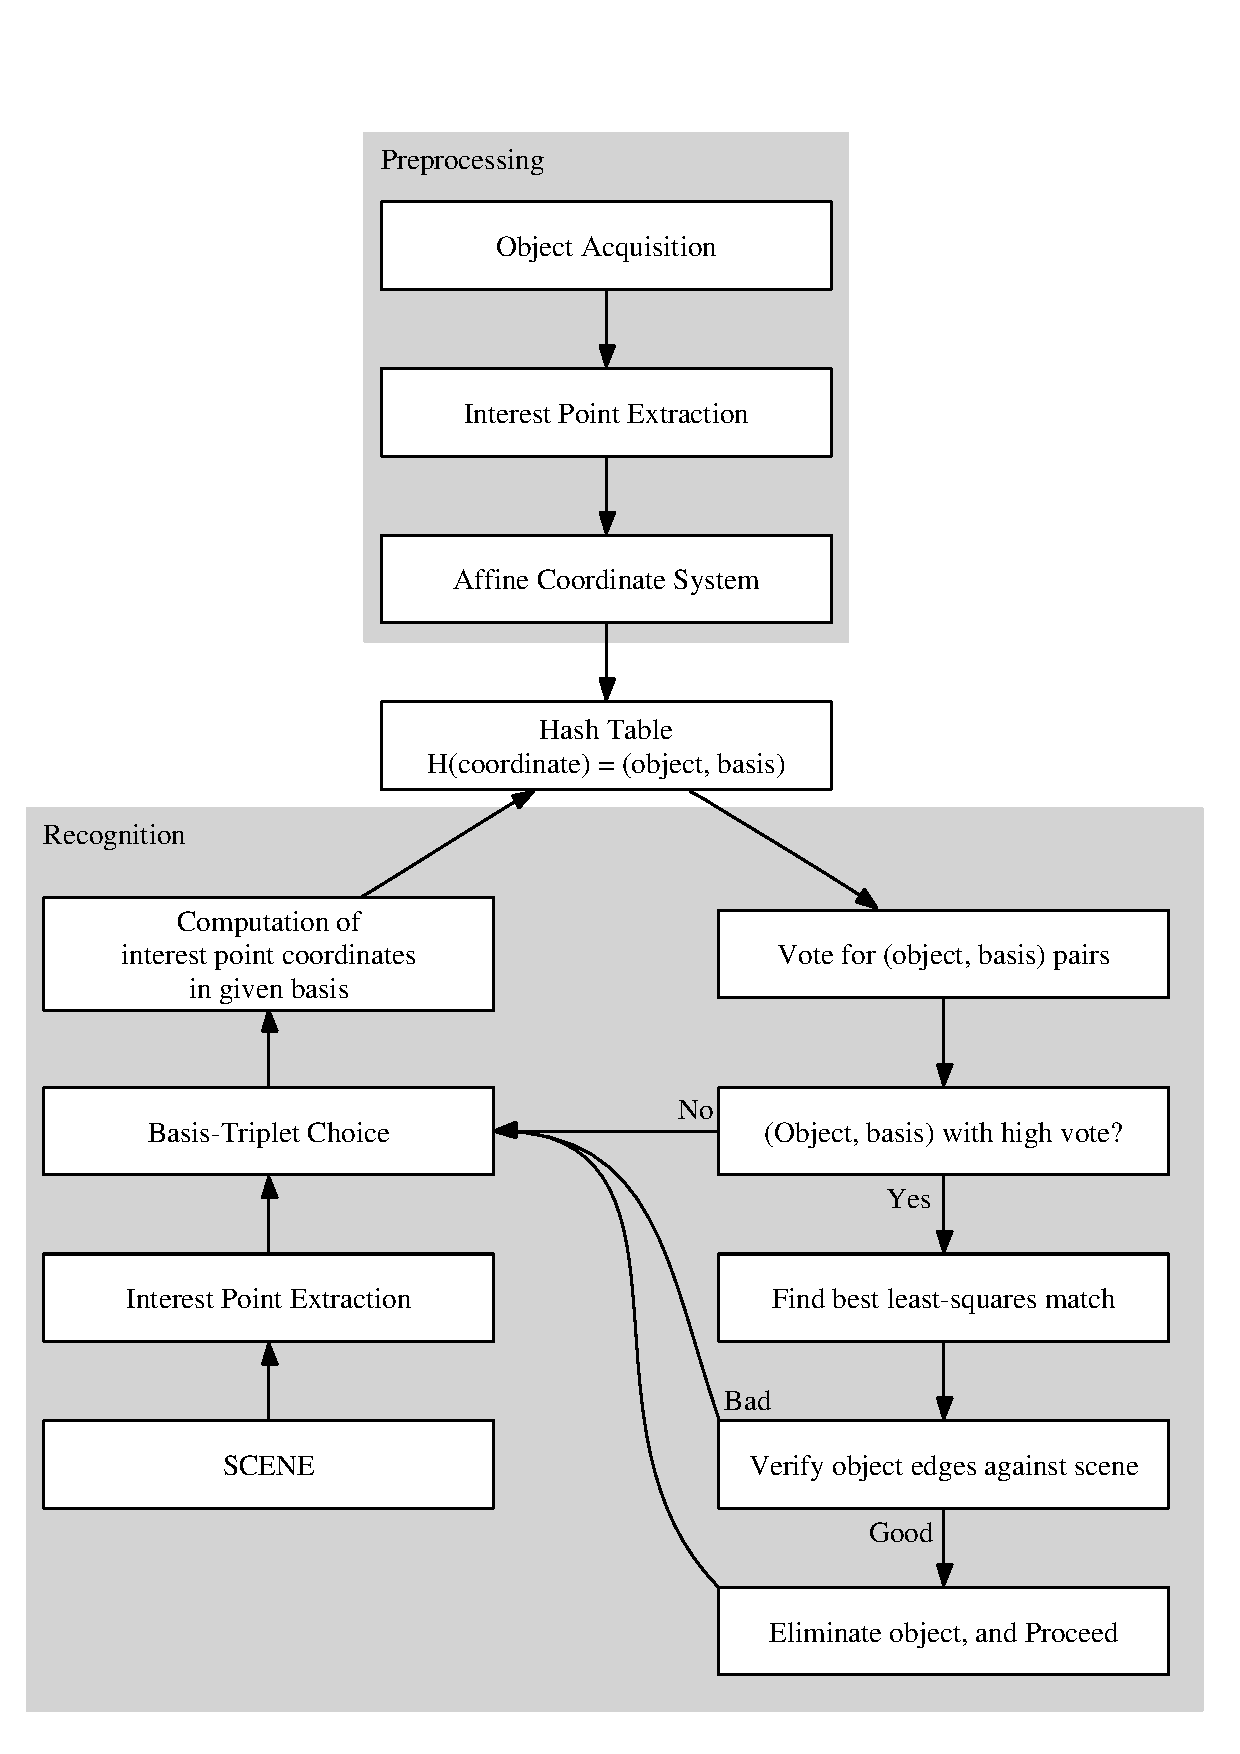
\includegraphics[height=0.8\textheight]{lamdan}
\end{center}
\caption{Outline of the Geometric Hashing scheme.  This diagram is a
  reproduction of \fig 2 in Lamdan \etal \cite{lamdan1990}.
  \label{lamdan}}
\end{figure}


Lamdan \etal \cite{lamdan1990} and Wolfson and Rigoutsos
\cite{wolfson1997} give an excellent overview of the geometric hashing
approach.  See Figure \ref{lamdan} for a block-diagram overview.
Geometric hashing is based on the fact that when rigid objects undergo
similarity transformations (translation, rotation, and scaling),
angles between points on the object and relative distances between
points do not change.  Therefore, if we describe the relative
arrangement of points on an object in terms of these invariants, our
description will be invariant under these transformations of the
object.  Invariant geometric properties can be found for other types
of transformations such as affine or perspective projection.


Geometric hashing builds \emph{geometric features} out of lower-level
features.  We will call the low-level features \emph{interest points}
for clarity.


Given the types of transformations the system must handle, there is
some sufficient number of interest points required to define an
invariant local coordinate system; these are called the \emph{basis
  set}.  For example, for 2-D objects that can undergo similarity
transformations, two interest points can be used to define a
coordinate system.  For 3-D objects with similarity transformations,
three (non-collinear) interest points are required.

Geometric hashing follows an indexing approach.  During the indexing
phase, the system preprocesses a database of objects which are to be
recognized.  For each object, many interest points are extracted which
are invariant under the transformations that are expected, and can be
well localized.  The system then enumerates all basis sets by looking
at all combinations of interest points; each set of basis features
defines a relative coordinate system.  For each basis set, all
remaining interest points are enumerated and their positions described
in this coordinate system.  Each relative coordinate vector forms a
\emph{geometric feature descriptor}.  In this way, the relative
geometric arrangement of a set of interest points is converted into a
point in a vector space.

% --- consider adding a variant of the quad fig here.

In the standard geometric hashing approach, the geometric feature
descriptor is discretized and encoded as a hash table key. A grid is
placed over the feature descriptor space, and the hash table key of a
geometric feature is the identifier of the grid cell containing it.
Each entry in the hash table maps back to the basis set plus the
feature whose position is encoded.

% --- picture?

Given a new image, a geometric hashing system extracts all interest
points from the image and, as at indexing time, proceeds to enumerate
all basis sets and computes the positions of the remaining interest
points in each basis set.  This generates many geometric features
whose descriptors are discretized and converted to hash table keys, as
before.  Similar arrangements of interest points will lead to similar
geometric feature descriptors, which--with luck---will be mapped to
the same hash table key.  The hash table values associated with each
key are retrieved, and each value that is found is considered a match.
Each match votes for the correspondence between the interest points
from the database and the interest points from the image that were
used to define the geometric feature.


After all features from the image have been processed, many votes will
have accumulated.  False matches (due to aliasing or hash table
collisions) should be uniformly distributed over the set of known
objects, so should not generate very many votes for any particular
object.  Objects that are actually present in the image should
generate many votes.  Objects that receive an insufficient number of
votes are rejected, and the remainder are subjected to a verification
process.


The verification process requires computing a transformation from the
object to image coordinates, using the corresponding interest points
from the known object and the image.  Using this transformation, all
the interest points belonging to the known object are projected into
image coordinates.  If the match is correct, we expect the image to
contain features at these locations.  Some researchers add an extra
verification stage by projecting the known object into the image and
checking that the predicted edges of the object are found in the image
(eg, \cite{lamdan1990, huttenlocher1990}).


The geometric hashing approach is flexible and applicable to many
problems, but there are some issues with the basic version described
here.  The hash function described above simply places a grid over the
relative coordinate system and returns the identifier of the grid cell
in which the interest point lands.  This is prone to edge effects: if
an interest point is near the edge of a grid cell, a small change in
its position due to noise can move it across the edge into a different
grid cell, which causes the hash code to change and a different set of
feature matches to be found.  This problem can be overcome by
detecting interest points that are near the edges of their cells and
also searching the hash table using the hash codes of neighbouring
cells.  This results in more false feature matches, and can become
expensive as the dimensionality of the geometric feature space
increases (there are more edges, and the proportion of the hypervolume
of feature space that is near an edge increases).  Using a data
structure other than the hash table may be beneficial.


Another issue with uniform grid-based hashing is that it assigns equal
importance (and storage space) to each grid cell in the feature space.
Consider an interest point that is far from the basis set that defines
its local coordinate system.  Small positional errors in the basis set
can cause the coordinate system to be rotated or scaled, which results
in large changes in the interest point's relative coordinates.  This
means that edge effects become more pronounced in such regions of the
feature space.  One response to this concern is to increases the size
of the grid cells far from the basis set, but then if the interest
points are uniformly distributed, these larger hash table bins will
contain more features, so every match to these bins will be
accompanied by more false positives.


Finally, a hash table with equal-sized cells will only be uniformly
utilized if interest points are uniformly distributed in feature
space, but some domains may yield interest points that are far from
uniformly distributed.  In other domains, it may be beneficial to
place constraints on the geometric features that are used (for
example, to avoid regions that are prone to large errors, or that are
relatively indistinctive).


There is nothing in the geometric hashing framework that requires a
standard hash table to be used for feature matching.  Other methods of
feature matching are described in the next section.


\section{Related work in fast feature matching}


For feature matching in a geometric hashing framework, the database of
known objects is converted into a set of points in a feature
descriptor space, which is a vector space.  To find matches to a new
feature (extracted from an image in which we want to recognize
objects), we need to find all points in the vector space that are
within some tolerance.  Usually the Euclidean distance metric is
applied, so the tolerance is a radius in the vector space.


\subsection{Bloom filters}

A Bloom filter \cite{bloom1970} is a data structure that can answer
queries of the form ``is feature $q$ a member of the set of known
features?''  A Bloom filter is a set of $n$ bits, initially zero.  A
set of $k$ hash functions must be defined which take a feature as
input and produce an integer in $[0, n)$ as output.  In the indexing
phase, we examine each of the known features, and apply each of the
hash functions, producing $k$ hash codes.  Each code is used to
reference a bit and \emph{set} it (\ie, turn it on).  Each known
feature results in $k$ bits being set; several features may request
that a particular bit be set.


Given a new feature to match, we run the $k$ hash functions on it and
test whether each of the resulting bits are set.  If the feature is
equal to a feature seen at indexing time (according to the hash
functions), then all $k$ of the bits will have been set; thus the
Bloom filter does not produce false negatives.  If the query feature
is not equal to a known feature, then some of the bits may have been
set due to \emph{collision} of the hash functions, but the feature
will only be accepted if all $k$ hash functions result in collision;
this results in a false positive.  The rate of false positives
increases as the number of known features increases relative to the
number of bits in the filter.  The Bloom filter is ideally suited to
cases where the number of known features is small, and a verification
step can be applied to eliminate any false positives that are
produced.


For feature matching, we want to know not only whether the query
feature $q$ matches a known feature, we want to know \emph{which}
known feature matches.  One way to answer such queries is to use a
\emph{Bloomier filter} \cite{chazelle2004}.  The simplest Bloomier
filter uses multiple Bloom filters to categorize a given feature into
two different categories, and uses slightly more space than two Bloom
filters.  A set of $n$ such Bloomier filters can be used to categorize
a feature into $2^n$ different categories by assigning one Bloomier
filter to each bit of the result.


The standard Bloom filter only finds exact matches, but we want to
find \emph{nearby} matches.  An extension of Bloom filters to allow
proximity searches is given by Kirsch and Mitzenmacher
\cite{kirsch2006b}.  This variant uses \emph{locality sensitive
hashing} (LSH, discussed below) as its hashing function, so it
inherits some limitations from LSH.  Most importantly, LSH only
guarantees with some probability that nearby features will hash to the
same bin.  As a result, the locality-sensitive Bloom filter can
produce false negatives as well as false positives.


In order to answer feature matching queries (find all known features
near a given query feature), one could combine these Bloom filter
extensions to build a locality-sensitive Bloomier filter.  However,
the false negative rate of the locality-sensitive filter would be
magnified because the Bloomier filter requires \mbox{$2
\ceil{\log(n)}$} separate filters to represent $n$ known features, and
all of these filters must produce the correct answer.  It seems that
Bloom filters are not particularly well suited to this task.


\subsection{Locality Sensitive Hashing}

Locality Sensitive Hashing (LSH) \cite{datar2004, gionis1999,
andoni2006}, is a technique for answering approximate nearest
neighbour queries: it returns a feature whose distance is within a
constant factor of the distance to the nearest neighbour.  The LSH
scheme can be extended to handle exact nearest-neighbour queries
efficiently if the set of known features satisfies some \emph{bounded
growth} criteria.  It is intended for use in high-dimensional spaces
(tens to thousands of dimensions), and $\ell_p$ distance metrics for
$p \in (0, 2]$.


The core idea of LSH is to use several hash functions with the
property that the probability of collision---features being placed in
the same bin---is much higher for nearby features than for distant
ones.  In the indexing stage, we populate the hash table by running
each hash function on each known feature.  To perform a query, we run
the hash functions on the query feature and retrieve the features in
the same hash table bin as the query.  One of these features is likely
to be an approximate nearest neighbour of the query.


In practice, in \cite{datar2004} each hash function is composed of
several (typically $10$) simpler hash functions.  Each simple hash
function performs a random projection in the feature space: the hash
value is the discretized value of the dot product of the feature
vector with the hash function's random vector.  Combining several of
these simple hash functions is equivalent to projecting the feature
vectors onto a grid in a $10$-dimensional, non-orthogonal, subspace.
The hash code is simply the identifier of the grid cell in which the
feature falls.


This scheme suffers from edge effects: a query feature may land in a
bin other than the bin containing its nearest neighbour due to small
positional noise in any of the dimensions.  Attempting to reduce this
effect by making the bin size (discretization level) larger fails
because the number of hash functions must be increased to maintain the
same total number of hash bins.


In order to reduce the number of false negatives, we can choose many
(typically $30$) different hash functions and place a reference to
each feature in the hash table bin chosen by each function.  This
increases the probability that at least one of the hash functions will
select a $10$-dimensional subspace in which the query is close to its
nearest neighbour.


The standard LSH scheme does not seem particularly well suited for the
purpose of feature matching in a geometric hashing system, since the
dimensionality of the feature vectors is usually moderate ($2$ to $6$
in the \an system). Since some feature aliasing is expected in
geometric hashing systems, the nearest neighbour may not be the
correct match: we would prefer to get all neighbours within a given
search radius.


\subsection{\Kdtrees}

\begin{figure}
  \begin{center}
	% tree-figs.py : plot_bboxes
    \begin{tabular}{c@{\hspace{3pt}}c@{\hspace{3pt}}c}
      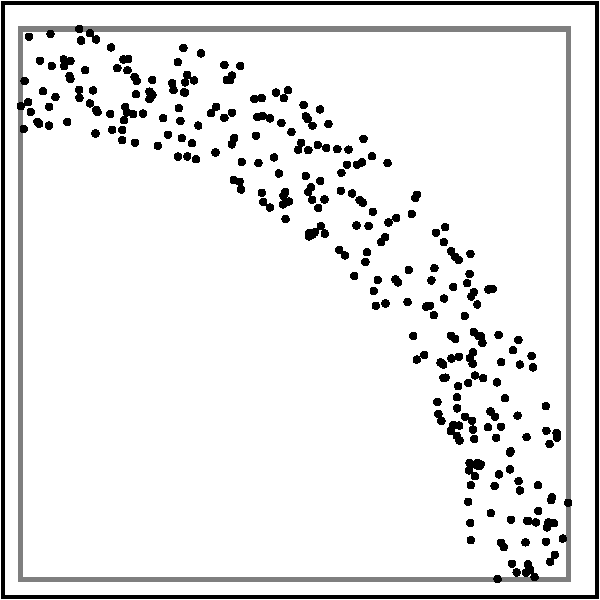
\includegraphics[width=0.31\textwidth]{kdtree-0} &
      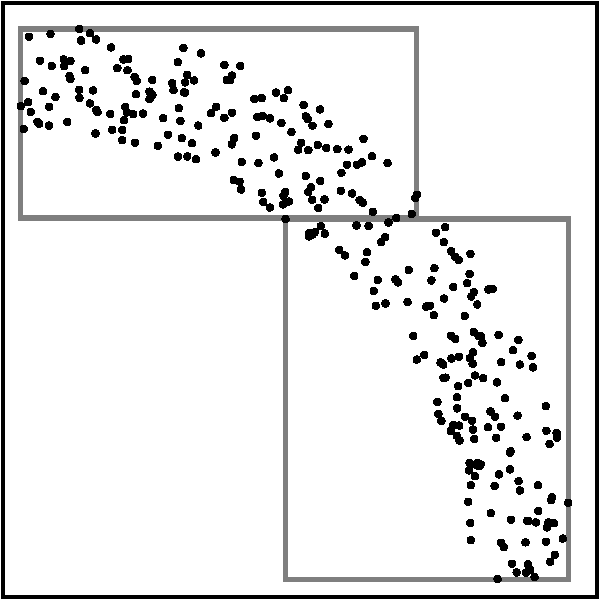
\includegraphics[width=0.31\textwidth]{kdtree-1} &
      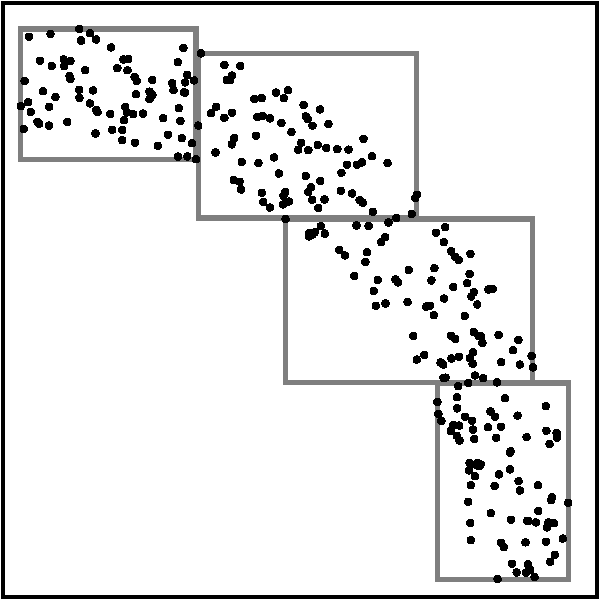
\includegraphics[width=0.31\textwidth]{kdtree-2} \\
      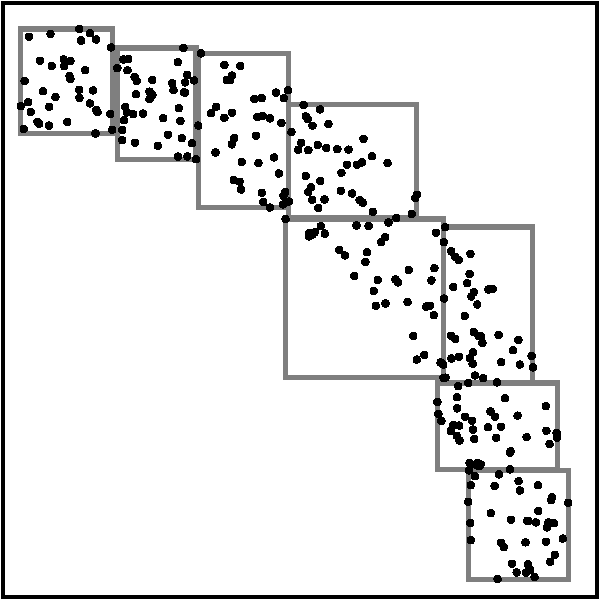
\includegraphics[width=0.31\textwidth]{kdtree-3} &
      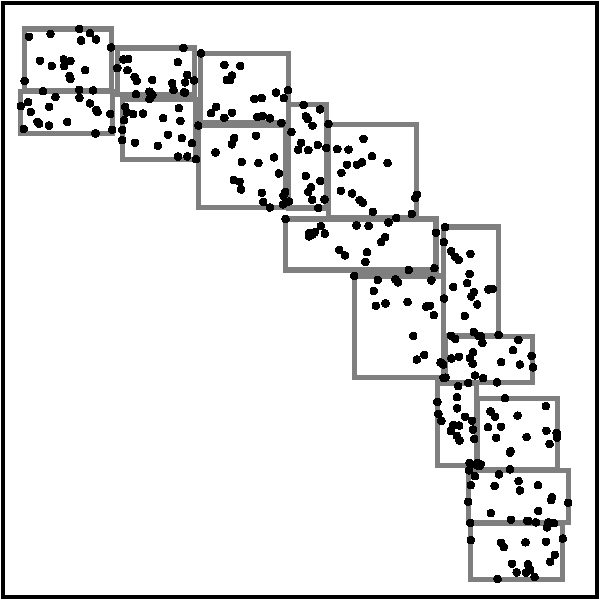
\includegraphics[width=0.31\textwidth]{kdtree-4} &
      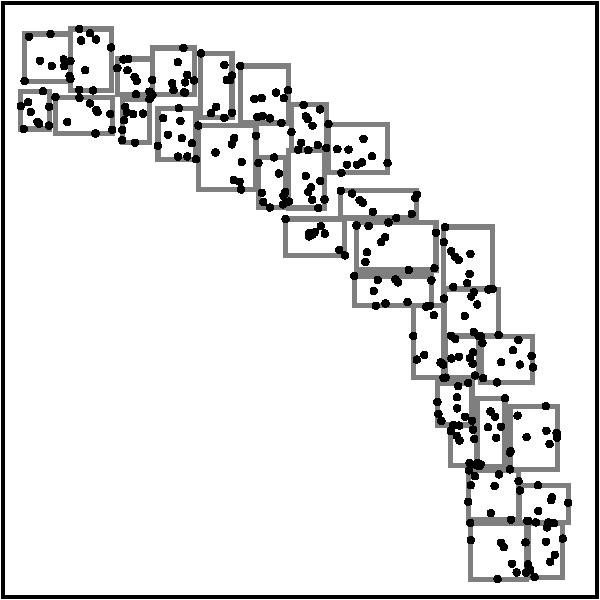
\includegraphics[width=0.31\textwidth]{kdtree-5}
    \end{tabular}
  \end{center}
  \caption[A \kdtree partitioning of space.]{A \kdtree partitioning of
	space.  Each panel shows the nodes at one level of the tree.  The
	points are 200 samples from a ring with uniformly-distributed
	radius in $\left(0.8, 1\right)$ and uniformly-distributed angle in
	$\left(0, \displaystyle{\frac{\pi}{2}}\right)$.  Nodes are split
	along the dimension with the largest range, and the splitting
	position is chosen so that the two child nodes will contain an
	equal number of points.  Note how the tree adapts to the
	distribution of the data: each node tightly bounds the data points
	it owns.  This is a slightly different version of the \kdtree than
	Bentley's original description.\label{kdtree}}
\end{figure}

The $k$-dimensional tree (\kdtree) was introduced by Bentley in 1975
\cite{bentley1975}, and several extensions have been described
\cite{friedman1977, sproull1991}.  The idea is to build a binary tree
over the feature space, where each node ``owns'' a region of the space
which is disjoint from the region owned by its sibling node.  Each
non-leaf node has an axis-aligned splitting hyper-plane; its left
child owns the subspace to the left of the splitting plane, and the
right child the subspace to the right.  In this way, the \kdtree
defines a hierarchical subdivision of the feature space into
axis-aligned hyper-rectangles.  See \figref{kdtree}.


For the purposes of indexing the features in a geometric hashing
system, the set of features is known beforehand and is static, so we
do not need to insert or delete features from the tree, and Bentley's
\emph{optimized} \kdtree construction method can be used.  That is,
the tree can be built to adapt to the particular set of features we
have.


Tree construction proceeds by first assigning all features to the root
node, then recursively splitting nodes until each leaf node owns at
most $L$ features, with $L$ perhaps $10$ or $20$.  Splitting is done
by selecting a splitting plane and using it to partition the features.
Sproull \cite{sproull1991} enumerates several strategies for choosing
the splitting hyperplane.  Traditionally, \kdtrees use axis-aligned
splitting hyperplanes, and the splitting dimension is chosen by simply
iterating through the dimensions (as in Bentley's original paper), or
by selecting the dimension with the largest \emph{range} or
\emph{variance}.  One can also use an arbitrary splitting hyperplane,
for example by finding the principal eigenvector of the covariance
matrix of the feature vectors.  Typically the splitting hyperplane is
positioned so that the two children own an equal number of data
points.  This leads to a balanced (and therefore short) tree, but in
some applications it can be beneficial to bias the splitting location
\cite{macdonald1990}.


Depending on the application, it can be beneficial to store at each
node the tight axis-aligned bounding box (and other summary statistics
\cite{deng1995}) of the points owned by that node (as shown in
\figref{kdtree}).  This is particularly useful where there is
significant correlation between the dimensions of the data, because
splitting the data points along one dimension implies that the
bounding box will shrink in other dimensions as well, and this can
result in faster searches.  If the bounding boxes are stored, then it
is no longer strictly necessary to store the splitting hyperplane,
though it may be useful to speed up some computations.


For feature matching, we typically want to do \emph{range search}:
find all features within radius $r$ of a given query feature $q$.
This is easily achieved with a \kdtree using a recursive algorithm.
Starting at the root, we must decide whether we need to recurse on
each of the node's children.  (How we make this decision is explained
below.)  Once we reach a leaf, we enumerate the features owned by the
leaf and compute the distance to the query feature; any feature with
distance less than $r$ is accepted.


We decide whether we must recurse on a node's children based on their
bounding boxes.  We compute the \emph{mindist}---the lower-bound of
distance---between the query point and each child's bounding box.  The
mindist is simply the distance to the corner or edge of the bounding
box, and can be computed quickly.  Any node whose mindist to the query
point is less than the query radius $r$ must be visited.  If the
\kdtree does not explicitly store the tight bounding-boxes of the
nodes, loose bounding-boxes can be constructed during the recursion
based on the splitting planes of the ancestors.


Chapter \ref{chap:kdtree} presents the \kdtree in more detail.


\subsection{Other approaches}

% Voronoi:
% -de Berg 1997
%   (Mark de Berg , Marc van Kreveld , Mark Overmars , Otfried Schwarzkopf, Computational geometry: algorithms and applications, Springer-Verlag New York, Inc., Secaucus, NJ, 1997)
% -Edelsbrunner 1987
%   (Herbert Edelsbrunner, Algorithms in combinatorial geometry, Springer-Verlag New York, Inc., New York, NY, 1987)
% -Preparata and Shamon 1985
%   (Franco P. Preparata , Michael I. Shamos, Computational geometry: an introduction, Springer-Verlag New York, Inc., New York, NY, 1985)

In contrast to the \kdtree's rectangular decomposition of space, there
is a family of space decompositions that use hyperspheres.  An example
is the \emph{ball-tree} \cite{uhlmann1991b}, in which each non-leaf
node is associated with one of the known features $f$ and a radius
$r$; the left child owns all features within radius $r$ of feature
$f$, and the right child owns the remaining features.  Similarly, in
the \emph{anchors hierarchy} \cite{moore2000}, each non-leaf node is
represented by a feature (called its \emph{anchor}), and a node owns
all the features that are closer to its anchor than the anchor of its
sibling.  These sphere-based trees are supposed to better capture the
structure of high-dimensional data sets, though the results seem to
depend quite strongly on the particular data distributions and search
parameters.


For two-dimensional feature spaces, algorithms based on planar point
location (eg, \cite{kirkpatrick1983}) and the Voronoi tesselation of
space yield $\mathcal{O}(n \log n)$ preprocessing time, a data
structure of size $\mathcal{O}(n)$, and query time of
$\mathcal{O}(\log{n})$.  Unfortunately, in higher dimensions the space
required to store the Voronoi tesselation is
$\mathcal{O}(n^{\floor{d/2}})$, which quickly becomes untenable
\cite{arya1998}.

% planar point location:
% -Dobkin and Lipton in 1976 O((log n)^2) time, O(n^2) space
% -Sarnak and Tarjan O(n) space, O(log n) time
%    * Neil Sarnak, Robert E. Tarjan (1986). "Planar Point Location Using Persistent Search Trees". Communications of the ACM 29 (7): 669-679. 
% -Edelsbrunner, Guibas, and Stolfi, same
%    * Herbert Edelsbrunner, Leonidas J. Guibas, Jorge Stolfi (1986). "Optimal point location in a monotone subdivision". SIAM Journal on Computing 15 (2): 317-340. 
% -Kirkpatrick, same
%    * David G. Kirkpatrick (1983). "Optimal Search in Planar Subdivisions". SIAM J. Comput. 12: 28-35. 
% Voronoi tesselation:
% -B. Delaunay, Sur la sph�re vide, Izvestia Akademii Nauk SSSR, Otdelenie Matematicheskikh i Estestvennykh Nauk, 7:793-800, 1934

The design of spatial indexing data structures and search algorithms
is itself a large research area.  Dozens of different tree structures
have been proposed: in two surveys B\"ohm \cite{bohm2001} and
Hjaltason \cite{hjaltason2003} identify B-, $\textrm{B}^{+}$-, ball-,
bisector-, BSP-, DABS-, fq-, gh-, \mbox{GNA-,} hB-, $\textrm{hB}^{\pi}$-,
hybrid-, IQ-, kd-, kd-B-, $\textrm{LSD}^h$-, M-, mb-,
$\textrm{mb}^{\ast}$-, mvp-, oct-, \mbox{post-office-,} pyramid-, quad-, R-,
$\textrm{R}^{\ast}$-, $\textrm{R}^{+}$-, sa-, slim-, \mbox{sphere-,}
SR-, SS-, TV-, vp-, $\textrm{vp}^{\ast}$-, and X-trees.  There is an
equally mind-boggling variety of exact and approximate search
algorithms.  Each data structure and algorithm may work well in some
region of parameter space, but there is no clear winner for
general-purpose use.


\section{Astrometric calibration as a pattern recognition task}


\comment{
wget "http://casjobs.sdss.org/ImgCutoutDR7/getjpeg.aspx?ra=166.45&dec=-0.03&scale=1&opt=&width=2000&height=2000" -O ngc3521-orig.jpg
jpegtopnm ngc3521-orig.jpg | pnmrotate -45 | pnmcut 600 900 1400 1000 | pnmscale -reduce 2 | pnmtojpeg > ngc3521.jpg
#---> http://live.astrometry.net/status.php?job=alpha-200906-68444159
jpegtopnm ngc3521.jpg | ppmtopgm | pnminvert | pnmtojpeg > ngc3521-bw.jpg
#---> http://live.astrometry.net/status.php?job=alpha-200906-36181848

plotstuff -W 700 -H 500 -J -o ngc3521-sources.pdf < ngc3521-sources.plot
plotstuff -W 700 -H 500 -J -o ngc3521-index.pdf   < ngc3521-index.plot
(at rev 13653)

%%% scp gmaps:/data2/test-merc/tycho.mkdt.fits .
wget "http://explore.astrometry.net/tile/get/?layers=tycho,grid,userboundary&arcsinh&wcsfn=alpha/200906/36181848/wcs.fits&gain=-0.5&bb=0,-85,360,85&dashbox=0.1&w=500&h=500&lw=3" -O ngc3521-zoom0.png
wget "http://explore.astrometry.net/tile/get/?layers=tycho,grid,userboundary&arcsinh&wcsfn=alpha/200906/36181848/wcs.fits&gain=-1&bb=175.533,-17.7621663832,211.533,17.6598478619&dashbox=0.01&w=500&h=500&lw=3" -O ngc3521-zoom1.png
wget "http://explore.astrometry.net/tile/get/?layers=tycho,grid,userboundary&arcsinh&wcsfn=alpha/200906/36181848/wcs.fits&gain=0.5&bb=191.733,-1.85338140354,195.333,1.74602498613&w=500&h=500&lw=3" -O ngc3521-zoom2.png
for x in 0 1 2; do
 pngtopnm ngc3521-zoom${x}.png | ppmtopgm | pnminvert | pnmtopng > ngc3521-zoom${x}-bw.png;
done
}

% ~/an-2/usnob-map/execs/tilerender -x 0.000000 -y -85.000000 -X 360.000000 -Y 85.000000 -w 1024 -h 1024 -l 'tycho' -l 'grid' -l 'boundary' -s -g -0.5 -W 'tor/200706/51145570/wcs.fits' -L 5 -B 0.1 -d > tile1.png
% ~/an-2/usnob-map/execs/tilerender -x 151.724000 -y -4.784223 -X 187.724000 -Y 29.772221 -w 1024 -h 1024 -l 'tycho' -l 'grid' -l 'boundary' -s -g -0.25 -W 'tor/200706/51145570/wcs.fits' -L 5 -B 0.01 -d > tile2.png
% ~/an-2/usnob-map/execs/tilerender -x 167.924000 -y 11.335527 -X 171.524000 -Y 14.841399 -w 1024 -h 1024 -l 'tycho' -l 'grid' -l 'boundary' -s -g 0.5 -W 'tor/200706/51145570/wcs.fits' -L 5 > tile3.png
%
% /home/gmaps/an-2/quads/plotxy2 -i /home/gmaps/ontheweb-data/tor/200706/51145570/index.xy.fits -S 1 -W 720 -H 503 -x 1 -y 1 -w 2 -r 6 -s s > ixy.pgm
% /home/gmaps/an-2/quads/plotxy2 -i /home/gmaps/ontheweb-data/tor/200706/51145570/field.xy.fits -S 1 -W 720 -H 503 -r 5 -x 1 -y 1 -w 2 -s c > fxy.pgm
% cp /home/gmaps/ontheweb-data/tor/200706/51145570/image.pnm undim.ppm
% pgmtoppm green ixy.pgm > ixy.ppm
% pnmcomp -alpha=ixy.pgm ixy.ppm undim.ppm > sum.ppm
% pnmcomp -alpha=fxy.pgm fxy.ppm sum.ppm > sum2.ppm
% pnmtopng sum2.ppm > sum.png
% pnmcomp -alpha=fxy.pgm fxy.ppm undim.ppm | pnmtopng > sources.png
% http://oven.cosmo.fas.nyu.edu/test/status.php?job=tor-200706-51145570


\begin{figure}
\begin{center}
\setlength{\fboxsep}{0.5pt}
\framebox{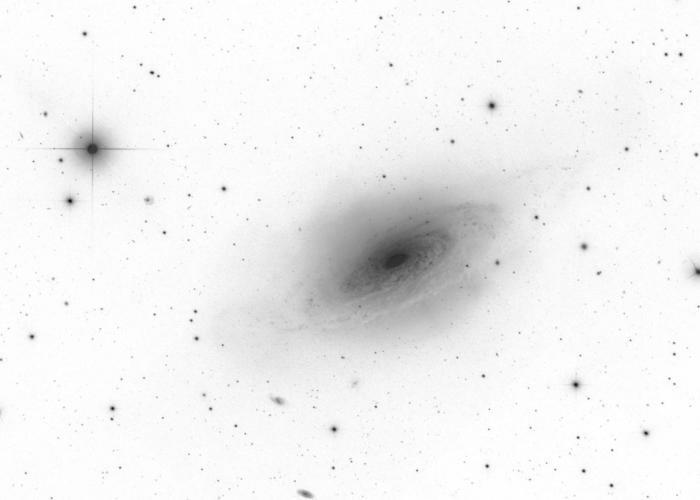
\includegraphics[width=0.99\figunit]{ngc3521-bw}} \\
\framebox{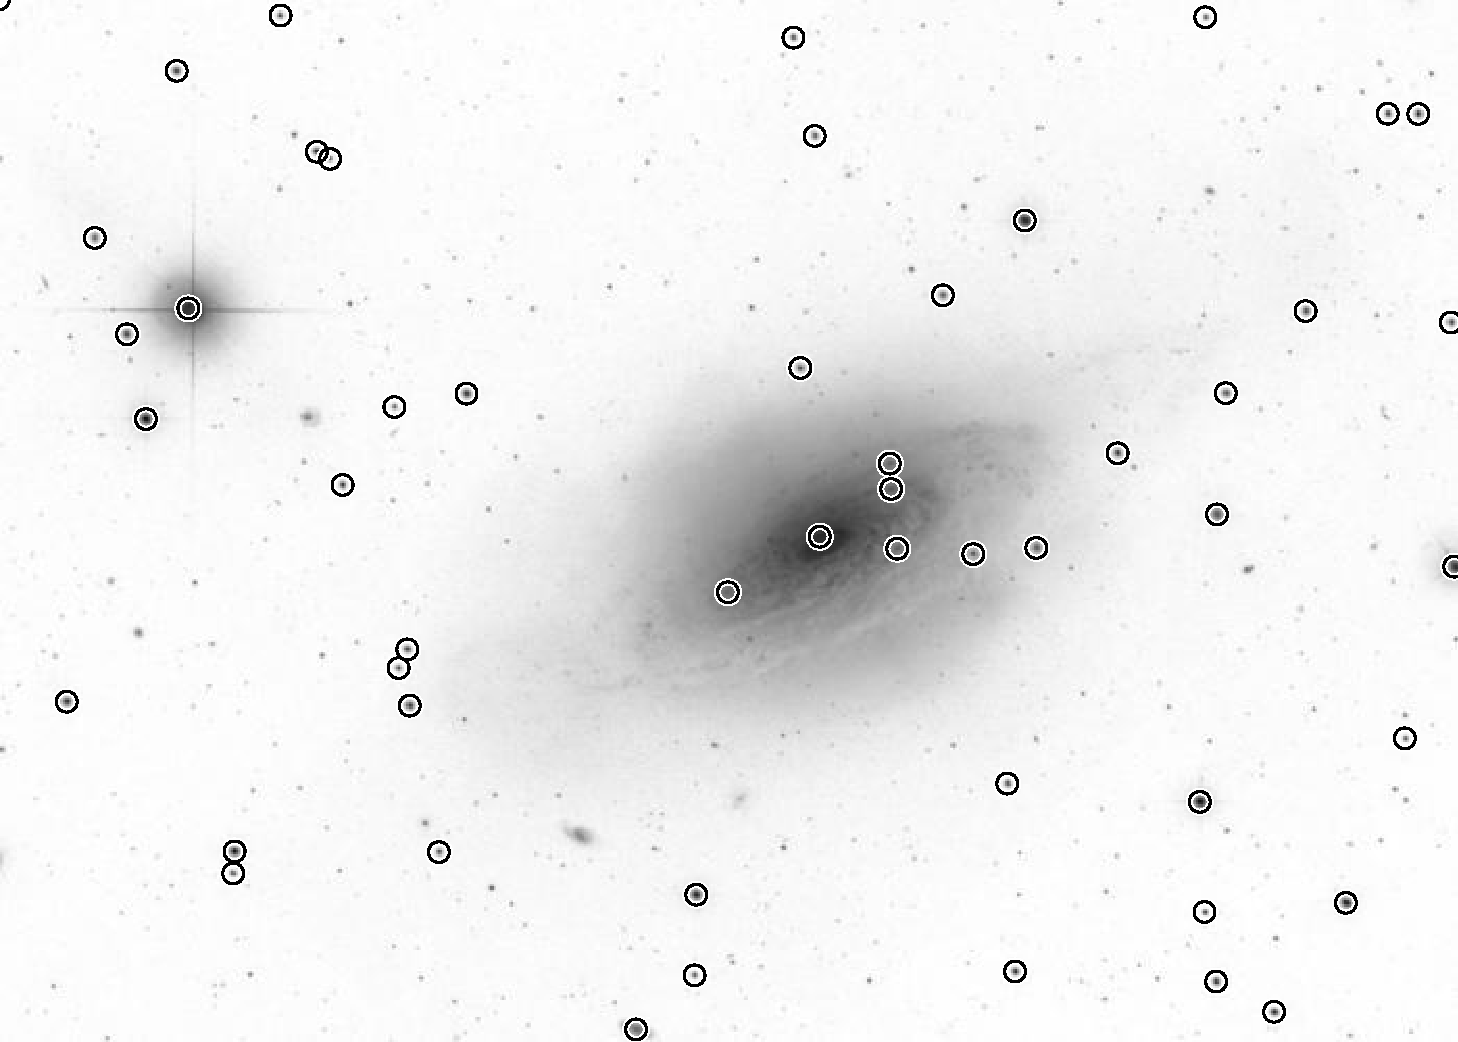
\includegraphics[width=0.99\figunit]{ngc3521-sources}} \\
\framebox{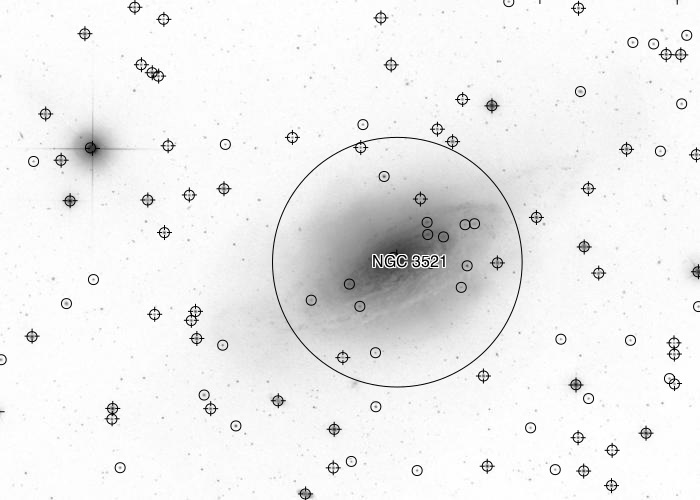
\includegraphics[width=0.99\figunit]{ngc3521-index}}
\end{center}
\caption{\captionpart{Top:} Input image (credit: Sloan Digital Sky
Survey).  \captionpart{Middle:} The brightest 100 sources extracted
from the image.  \captionpart{Bottom:} Reference sources, transformed
into the image coordinate system (crosshairs).  Many of the image and
reference sources are aligned, but there are many image sources
without reference sources.  Our system knows about the positions of
many objects of interest on the sky, and has labelled the galaxy NGC
3521.\label{fig:redgreen}}
\end{figure}


\begin{figure}
\begin{center}
\setlength{\fboxsep}{0.5pt}
\begin{tabular}{c@{\hspace{1pt}}c@{\hspace{1pt}}c}
\framebox{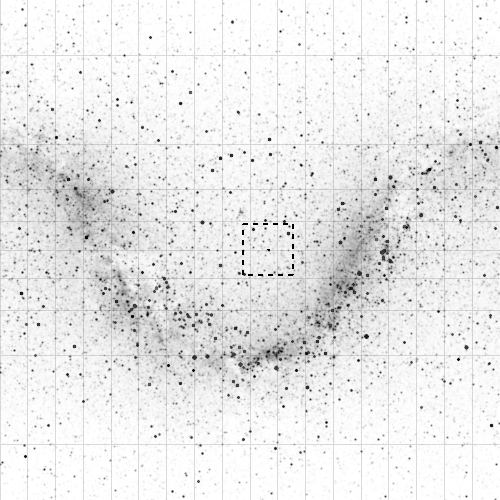
\includegraphics[width=0.31\textwidth]{ngc3521-zoom0-bw}} &
\framebox{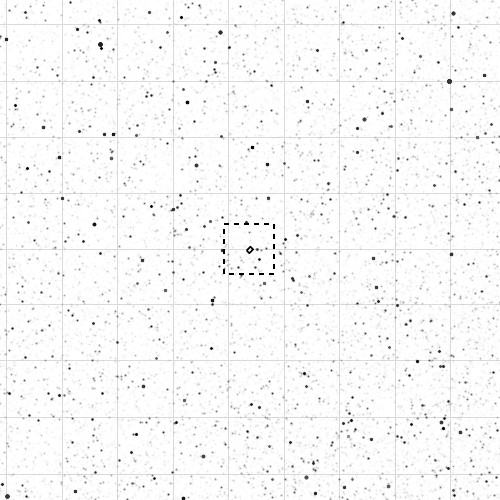
\includegraphics[width=0.31\textwidth]{ngc3521-zoom1-bw}} &
\framebox{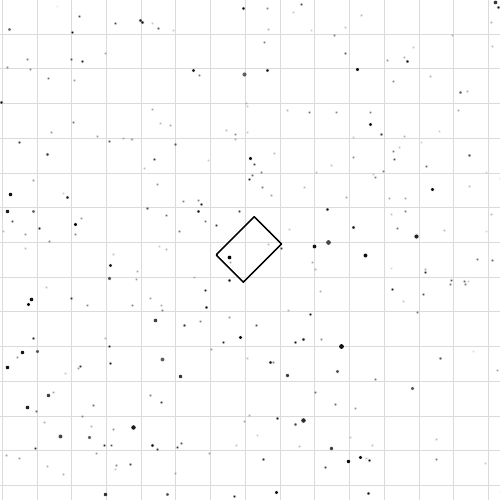
\includegraphics[width=0.31\textwidth]{ngc3521-zoom2-bw}}
\end{tabular}
\end{center}
\caption{The location of the input image on the sky.
  \captionpart{Left:} The whole sky, in Mercator projection.  The
  sinusoid-shaped feature is the Milky Way.  The dashed box shows the
  zoomed-in region.  \captionpart{Middle:} Zoomed in by a factor of
  $10$.  \captionpart{Right:} Zoomed in by a factor of $100$.  The box
  shows the outline of the input image.  These images are rendering of
  stars from the Tycho-2 catalog \cite{tycho2}.\label{fig:onthesky}}
\end{figure}


For modern astronomers, astrometric calibration is often one of the
first steps toward getting useful information out of an image of the
sky.  Aligning a new image with an \emph{astrometric reference
catalog} allows the astronomer to place the image within a standard
coordinate frame.  This allows stars, galaxies, and other objects
(\emph{sources}) in the new image to be identified with known sources,
which in turn allows astronomers to calibrate other properties of the
new image, and allows the positions of new sources to be described in
a standard reference frame.


The task of blind astrometric calibration---automatically finding the
astrometric calibration of an image, using only the information in the
image pixels---can be seen as a pattern recognition problem.  As
Bertin \cite{bertin2005} notes, ``astrometric and photometric
calibrations have remained the most tiresome step in the reduction of
large imaging surveys,'' so this is not only an interesting problem to
solve, but one with practical implications for astronomers.


For the purposes of astrometric calibration, we can think of the sky
as a large two-dimensional surface: the stars are very distant, so our
viewpoint is effectively fixed.  We are moving, as are the stars, but
these motions are small relative to the precision at which we
typically work.  The sky contains many stars, galaxies, and other
astronomical sources.  The stars and distant galaxies are effectively
point sources, while closer galaxies can be resolved.  Astrometric
reference catalogs list the positions, motions, and brightnesses of
these sources and serve as the ``ground truth'' or database of known
(reference) objects.  The USNO-B1 catalog \cite{usnob, nomad}, for
example, lists over one billion objects.  As many as a few percent of
these are false detections or other artifacts \cite{barroncleaning},
and some objects that should be visible are missing.


Extra sources can be due to planets, comets, satellites, or aircraft.
Missing or poorly localized source can be due to imperfections in the
imaging sensor, saturation, cosmic ray interference, or (rarely)
occlusion.  Errors in the image processing that detects sources can
lead to sources being gained or lost.  We call sources that appear in
only the input image or reference catalog \emph{distractors} and
\emph{dropouts}, respectively.  The existence of distractors and
dropouts means that we can never assume that all the objects in the
reference catalog will be contained in an image to be recognized, or
vice versa.


The images to be recognized are subregions of the sky.  Image sizes
range from nearly half the celestial sphere down to $10^{-7}$ of the
area and smaller.  The input images measure unknown bands of the
electromagnetic spectrum, and various nonlinear functions may have
been applied to the pixel values.  We cannot rely on absolute
brightness or color to recognize individual stars or galaxies.  At
best we can hope that there is some positive correlation in the
relative brightness ordering of objects in the image and the
corresponding objects in our catalog.


Blind astrometric calibration is an ideal task for exploring geometric
ideas in pattern recognition.  Most celestial objects are effectively
point sources, and can be found and localized to sub-pixel accuracy
using relatively simple image-processing procedures.  But since the
individual features are characterized only by their positions and
brightnesses, we must examine collections of features in order to
build distinctive patterns.  In \chapref{chap:techreport} we present
\an, which applies the geometric hashing framework to the task of
blind astrometric calibration.  An example of our results in shown in
\figs \ref{fig:redgreen} and \ref{fig:onthesky}.


\section{Related work in astrometric calibration}

There seem to be two distinct groups of researchers who have worked on
astrometric calibration.  The first are professional astronomers,
whose images are typically of small angular extent, long exposure
time, and high quality.  They typically assume that there is a good
initial guess of the astrometric calibration and the goal is to
produce a very accurate calibration, including image distortion.  The
second group of researchers are spacecraft engineers who want to use
the stars to estimate the attitude of a camera attached to a
spacecraft.  Here the images are of wide angular extent, have short
exposure time, and are very noisy.  Primary concerns include weight,
power consumption, and robustness (especially in avoiding false
positives), while a high degree of accuracy is neither required nor
possible given the hardware.

\subsection{Non-blind astrometric calibration}

Non-blind astrometric calibration requires that an initial estimate of
the calibration to be provided.  Groth \cite{groth1986} presents an
algorithm for matching two lists of coordinates (eg, image coordinates
in pixels and reference star coordinates on the celestial sphere),
assuming that the lists contain a significant proportion of objects in
common.  With the limited computing resources available at the time,
he suggests taking the brightest 20 or 30 objects in each list.


Once the two lists of objects have been compiled and the brightest
objects selected, all sets of three objects are enumerated and the
triangles they form are described by a scale-, rotation-, and
translation-invariant descriptor, composed of the length ratio of the
longest to shortest edges, plus the cosine between these edges and the
\emph{sense} or \emph{parity} of the triangle.  The tolerances
associated with these features are computed (by propagating their
positional errors through the feature descriptor process) and stored,
along with the logarithm of the triangle's perimeter.  Triangles with
large length ratio are rejected since they are relatively
indistinctive.


After triangle features are extracted from both point lists, feature
matching is performed by checking whether the distance between each
pair of features is less than their corresponding tolerances.  This
process is accelerated by sorting the features on one of the feature
dimensions.  If multiple matches are found for a particular feature,
only the closest is considered.  After all the features have been
compared, many correct matches should be found, along with some false
matches.  For each match, the difference of the log-perimeters of the
two triangles is computed.  This gives the relative scales of the two
triangles and hence their coordinate frames, assuming the match is
correct.  False matches are rejected by iterative outlier detection:
the mean difference of log-perimeters is computed and matches far from
the mean are rejected.


This approach is essentially an application of the geometric hashing
method, though instead of using hashing to accelerate feature
matching, the features are simply kept in lists that are sorted on one
dimension.  Much of the subsequent work in this area follows
essentially the same path (eg, \cite{valdes1995}, \cite{dong2006}).


P\'al and Bakos \cite{pal2006} adapt the triangle-matching approach to
images containing many more objects (of order $10^4$).  Since it would
become prohibitively expensive to enumerate all triangles in such an
image, they reduce the number of triangles created by using only the
triangles created by a Delauney triangulation.  This vastly reduces
the number of triangles created, but makes the algorithm more
sensitive to dropout and distractor stars: a single extra star causes
a completely disjoint set of triangles to be created in its
neighbourhood.  To compensate for this shortcoming, they define an
\emph{extended Delauney triangulation}: for each point, they select
all points at distance $\ell$ in the Delauney triangulation, and
triangulate this set.  This process is repeated for each point.  The
first extended triangulation ($\ell = 2$) skips over the nearest set
of stars and builds larger triangles by using the next-further set of
stars.  The intent is that if some of the nearby stars are distractors
that they will be ignored when the extended triangulations are used.

\begin{figure}
\begin{center}
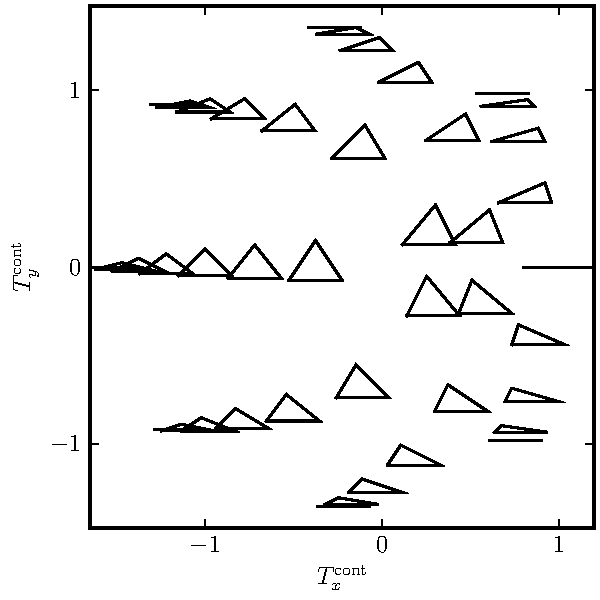
\includegraphics[width=\figunit]{pal-bakos}
\end{center}
\caption{The triangle parameterization used by P\'al and Bakos
  \cite{pal2006}.\label{pal}}
\end{figure}

P\'al and Bakos introduce a new triangle parameterization which is
continuous and sensitive to chirality (parity); see \figref{pal}.
This two-dimensional parameter space is used as the geometric feature
space.  When matching triangles between the two images, they demand a
\emph{symmetric point match}: each triangle must be the other
triangle's nearest neighbour in feature space.  Matching two images is
done by creating the lists of triangles and attempting to find
symmetric point matches.  This process is accelerated by sorting each
list by one of the coordinates.  Each triangle match is considered to
be a vote for the correspondence of the three pairs of points
composing the triangles.  These votes are accumulated in a sparse
matrix where element $(i, j)$ contains the number of votes for a
correspondence between object $i$ in the first image and object $j$ in
the second image.  After all matches are considered, the top 40\% of
the nonzero matrix elements are assumed to contain the true
correspondences.  A transformation based on these correspondences is
computed and the unitarity of the transformation matrix is used to
judge whether the match is true or false.


A different approach is taken by Kaiser \etal \cite{kaiser1999}.  They
assume they are given two lists of source positions that differ by a
rigid transformation involving scaling, rotation, and translation.  In
each image, they iterate over each pair of points and compute the
vector difference of their positions.  For each list, the log-length
and angle of the pairwise difference vectors are accumulated in a
two-dimensional histogram.  Observe that if the whole list of points
is scaled up by a constant factor, then the log-distance between each
pair of points increases by a constant amount.  Similarly, if the
whole list is rotated then the angles shift by a constant amount.
Once the two histograms have been computed, their cross-correlation is
computed.  If the two lists contain a significant number of
corresponding points, the cross-correlation signal will be strongest
at a shift corresponding to the difference in log-scale and rotation
between the lists.  This process is similar to a Hough transform
\cite{duda1972,ballard1981}, except that instead of finding the peak
of a single parameter-space histogram, we are searching for a peak in
the similarity of two histograms as we shift them with respect to each
other in parameter space.


Once the scaling and rotation between the lists has been found, the
translation can be found by scaling and rotating one of the lists into
the frame of the other list, then histogramming the vector difference
between points across the two lists.  This is a standard (generalized)
Hough transform.


\subsection{Blind astrometric calibration}


The majority of previous work on blind astrometric calibration is
motivated by the problem of spacecraft attitude estimation.  Sometimes
called the ``lost in space'' or ``stellar gyroscope'' problem, the
task is to estimate the pose of a spacecraft by using an image of the
sky captured by an onboard camera.  Although similar in general
spirit, the requirements and limitations of this application are quite
different than astronomical applications.  Mass, power consumption,
and robustness of the system are primary concerns, and as a result the
optical designs are very different from science-grade astronomical
instruments, and the available processor and memory resources are very
restricted.  Typical fields of view are tens of degrees across, and
the exposure time is kept short to allow the system to function while
the spacecraft is rotating.  As a result, image quality is typically
quite poor: often only a handful of the brightest stars are visible.
Since the field of view is large, a reference catalog of a few
thousand stars is sufficient to ensure that any view of the sky
contains many reference stars.  Since the system will only process
images from a single camera, the whole system can be customized and
calibrated to that camera.  For example, the nonlinear distortions of
the optical system can be measured, and the scale and bandpass of the
imaging system are known, so the reference catalog can be tailored to
match.


For example, Liebe \etal \cite{liebe2004} describe a system design
with a $56~\deg$ field of view and exposure time of $50~\unit{ms}$.
The resulting images contain tens of stars if the spacecraft is not
rotating, but on average only three stars will be detectable when the
rotation rate is $50~\deg/\unit{sec}$.  The paper does not describe a
particular algorithm for star identification, with the implication
that it is not a particularly difficult problem since absolute
brightness information will be available, and the total number of
stars that are visible to the camera is only a few hundred.


In earlier work \cite{liebe1993}, Liebe describes a star
identification system.  The reference catalog is composed of the $1539$
brightest stars, with brightness calibrated to the camera used in the
system.  The field of view is $30~\degrees$, and the system uses a
feature-matching approach, using the brightest star in the field and
its two nearest neighbours to define a geometric feature.  The feature
descriptor is composed of the distance from the brightest star to its
nearest and second-nearest neighbours, along with the angle between
these neighbours.  Note that this feature is not scale-invariant:
the system is only meant to recognize images taken by one camera,
so the scale is known.  An index is constructed by enumerating all
such features that could possibly be detected, given the detection
limits of the camera.  These features are coarsely quantized and
stored in a table.  To account for noise in the feature descriptors,
all neighbouring cells in the quantized feature space are also stored
in the table.  This generates $185,000$ features.  At test time, the
features in the image are enumerated and the table of features is
scanned; an exact feature match in the quantized space is assumed to
be correct.


This approach is a fairly straightforward geometric hashing technique,
except that it does not use hashing as such, and there is no voting or
verification scheme because feature aliasing is assumed not to happen.

\begin{figure}
\begin{center}
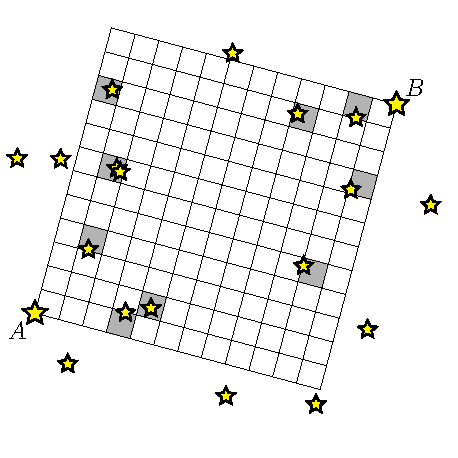
\includegraphics[width=\gridfigwidth]{grid-fig}
\end{center}
\caption{A grid-based feature: two sources (labelled $\starA$ and
  $\starB$ here) are used to define a local coordinate system which is
  discretized into a grid of cells.  Each cell becomes a bit in the
  feature descriptor; if a cell is occupied by a star its bit is set.
  This figure is inspired by MacKay \& Roweis \cite{mackay2005}.}
\label{gridbased}
\end{figure}

In contrast to systems that build features from the precise locations
of a small number of stars, Padgett and Kreutz-Delgado
\cite{padgett1997} present an approach that incorporates information
from a large portion of the image.  Their grid-based feature is
defined by first choosing one star as the reference star to define the
center of the grid, then selecting its nearest neighbour (outside an
exclusion radius) to define the orientation of the grid.  Once the
center and orientation are determined, a grid is defined, and each
remaining stars in the image is assigned to a grid cell.  The feature
is a bit vector, one bit per grid cell, where the bit is set only if
the cell contains a star.  See \figref{gridbased}.


The index is constructed by scanning the sky and selecting, for each
field of view, the $n$ brightest stars.  For each of these stars a
feature is computed and stored.  At test time, they examine the
brightest $c n$ stars (for some safety factor $c$), computing the
feature for each one and searching the index for a match.  A pair of
features is defined to match if their dot product is above a
threshold.  This is equivalent to taking the bitwise \textsc{AND} of
the bit vectors and counting the number of bits that are set.  This
search can be implemented efficiently by using lookup tables: for each
bit, they maintain a list of the features for which that bit is set.
Note that this is equivalent to using a grid-based geometric hashing
approach: each grid cell is equivalent to a discretized relative
coordinate vector, which becomes a hash key, and the ``lookup table''
is a hash table.  After all the features in the test image have been
extracted and matched to the index, the algorithm proceeds to a voting
(or perhaps ``consensus'') phase where it rejects matches that propose
a field of view that does not overlap that of the majority.


The system is designed to operate on images of diameter $8~\degrees$,
and performs well on simulated data.  They use a grid size of $40
\times 40$, and find that on average $25$ grid cells are filled.
Their index contains $13,000$ patterns, which means that false
positives are quite rare.  However, misidentification of the nearest
neighbour, or edge effects (assigning a star to the wrong grid cell
due to positional noise) mean that failures to find a match are not
uncommon, and are more likely in regions of the sky with high stellar
density.

In later work, Clouse and Padgett \cite{clouse2000} extend this
approach by using Bayesian decision theory instead of a simple
threshold on the dot product to define how well features match.  This
extension, along with smaller noise levels in the (simulated) imaging
system, allows them to extend the approach down to fields of view
$2~\degrees$ in diameter.

\comment{
  Given two features, they compute the dot product between the bit
  vectors, then proceed to estimate the probabilities that the match is
  a true positive and false positive.  These probability distributions
  are quite complex, so several simplifying approximations are made, and
  the remaining parameters are estimated by running simulations.
  }

Harvey \cite{harvey2004} presents two different approaches, one
grid-based and the other shape-based.  The grid-based approach is
similar to the Padgett--Kreutz-Delgado and Clouse--Padgett approaches
\cite{padgett1997, clouse2000}.  A coarser grid is used, so more stars
are likely to appear in each bin.  To compensate, a grid cell is only
considered ``occupied'' if it contains more than some threshold number
of stars.  The other major change is that he expects a test image to
be an ``overexposure'' or ``underexposure'' relative to the reference
catalog.  This implies that the test image should contain either a
subset or a superset of the stars in the index, and therefore the
image feature vector must be either greater than or less than an index
feature at each bit.  This allows simple bit operations to be used to
find feature matches, and feature matching is performed by a linear
scan through the index.

Harvey's shape-based approach uses constrained $n$-star constellations
in order to aggregate information from a large number of stars without
allowing the number of potential features to grow combinatorially.
Specifically, Harvey uses a pair of stars to define a narrow wedge in
the image, then describes the relative positions and angles of a fixed
number of nearby stars within that wedge.  Unfortunately, this makes
the feature highly sensitive to distractor and dropout stars, since
the feature depends on the stars in the feature being enumerated in a
particular order.  As a result, all potential features (allowing any
combination of stars to drop out) must be checked; the number of
features grows exponentially as the density of stars increases.


Harvey makes the useful observation that a cascade of indices can be
built, where each index is designed to recognize images with a particular
range of scales.


MacKay and Roweis \cite{mackay2005} point out that a grid-based
feature such as that used by Harvey leads naturally to a hashing-based
strategy.  Each grid cell is associated with a bit that is turned on
if the cell is occupied.  This value is placed in a hash table with a
mapping back to its position on the sky.  Since false positives can
occur as a result of feature aliasing or hash collision, a voting
scheme is employed: several feature matches must accumulate before the
match is accepted.  Since false negatives can occur as a result of
dropouts and distractors (\emph{any} missing or extra star causes the
hash code to change completely), many features must be extracted for
each region of the sky.


\subsection{Fine-tuning astrometric calibrations}

In order to ``co-add'' or ``stack'' astronomical images (combine
pixels from different images to produce a higher signal-to-noise
image), or to do proper-motion studies (measure the movement of stars
over time), it is necessary to fine-tune the astrometric calibration
of the images.  This is similar to the \emph{bundle adjustment}
problem in computer vision \cite{triggs2000}, in that it involves the
simultaneous optimization of the various camera and telescope
parameters and the estimated positions of objects in the world.
Fine-tuning astrometric calibrations is easier because it is
essentially two-dimensional, but more difficult because the camera
parameters include polynomial distortion terms to model the image
distortion introduced by telescope optics.


The software package \scamp by Bertin \cite{bertin2005} is a popular
tool used by astronomers to fine-tune simultaneously the astrometric
calibrations of a large collection of images.  For each image, it is
assumed that the center of the image is known to about 25\% of the
size of the image, and the scale is known to within a factor of two.
The histogram-alignment method of \cite{kaiser1999} is used to find
the translation, scaling, and rotation between the image and a
reference catalog, which allows the correspondences between image and
reference catalog stars to be determined.

The core of the \scamp system is a chi-squared minimization of the
total weighted distance between the projected positions of all star
correspondences among the set of images and the reference catalog.
The parameters to be adjusted are the center, scale, rotation, and
polynomial distortion coefficients of each image.  A key feature is
the ability to share image distortion parameters among subsets of the
images, since images taken with the same telescope are expected to
share some distortion terms due to the telescope optics.  This reduces
the degrees of freedom of the fitting process, resulting in more
robust fits.  \scamp can fine-tune thousands of images to sub-pixel
accuracy.


\section{Summary}


The task of automatically finding the astrometric calibration of an
astronomical image---this is, recognizing the stars in the image, or
locating the image on the sky---is ideal for a geometric hashing-based
approach.  Geometric hashing (or more generally, geometric feature
matching) is a widely-applicable technique for problems in which it is
desirable to build distinctive geometric features out of simple
interest-point features.  The approach is ideally suited to the blind
astrometric calibration problem, since images of celestial objects can
be localized to sub-pixel accuracy but have few other distinguishing
features.  Indeed, much of the previous work in blind and non-blind
astrometric calibration can be placed within a geometric feature
matching framework.




\chapter[\antitle: recognizing astronomical images]
		{\an: recognition of arbitrary astronomical images%
		  \footnote{This chapter was originally prepared as a manuscript
			by me, David~W.~Hogg, Keir~Mierle, Michael~Blanton, and
			Sam~Roweis.}}
\label{chap:techreport}
\graphicspath{{figs-techreport/}}
\input{tech-report-common}
%% Common definitions, defined in sdss-er.tex
\newlength{\pointonesec}\settowidth{\pointonesec}{$0.1$ s}
\newlength{\acceptable}\settowidth{\acceptable}{Acceptable}

\newcommand{\sdssertable}{\begin{tabular}{|c|D{.}{.}{6.0}|D{.}{.}{6.0}|D{.}{.}{3.2}|}
\hline
\multicolumn{1}{|c|}{\textbf{Phase}} & \multicolumn{1}{c|}{\textbf{Images recognized}} & \multicolumn{1}{c|}{\textbf{Unrecognized}} &
\multicolumn{1}{c|}{\textbf{Percent recognized}} \\
\hline
\usnob: \makebox[\pointonesec][r]{$0.1$ s} & 172,882 & 9,339 & 94.87 \\
\usnob: \makebox[\pointonesec][r]{$1$ s} & 181,826 & 395 & 99.78 \\
\usnob: \makebox[\pointonesec][r]{$10$ s} & 182,158 & 63 & 99.97 \\
\usnob: \makebox[\pointonesec][r]{$15$ s} & 182,160 & 61 & 99.97 \\
\twomass & 182,211 & 10 & 99.99 \\
Original images & 182,221 & 0 & 100.00 \\
\hline
\end{tabular}
}

\newcommand{\sdsserradecfig}{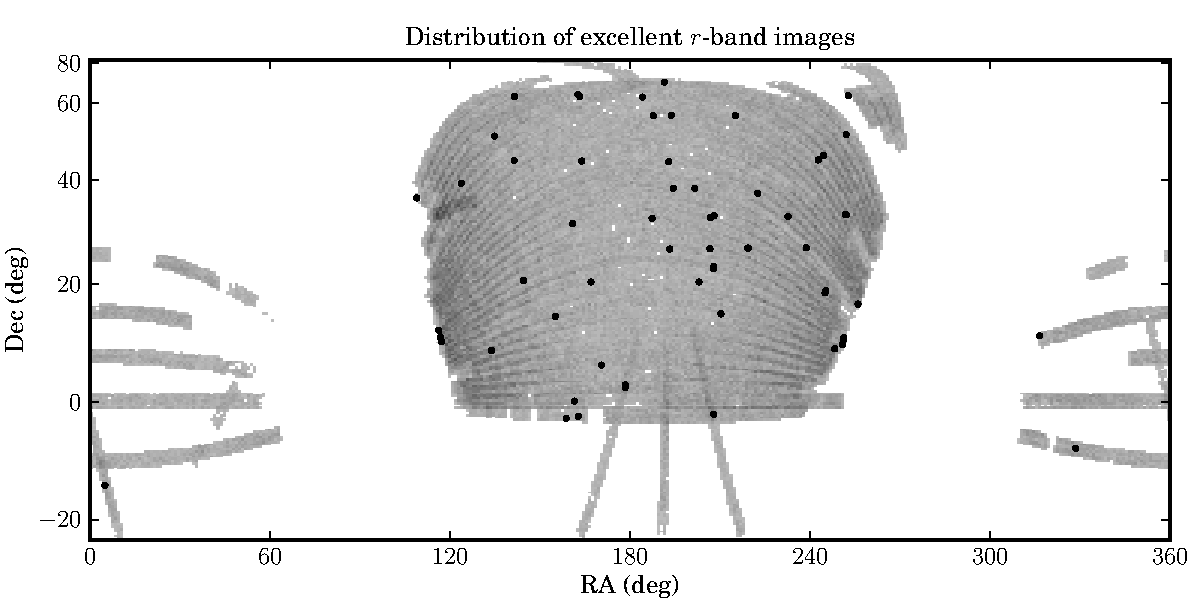
\includegraphics[width=2.000000\figunit]{sdss-er-radec}}
\newcommand{\sdssercputimefig}{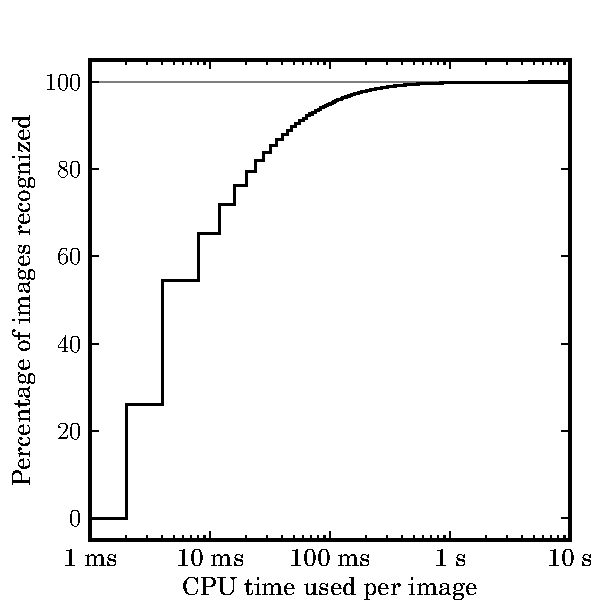
\includegraphics[width=1.000000\figunit]{sdss-er-cputime}}
\newcommand{\sdssernimagefig}{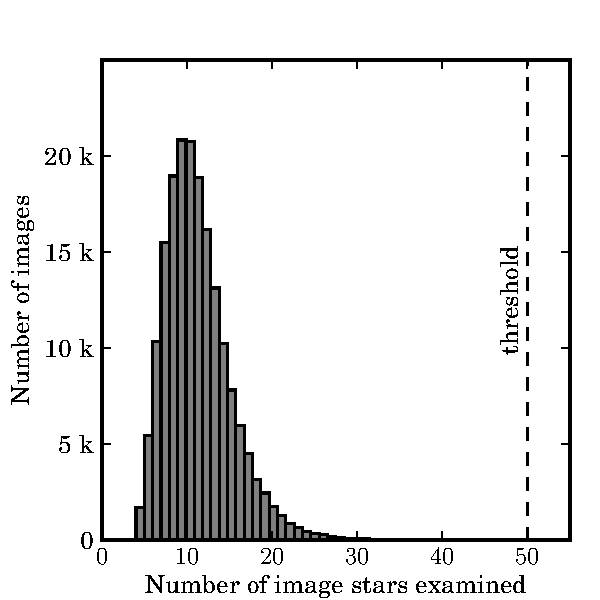
\includegraphics[width=1.000000\figunit]{sdss-er-nimage}}
\newcommand{\sdssernmatchfig}{\includegraphics[width=1.000000\figunit]{sdss-er-nmatch}}
\newcommand{\sdssercodeerrfig}{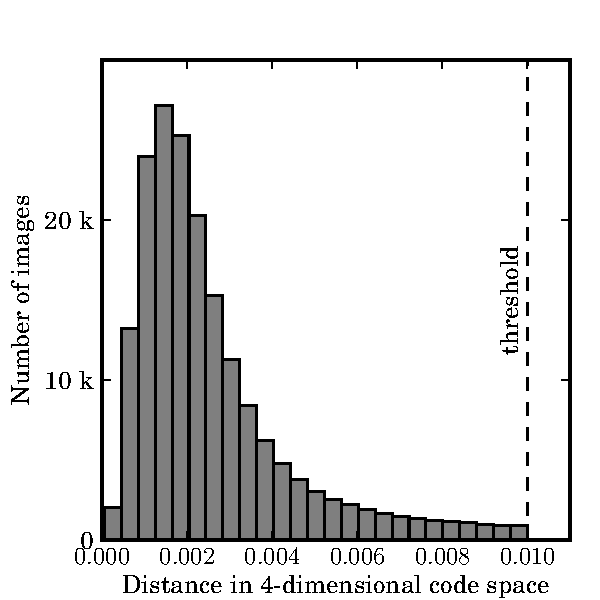
\includegraphics[width=1.000000\figunit]{sdss-er-codeerr}}
\newcommand{\sdsserbayesfig}{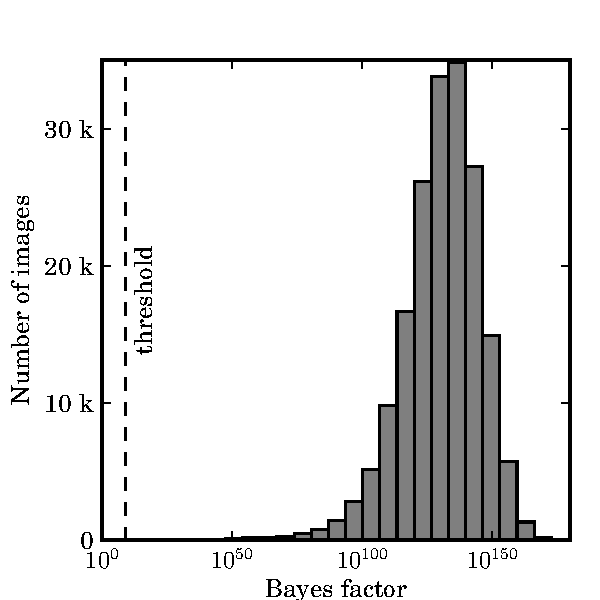
\includegraphics[width=1.000000\figunit]{sdss-er-bayes}}

\newcommand{\sdsserntoverifyfig}{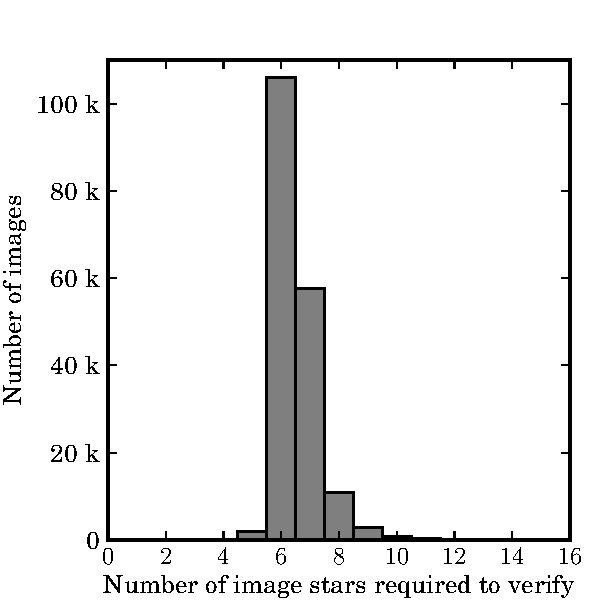
\includegraphics[width=1.000000\figunit]{sdss-er-ntoverify}}
\newcommand{\sdssbandtable}{\begin{tabular}{|c|D{.}{.}{3.2}|D{.}{.}{3.2}|D{.}{.}{3.2}|D{.}{.}{3.2}|D{.}{.}{3.2}|}
\hline
\multicolumn{1}{|c|}{\textbf{CPU time}} &\multicolumn{5}{c|}{\textbf{Percentage of images recognized}} \\
\cline{2-6}
\multicolumn{1}{|c|}{(per image)} & \multicolumn{1}{c|}{$u$} & \multicolumn{1}{c|}{$g$} & \multicolumn{1}{c|}{$r$} & \multicolumn{1}{c|}{$i$} & \multicolumn{1}{c|}{$z$} \\
\hline
\makebox[\pointonesec][r]{$0.1$ s} & 87.80  & 93.88  & 94.87  & 93.59  & 94.36 \\
\makebox[\pointonesec][r]{$1$ s} & 98.58  & 99.73  & 99.78  & 99.73  & 99.75 \\
\makebox[\pointonesec][r]{$10$ s} & 99.82  & 99.96  & 99.97  & 99.96  & 99.96 \\
\makebox[\pointonesec][r]{$60$ s} & 99.84  & 99.96  & 99.97  & 99.96  & 99.96 \\
\hline
\end{tabular}
}
\newcommand{\sdssbandsobjsfig}{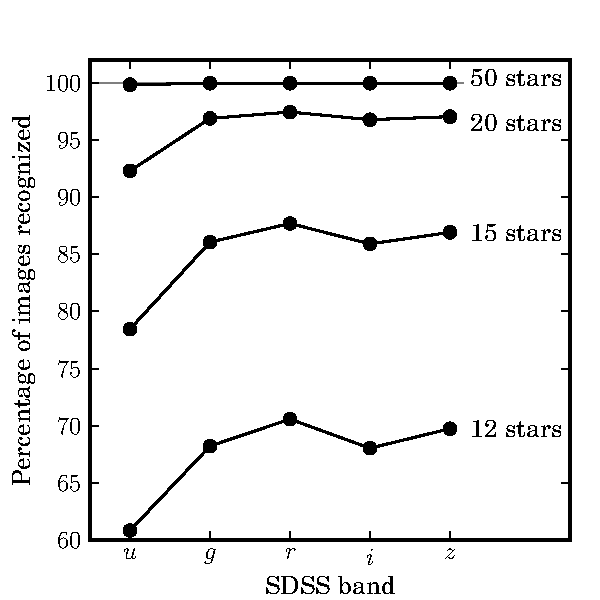
\includegraphics[width=1.000000\figunit]{sdss-bands-objs}}
\newcommand{\sdssbandstimefig}{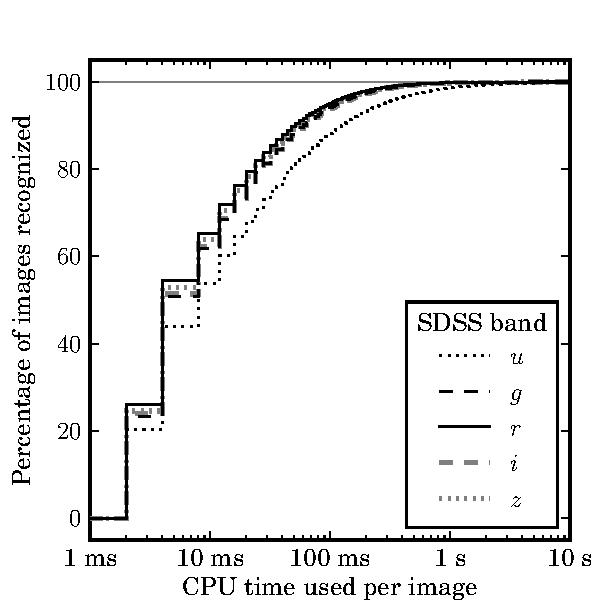
\includegraphics[width=1.000000\figunit]{sdss-bands-time}}
\newcommand{\sdssqualtable}{\begin{tabular}{|c|D{.}{.}{3.2}|D{.}{.}{3.2}|D{.}{.}{3.2}|D{.}{.}{3.2}|}
\hline
\multicolumn{1}{|c|}{\textbf{CPU time}} &\multicolumn{4}{c|}{\textbf{Percentage of images recognized}} \\
\cline{2-5}
\multicolumn{1}{|c|}{(per image)} & \multicolumn{1}{c|}{\makebox[\acceptable][c]{Excellent}} & \multicolumn{1}{c|}{\makebox[\acceptable][c]{Good}} & \multicolumn{1}{c|}{\makebox[\acceptable][c]{Acceptable}} & \multicolumn{1}{c|}{\makebox[\acceptable][c]{Bad}} \\
\hline
\makebox[\pointonesec][r]{$0.1$ s} & 94.87  & 94.85  & 94.57  & 84.11 \\
\makebox[\pointonesec][r]{$1$ s} & 99.78  & 99.74  & 99.64  & 96.58 \\
\makebox[\pointonesec][r]{$10$ s} & 99.97  & 99.94  & 99.94  & 99.11 \\
\makebox[\pointonesec][r]{$60$ s} & 99.97  & 99.94  & 99.95  & 99.18 \\
\hline
\end{tabular}
}
\newcommand{\sdssqualtimefig}{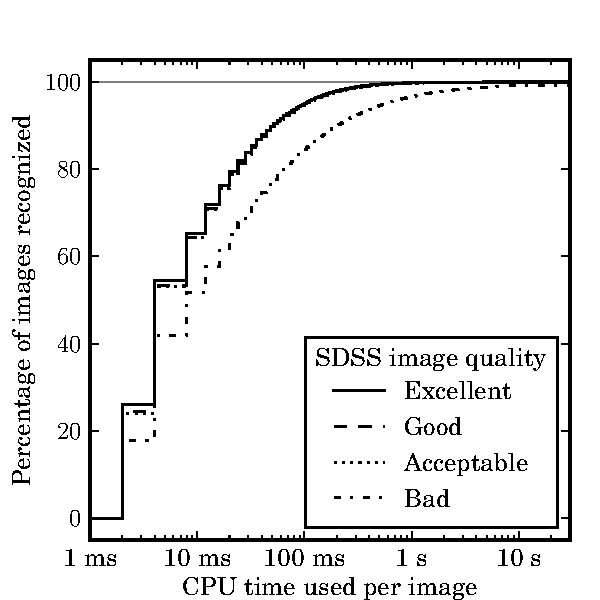
\includegraphics[width=1.000000\figunit]{sdss-qual-time}}
\newcommand{\sdssqualobjsfig}{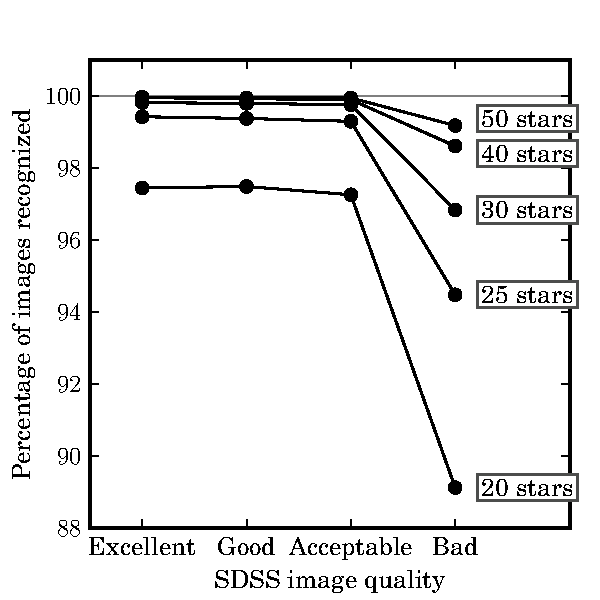
\includegraphics[width=1.000000\figunit]{sdss-qual-objs}}
\newcommand{\sdssimsizetimefig}{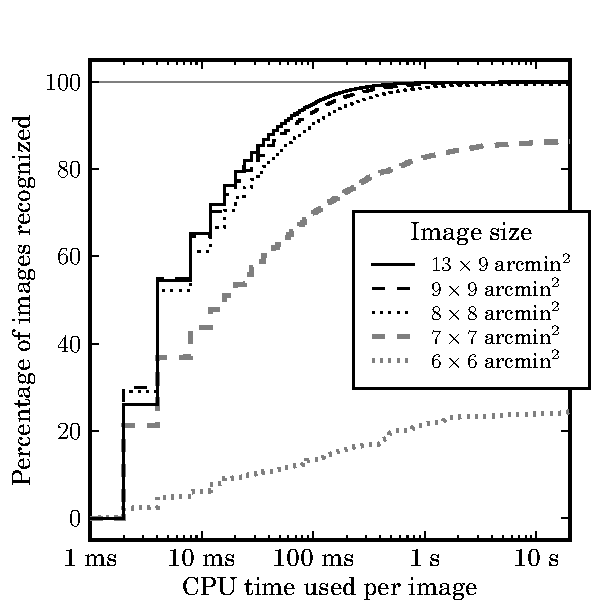
\includegraphics[width=1.000000\figunit]{sdss-imsize-time}}
\newcommand{\sdssimsizetable}{\begin{tabular}{|D{x}{\times}{2.1}|D{.}{.}{3.2}|}
\hline
\multicolumn{1}{|c|}{\textbf{Image size (arcmin${}^2$)}} &
\multicolumn{1}{c|}{\textbf{Percentage of images recognized}} \\
\hline
13x9 & 99.97\\
9x9 & 99.88\\
8x8 & 99.52\\
7x7 & 86.53\\
6x6 & 24.75\\
\hline
\end{tabular}
}
\newcommand{\sdssimsizeobjsfig}{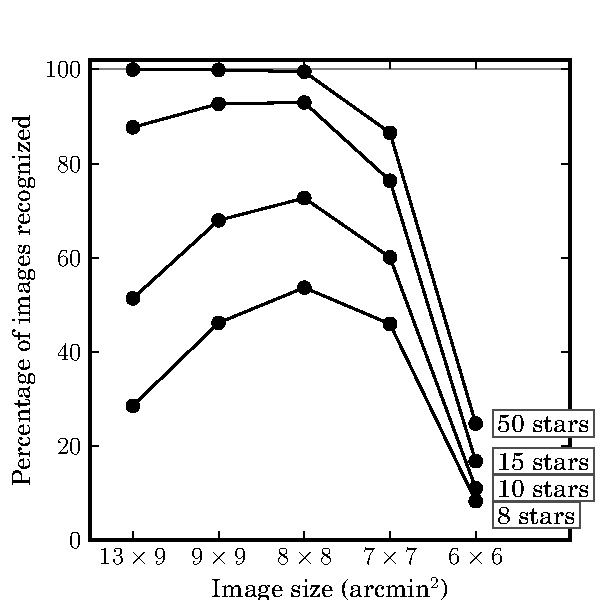
\includegraphics[width=1.000000\figunit]{sdss-imsize-objs}}
\newcommand{\sdsssizehintsreltimefig}{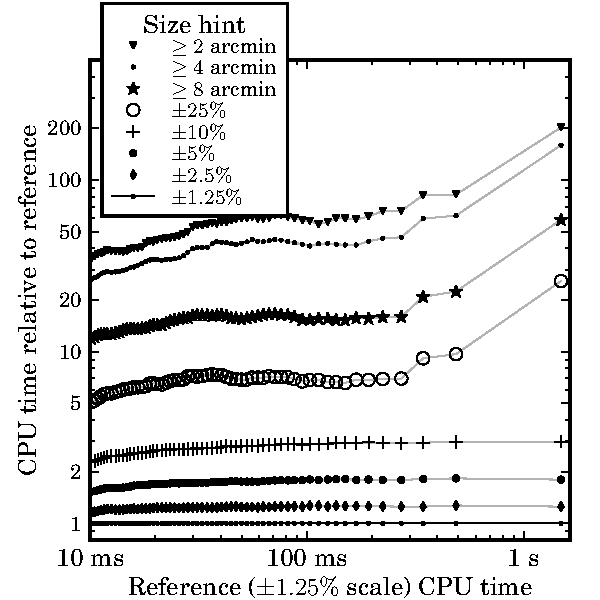
\includegraphics[width=1.000000\figunit]{sdss-sizehints-reltime}}
\newcommand{\sdsssizehintstimefig}{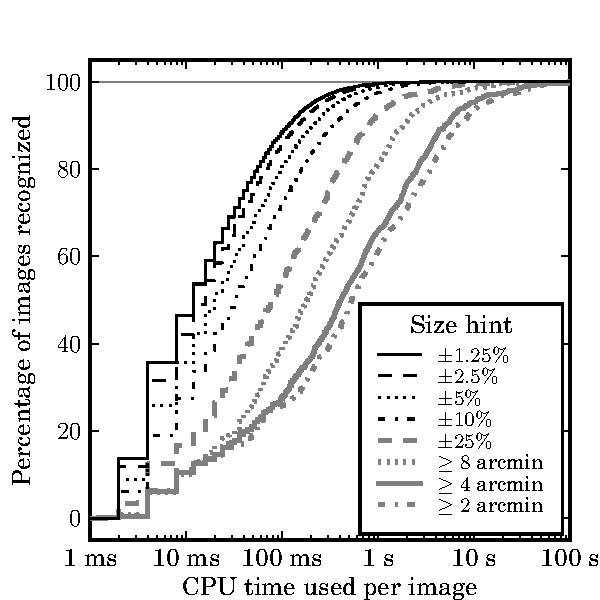
\includegraphics[width=1.000000\figunit]{sdss-sizehints-time}}
\newcommand{\sdsssizehintsindexfig}{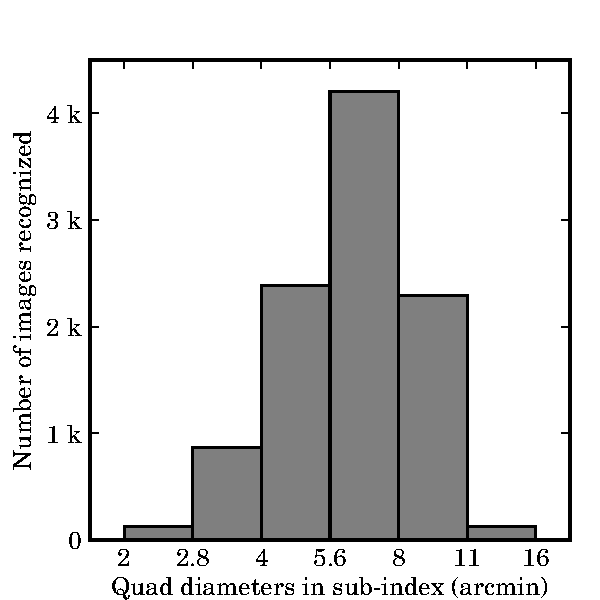
\includegraphics[width=1.000000\figunit]{sdss-sizehints-index}}
\newcommand{\sdssdensitytable}{\begin{tabular}{|c|D{.}{.}{3.2}|D{.}{.}{3.2}|D{.}{.}{3.2}|D{.}{.}{3.2}|D{.}{.}{3.2}|}
\hline
\multicolumn{1}{|c|}{\textbf{CPU time}} &\multicolumn{5}{c|}{\textbf{Percentage of images recognized}} \\
\cline{2-6}
\multicolumn{1}{|c|}{(per image)} & \multicolumn{1}{c|}{$16$ quads/cell} & \multicolumn{1}{c|}{$9$ quads/cell} & \multicolumn{1}{c|}{$4$ quads/cell} & \multicolumn{1}{c|}{$3$ quads/cell} & \multicolumn{1}{c|}{$2$ quads/cell} \\
\hline
\makebox[\pointonesec][r]{$0.1$ s} & 94.44  & 96.32  & 95.89  & 94.30  & 90.94 \\
\makebox[\pointonesec][r]{$1$ s} & 99.76  & 99.84  & 99.61  & 99.36  & 97.35 \\
\makebox[\pointonesec][r]{$10$ s} & 99.96  & 99.95  & 99.79  & 99.65  & 97.92 \\
\hline
\end{tabular}
}
\newcommand{\sdssdensityreltimefig}{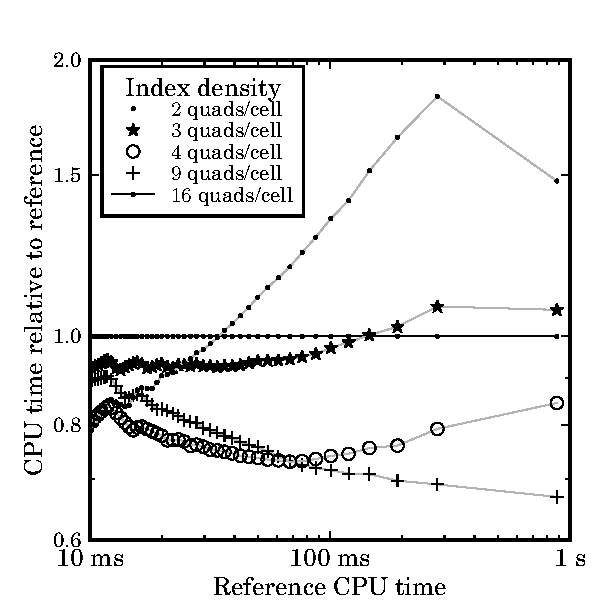
\includegraphics[width=1.000000\figunit]{sdss-density-reltime}}
\newcommand{\sdssdensitytimefig}{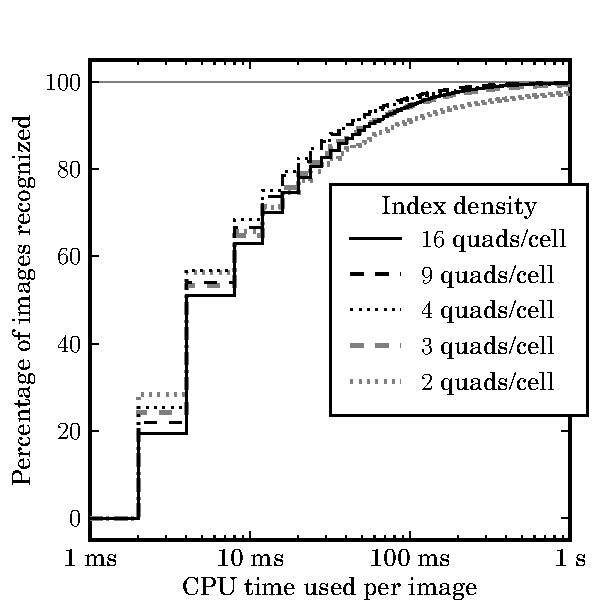
\includegraphics[width=1.000000\figunit]{sdss-density-time}}
\newcommand{\sdsstriquinttable}{\newlength{\cw}
\settowidth{\cw}{\textbf{Percentage of images recognized}}
\begin{tabular}{|c|D{.}{.}{3.2}|D{.}{.}{3.2}|D{.}{.}{3.2}|}
\hline
\multicolumn{1}{|c|}{\textbf{CPU time}} &\multicolumn{3}{c|}{\textbf{Percentage of images recognized}} \\
\cline{2-4}
\multicolumn{1}{|c|}{(per image)} & \multicolumn{1}{c|}{\makebox[0.35\cw][c]{Triangles}} & \multicolumn{1}{c|}{\makebox[0.35\cw][c]{Quads}} & \multicolumn{1}{c|}{\makebox[0.35\cw][c]{Quints}} \\
\hline
\makebox[\pointonesec][r]{$0.1$ s} & 0.20  & 57.45  & 23.35 \\
\makebox[\pointonesec][r]{$1$ s} & 28.07  & 92.20  & 36.67 \\
\makebox[\pointonesec][r]{$10$ s} & 78.58  & 99.28  & 72.75 \\
\makebox[\pointonesec][r]{$100$ s} & 99.15  & 99.33  & 95.08 \\
\makebox[\pointonesec][r]{$1000$ s} & 99.97  & 99.33  & 96.25 \\
\hline
\end{tabular}
}
\newcommand{\sdsstriquintntrynmatchfig}{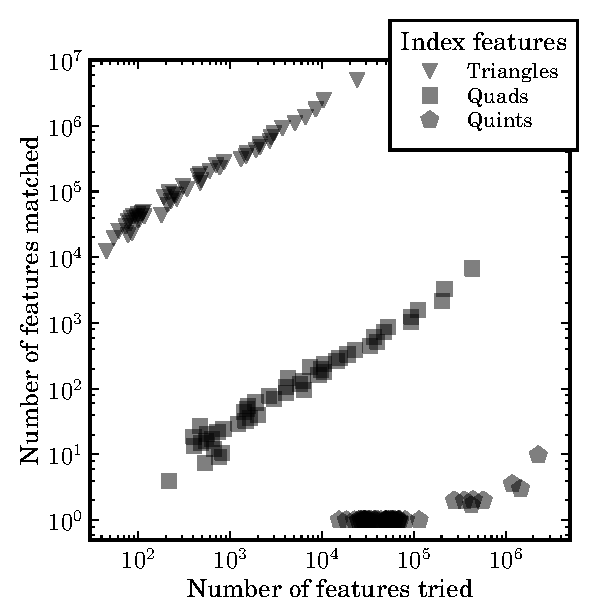
\includegraphics[width=1.000000\figunit]{sdss-triquint-ntrynmatch}}
\newcommand{\sdsstriquinttimefig}{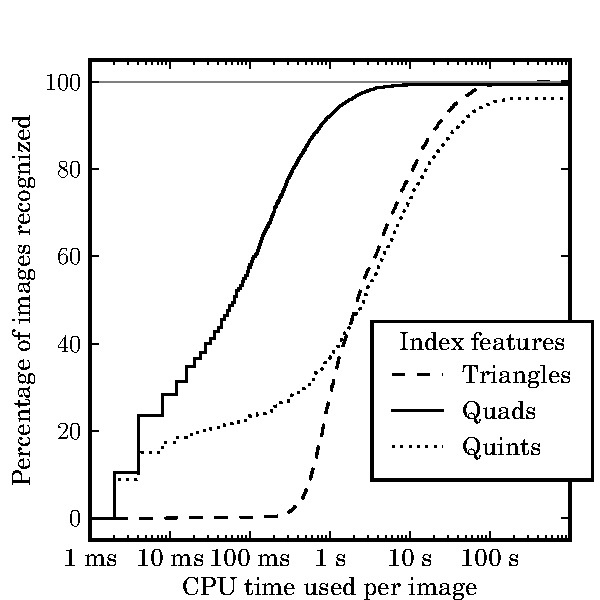
\includegraphics[width=1.000000\figunit]{sdss-triquint-time}}
\newcommand{\galextable}{\begin{tabular}{|c|D{.}{.}{3.2}|}
\hline
\multicolumn{1}{|c|}{\textbf{CPU time (per image)}} &\multicolumn{1}{c|}{\textbf{Percentage of images recognized}} \\
\hline
\makebox[\pointonesec][r]{$1$ s} & 74.46 \\
\makebox[\pointonesec][r]{$10$ s} & 93.56 \\
\makebox[\pointonesec][r]{$100$ s} & 98.95 \\
\makebox[\pointonesec][r]{$1000$ s} & 99.74 \\
\hline
\end{tabular}
}
\newcommand{\galexcputimefig}{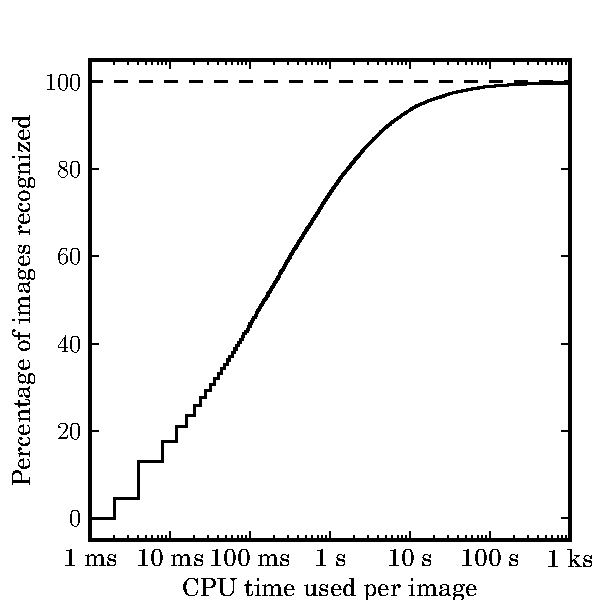
\includegraphics[width=1.000000\figunit]{galex-cputime}}
\newcommand{\galexindexidfig}{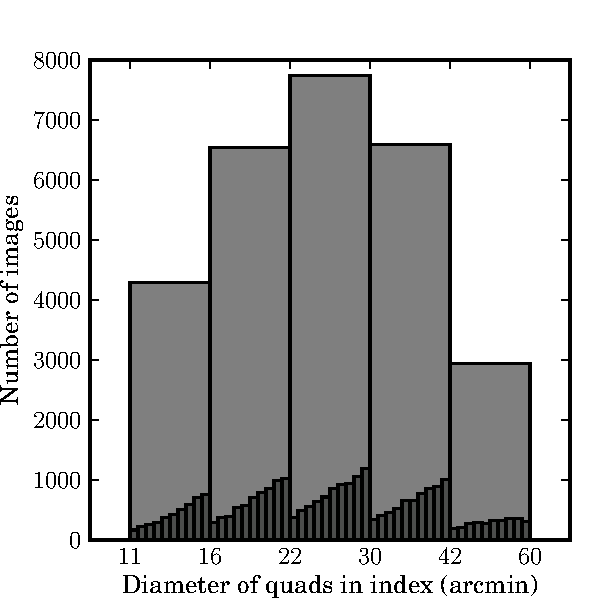
\includegraphics[width=1.000000\figunit]{galex-indexid}}
\newcommand{\galexquadfig}{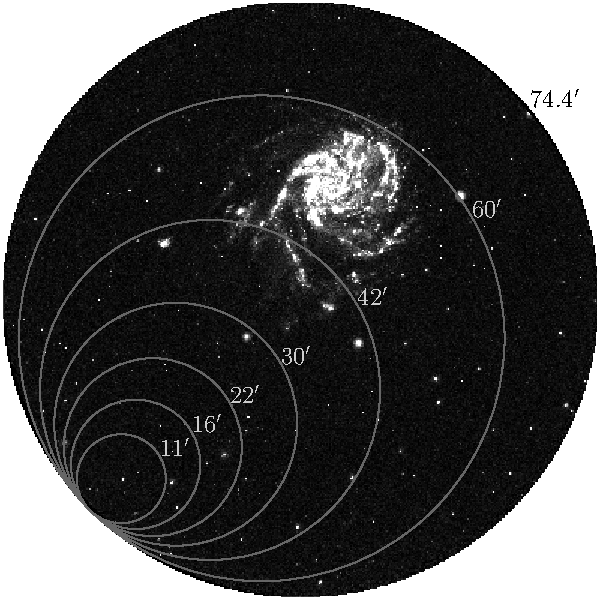
\includegraphics[width=1.000000\figunit]{galex-quad}}
\newcommand{\sdssquadfig}{\includegraphics[width=1.000000\figunit]{sdss-quad}}
\newcommand{\aegisacsquadfig}{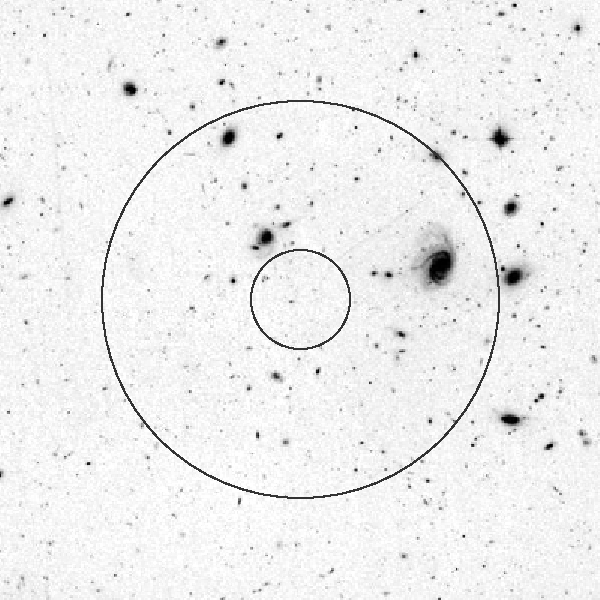
\includegraphics[width=1.000000\figunit]{aegis-acs-quad}}
\newcommand{\aegisacsquadsizesfig}{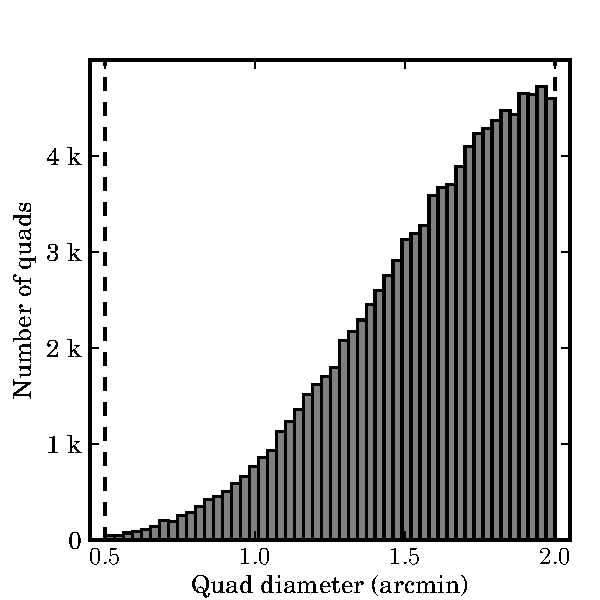
\includegraphics[width=1.000000\figunit]{aegis-acs-quadsizes}}


%%%% FIXMES ---

%%% --- move all acronym expansions and refs to the first time
%%%  they are used (2MASS, SDSS, GALEX / GR4/5, HST, SExtractor, AEGIS)

%% -- mention miserable failures

% Nice satellite hit on image and usnob:
%  http://live.astrometry.net/status.php?job=alpha-200904-31219616
%  http://trac.astrometry.net/attachment/wiki/MiserableFailures/fch1ILdbZ_ao0354.000.jpg
%  --> actually weird, that feature in USNOB isn't from the satellite, nor from the scratches
%    http://live.astrometry.net/status.php?job=alpha-200907-09480092
%    http://live.astrometry.net/status.php?job=alpha-200907-34435538
%  files are in sdss-tests/usnob-30.834--36.675-fchw6En7F_*

% Shooting star:
%   http://live.astrometry.net/status.php?job=alpha-200905-65967947
%   (76.064, -67.665)
%   usnob-76.064--67.665-fch4Pit7x_*.jpg
%   no source extraction: http://live.astrometry.net/status.php?job=alpha-200907-57428489
%  Test system: 
%   with old source extraction:
%    http://oven.cosmo.fas.nyu.edu/test/status.php?job=test-200908-97728064
%    (217.425 38.268), 6x4 degrees
%    defect is at (215.33, 38.50)
%    POSS-IE:272 and POSS-IO:272: ``National Geographic''



% ######## use this one ##########
% Shooting star 2:
%
% In alpha system:
%   http://live.astrometry.net/status.php?job=alpha-200905-71754521
%   (78.461, -7.832); 14 arcmin wide.
%   usnob-78.461--7.832-fchy7FiYt_sr0766*
%   -> usnob: calibration spots
%   tilerender -x 78.3 -X 78.6 -y -8.0 -Y -7.6 -w 512 -h 512 -l tycho -T tycho.mkdt.fits -l skdt -l userboundary -A fpargs -g 3 > out.png
%
% *****************************************************************
% Alpha system, with min size 0.25 deg:
%   http://live.astrometry.net/status.php?job=alpha-200909-12239075
%   (18.552, -7.529); 18.7 arcmin wide
%   usnob-18.552--7.529-fchxVG4d8
%   (calibration spots)
%   usnob-18.552--7.529-fch2zieuu_  with FITS
%   red band with calibration spot: sr0754
% *****************************************************************
%
% Alpha system, 19-30 arcmin:
%   (same as previous)
%   (18.552, -7.538); 19.6 arcmin wide
%   http://live.astrometry.net/status.php?job=alpha-200909-03279058
%
% Alpha system, 20-30 arcmin:
%   http://live.astrometry.net/status.php?job=alpha-200909-27760705
%   (106.519, -26.986); 20.9 arcmin wide
%   (bars on the plates)
%
% Alpha system, 21-30 arcmin:
%   (same as previous)
%   http://live.astrometry.net/status.php?job=alpha-200909-44695247
%   (106.467, -26.983); 27.4 arcmin wide
%
% Alpha system, with min size 0.5 deg:
%   (not great)
%   http://live.astrometry.net/status.php?job=alpha-200909-92156313
%   (210.279, 50.441); 1.36 deg wide.
%   usnob-210.279-50.441-fchikiRUi_s*
%   scratches (red) + National geographic (blue)
%   with --r2: usnob-210.279-50.441-fchUlLbML_so0175.000.jpg
%
% *************** use this one! ***********************************
% Alpha system, with min size 1.5 deg:
%   http://live.astrometry.net/status.php?job=alpha-200909-38045442
%   (163.396, 44.246); 2 deg wide.
%   usnob-163.396-44.246-fchf9tqUe_se0215*
%   National Geographic on one red plate
%   (POSS-IE, 103aE emulsion)
%   -> mosaic   (161.6-165.2, 43.0-45.5)
%   -> mosaic-c (162.75-165.25, 44.3)   -- top edge
%   -> mosaic-d (162.75, 43-44.3)       -- right edge
% *****************************************************************
%
% Alpha system, with min size 2.1 deg:
%   (nothing obvious)
%   http://live.astrometry.net/status.php?job=alpha-200909-10019626
%   (41.416, 9.845); 2.2 deg
%   usnob-41.416-9.845-fchoBp2G2_s*
%
% Alpha system, with min size 2.25 deg:
%   (97.458, 51.023); 2.33 deg
%   http://live.astrometry.net/status.php?job=alpha-200909-71452370
%   usnob-97.458-51.023-fchZEdtii*
%   (worms on red plate; plate edges aligned?)
%
% *****************************************************************
% Alpha system, with min size 2.35 deg:
%   (97.585, 51.012), 2.56 deg
%   http://live.astrometry.net/status.php?job=alpha-200909-67114974
%   (same as previous: worms on red plate; plate edges aligned?)
%   poss-ie, se0161
%   -> mosaic-e-*   (95.0-100.2, 49.5-52.6)
%   -> mosaic-f-*   (95.0-100.2, 51.0)   -- top edge
% *****************************************************************
%   
% Alpha system, with min size 2.6 deg:
%   (same as previous)
%   (97.975, 50.992), 2.93 deg
%   http://live.astrometry.net/status.php?job=alpha-200909-31052272

%
% In test system with alpha source extraction:
%   http://oven.cosmo.fas.nyu.edu/test/status.php?job=test-200908-80995437
%   (2.2x1.7 degrees wide)
%   usnob-250.964-14.869-fchN8erN6_*
%   http://edge.astrometry.net/gmaps?ra=250.9002685546875&dec=14.902321826141796&zoom=8&show=usnob,userOutline&userimage=test/200908/80995437&gain=2
%   POSS-IE:507 : ``National Geographic Society -- Palomar....'' underlining.


\comment{

SAM comments

1) Intro: for the thesis, looks great. But for journal submission,
think about if we want to start off with astronomical data / sharing?
or with the "here's an image, what's it of?" problem, which we special
case?  or with "data" --> "metadata" to enable search, cuz search is
the way?

2) "no false positives" -- we need to reword to something like "no
false positives caused by our system".

6)  end of 2.2; emphasize that in the "generate promising hypotheses
in a good order and check them" framework, there is no "right" number
of stars; it is just an empirical question about which search strategy
gets you to the answer fastest

11) for the table on p13:, can you expand the "phase" column into three:
Source Detections | Catalog | CPU Time per solve |
SDSS pipeline     | USNO B  | .1 s...;
SDSS | 2MASS | ?...;
astrometry.net | 2MASS | ?

13) conclusions, I think I agree with Hogg's comments here, and you
can be stronger about bragging!

-- "gallery" figures for Harvard, APOD, etc.

HOGG comments

Section 3.4:  Add a gallery of example images from the various test
sets; at least one amateur image, one astrophotograph, one archive
plate, one backyard photograph, etc.  This is a thesis, go to town!

Section 3.4:  Move the "Part of the remarkable..." discussion to the
discussion section.

Section 4:  De-scope and finish the discussion section.  Doesn't need
to be much for the thesis; we can re-scope it in HD when we prepare it
for submission to AJ.
}

\newcommand{\usnob}{USNO-B\xspace}
\newcommand{\twomass}{2MASS\xspace}
\newcommand{\USNOB}{USNO-B catalog\xspace}

\newcommand{\band}[1]{\ensuremath{#1}}
\newcommand{\uband}{\band{u}}
\newcommand{\gband}{\band{g}}
\newcommand{\rband}{\band{r}}
\newcommand{\iband}{\band{i}}
\newcommand{\zband}{\band{z}}

\section{Introduction}

% Things Hogg wanted in the intro:

% Heterogeneous and massive data
%  -LSST, SDSS, robotic networks
% VO
%  -trust model
%  -no model for calibration meta-data
% Internal vs external calibration
%  -SDSS ubercal
%  -blind date, photometric calibration/bandpass
% Image search
% Lost data
%  -SDSS
%  -amateurs
%  -plate archives
%  -rotting tape
%  -ground-based
% Existing systems
%  -SCAMP
%  -triangle-based
% What we have done
%  -huge search with geometric hashing
%  -goal-based indexing
%  -verification
%  -data structures, good engineering
%  -web interface, stand-alone code

% Add paragraph-to-paragraph glue.
%
% In the first paragraph:
%
% -give examples of things that can be got from "all" better than
% "one".
%
%  --time domain: variability (AAVSO?); GRB or SN precursors;
%    comets; proper motion
%
%  --cross-spectral: eg SDSS/GALEX
%
%  --space (quality) vs ground (quantity)
%
% -estimate the total size of the data set in pixels and in steradians
% and in Tb.
% 
%  -- The Sloan Digital Sky Survey (http://sdss.org/) contains about 4
% terapixels
%
%  -- The Palomar-Quest Sky Survey
% (http://www.astro.caltech.edu/\~{}george/pq/) is more than 10
% terapixels.
%
%  -- The Canada-Hawaii-France Legacy Survey
% (http://www.cfht.hawaii.edu/Science/CFHLS/) is 20 terapixels.
%
%  -- There are many more observatories and projects like these.
%
%  -- The Hubble Space Telescope (HST) archive
% (http://archive.stsci.edu/) is another few tens of terapixels.
%
%  -- The Digital Access to a Sky Century at Harvard historical
% plate-scanning project (http://hea-www.harvard.edu/DASCH/) has
% scanned over a terapixel so far and will produce over 150 terapixels
% in total.
%
%  -- The first phase of the PanSTARRS project
% (http://pan-starrs.ifa.hawaii.edu/public/) will produce more than
% 200 terapixels per year, and will exceed a petapixel per year in its
% final configuration.
%
%  -- The Large Synoptic Survey Telescope (http://www.lsst.org/) will
% produce a petapixel per year.

% thousands?

Although there are hundreds of ground- and space-based telescopes
currently operating, and petabytes of stored astronomical images (some
fraction of which are available in public archives), most astronomical
research is conducted using data from a single telescope.  Why do we
as astronomers limit ourselves to using only small subsets of the
enormous bulk of available data?  Three main reasons can be
identified: we don't want to share our data; it's hard to share our
data; and it's hard to use data that others have shared.  The latter
two problems can be addressed by technological solutions, and as
sharing data becomes easier, astronomers will likely become more
willing to do so.


% Galileo's anagram to Kepler about Saturn's rings
% http://www.mathpages.com/home/kmath151.htm

Historically, astronomical data---and, indeed, important scientific
results---have often been closely guarded.  In more recent times,
early access to data has been seen as one of the rewards for joining
and contributing to telescope-building collaborations, and proprietary
data periods typically accompany grants of observing time on
observatories such as the Hubble Space Telescope.  However, this seems
to be changing, albeit slowly.  One of the first large astronomical
data sets to be released publicly in a usable form was the Hubble Deep
Field \cite{hubbledeepfield}.  The Sloan Digital Sky Survey (SDSS)
\cite{sdsstechnical} is committed to yearly public data releases, 
and the members of upcoming projects such as the Large Synoptic Survey
Telescope (LSST) \cite{lsst} have recognized that the primary
advantage of contributing to the collaboration is not proprietary
access to the data, but rather a deep understanding and familiarity
with the telescope and data, and have (in principle) decided to make
the data available immediately.

% PanSTARRS: expect to release surveys ``after completion''

% The Hubble Wars: Astrophysics Meets Astropolitics in the Two-billion-dollar Struggle Over the Hubble Space Telescope
% By Eric Chaisson
% Published by Harvard University Press, 1998
% ISBN 0674412559, 9780674412552


Putting aside the issue of \emph{willingness} to share data, there are
issues of our \emph{ability} to share data effectively.  Making use of
large, heterogeneous, distributed image collections requires fast,
robust, automated tools for calibration, vetting, organization, search
and retrieval.


%\paragraph{A trust model for the Virtual Observatory.}

The Virtual Observatory (VO) \cite{vo} establishes a framework and
protocols for the organization, search, and retrieval of astronomical
images.  The VO is structured as a distributed system in which many
``publishers'' provide image collections and interfaces that allow
these images to be searched.  This distributed framework allows the VO
to scale, but it also means that any property we might want the images
published through the VO to have must be specified by the standards,
and we must trust all publishers to implement the standards correctly.
Of particular importance are calibration \metadata
\cite{astrometryandvo}.  The draft Simple Image Access Protocol
\cite{siap} states that ``an image should be a calibrated object
frame'' and specifies some loose requirements for astrometric
\metadata.  However, there is neither a requirement, nor a specified
method, for communicating more detailed information about the
calibration processes that have been applied to the image.  A VO user
who wants to know exactly how the raw CCD frame was reduced to the
pixel values in the image must use processes outside the VO
framework---most likely by reading papers and contacting the image
publisher---and this will take much longer than finding and retrieving
the image.


The VO cannot be expected to impose a minimum standard of ``quality''
on images published through VO protocols, for several reasons.  First,
doing so would require making a tradeoff between the quality and
quantity of images that are publishable.  Since different users of the
VO have different needs, there is no objective way to make this
tradeoff.  For example, one researcher might only want images taken
during photometric conditions, while one studying a transient event
might want all available imaging, regardless of quality.  Second,
there is no objective measure of the quality of an image: different
aspects of an image are important to different users.  Finally, even
the most well-intentioned and skilled publisher will occasionally make
mistakes, and this effect will become more pronounced as surveys
become more automated and data rates increase.  Thus, users of the VO
cannot in general rely on the quality or correctness of image data or
calibration \metadata, and individually hand-checking each image does
not scale to the future in which the VO provides access to any
significant fraction of the world's astronomical images.  For the
goals of the VO movement to be achieved, the tools that allow users to
vet, verify, and recalibrate images must be developed, and ideally
these tools will be integrated into the VO system.


In this \doctype we present a system, \an, that automatically
produces astrometric \metadata for astronomical images.  That is,
given an image, our system produces the pointing, scale, and
orientation of the image---the astrometric calibration \metadata or
World Coordinate System (WCS).  The system requires no first guess,
and works with the information in the image pixels alone.  The success
rate is above $99.9~\percent$ for contemporary near-ultraviolet and
visual imaging survey data, with no false positives.


%\paragraph{Lost data are found again.}

%FIXME!  Old tech report has good expanded paragraphs about
%  amateurs, etc


Our system enables an immense amount of ``lost'' astronomical imagery
to be used for scientific purposes.  This includes photographic plate
archives, an immense and growing number of images taken by amateur
astronomers, as well as data from individual professional astronomers
and ground-based observatories whose \metadata are non-existent,
lost, or simply wrong.  While many modern telescopes do produce
correct, standards-compliant \metadata, many others have control
systems that drift relative to the sky, yielding only approximate
astrometric \metadata.  Still others produce no \metadata, or produce
it in some ideosyncratic, non-standards-compliant form.  Even
sophisticated and highly-automated surveys such as SDSS occasionally
have failures in the systems that produce astrometric calibration
information, resulting in perfectly good but ``lost'' images.  A
system that makes these data available for study will effectively
recover a significant amount of lost observing time, fill in gaps in
the astronomical record, and make observers more productive by
eliminating the tedious and often unenlightening task of fixing the
astrometry.  Furthermore, a robust, fully-automated system allows the
data to be trusted, because the calibration \metadata, and their
associated error estimates, have been derived from the images
themselves, not from some unknown, undocumented, unverified or
untrustworthy external source.


%\paragraph{Image search.}

%---FIXME - don't mention photometric calibration if we don't talk
%about it in this paper... or mention that it is possible but not
%discussed here.


Our system can be seen as a specialized kind of image-based search.
Given an image, we can identify and label the objects that appear in
the image, with a very high success rate and no false positives.  We
have achieved the ultimate goal of computer vision, within the domain
of astronomical images.  Our system is based solely on the contents of
the image, in sharp contrast to most contemporary image search systems
(such as Google Image Search), which rely on contextual
information---the text surrounding the image on a web page---rather
than the information in the image itself.


% Only possible because astro images are relatively simple

%\paragraph{Prior work.}


In the literature, the task of recognizing astronomical images is
known as ``blind astrometric calibration'' or the ``lost in space''
problem, since an early application was for estimating the attitude of
a spacecraft using a camera mounted on the spacecraft.  By identifying
the stars that are visible, the pose of the camera can be determined
\cite{liebe1993}.  In such systems, triangles of stars are typically
used as geometric features (e.g. \cite{junkins1977}).  Triangles are
effective in this regime because the images typically span tens of
degrees and contain only dozens of very bright stars: the search space
is small.  Furthermore, these systems are not fully ``blind'' in that
they are designed for particular cameras, the specifications of which
are available to the system designers.


Triangle-based approaches have also been used to fine-tune the astrometry
problem when a good initial estimate is available \cite{pal2006}.
Because the search domain is limited to a small area around the
initial estimate, the triangle-based approach is effective.
Completely blind systems have been attempted previously (for example,
\cite{harvey2004} and references therein) but none we know of have been
able to achieve the scalability and fidelity of our approach.


Both the triangle matching approach and ours (described below) are
based on ``geometric hashing'' (for example, \cite{lamdan1990},
\cite{huttenlocher1990}).  Our system uses the same two-step
approach used by these systems, in which a set of hypotheses are
generated from sparse matches, then a second stage does detailed
verification of the hypotheses.


There are several automated calibration systems that refine the
astrometric calibration of an image to produce a high-precision
alignment to a reference catalog given a good first guess (for
example, \cite{valdes1995, wcstools4, bertin2005}).  These systems are
reliable and robust, but they require a reasonable first guess about
the image pointing, orientation, and scale.  Our system can be used to
\emph{create} that good first guess.


% Talk about what we assume -- TAN projection, small distortion,
% square pixels


\section{Methods}

%% FIXME - get the ``quad'', ``triangle'', ``quintuple'' terminology
%% straight.  ``asterism''?  ``feature''?

% ``query'', ``index''

% ``index stars'', ``index quads'' vs ``reference stars'', ``referenc catalog''

Our approach involves four main components.  First, when given a query
image, we detect astronomical sources (``stars'', hereafter) by
running a number of image-processing steps.  This typically yields a
few hundred or more stars localized to sub-pixel accuracy.  Next, the
system examines subsets of these stars, producing for each subset a
geometric hash code that describes their relative positions.  We
typically use subsets of four stars, which we call ``quads.''  Having
computed the hash code for the query quad, the system then searches in
a large pre-computed index for almost identical hash codes.  Each
matching hash code that is found corresponds to a hypothesized
alignment between the quad in the query image and the quad in the
index, which can be expressed as a hypothesized location, scale, and
orientation of the image on the sky.  The final component is a
verification criterion, phrased as a Bayesian decision problem, which
can very accurately decide if the hypothesized alignment is correct.
The system continues generating and testing hypotheses until we find
one that is accepted by the verification process; we then output that
hypothesis as our chosen alignment.  In some cases, we never find a
hypothesis in which we are sufficiently confident (or we give up
searching before we find one), but our thresholds are set
conservatively enough that we almost never produce a false positive
match.  Each component of our approach is outlined below.

%--- where should this paragraph go?

The primary technical contributions of our system include the use of
the ``geometric hashing'' \cite{lamdan1990, wolfson1997} approach to
solve the huge search problem of generating candidate calibrations; an
index-building strategy that takes into account the distribution of
images we wish to calibrate; the verification procedure which
determines whether a proposed astrometric calibration is correct; and
good software engineering which has allowed us to produce a practical,
efficient system.  All our code is publicly available under the GPL
license, and we are also offering a web service.


\subsection{Star detection}

The system automatically detects compact objects in each input image
and centroids them to yield the pixel-space locations of stars.  This
problem is an old one in astronomy; the challenge \emph{here} is to
perform it robustly, with no human intervention, on the large variety
of input images the system faces.  Luckily, because the rest of the
system is so robust, it can handle detection lists that are missing a
few stars or have some contaminants.

The first task is to identify (detect) localized sources of light in
the image.  Most astronomical images exhibit sky variations,
sensitivity variations, and scattering; we need to find peaks on top
of such variations.  First we subtract off a median-smoothed version
of the image to ``flatten'' it.  Next, to find statistically
significant peaks, we need to know the approximate noise level.  We
find this by choosing a few thousand random pairs of pixels separated
by five rows and columns, calculating the difference in the fluxes for
each pair, and calculating the variance of those differences, which is
approximately twice the variance $\sigma^2$ in each pixel.  At this
point, we identify pixels which have values in the flattened image
that are $>8\,\sigma$, and connect detected pixels into individual
detected objects.

The second task is to find the peak or peaks in each detected object.
This determination begins by identifying pixels that contain larger
values than all of their neighbors.  However, keeping all such pixels
would retain peaks that are just due to uncorrelated noise in the
image and individual peaks within a single ``object.''  To clean the
peak list, we look for peaks that are joined to smaller peaks by
saddle points within $3\,\sigma$ of the larger peak (or $1~\percent$
of the larger peak's value, whichever is greater), and trim the
smaller peaks out of our list.

%%%% FIXME -- what does the code actually do?

Finally, given the list of all peaks, the third task is to centroid
the star position at sub-pixel accuracy. Following previous work
\cite{sdssimaging}, we take a $3\times 3$ grid around each star's peak
pixel, effectively fitting a Gaussian model to the nine values, and
using the peak of the Gaussian. Occasionally this procedure produces a
Gaussian peak outside the $3\times 3$ grid, in which case we default
to the peak pixel, although such cases are virtually always caused by
image artifacts.  This procedure produces a set of $x$ and $y$
positions in pixel coordinates corresponding to the position of
objects in the image.

% Mention more sophisticated options -- modelling the PSF and fitting
% that rather than the rather arbitrary Gaussian -- (which isn't what
% it actually does anyway!  It fits a general paraboloid!)

Compared to other star detection systems such as
SExtractor \cite{sextractor}, our approach is simpler and generally
more robust given a wide variety of images and no human intervention.
For example, while we do a simple median-filtering to remove the
background signal from the image, SExtractor uses sigma-clipping and
mode estimation on a grid of subimages, which are then median-filtered
and spline-interpolated.

\subsection{Hashing of asterisms to generate hypotheses}

Hypotheses about the location of an astronomical image live in the
continuous four-dimensional space of position on the celestial sphere
(pointing of the camera's optical axis), orientation (rotation of the
camera around its axis), and field of view (solid angle subtended by
the camera image).  We want to be able to recognize images that span
less than one-millionth the area of the sky, so the effective number
of hypotheses is large; exhaustive search will be impractical.  We
need a fast search heuristic: a method for proposing hypotheses that
almost always proposes a correct hypothesis early enough that we have
the resources to discover it.

\begin{figure}[htp]
  \begin{center}
    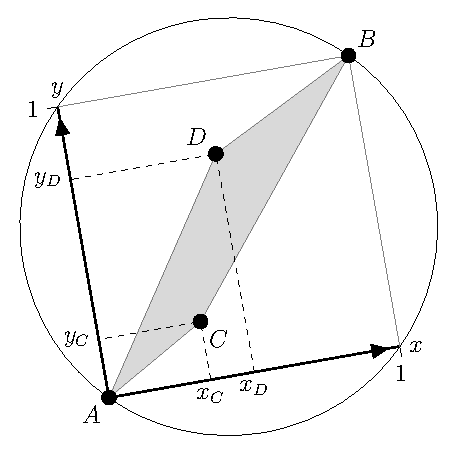
\includegraphics[width=\quadfigwidth]{quad-fig}
  \end{center} 
  \caption{The geometric hash code for a ``quad'' of stars, $\starA$,
      $\starB$, $\starC$, and $\starD$.  Stars $\starA$ and $\starB$
      define the origin and \mbox{$(1,1)$,} respectively, of a local
      coordinate system, in which the positions of stars $\starC$ and
      $\starD$ are computed.  The
      coordinates \mbox{$(\xC,\yC,\xD,\yD)$} become our geometric hash
      code that describes the relative positions of the four stars.
	  The hash code is invariant under translation, scaling, and
      rotation of the four stars.  \label{fig:quad}}
\end{figure}


Our fast search heuristic uses a continuous geometric hashing
approach.  Given a set of stars (a ``quad''), we compute a local
description of the shape---a geometric hash code---by mapping the
relative positions of the stars in the quad into a point in a
continuous-valued, 4-dimensional vector space (``code space'').
\Figref{fig:quad} shows this process.  Of the four stars comprising
the quad, the most widely-separated pair are used to define a local
coordinate system, and the positions of the remaining two stars in
this coordinate system serve as the hash code.  We label the most
widely-separated pair of stars ``$\starA$'' and ``$\starB$''.  These
two stars define a local coordinate system.  The remaining two stars
are called ``$\starC$'' and ``$\starD$'', and their positions in this
local coordinate system are $(\xC,\yC)$ and $(\xD,\yD)$.  The
geometric hash code is simply the 4-vector \mbox{$(\xC,\yC,\xD,\yD)$}.
We require stars $\starC$ and $\starD$ to be within the circle that
has stars $\starA$ and $\starB$ on its diameter.  This hash code has
some symmetries: swapping $\starA$ and $\starB$ converts the code to
\mbox{$(1\!-\!\xC,1\!-\!\yC,1\!-\!\xD,1\!-\!\yD)$} while swapping
$\starC$ and $\starD$ converts \mbox{$(\xC,\yC,\xD,\yD)$} into
\mbox{$(\xD,\yD,\xC,\yC)$.}  In practice, we break this symmetry by
demanding that \mbox{$\xC \le \xD$} and that \mbox{$\xC + \xD \le 1$;}
we consider only the permutation (or relabelling) of stars that
satisfies these conditions (within noise tolerance).


This mapping has several properties that make it well suited to our
indexing application. First, the code vector is \emph{invariant} to
translation, rotation and scaling of the star positions so that it can
be computed using only the relative positions of the four stars in any
conformal coordinate system (including pixel coordinates in a query
image).  Second, the mapping is \emph{smooth}: small changes in the
relative positions of any of the stars result in small changes to the
components of the code vector; this makes the codes resilient to small
amounts of positional noise in star positions.  Third, if stars are
uniformly distributed on the sky (at the angular scale of the quads
being indexed), codes will be uniformly distributed in (and thus make
good use of) the 4-dimensional code-space volume.


Noise in the image and distortion caused by the atmosphere and
telescope optics lead to noise in the measured positions of stars in
the image.  In general this noise causes the stars in a quad to move
slightly with respect to each other, which yields small changes in the
hash code (\ie, position in code space) of the quad.  Therefore, we
must always match the image hash code with a \emph{neighborhood} of
hash codes in the index.


The standard geometric hashing ``recipe'' would suggest using
triangles rather than quads.  However, the positional noise level in
typical astronomical images is sufficiently high that triangles are
not distinctive enough to yield reasonable performance.  An important
factor in the performance of geometric hashing system is the
``oversubscription factor'' of code space.  The number of hash codes
that must be contained in an index is determined by the effective
number of objects that are to be recognized by the system: if the goal
is to recognize a million distinct objects, the index must contain at
least a million hash codes.  Each hash code effectively occupies a
volume in code space: since hash codes can vary slightly due to
positional noise in the inputs (star positions), we must always search
for matching codes within a volume of code space.  This volume is
determined by the positional noise levels in the input image and the
reference catalog.  The oversubscription factor of code space, if it
is uniformly populated, is simply the number of codes in the index
multiplied by the fractional volume of code space occupied by each
code.  If triangles are used, the fractional volume of code space
occupied by a single code is large, so the code space becomes heavily
oversubscribed.  Any query will match many codes by coincidence, and
the system will have to reject all of these false matches, which is
computationally expensive.  By using quads instead of triangles, we
nearly \emph{square} the distinctiveness of our features: a quad can
be thought of as two triangles that share a common edge, so a quad
essentially describes the co-occurrence of two triangles.  A much
smaller fraction of code space is occupied by each quad, so we expect
fewer coincidental (false) matches for any given query, and therefore
fewer false hypotheses which must be rejected.


We could use quintuples of stars, which are even more distinctive than
quads.  However, there are two disadvantages to increasing the number
of stars in our asterisms.  The first is that the probability that all
$k$ of the stars in an indexed asterism appear in the image and that
all $k$ of the stars in a query asterism appear in the index both
decrease with increasing $k$.  For images taken at wavelengths far
from the catalog wavelength, or shallow images, this consideration can
become severe.  The second disadvantage is that near-neighbor lookup,
even with a \kdtree, becomes more time-consuming with increasing
dimensionality. The dimensionality of the code space for quintuples is
$6$-dimensional, compared to the $4$-dimensional code space of quads.
We test triangle- and quintuple-based indices in
\secref{sec:triquint} below.


When presented with a list of stars from an image to calibrate, the
system iterates through groups of four stars, treating each group as a
quad and computing its hash code.  Using the computed code, we perform
a neighborhood lookup in the index, retrieving all the indexed codes
that are close to the query code, along with their corresponding
locations on the sky.  Each retrieved code is effectively a
\emph{hypothesis}, which proposes to identify the four reference
catalog stars used to create the code at indexing time with the four
stars used to compute the query code. Each such hypothesis is
evaluated as described below.


The question of which hypotheses to check and when to check them is a
purely heuristic one. One could chose to wait until a hypothesis has
two or more ``votes'' from independent codes before checking it or
check every hypothesis as soon as it is proposed, whichever is faster.
In our experiments, we find that it is faster, and much less
memory-intensive, to simply check every hypothesis rather than
accumulate votes.


\subsection{Indexing the sky}


As with all geometric hashing systems, our system is based around a
pre-computed index of known asterisms.  Building the index begins with
a reference catalog of stars.  We typically use an all-sky (or
near-all-sky) optical survey such as USNO-B1 \cite{usnob,
barroncleaning} as our reference catalog, but we have also used the
infrared 2MASS catalog \cite{twomass} and the ultraviolet catalog from
GALEX \cite{galex}, as well as non-all-sky catalogs such as SDSS.
From the reference catalog we select a large number of quads (using a
process described below).  For each quad, we store its hash code and a
reference to the four stars of which it is composed.  We also store
the positions of those four stars.  Given a query quad, we compute its
hash code and search for nearby codes in the index.  For each nearby
code, we look up the corresponding four stars in the index, and create
the hypothesis that the four stars in the query quad correspond to the
four stars in the index.  By looking up the positions of the query
stars in image coordinates and the index stars in celestial
coordinates, we can express the hypothesis as a pointing, scale, and
rotation of the image on the sky.


In order for our approach to be successful, our index must balance
several properties.  We want to be able to recognize images from any
part of the sky, so we want to choose quads uniformly over the sky.
We want to be able to recognize images with a wide range of angular
sizes, so we want to choose quads of a variety of sizes.  We expect
that brighter stars will be more likely to be found in our query
images, so we want to build quads out of bright stars preferentially.
However, we also expect that some stars, even the brightest stars,
will be missing or mis-detected in the query image (or the reference
catalog), so we want to avoid over-using any particular star to build
quads.


We handle the wide range of angular sizes by building a series of
sub-indices, each of which contains quads whose quads have scales
within a small range (for example, a factor of two).  At some level
this is simply an implementation detail: we could recombine the
sub-indices into a single index, but in what follows it is helpful to
be able to assume that the sub-index will be asked to recognize query
images whose angular sizes are similar to the size of the quads it
contains.  Since we have a set of sub-indices, each of which is tuned
to an overlapping range of scales, we know that at least one will be
tuned to the scale of the query image.

\begin{figure}[htp]
\begin{center}
% This and the following figs are generated by sdss-tests/cut-index-fig.sh
%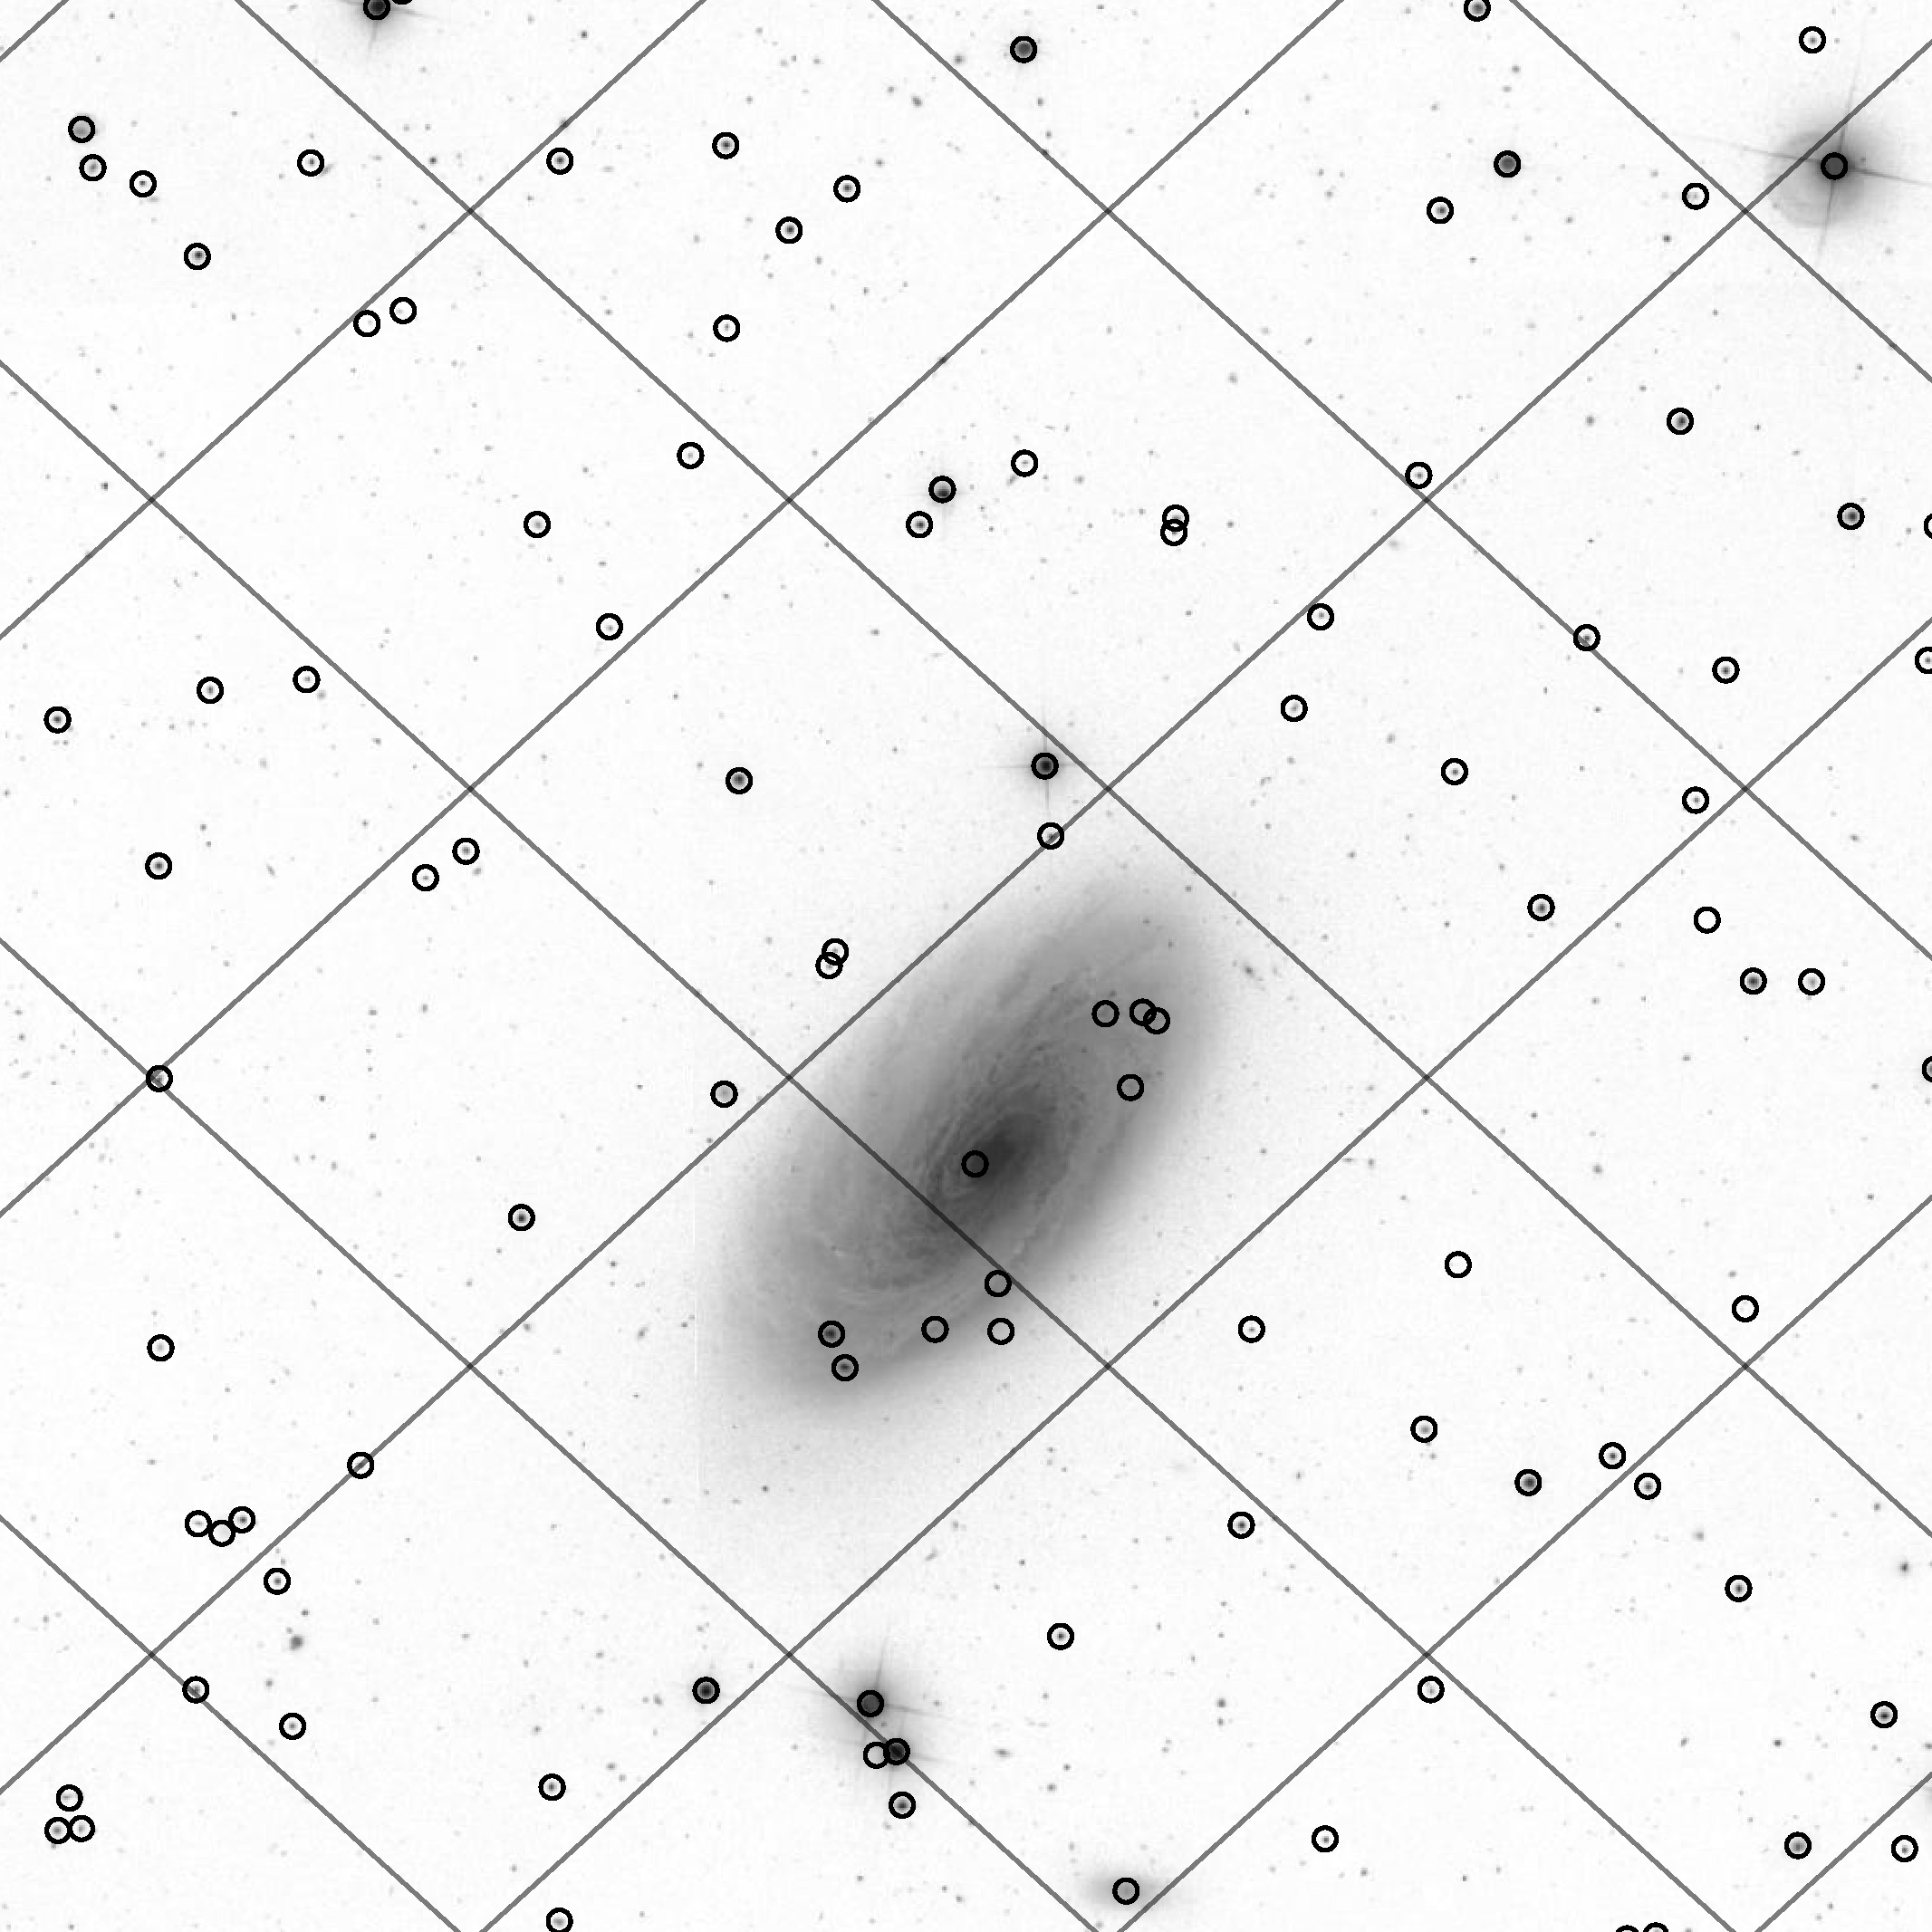
\includegraphics[width=\textwidth]{cut}
\setlength{\fboxsep}{0.5pt}
\framebox{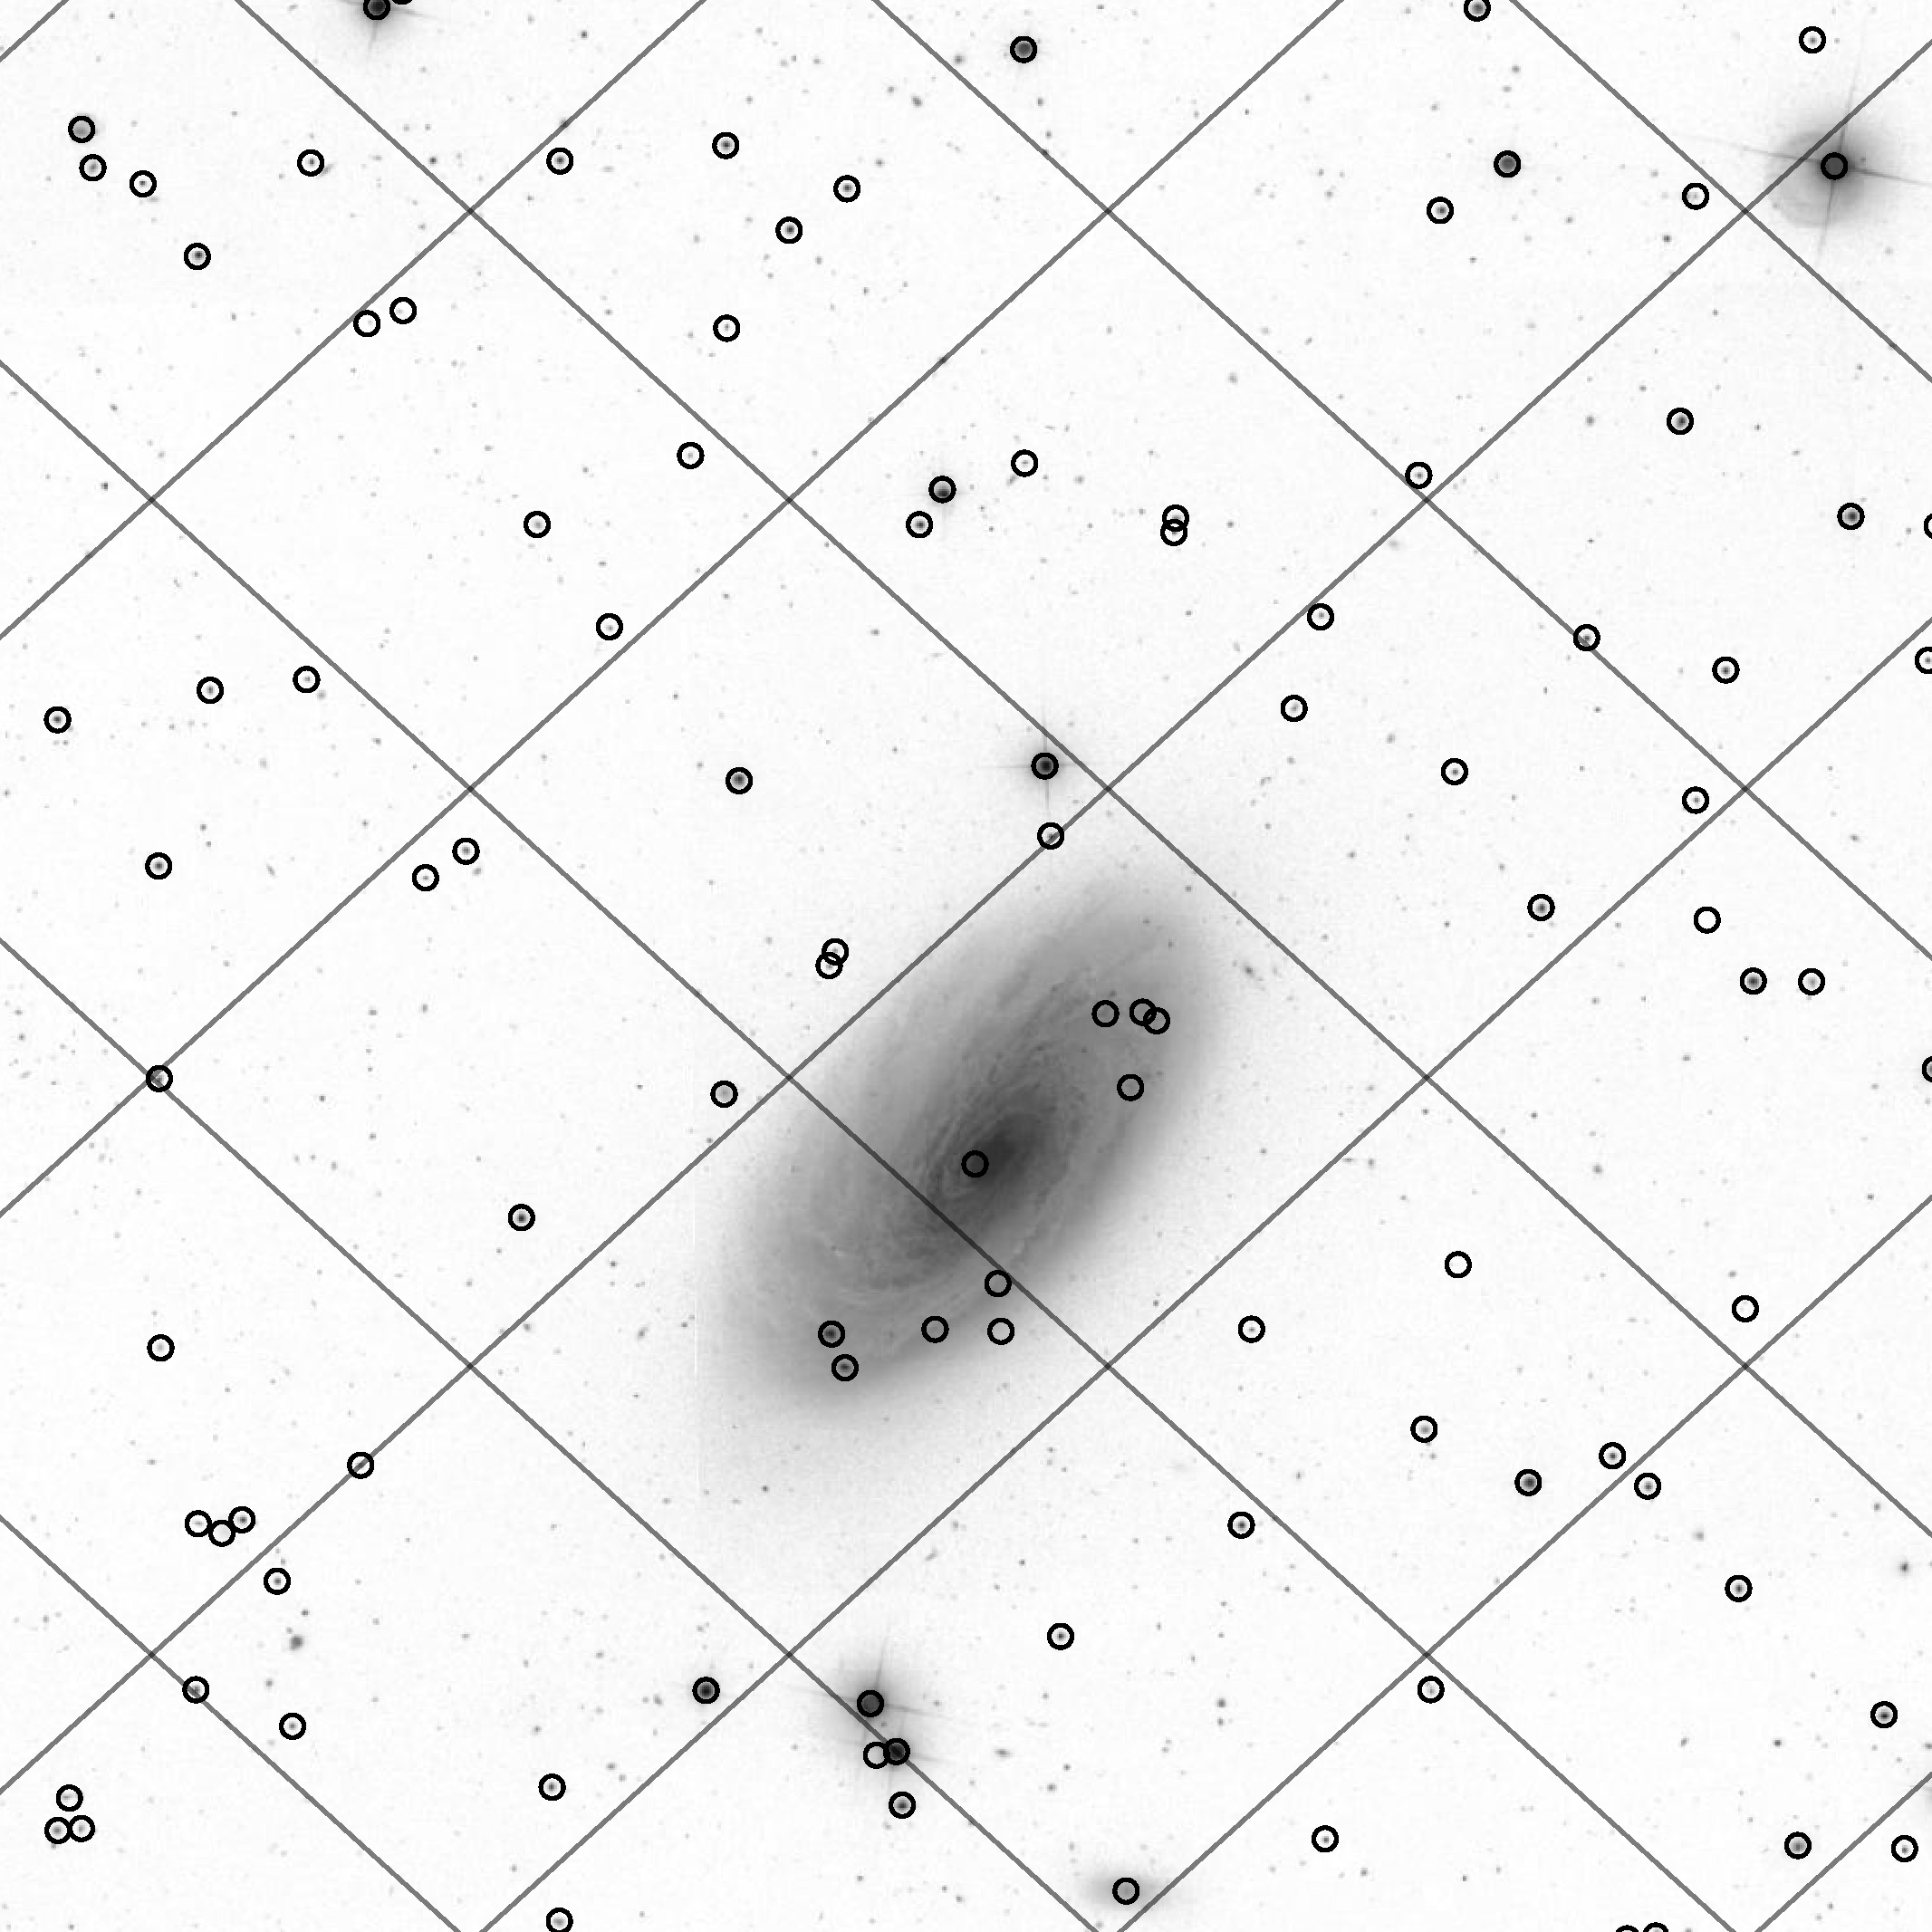
\includegraphics[width=0.99\textwidth]{cut}}
\end{center}
\caption{A small region of sky (about $0.3\times0.3~\degrees$ centered on
$(\RA, \Dec) = (188, 14.45)~\degrees$), showing the \healpix grid, and the
brightest $5$ stars that we select from each cell.  The image
shown is from the Sloan Digital Sky Survey.
\label{fig:cut}}
\end{figure}

We begin by selecting a spatially-uniform and bright subset of stars
from our reference catalog.  We do this by placing a grid of
equal-area patches (``HEALPixels'' \cite{healpix}) over the sky and
selecting a fixed number of stars, ordered by brightness, from each
grid cell.  The grid size is chosen so that grid cells are a small
factor smaller than the query images.  Typically we choose the grid
cells to be about a third of the size of the query images, and select
$10$ stars from each grid cell, so that most query images will contain
about a hundred query stars.  \Figref{fig:cut} illustrates this
process on a small patch of sky.


\begin{figure}[htp]
\begin{center}
%\includegraphics[width=\textwidth]{quads1}
\setlength{\fboxsep}{0.5pt}
\framebox{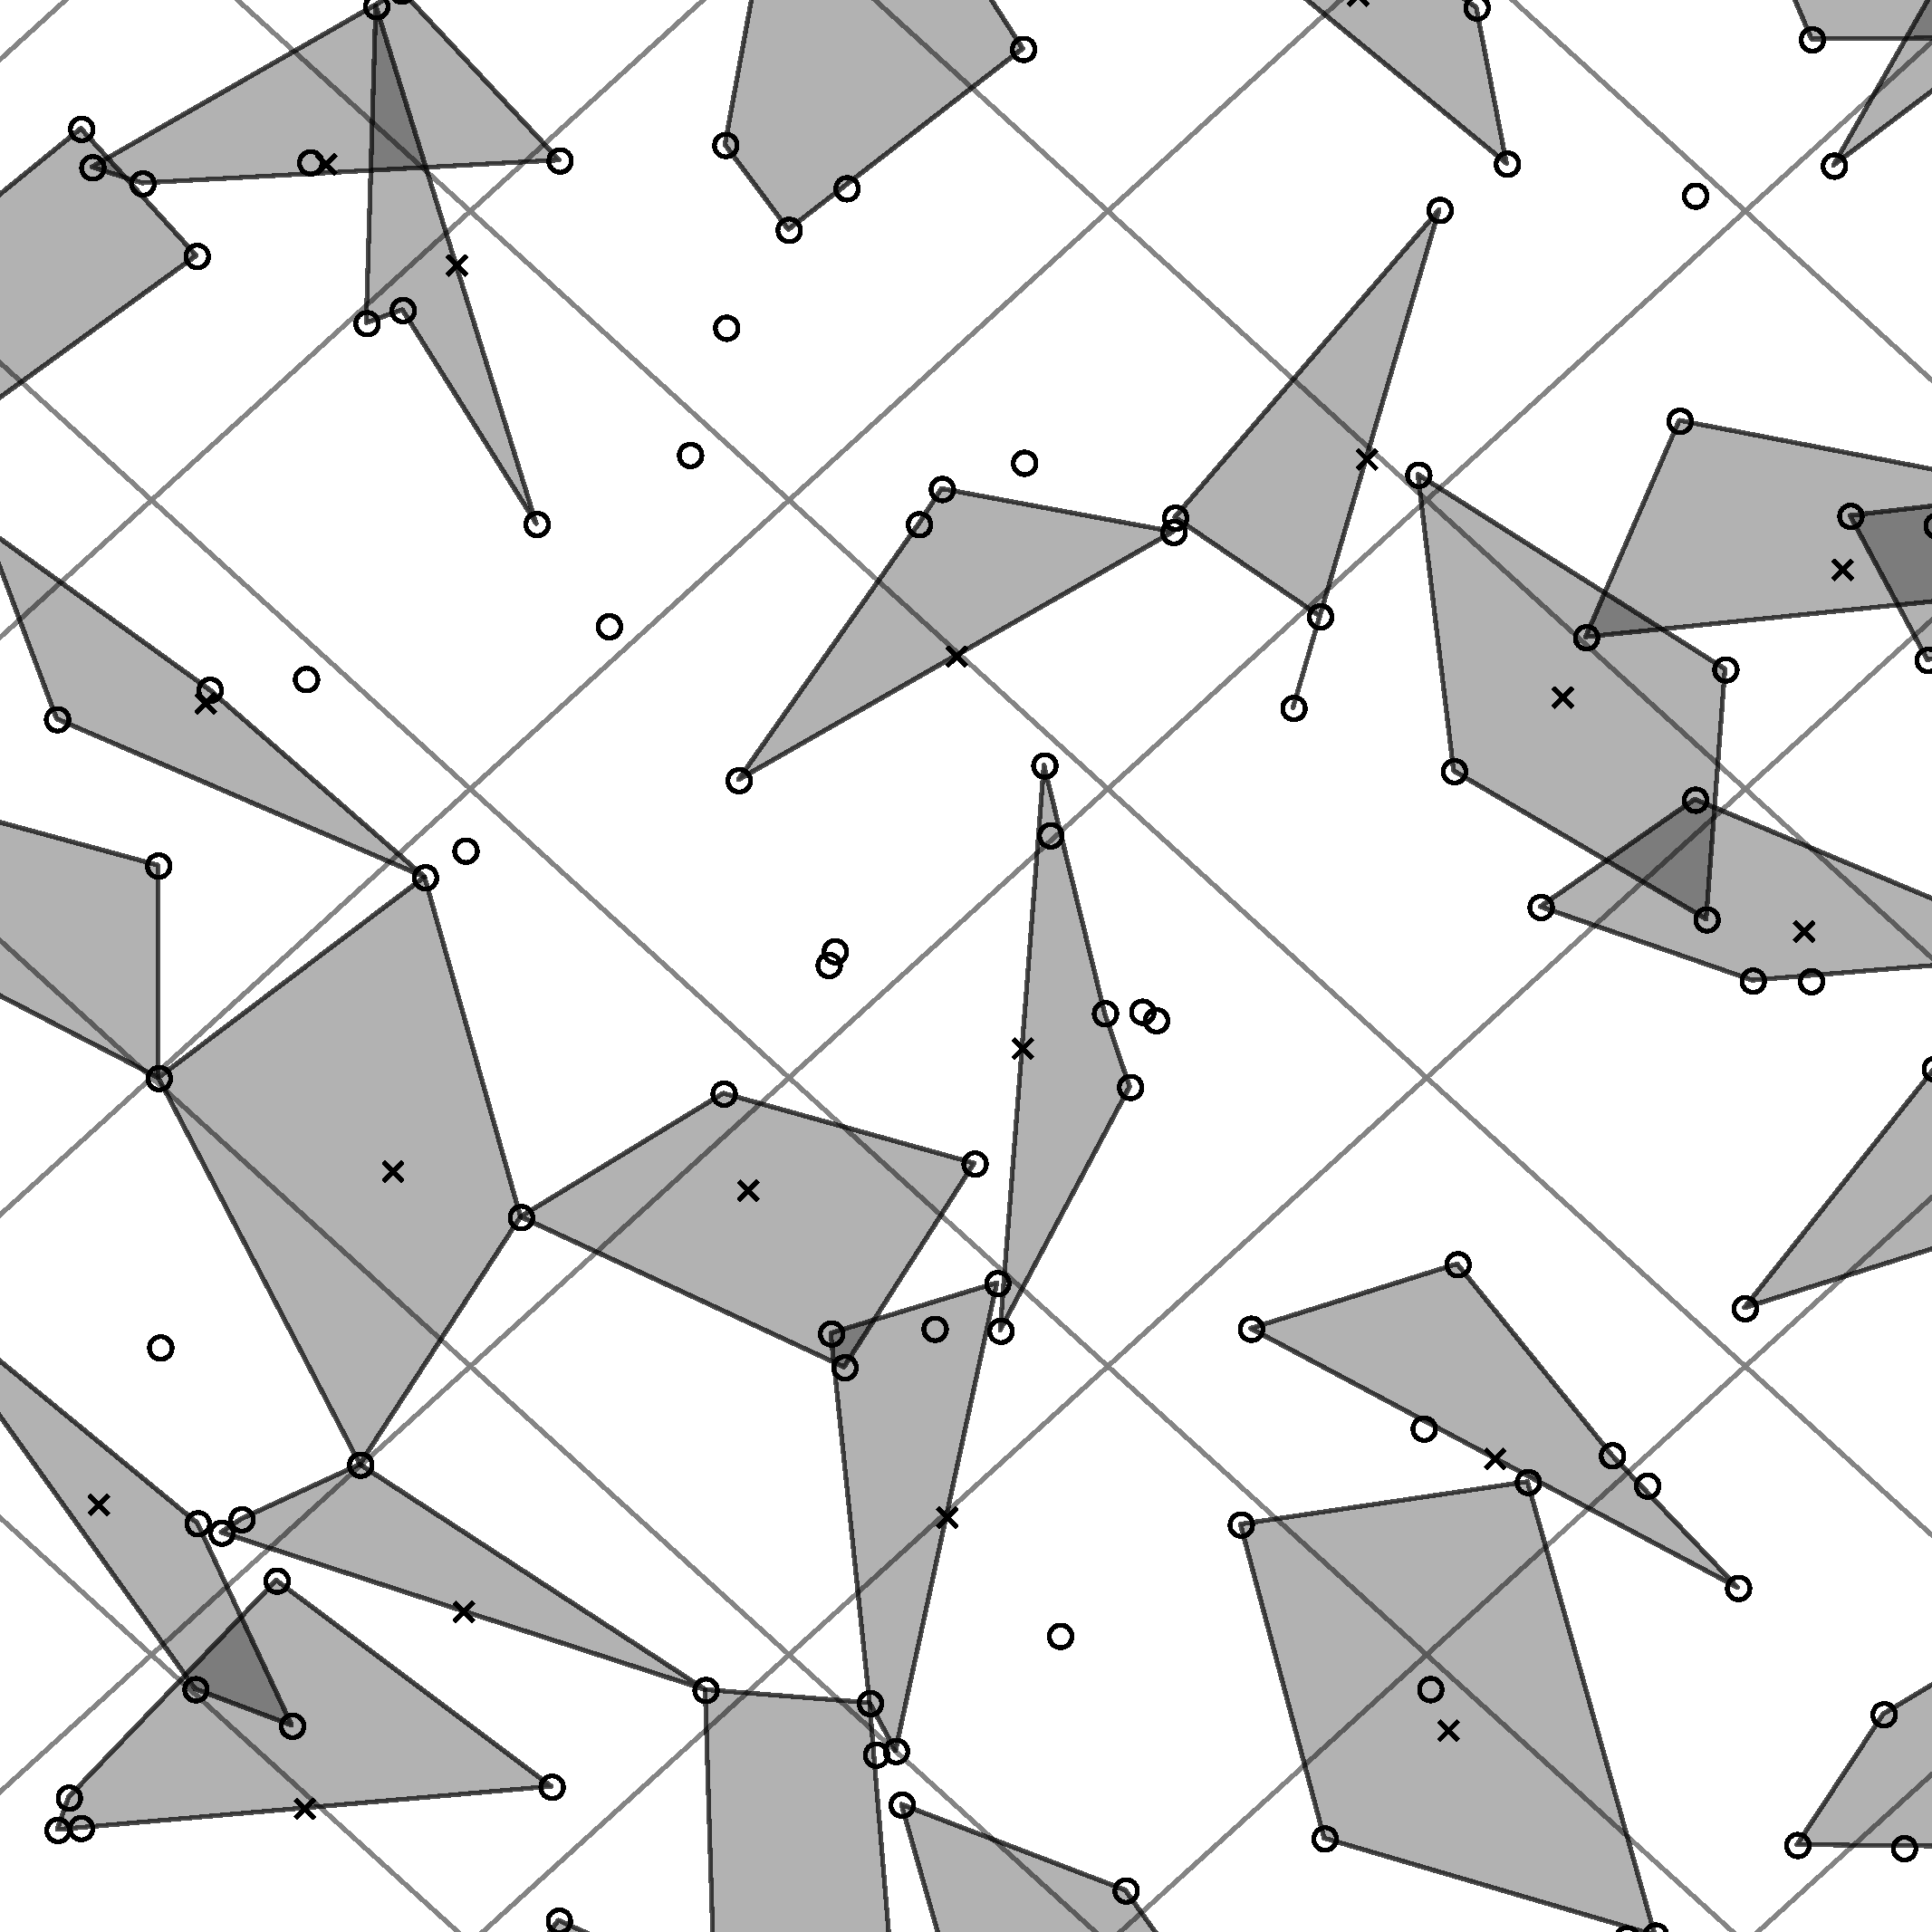
\includegraphics[width=0.99\textwidth]{quads1b}}
\end{center}
\caption{The same region of sky as shown in the previous figure, showing the
\healpix grid, and the quads that are created during the first pass through
the grid cells.  The quads must have a diameter (the distance between
the two most distant stars) within a given range---in this case, $1$
to $\sqrt{2}$ times the side-length of the grid cells.  In each grid
cell, the system attempts to build a quad whose center (\ie, midpoint
of the diameter line)---marked with an $\mathbf{\times}$ in the
figure---is within the grid cell.
\label{fig:quad1}}
\end{figure}

%% FIXME - shrink ``quads2'' and add ``quads4'' side-by-side ?
%% -mark 'X'es too

\begin{figure}[htp]
\begin{center}
%\includegraphics[width=\textwidth]{quads2}
\setlength{\fboxsep}{0.5pt}
\framebox{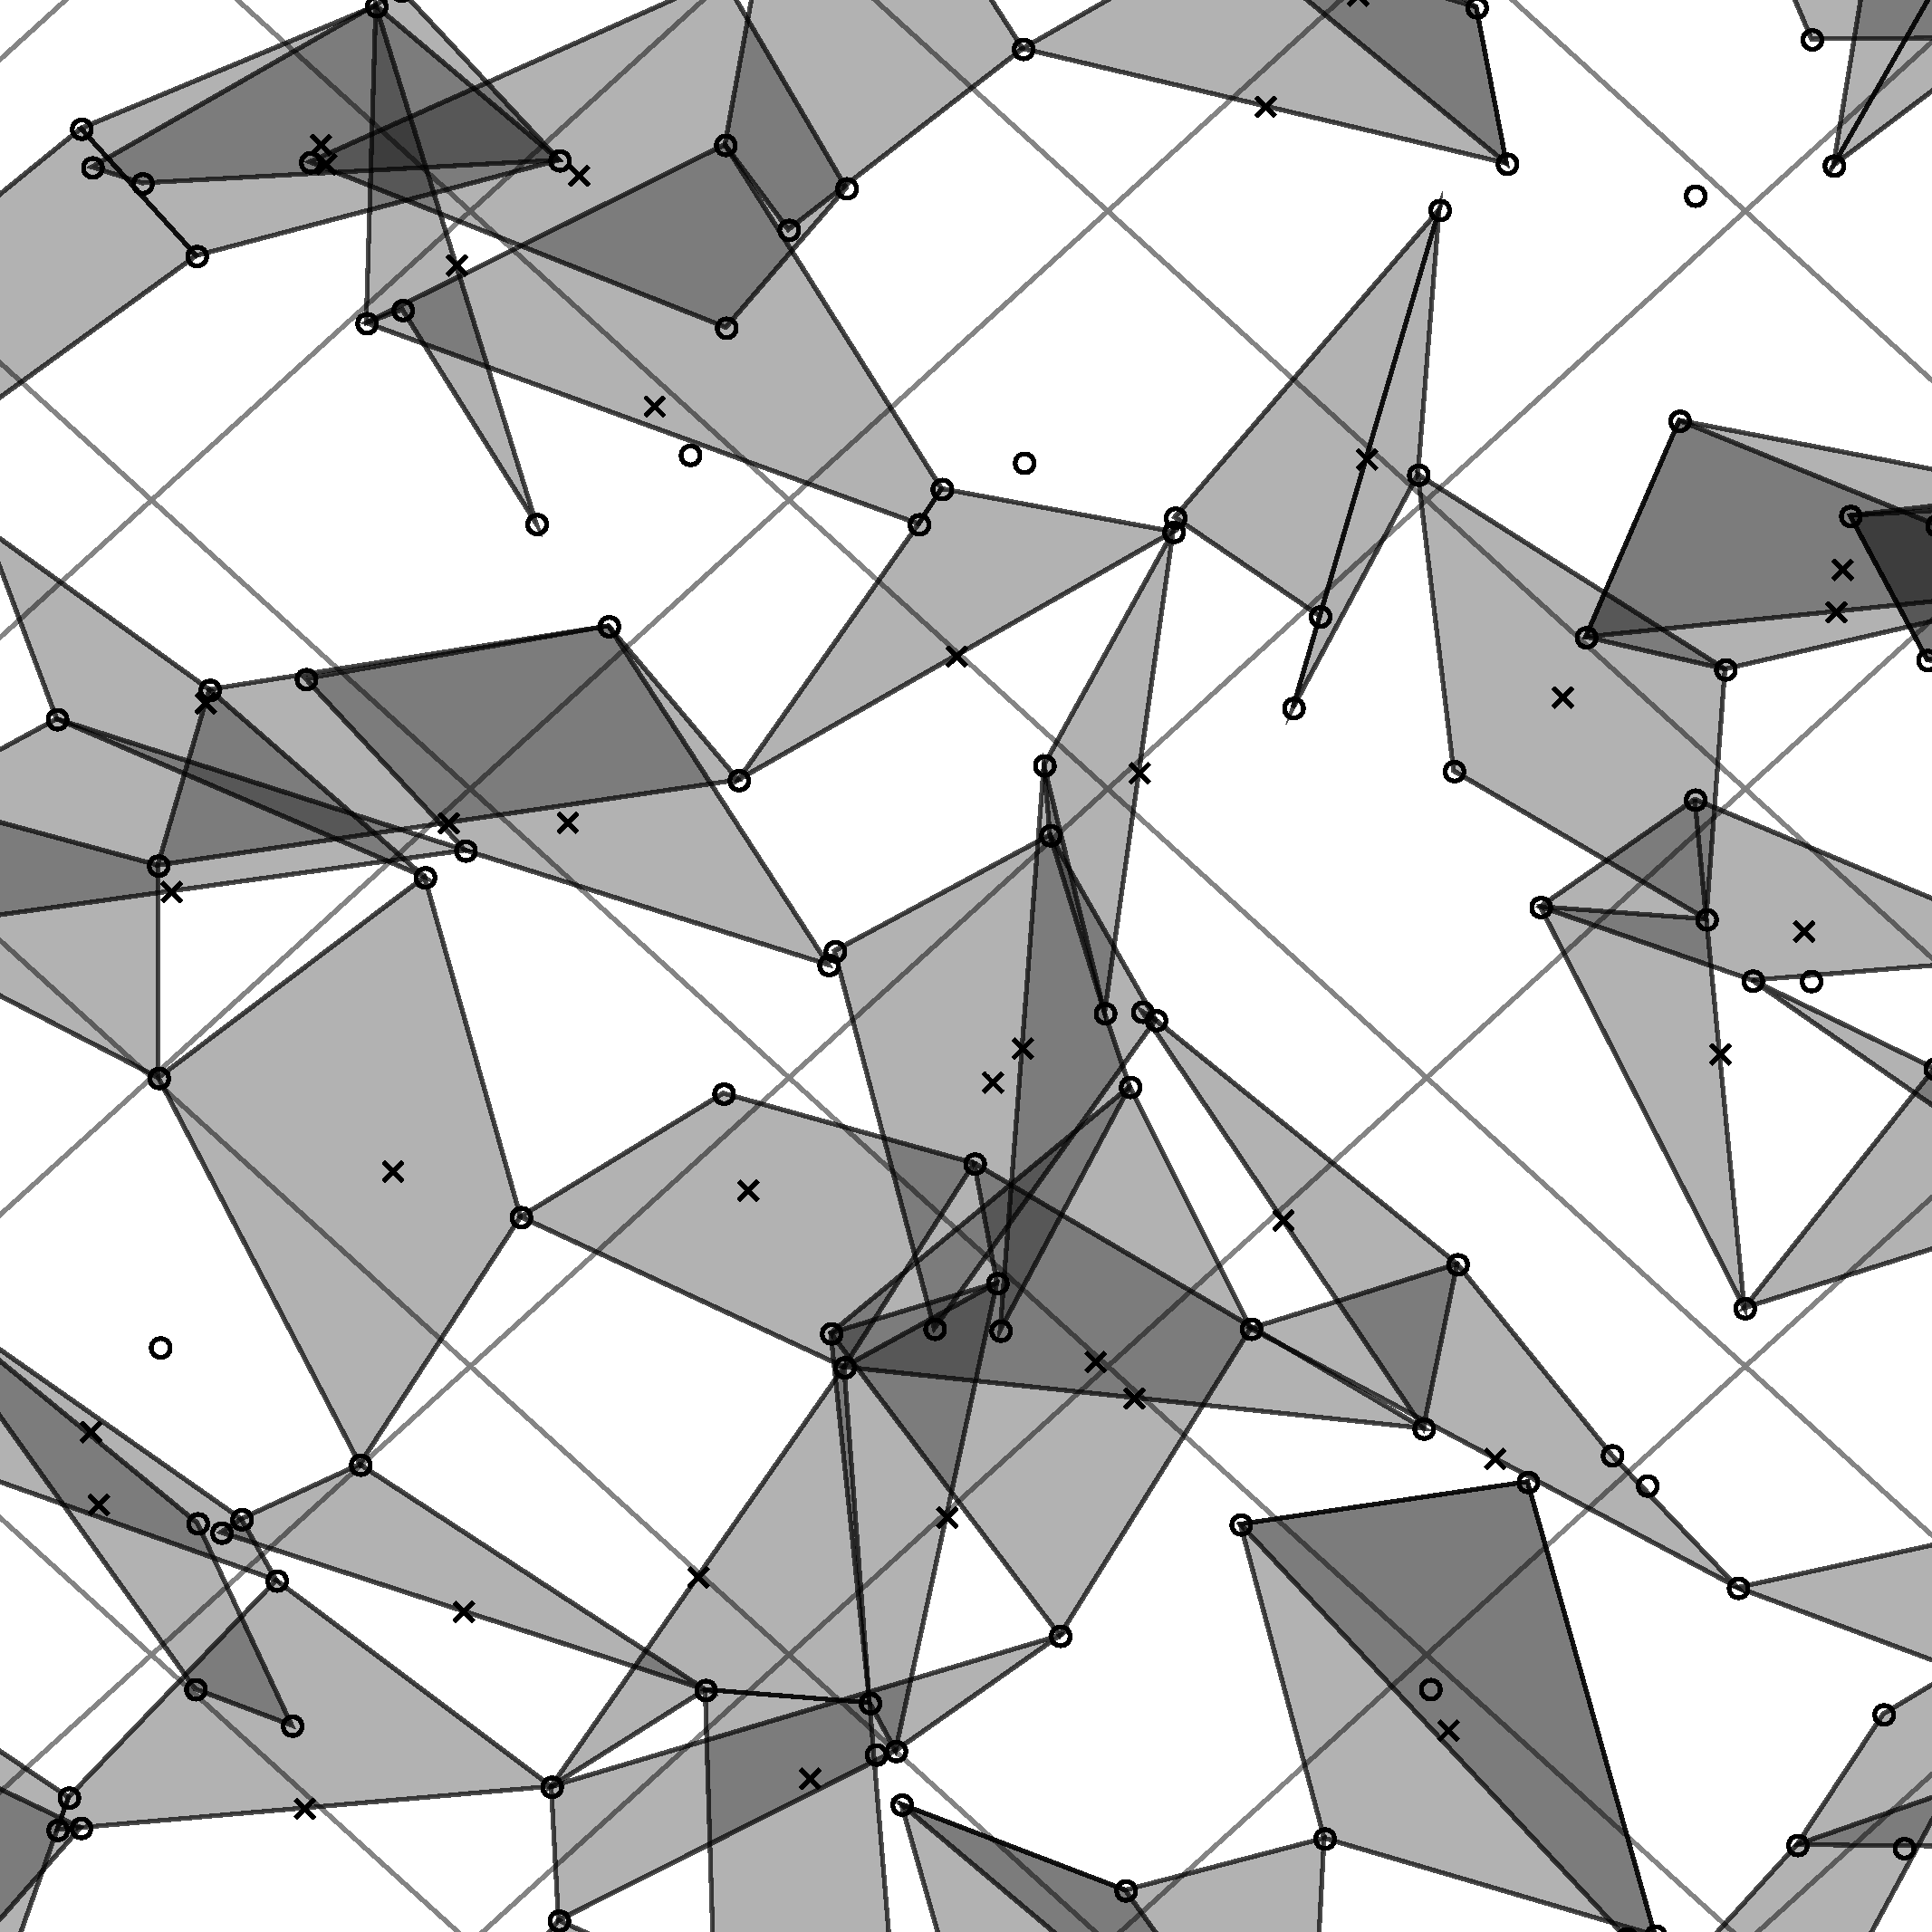
\includegraphics[width=0.99\textwidth]{quads2b}}
\end{center}
\caption{The same region of sky as in the previous figures, showing the
quads that are created after the second round of attempting to build a
quad in each grid cell.
\label{fig:quad2}}
\end{figure}


Next, we visit each grid cell and attempt to find a quad within the
acceptable range of angular sizes and whose center lies within the
grid cell.  We search for quads starting with the brightest stars, but
for each star we track the number of times it has already been used to
build a quad, and we skip stars that have been used too many times
already.  We repeat this process, sweeping through the grid cells and
attempting to build a quad in each one, a number of times.  In some
grid cells we will be unable to find an acceptable quad, so after this
process has finished we make further passes through the grid cells,
removing the restriction on the number of times a star can be used,
since it is better to have a quad comprised of over-used stars than no
quad at all.  Typically we make a total of $16$ passes over the grid
cells, and allow each star to be used in up to $8$ quads.  \Figs
\ref{fig:quad1} and \ref{fig:quad2} show the quads built during the first
two rounds of quad-building in our running example.


In principle, an index is simply a list of quads, where for each quad
we store its geometric hash code, and the identities of the four stars
of which it is composed (from which we can look up their positions on
the sky).  However, we want to be able to search quickly for all hash
codes near a given query hash code.  We therefore organize the hash
codes into a \kdtree data structure, which allows rapid retrieval of
all quads whose hash codes are in the neighborhood of any given query
hash code.  In order to carry out the verification step we also keep
the star positions in a \kdtree, since for each matched quad we need
to find other stars that should appear in the image if the match is
true.  Since none of the available \kdtree implementations were
satisfactory for our purposes, we created a fast, memory-efficient,
pointer-free \kdtree
\thesisonly{implementation.}
\notthesisonly{implementation \cite{dstnthesis}.}
%
\thesisonly{Our \kdtree implementation is presented in detail
in \chapref{chap:kdtree}.}


\begin{figure}[htp]
\begin{center}
\setlength{\fboxsep}{0.5pt}
\framebox{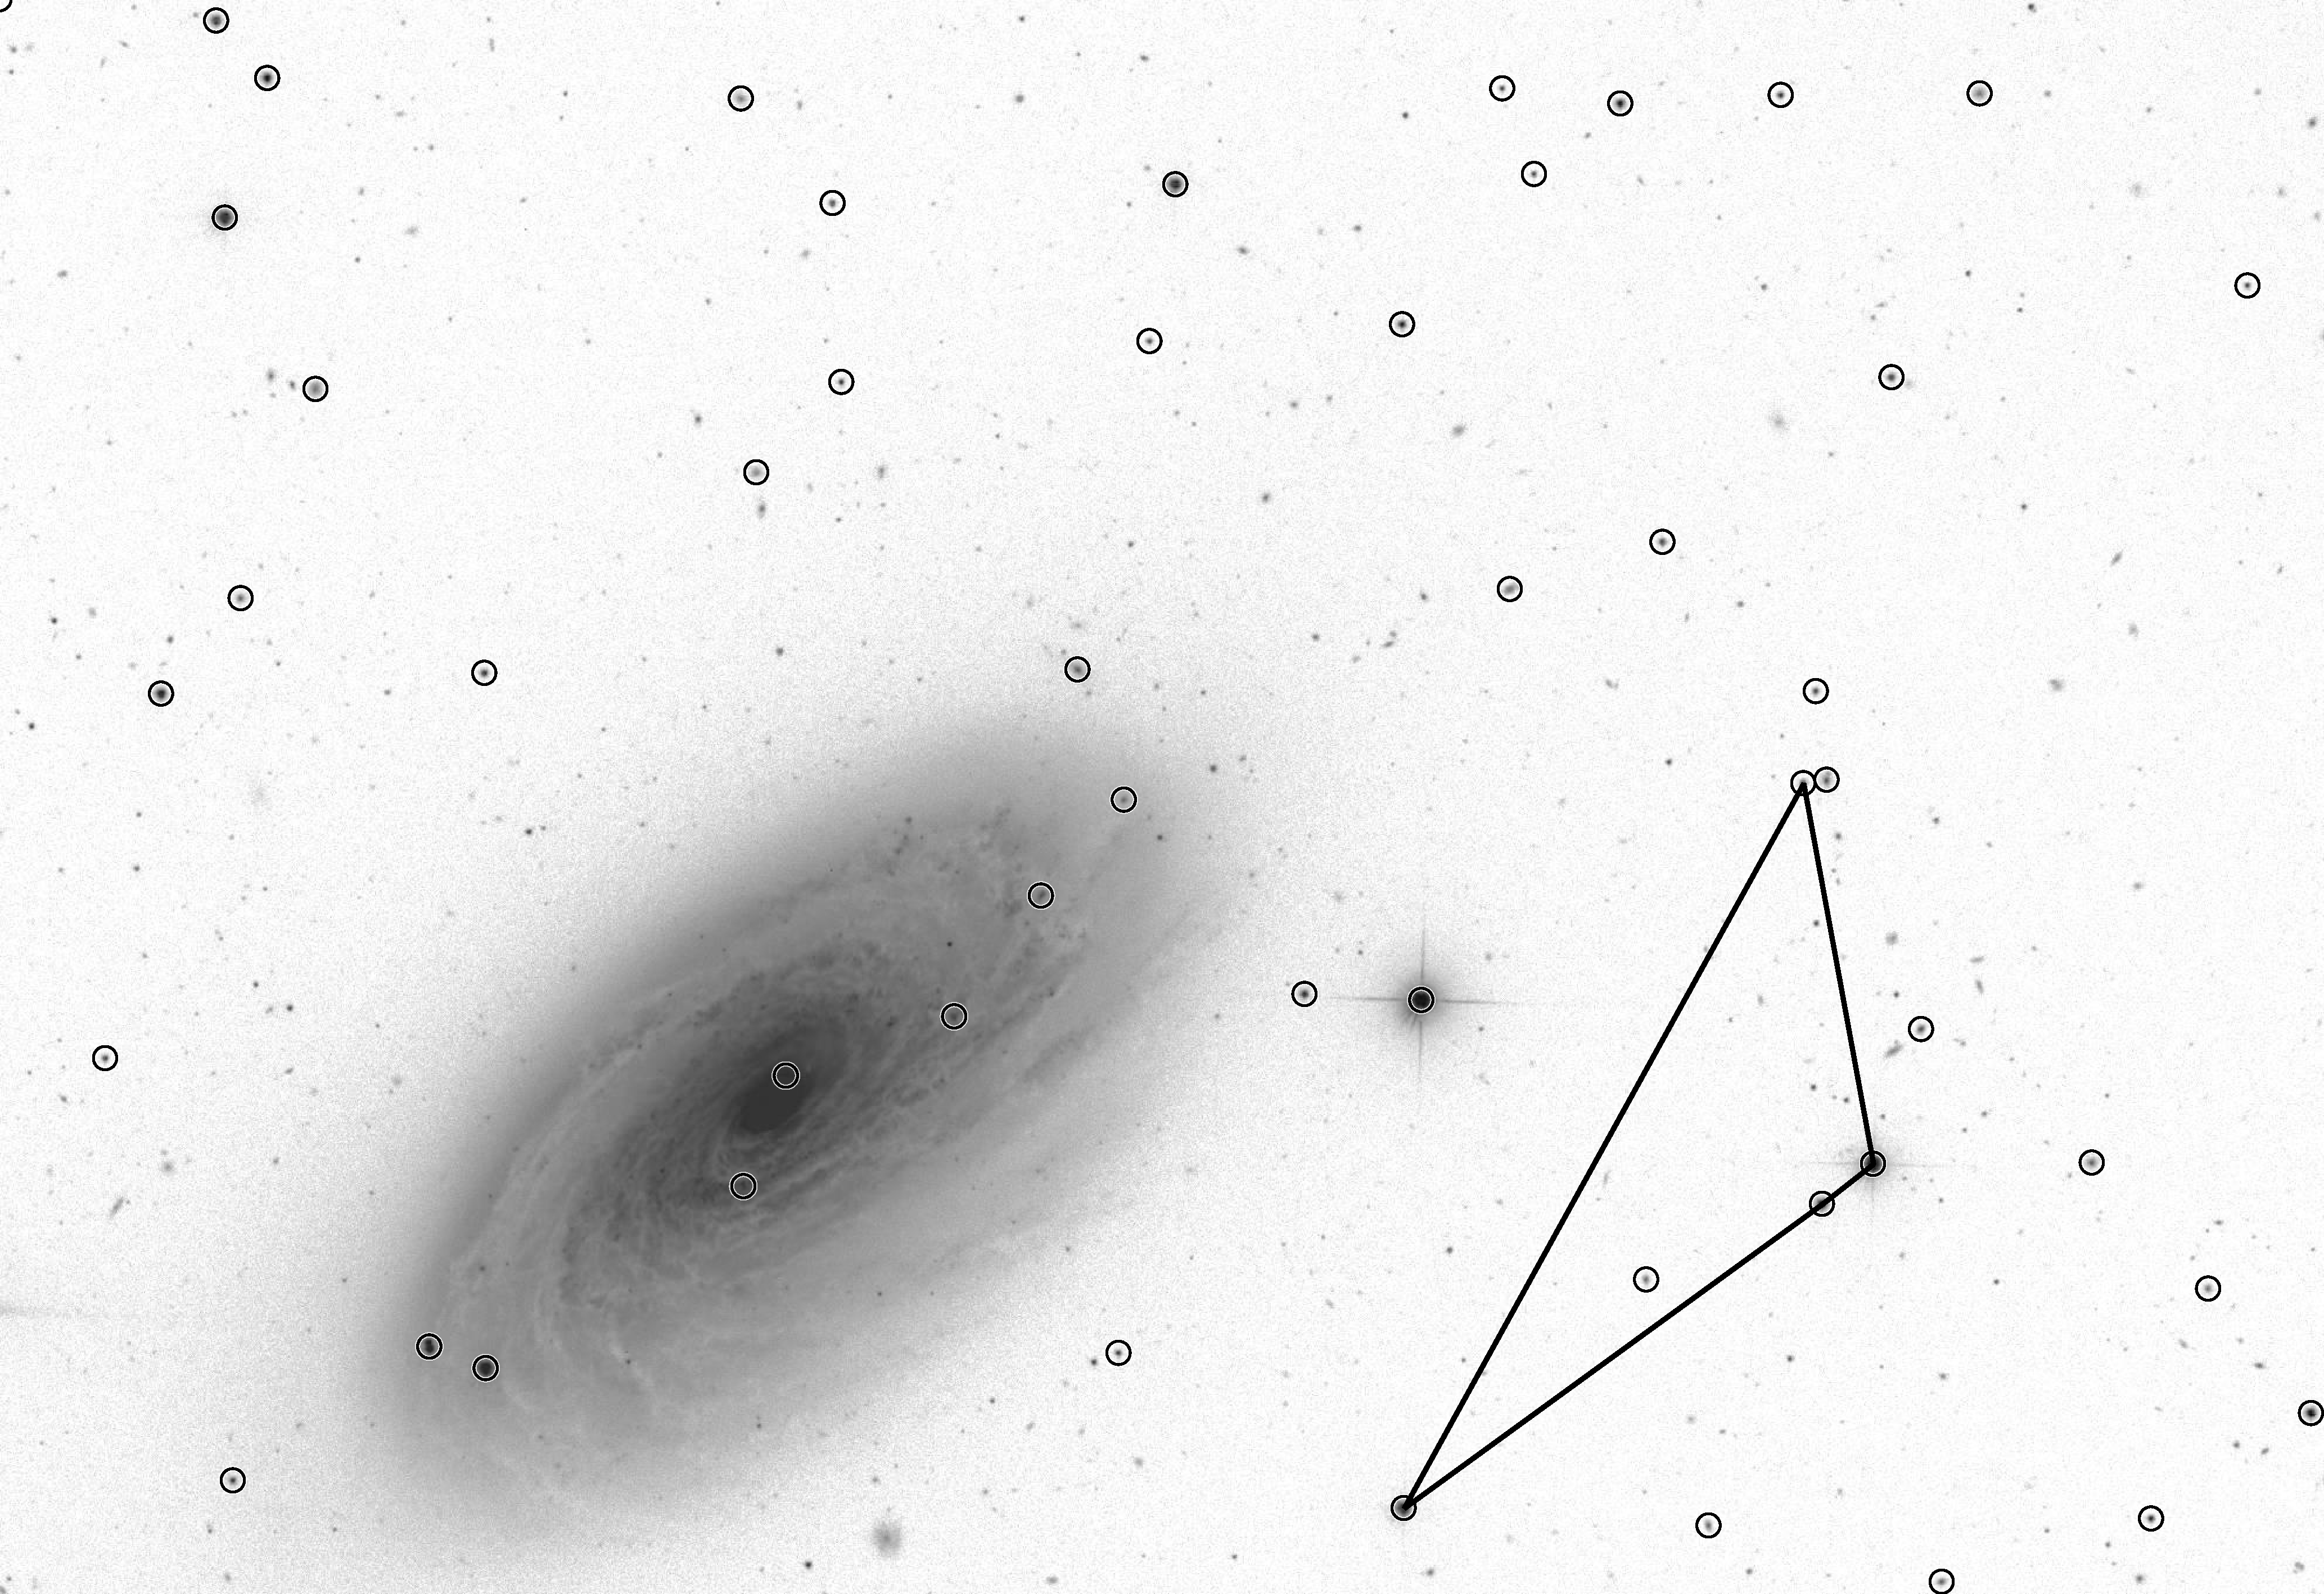
\includegraphics[width=0.99\textwidth]{m88-quad}}
\end{center}
\caption{A sample query image, with the brightest
$100$ sources our system detects (circles), and a quad in the image to
which our system will search for matches in the index.  This quad
looks like a triangle because two of its stars are nearly collinear.
Image credit: Sloan Digital Sky Survey.
\label{fig:imagequad}}
\end{figure}


\begin{figure}[htp]
\begin{center}
\setlength{\fboxsep}{0.5pt}
\framebox{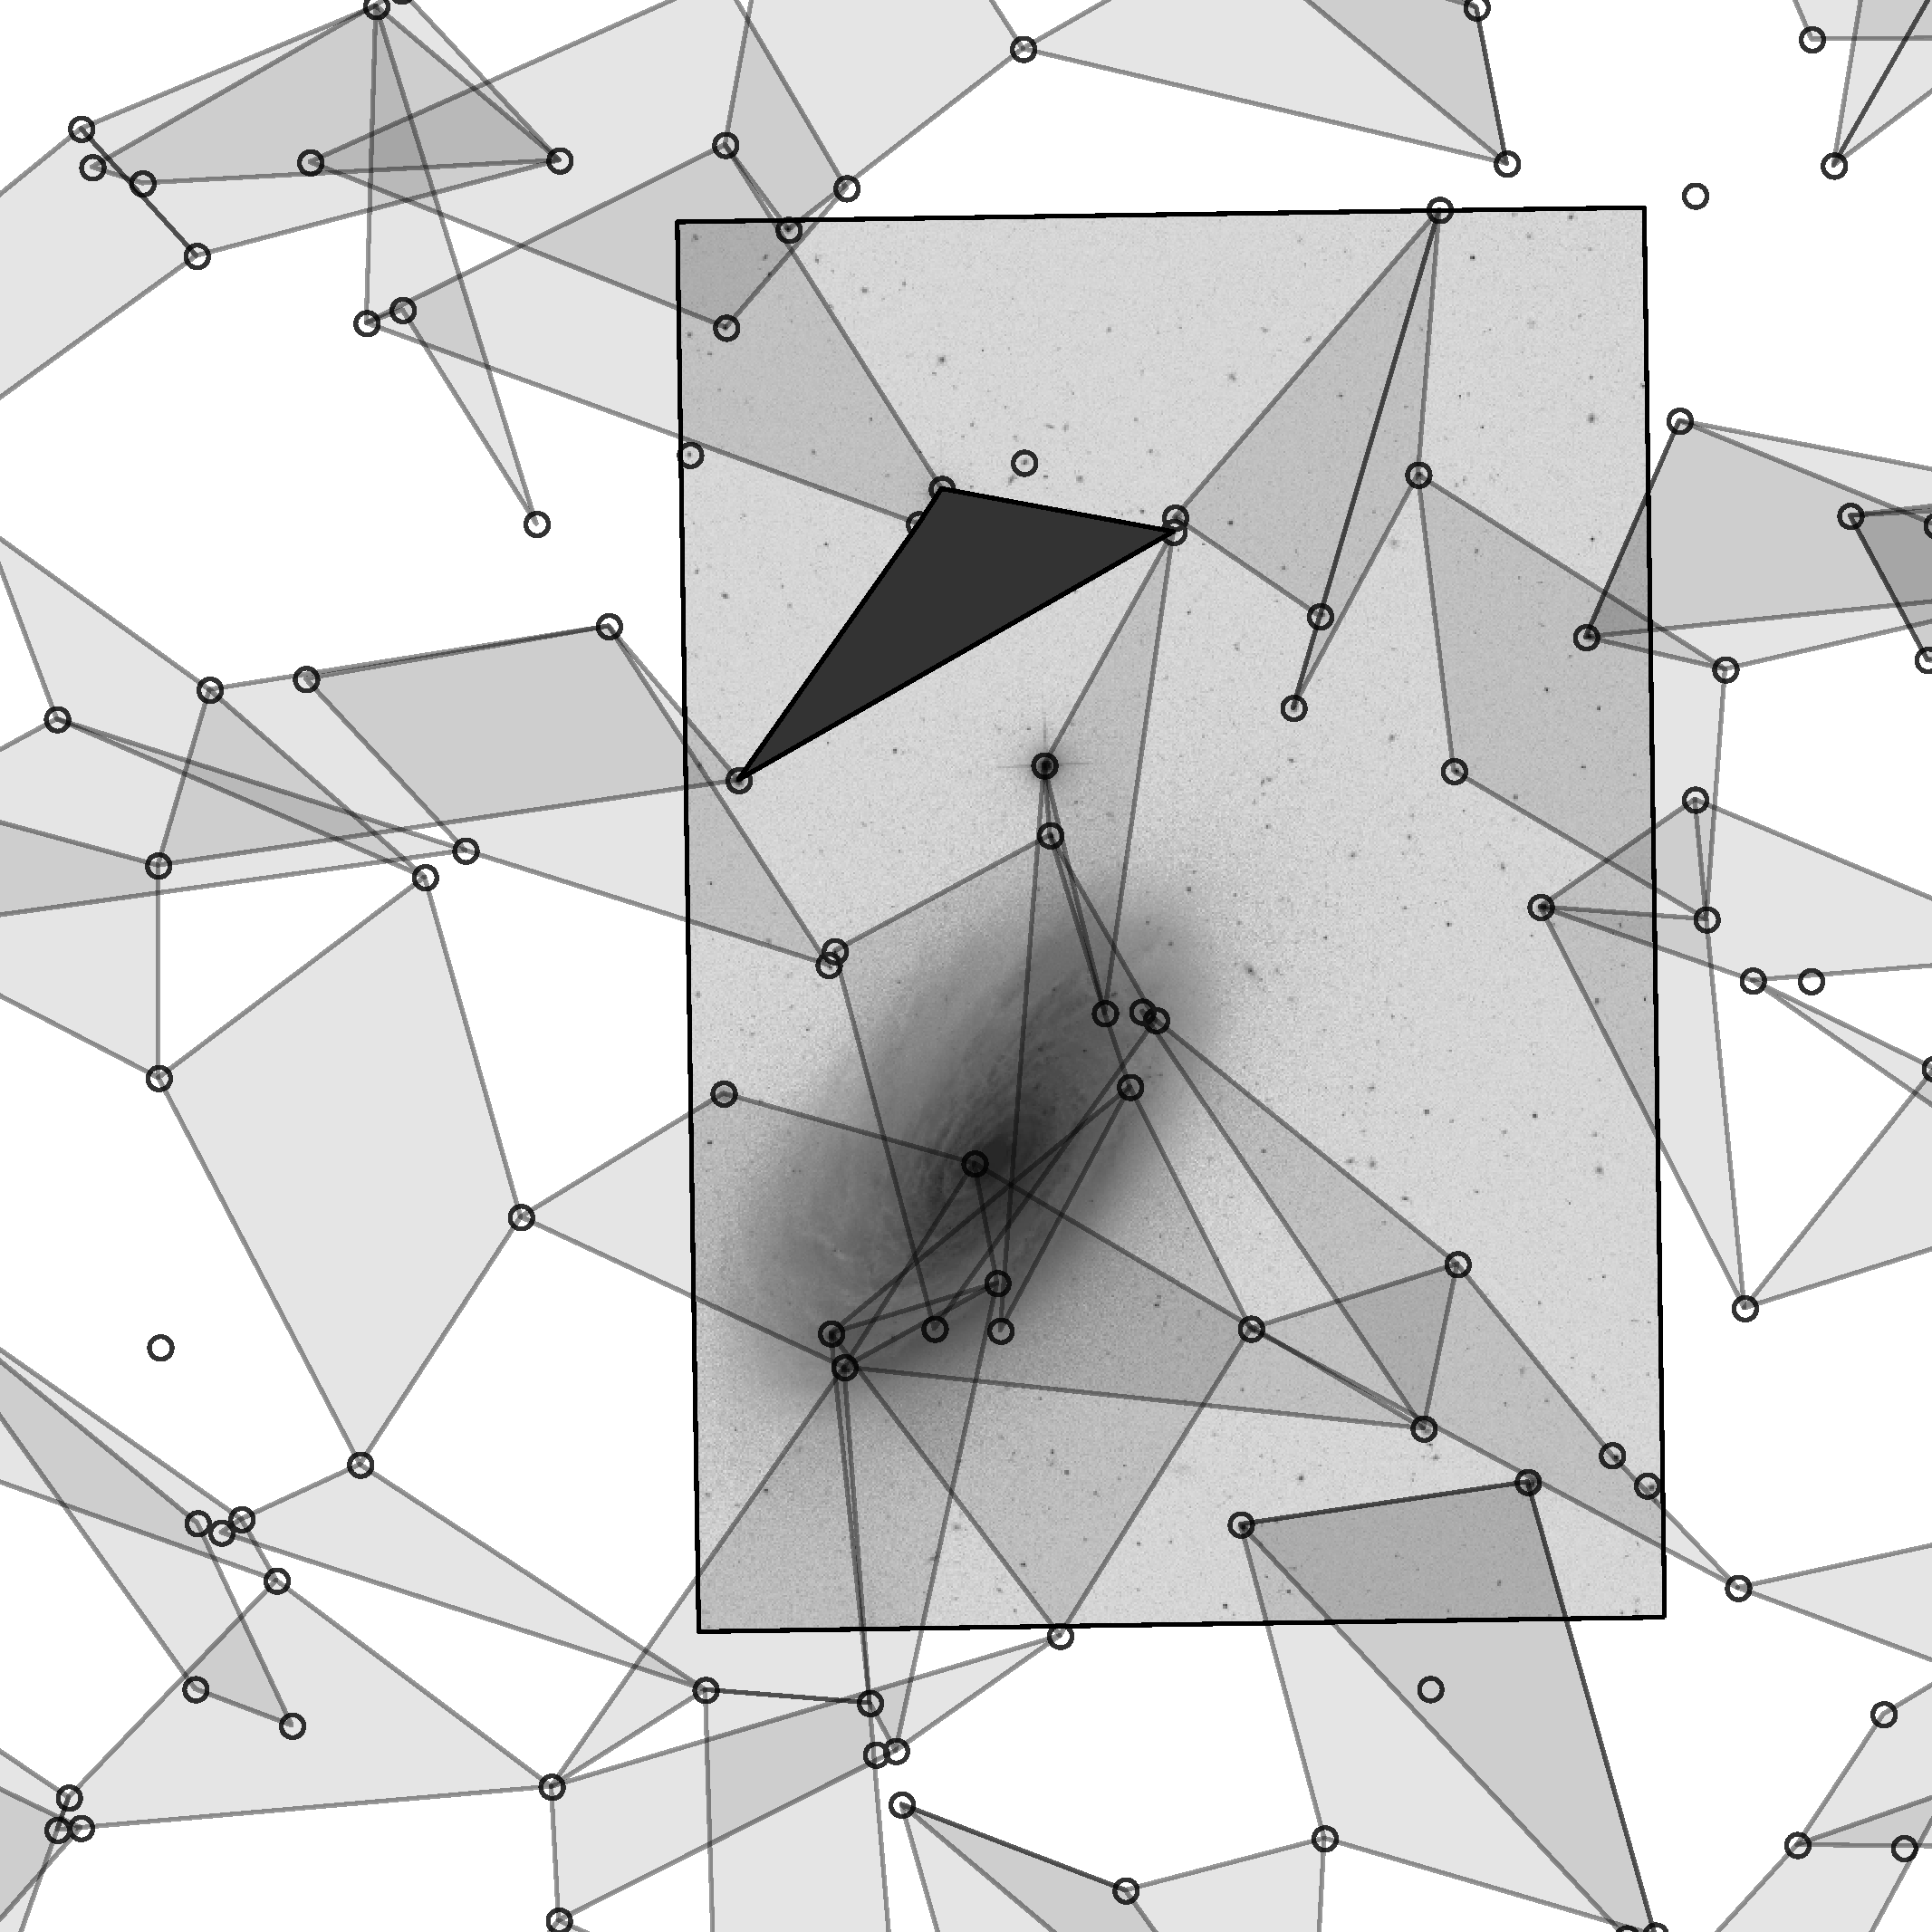
\includegraphics[width=0.99\textwidth]{match}}
%\includegraphics[width=\textwidth]{match}
\end{center}
\caption{Our example index, showing a quad in the index that matches 
a quad from the query image (shaded solid).  The image is shown
projected in its correct orientation on the sky.
\label{fig:quadmatch}}
\end{figure}


Given a query image, we detect stars as discussed above, and sort the
stars by brightness.  Next, we begin looking at quads of stars in the
image.  For each quad, we compute its geometric hash code and search
for nearby codes in the index.  For each matching code, we retrieve
the positions of the stars that compose the quad in the index, and
compute the hypothesized alignment---the World Coordinate System---of
the match.  We then retrieve other stars in the index that are within
the bounds of the image, and run the verification procedure to
determine whether the match is true or false.  We stop searching when
we find a true match in which we are sufficiently confident, or we
exhaust all the possible quads in the query image, or we run out of
time.  See \figref{fig:imagequad}.




\subsection{Verification of hypotheses}


The indexing system generates a large number of hypothesized
alignments of the image on the sky.  The task of the verification
procedure is to reject the large number of false matches that are
generated, and accept true matches when they are found.  Essentially,
we ask, ``if this proposed alignment were correct, where else in the
image would we expect to find stars?'' and if the alignment has very
good predictive power, we accept it.


We have framed the verification procedure as a Bayesian decision
process.  The system can either accept a hypothesized match---in which
case the hypothesized alignment is returned to the user---or the
system can reject the hypothesis, in which case the indexing system
continues searching for matches and generating more hypotheses.  In
effect, for each hypothesis we are choosing between two models: a
``foreground'' model, in which the alignment is true, and a
``background'' model, in which the alignment is false.  In Bayesian
decision-making, three factors contribute to this decision: the
relative abilities of the models to explain the observations, the
relative proportions of true and false alignments we expect to see,
and the relative costs or \emph{utilities} of the outcomes resulting
from our decision.


The \emph{Bayes factor} is a quantitative assessment of the relative
abilities of the two models---the foreground model $\fg$ and the
background model $\bg$---to produce or explain the observations.  In
this case the observations, or data, $\data$, are the stars observed
in the query image.  The Bayes factor
\begin{equation}
K = \frac{p(\data \given \fg)}{p(\data \given \bg)}
%\label{eq:bayesf}
\end{equation}
is the ratio of the marginal likelihoods.  We must also include in our
decision-making the prior $p(\fg)/p(\bg)$, which is our \emph{a
priori} belief, expressed as a ratio of probabilities, that a proposed
alignment is correct.  Since we typically examine many more false
alignments than true alignments (because we stop after the first true
alignment is found), this ratio will be small.
%
\notthesisonly{We typically set it, conservatively, to $10^{-6}$.}


The final component of Bayesian decision theory is the \emph{utility}
table, which expresses the subjective value of each outcome.  It is
good to accept correctly a true match or reject correctly a false
match (``true positive'' and ``true negative'' outcomes,
respectively), and it is bad to reject a true match or accept a false
match (``false negative'' and ``false positive'' outcomes,
respectively).  In the \an setting, we feel it is very bad to produce
a false positive: we would much rather fail to produce a result rather
than produce a false result, because we want the system to be be able
to run on large data sets without human intervention, and we want to
be confident in the results.
%
\notthesisonly{%
Our utility table is shown here.
\begin{center}
  \newcommand{\spacer}{\hspace{0.7em}}
\centering
\begin{tabular}{|c|c|r@{$\ $}l|r@{$\ $}l|}
  \cline{3-6}
    \multicolumn{2}{c|}{} & \multicolumn{4}{c|}{Reality \tstrut} \\
  \cline{3-6}
  \multicolumn{2}{c|}{} & \multicolumn{2}{c|}{True Alignment} & \multicolumn{2}{c|}{False Alignment \tstrut} \\
  \hline
  \multirow{2}{*}{Decision} &
  Accept & \spacer $u(\truepos) =$ & $+1$ & \spacer $u(\falsepos) =$ & $-1999$ \tstrut \\
  \cline{2-6}
  &
  Reject & $u(\falseneg) =$ & $-1$ & $u(\trueneg) =$ & $+1$ \tstrut \\
  \hline
\end{tabular}
\end{center}
}

\notthesisonly{%
Applying Bayesian decision theory, we make our decision to accept or
reject the hypothesized alignment by computing the expected utility
$\expect{u}$ of each decision.  The expected utility of accepting the
alignment is:
\begin{align}
\expect{u \given \mathrm{Accept}, \data}
&= u(\truepos) \, p(\truepos \given \data) + u(\falsepos) \, p(\falsepos \given \data) \\
&= u(\truepos) \, p(\fg \given \data) + u(\falsepos) \, p(\bg \given \data)
\end{align}
while the expected utility of rejecting the alignment is:
\begin{align}
\expect{u \given \mathrm{Reject}, \data}
&= u(\falseneg) \, p(\falseneg \given \data) + u(\trueneg) \, p(\trueneg \given \data) \\
&= u(\falseneg) \, p(\fg \given \data) + u(\trueneg) \, p(\bg \given \data) \quad .
\end{align}
We should accept the hypothesized alignment if:
\begin{align}
\expect{u \given \mathrm{Accept}, \data} 
&>
\expect{u \given \mathrm{Reject}, \data} \\
%
u(\truepos) \, p(\fg \given \data) + u(\falsepos) \, p(\bg \given \data)
&>
u(\falseneg) \, p(\fg \given \data) + u(\trueneg) \, p(\bg \given \data) \\
\frac{p(\fg \given \data)}{p(\bg \given \data)}
&>
\frac{u(\trueneg) - u(\falsepos)}{u(\truepos) - u(\falseneg)} \\
%
K &> \frac{p(\bg)}{p(\fg)} \ \frac{u(\trueneg) - u(\falsepos)}{u(\truepos) - u(\falseneg)}
\label{eq:kthresh}
\end{align}
where we have applied Bayes' theorem to get
\begin{equation}
\frac{p(\fg \given \data)}{p(\bg \given \data)} = K \ \frac{p(\fg)}{p(\bg)} \quad .
\end{equation}
}

\notthesisonly{%
With the prior and utilities given above, we find that we should
accept a hypothesis if:
\begin{align}
K &> \frac{p(\bg)}{p(\fg)} \ \frac{u(\trueneg) - u(\falsepos)}{u(\truepos) - u(\falseneg)} \\
K &> 10^6 \ \frac{1 - -1999}{1 - -1} \\
K &> 10^9
\end{align}
}


\notthesisonly{
That is, we accept a proposed alignment if the Bayes factor of the
foreground model to the background model exceeds a threshold that is
set based on our desired operating characteristics.  In our case, the
threshold is large so the foreground model (in which the alignment is
true) must be far better at explaining (\ie, predicting) the observed
positions of stars in the query image than the background model (in
which the alignment is false).}

\thesisonly{
Applying Bayesian decision theory given our desired operating
characteristics, we find that we should accept a proposed alignment
only if the Bayes factor is exceedingly large.  That is, the
foreground model in which the alignment is true must be far better at
explaining the observed positions of stars in the query image than the
background model that the alignment is false.  We typically set the
Bayes factor threshold to $10^9$ or $10^{12}$, but as will be shown in
the experiments below, we could set it even higher.  This threshold is
computed from our (subjective) desired operating characteristics, so
is not derivable from first principles.
}

In the foreground model, $\fg$, the four stars in the query image and
the four stars in the index are aligned.  We therefore expect that
other stars in the query image will be close to other stars in the
index.  However, we also know that some fraction of the stars in the
query image will have no counterpart in the index, due to occlusions
or artifacts in the images, errors in star detection or localization,
differences in the spectral bandpass, or because the query image
``star'' is actually a planet, satellite, comet, or some other
non-star, non-galaxy object.  True stars can be lost, and false stars
can be added.  Our foreground model is therefore a mixture of a
uniform probability that a star will be found anywhere in the
image---a query star that has no counterpart in the index---plus a
blob of probability around each star in the index, where the size of
the blob is determined by the combined positional variances of the
index and query stars.


Under the background model, $\bg$, the proposed alignment is false, so
the query image is from some unknown part of the sky; the index is not
useful for predicting the positions of stars in the image.  Our simple
model therefore places uniform probability of finding stars anywhere
in the test image.  \notthesisonly{We have experimented with a more
sophisticated background models that adapts to the observed
distribution of image stars, but we do not discuss that work here.}


The verification procedure evaluates stars in the query image, in
order of brightness, under the foreground and background models.  The
product of the foreground-to-background ratios is the Bayes factor.
We continue adding query stars until the Bayes factor exceeds our
threshold for accepting the match, or we run out of query stars.


\thesisonly{There are some subtleties in the verification process
which are explored in depth in \chapref{chap:verify}.}


\section{Results}

\subsection{Blind astrometric calibration of the Sloan Digital Sky Survey}

We explored the potential for automatically organizing and annotating
a large real-world data set by taking a sample of images generated by
the Sloan Digital Sky Survey and considering them as an unstructured
set of independent queries to our system.  For each SDSS image, we
discarded all \metadata, including all positional and rotational
information and the date on which the exposure was taken.  We allowed
ourselves to look only at the two-dimensional positions of detected
``stars'' (most of which were in fact stars but some of which were
galaxies or detection errors) in the image.  Normally, our system
would take \emph{images} as input, running a series of image
processing steps to detect stars and localize their positions.  The
SDSS data reduction pipeline already includes such a process, so for
these experiments we used these detected star positions rather than
processing all the raw images ourselves.  Further experiments have
shown that we would likely have achieved similar, if not better,
results by using our own image processing software.


\begin{figure}[htp]
\begin{center}
%\sdssquadfig
\includegraphics[width=\figunit]{sdss-quad-bw}
\end{center}
%\caption{A typical SDSS image, with the \iband-, \rband-, and
%\gband-band exposures mapped to the red, green, and blue channels of the image.
%The range of quad diameters that we use in the experiments below is
%shown by the circles.
\caption{A typical image from the Sloan Digital Sky Survey (SDSS).
The range of quad diameters that we use in the experiments below is
shown by the circles.  Image credit: Sloan Digital Sky Survey.
\label{fig:sdss}}
\end{figure}


Each SDSS image has $2048\times1489$ pixels and covers
$9\times13~\arcmin^2$, slightly less than one-millionth the area of
the sky.  Each image measures one of five bandpasses, called \uband,
\gband, \rband, \iband, and \zband, spanning the near-infrared through
optical to near-ultraviolet range.  Each band receives a $54$-second
exposure on a $2.5$-meter telescope.  A typical image is shown in
\figref{fig:sdss}.


The SDSS image-processing pipeline assigns to each image a quality
rating: ``excellent'', ``good'', ``acceptable'', or ``bad''.  We
retrieved the source positions (\ie, the list of objects detected by
the SDSS image-processing pipeline) in every image within the main
survey (Legacy and SEGUE footprints), using the public Catalog Archive
Server (CAS) interface to Data Release 7 \cite{sdssdr7}.  We retrieved
only sources categorized as ``primary'' or ``secondary'' detections of
stars and galaxies, and required that each image contained at least
$300$ objects.  The images that are excluded by these cuts contain
either very bright stars or peculiarities that cause the SDSS
image-processing pipeline to balk.  The number of images in Data
Release 7 and our cut is given in the table below.

%% FIXME --- histogram figure showing the 300 cut is reasonable.

%% 427,343 - distinct run,field,camcol in Field (fieldrfc)
%% 426,440 - distinct run,field,camcol in PhotoObjAll (allrfc)
%%    (903) - mostly bright stars; non-photometric
%% 421,381 - goodfields
%%  (5,059) - mostly mode=3, some mode=5, one mode=2
%%            --> quality	count
%%            --> 0	        3668   (bad)
%%            --> 1	        319    (acc)
%%            --> 2	        481    (good)
%%            --> 3	        591    (exc)
%%  see http://trac.astrometry.net/wiki/SdssCasNotes
%
% MyTable_3
%% 3	183359
%% 2	101490
%% 1	48802
%% 0	93692

\nonumberparagraphs
\begin{center}
\begin{tabular}{|l|D{,}{,}{3.3}|D{,}{,}{3.3}|}
\hline
\tableheaderx{Quality} & \tableheader{Total number of images} &
\tableheader{Number of images in our cut} \\
\hline
excellent & 183,359 & 182,221 \\
good & 101,490 & 100,763 \\
acceptable & 48,802 & 48,337 \\
bad & 93,692 & 89,219 \\
\hline
total & 427,343 & 420,540 \\
\hline
\end{tabular}
\end{center}
\numberparagraphs



\subsubsection{Performance on excellent images}


%%%%   The stats quoted in this section are using index 702.
%%%%      runs sdss-{1,11,12}
%%%%   I also ran 1302 and got almost exactly the same results.
%%%%      runs sdss-{16,17,18}


In order to show the best performance achievable with our system, we
built an index that is well-matched to SDSS \rband-band images.
Starting with the red bands from a cleaned version of the \USNOB, we
built an index containing stars drawn from a \healpix grid with cell
sizes about $4\times4~\arcmin^2$, and $10$ stars per cell.  We then
built quads with diameters of $4$ to $5.6~\arcmin$.  For each grid
cell, we searched for a quad whose center was within the grid cell,
starting with the brightest stars but allowing each star to be used at
most $8$ times.  We repeated this process $16$ times.  The index
contains a total of about $100$ million stars and $150$ million quads.
\Figref{fig:density} shows the spatial distribution of the stars and
quads in the index.

% index 702, cut 402: nside=880 -> ~4 arcmin.  4-5.6' quads.
% (for x in index-702-*.fits; do modhead $x NSTARS; done) | gawk 'BEGIN{N=0} {N+=$3} END{print N}'

\begin{figure}[htp]
% The three subfigures were made with:
%
% downsample-fits ~/go/AN/an-plotcat.fits /tmp/fifth.fits -v -s 5
% an-fitstopnm -i /tmp/fifth.fits -N 0 -X 300 -s | pnminvert | pnmtopng -transparent white > usnob-density.png
%
% (cd ~/go/CUTS/400; ./402-allsky.sh;
%   fitscopy cut-402-allsky.objs"[#row <  50000000]" cut-402-allsky-1.objs;
%   fitscopy cut-402-allsky.objs"[#row >= 50000000]" cut-402-allsky-2.objs;
%   modhead cut-402-allsky-1.objs NSTARS 49999999
%   modhead cut-402-allsky-2.objs NSTARS 42888778
%   plotcat -h -N 5000 -S -F -s -o 402-allsky-plotcat.fits cut-402-allsky-{1,2}.objs;
%   downsample-fits 402-allsky-plotcat.fits /tmp/fifth.fits -v -s 5;
%   an-fitstopnm -M -v -i /tmp/fifth.fits -N 0 -X 19.12 -s | pnminvert | pnmtopng -transparent white > cut-402-density.png
% )
%     # Median value: 9.56
%
% (cd ~/go/INDEXES/1300;
%  quadcenters -r 1302-quads0.rdls index-1302-0*
%  quadcenters -r 1302-quads1.rdls index-1302-1*
%  quadcenters -r 1302-quads2.rdls index-1302-2*
%  quadcenters -r 1302-quads3.rdls index-1302-3*
%  quadcenters -r 1302-quads4.rdls index-1302-4*
%  plotcat -h -N 5000 -S -F -s -o 1302-quads-plotcat.fits 1302-quads[01234].rdls;
%  downsample-fits 1302-quads-plotcat.fits /tmp/fifth.fits -v -s 5;
%  an-fitstopnm -M -v -i /tmp/fifth.fits -N 0 -X 30.56 -s | pnminvert | pnmtopng -transparent white > index-1302-density.png
%     # Median value: 15.28
% )
%
% Index 1300 is just like 700 but doesn't do the healpix grid-shifting thing
% (which leaves a very tiny bias in the quad positions that shows up in the plot)
%
% The subfigures are combined in the Latex document density-fig.tex
%
\begin{center}
% Only later versions of pdftex correctly handle png transparency, so make this a separate fig.
% ``oven'' builds it correctly.  ``monte'' does not.
\includegraphics[width=\textwidth]{density-fig}
\end{center}
\vspace{-20pt}
\caption{\captionpart{Top:} Density of sources in the \USNOB 
(in Hammer-Aitoff projection).
Dark colors indicate high density.  The north
    celestial pole is in the center of the image.  
	The dark strip through the center and
    around the edges is the Milky Way; lower-density dust lanes can be
    seen.
	% The two dense blobs at the right are the Large and Small
    % Magellanic Clouds.
	%
	The \USNOB was created by scanning
    photographic plates, and the places where the plates overlap are
    clearly visible as concentric rings and spokes of overdensities.
    \captionpart{Middle:} Density of sources in our spatially uniform
    cut of the \USNOB.  Most of the sky is
    very uniformly covered.  A few small bright (low-density) areas
    are visible, including a line near the bottom.  These are areas
    where the \USNOB is underdense due to defects.
    \captionpart{Bottom:} Density of quads in the index used in most
    of the experiments presented here.  Again, most of the sky is uniformly
	covered with quads.
\label{fig:density}}
\end{figure}


\begin{figure}[htp]
\begin{center}
    \sdssercputimefig
\end{center}
    \caption{Results from the excellent \rband-band SDSS images and
    \usnob-based index.  The percentage of images that are recognized
    correctly (\ie, astrometrically calibrated) with respect to the
    CPU time spent per image.  Many images are recognized rapidly, but
    there is a heavy tail of ``hard'' images.  Spending more and more
    CPU results in sharply diminishing returns.  After $1$ second,
    over $99.7~\percent$ of images are recognized, and after $10$
    seconds, over $99.97~\percent$ are recognized.  The steps are due
    to the finite resolution of the CPU timer we are using.
	\label{fig:sdsser1}}
\end{figure}

\begin{figure}[htp]
\begin{center}
\begin{tabular}{@{}c@{}c@{}}
\sdsserbayesfig & \sdsserntoverifyfig
\end{tabular}
\end{center}
\caption{Results from the excellent \rband-band SDSS images, continued.
	 \captionpart{Left:} The Bayes factor of the foreground model
    versus the background model for the hypotheses that we accept.
    The dashed line shows the threshold implied by our desired
    operating characteristics.  These excellent-quality images yield
    incredibly high Bayes factors---when we find a correct match is it
    unequivocal.  \captionpart{Right:} The number of stars in the
    query image that had to be examined before the Bayes-factor
    threshold was reached.  \label{fig:sdsser2}}
\end{figure}

\begin{figure}[htp]
\begin{center}
\begin{tabular}{@{}c@{}c@{}}
    \sdssercodeerrfig & \sdssernimagefig \\
\end{tabular}
\end{center}
    \caption{Results from the excellent \rband-band SDSS images,
    continued.  \captionpart{Left:} The distance in four-dimensional
    geometric hash code space between the query quad and the first
    correctly-matched index quad.  In this experiment we searched for
    matches within distance $0.01$: well into the tail of the
    distribution.  \captionpart{Right:} The number of stars in the
    query image that the system built quads from before finding the
    first correct match.  In a few cases, the brightest $4$ stars
    formed a valid quad which was matched correctly to the index: we
    got the correct answer after our first guess!
\label{fig:sdsser3}}
\end{figure}


\begin{figure}[htp]
\begin{center}
\sdsserradecfig
\end{center}
    \caption{Distribution of the excellent-quality \rband-band SDSS
    images on the sky.  The gray footprint represents the
    correctly-recognized images, while the black dots show the images
    that were not recognized using the \usnob-based index.  There is a
    slight overdensity of failures near the beginnings and ends of
    runs, but otherwise no apparent spatial structure.
\label{fig:sdsser4}}
\end{figure}


% Could plot: number of quads tried wrt number of stars examined.


We randomized the order of the excellent-quality \rband-band images,
discarded all astrometric \metadata---leaving only the pixel positions
of the brightest $300$ stars---and asked our system to recognize each
one.  We allowed the system to create quads from only the brightest
$50$ stars.  All $300$ stars were used during the hypothesis-checking
step, but since the Bayes factors tend to be overwhelmingly large, we
would have found similar results if we had kept only the $50$
brightest stars.  We also told our system the angular size of the
images to within about $1~\percent$, though we emphasize that this was
merely a means of reducing the computational burden of this
experiment: we would have achieved exactly the same results (after
more compute time) had we provided no information about the scale
whatsoever; we show this in \secref{sec:sizehints} below.


\nonumberparagraphs
\begin{center}
\sdssertable
\end{center}
\numberparagraphs


The results, shown in the table above and in \figs \ref{fig:sdsser1},
\ref{fig:sdsser2}, \ref{fig:sdsser3}, and \ref{fig:sdsser4}, are
that we can successfully recognize over $99.97~\percent$ of the
images.  We then examined our reference catalog, \usnob, at the true
locations of the images that were unrecognized.  Some of these
locations contained unusual artifacts.  For example,
\figref{fig:worms} shows a region where the
\usnob catalog contains ``worm'' features.  The cause of these
artifacts is unknown (David Monet, private communication), but they
affect several square degrees of one of the photographic plates that
were scanned to create the \usnob catalog.


\begin{figure}[htp]
\begin{center}
% python get_usnob.py -n "Worms" --fits 243 36
% an-fitstopnm -i usnob-243-36-*_se0275.000.fits -r -v | pnminvert | pnmtojpeg > worms.jpg
\includegraphics[width=0.5\textwidth]{worms}
\end{center}
\caption{``Worms'' in \usnob.  We found these unusual artifacts
by looking at one of the places where our system failed to recognize
SDSS images.  The image is of the photographic plate POSS-IE 275,
centered on $(\RA,\Dec) = (243, 36)~\degrees$ and $15\times15~\arcmin$
in size.  Image credit: Copyright Palomar Observatory, National
Geographic Society, and California Institute of Technology; courtesy
of USNO Image and Catalogue Archive.
\label{fig:worms}}
\end{figure}


In order to determine the extent to which our failure to recognize
images is due to problems with the \usnob reference catalog, we built
an index from the Two-Micron All-Sky Survey (2MASS) catalog, using the
same process as for the \usnob index, using the 2MASS
\band{J}-band rather than the \usnob red bands.  We then asked our
system to recognize each of the SDSS images that were unrecognized
using the \usnob-based index.  Of the $61$ images, $51$ were
recognized correctly, leaving only $10$ images unrecognized.
Examining these images, we found that some contained bright, saturated
stars which had been flagged as unreliable by the SDSS image-reduction
pipeline.  We retrieved the original data frames and asked our system
to recognize them.  All $10$ were recognized correctly: our source
extraction procedure was able to localize the bright stars correctly,
and with these the indexing system found a correct hypothesis.  With
these three processing steps, we achieve an overall performance of
$100~\percent$ correct recognition of all $182,221$ excellent images,
with no false positives.  This took a total of about $80$ minutes of
CPU time.  The index is about $5$ gigabytes in size, and once it is
loaded into memory, multiple CPU cores can use it in parallel, so the
wall-clock time can be a fraction of the total CPU time.  During this
experiment, a total of over $180$ million quads were tried, resulting
in about $77$ million matches to quads in the index.  Many of these
matches were found to result in image scales that were outside the
range we provided to the system, so the verification procedure was run
only $6$ million times.

% 702-slim: 4.7 GB.

% sdss-20

For completeness, we also checked the images that were rated as
excellent but failed our selection cut.  We retrieved the original
images and used our source extraction routine and both the \usnob- and
2MASS-based indexes.  Our system was able to recognize correctly all
$1138$ such images.


\subsubsection{Performance on images of varying bandpass}

% sdss-2

In order to investigate the performance of our system when the
bandpass of the query image is different than that of the index, we
asked the system to recognize images taken through the SDSS
filters \uband, \gband, \rband, \iband, and \zband.  We used only the
images rated ``excellent''.


\begin{figure}[htp]
\begin{center}
\begin{tabular}{@{}c@{}c@{}}
    \sdssbandsobjsfig & \sdssbandstimefig
\end{tabular}
\end{center}
\caption{Performance on images taken through different SDSS bandpass filters.
\captionpart{Left:} The percentage of images recognized after building quads
from a given number of the brightest stars in each image.  The
\rband-band is the best match to the \usnob-based index we are using.  Generally
the recognition rate drops with the distance between the bandpass of
the index and the bandpass of the image.  The \iband-band performance
in this instance is lower than expected.
\captionpart{Right:} The percentage of images recognized as the amount of
CPU time spent per image increases.  The \rband-band images are most
quickly recognized, \gband-, \iband-, and \zband-band images take
slightly more effort, and \uband-band images take considerably more
CPU time.  The asymptotic recognition rates are nearly identical
except for \uband-band, which is slightly lower.
\label{fig:sdssbands}}
\end{figure}

\nonumberparagraphs
\begin{center}
\sdssbandtable
\end{center}
\numberparagraphs

The results, shown in the table above and in \figref{fig:sdssbands},
demonstrate that as the difference between the query image bandpass
and the index bandpass increases, the amount of CPU time required to
recognize the same fraction of images increases.  This performance
drop is more pronounced on the blue (\uband) side than the red
(\zband) side.  After looking at the brightest $50$ stars, the system
is able to recognize essentially the same fraction of images.  As
shown by the first experiment in this section, this asymptotic
recognition rate is largely due to defects in the reference catalog
from which the index is built.


\subsubsection{Performance on images of varying quality}

% sdss-3

In order to characterize the performance of the system as image
quality degrades, we asked the system to recognize \rband-band images
that were classified as ``excellent'', ``good'', ``acceptable'', or
``bad'' by the SDSS image-reduction pipeline.

\nonumberparagraphs
\begin{center}
\sdssqualtable
\end{center}
\numberparagraphs

\begin{figure}[htp]
\begin{center}
\begin{tabular}{@{}c@{}c@{}}
    \sdssqualobjsfig & \sdssqualtimefig
\end{tabular}
\end{center}
\caption{Performance of the system given images of varying quality.
\captionpart{Left:} The percentage of images recognized after looking at a
given number of stars in each image, for excellent-, good-,
acceptable-, and bad-quality images from SDSS.  There is a small drop
in performance for good and acceptable images, and a more significant
drop for bad ones; all but the bad reach approximately the same
asymptotic recognition rate.  \captionpart{Right:} CPU time per image
for each quality rating.  All but the bad images show nearly
indistinguishable performance.
\label{fig:sdssqual}}
\end{figure}


The results, shown in the table above and in \figref{fig:sdssqual},
show almost no difference in performance between excellent, good, and
acceptable images.  Bad images show a significant drop in performance,
though we are still able to recognize over $99~\percent$ of them.


\subsubsection{Performance on images of varying angular size}

%%% FIXME - show image sizes with quad sizes superimposed.

% 13x9: sdss-1
% 9x9: sdss-4
% 8x8: sdss-5
% 7x7: sdss-8
% 6x6: sdss-9

\newcommand{\thirteenbynine}{\ensuremath{13\times9}}
\newcommand{\ninebynine}{\ensuremath{9\times9}}
\newcommand{\eightbyeight}{\ensuremath{8\times8}}
\newcommand{\sevenbyseven}{\ensuremath{7\times7}}
\newcommand{\sixbysix}{\ensuremath{6\times6}}
\newcommand{\arcminsquare}{\ensuremath{\textrm{arcmin}^2}}

We investigated the performance of our system with respect to the
angular size of the images by cropping out all but the central region
of the excellent-quality \rband-band images and running our system on
the sub-images.  Recall that the original image size is
$\thirteenbynine~\arcminsquare$, and that the index we are using
contains quads with diameters between $4$ and $5.6~\arcminsquare$.  We
cut the SDSS images down to sizes $\ninebynine$, $\eightbyeight$,
$\sevenbyseven$, and $\sixbysix~\arcminsquare$.  The $\sevenbyseven$
and $\sixbysix$ images required much more CPU time, so we ran only
small random subsamples of the images of these sizes.


\begin{figure}[htp]
\begin{center}
\begin{tabular}{@{}c@{}c@{}}
    \sdssimsizeobjsfig & \sdssimsizetimefig
\end{tabular}
\end{center}
\caption{Performance of the system given images of varying angular sizes.
\captionpart{Left:} The percentage of images recognized after looking at a
given number of stars in each image, for images of the given sizes.
Perhaps surprisingly, more of the $\eightbyeight$ images are
recognized correctly during the first few milliseconds, but as more
time elapses, the larger-scale images are more likely to be
recognized.
\captionpart{Right:}  CPU time per image required to recognize images of
each angular size.  After $10~\milliseconds$, the larger images are
recognized more quickly.  The $\sevenbyseven$ and $\sixbysix$ images
appear to be reaching asymptotic recognition rates far below
$100~\percent$.
\label{fig:sdssimsize}}
\end{figure}


\nonumberparagraphs
\begin{center}
\sdssimsizetable
\end{center}
\numberparagraphs


The results, presented in the table above and in
\figref{fig:sdssimsize}, show that performance degrades slowly for
images down to $\eightbyeight~\arcminsquare$, and then degrades
sharply.  This is not surprising given the size of quads in the index
used in this experiment: in the smaller images, only stars near the
edges of the image can possibly be $4$ to $5.6~\arcmin$ away from
another star, so the set of stars that can form the `backbone' of a
quad is small.  Observe that images below $2.8\times2.8~\arcminsquare$
cannot possibly be recognized by this index, since no pair of stars
can be $4~\arcmin$ or more away from each other.


This does not imply that small images cannot be recognized by our
system: given an index containing smaller quads, we may still be able
to recognize them.  The point is simply that for any given index there
is some threshold of angular size below which the image recognition
rate will drop, and another threshold below which the recognition rate
will be exactly zero.


\subsubsection{Performance with varying image scale hints}
\label{sec:sizehints}

% sdss-15

In all the experiments above, we told our system the angular scale (in
arcseconds per pixel) to within $\pm1.25~\percent$ of the true value,
and we used an index containing only quads within a small range of
diameters.  In this experiment, we show that these hints merely make
the recognition process faster without affecting the general results.


We created a set of sub-indices, each covering a range of $\sqrt{2}$
in quad diameters.  The smallest-scale sub-index contains quads of $2$
to $2.8~\arcmin$, and the largest contains quads of about $20$ to $30$
degrees in diameter.  Each sub-index is built using the same
methodology as outlined above for the $4$ to $5.6~\arcmin$ index, with
the scale adjusted appropriately.  The smallest-scale sub-index
contains only $6$ stars per \healpix grid cell rather than $10$ as in
the other sub-indices, because the \usnob catalog does not contain
enough stars: a large fraction of the smallest cells contain fewer
than $10$ stars.  In the smallest-scale sub-index we then do $9$
rounds of quad-building, reusing each star at most $5$ times, as
opposed to $16$ rounds reusing each star at most $8$ times as in the
rest of the sub-indices.


\begin{figure}[htp]
\begin{center}
%\begin{tabular}{@{}c@{}c@{}}
    \sdsssizehintsindexfig
%\end{tabular}
\end{center}
\caption{The sub-index that is first to recognize SDSS images, when all
the sub-indices are run in lock-step.  Although we used sub-indices
containing quads up to $30$ degrees in diameter, clearly only the ones
that contain quads that can possibly be found in an SDSS image (which
are about $16~\arcmin$ across the diagonal) can generate correct
hypotheses that will recognize the image.  Perhaps surprisingly, each
of these sub-indices is first to recognize some subset of the images,
though a strong tuning effect is clear.
\label{fig:sdsssizehintsindex}}
\end{figure}


Each time our system examines a quad in the image, it searches each
sub-index in turn for matching quads, and evaluates each hypothesized
alignment generated by this process.  The system proceeds in
lock-step, testing each quad in the image against each sub-index in
turn.  The first quad match that generates an acceptably good
alignment is taken as the result and the process stops.  Note that
several of the sub-indices may be able to recognize any given image.
Indeed, \figref{fig:sdsssizehintsindex} shows that every sub-index
that contains quads that can possibly be found in SDSS images is first
to recognize some of the images in this experiment.  Different
strategies for ordering the computation---for example, spending equal
amounts of CPU time in each sub-index rather than proceeding in
lock-step---might result in better overall performance.


\begin{figure}[htp]
\begin{center}
\begin{tabular}{@{}c@{}c@{}}
    \sdsssizehintstimefig & \sdsssizehintsreltimefig
\end{tabular}
\end{center}
\caption{Performance of the system given varying limits on the image size.
\captionpart{Left:} CPU time per image required to recognize images, given
various limits on the angular size of the image.  Our system achieves
the same asymptotic recognition rate in each case: giving the system
less information about the true scale of the image simply means that
it must evaluate and reject more false hypotheses before finding a
true one.  The ``$\ge8~\arcmin$'' hint indicates that we told the
system that the image width is between $8~\arcmin$ and $180~\degrees$.
The upper limit has much less impact on performance than the lower
limit, since the sub-indices that cover large angular scales contain
many fewer quads and are therefore much faster to search, and generate
fewer coincidental matches.  \captionpart{Right:} CPU time per image
relative to the $\pm1.25~\percent$ case.  We divided the CPU times for
each case into percentiles; the mean time within each percentile is
plotted.  Generally, giving the system less information about the size
of the images results in an approximately constant-factor increase in
the CPU time required.  Although there appears to be a sharp upward
trend for the ``loosest'' four size ranges, this may be an effect of
small sample size: since these cases take so long to run, we tested
only $1000$ images, while for the rest of the cases we tested $10,000$
images.  The CPU time distribution is heavy-tailed, so the expected
variance is large.
\label{fig:sdsssizehints}}
\end{figure}




\subsubsection{Performance with varying index quad density}

% sdss-1  (index 702)
% sdss-10 (index 1102, half as dense)
% sdss-13 (index 1202, quarter as dense)

The fiducial index we have been using in these experiments contains
about $16$ quads per \healpix grid cell.  Since each SDSS image has
an area of about $7$ cells, we expect each image to contain about
$100$ quad centers.  The number of complete quads (\ie, quads for
which all four stars are contained in the image) in the image will be
smaller, but we still expect each image to contain many quads.  This
gives us many chances of finding a correct match to a quad in the
image.  This redundancy comes at a cost: the total number of quads in
the index determines the rate of false matches---since the code-space
volume is fixed, packing more quads into the space results in a larger
number of matches to any given query point---which directly affects
the speed of each query.  By building indices with fewer quads, we can
reduce the redundancy but increase the speed of each query.  This does
not necessarily increase the overall speed, however: an index
containing fewer quads may require more quads from the image to be
checked before a correct match is found.  In this experiment, we vary
the quad density and measure the overall performance.


\nonumberparagraphs
\begin{center}
\sdssdensitytable
\end{center}
\numberparagraphs


\begin{figure}[htp]
\begin{center}
\begin{tabular}{@{}c@{}c@{}}
    \sdssdensitytimefig & \sdssdensityreltimefig
\end{tabular}
\end{center}
\caption{Performance of the system using indices containing varying
densities of quads.  (The total number of quads in an index is
proportional to the density of quads.)
\captionpart{Left:} CPU time per image required to recognize images.
\captionpart{Right:} Relative CPU time to recognize images.  We split
the set of images into percentiles and have plotted the mean time
within each percentile, relative to the 16-quad-per-cell reference
index.  The indices containing fewer quads are faster to search per
quad query, but may require more quads to be tried before a correct
match is found.  The smaller indices are also able to recognize fewer
images, because some images will simply not contain a quad that
appears in the index.  For the high-quality SDSS images we are using,
the smallest of the indices here results in a $2~\percent$ drop in
recognition rate (from nearly $100~\percent$ to about $98~\percent$),
but for poorer-quality images the drop could be larger.
\label{fig:sdssdensity}}
\end{figure}


As shown in the table above and \figref{fig:sdssdensity}, reducing the
density from $16$ to $9$ quads per \healpix grid cell has almost no
effect on the recognition rate but takes only two-thirds as much CPU
time.  Reducing the density further begins to have a significant
effect on the recognition rate, and actually takes \emph{more} CPU
time overall.


\subsubsection{Performance on indices built from triangles and quints}
\label{sec:triquint}

% sdss-32, 33, 34

% nquads
% ntries-brute
% time

We tested the performance of our quad-based index against a
triangle-based index and a quintuple-based (``quint'') index.  The
index-building processes were exactly as in our quad-based indices.

In the experiments above we searched for all matches within a distance
of $0.01$ in the quad feature space.  Since the triangle- and
quint-based indices have feature spaces of different dimensionalities
($2$ for triangles, $6$ for quints), we first ran our system with the
matching tolerance set to $0.02$ in order to measure the distribution
of distances of correct matches in the three feature spaces.  We then
set the matching tolerance to include $95~\percent$ of each
distribution.  For the triangle-based index, we found this matching
tolerance to be $0.0064$, for the quad-based index it was $0.0095$,
and for the quint-based index, $0.011$.  These experiments were
performed on a random subset of $4000$ images, because they are quite
time-consuming.

\nonumberparagraphs
\begin{center}
\sdsstriquinttable
\end{center}
\numberparagraphs


\begin{figure}[htp]
\begin{center}
\begin{tabular}{@{}c@{}c@{}}
\sdsstriquinttimefig & \sdsstriquintntrynmatchfig
\end{tabular}
\end{center}
\caption{Performance of the system using indices containing triangles,
quads, and quintuples of stars.  \captionpart{Left:} CPU time per
image required to recognize images.  The quad-based index vastly
outperforms the triangle- and quint-based indices.
\captionpart{Right:} The number of features tried (\ie, the number
of triangles, quads, or quints of stars from the image that were
tested), and the number of matches to features in the index that
resulted.  Each plotted point summarizes $2~\percent$ of the
correctly-recognized images, sorted by the number of features tried.
As expected, the triangle-based index produces many more matches for
any given query, because the same number of features are packed into a
lower-dimensional feature space.  Fewer features have to be tried
before the first correct matches are found, because only three
corresponding stars have to be found.  Quints, on the other hand, are
very distinctive: for over $80~\percent$ of the images that were
correctly recognized, the first matching quint ever found was a
correct match.  However, many quints from the image have to be tested
before this match is found.
\label{fig:sdsstriquint}}
\end{figure}


The results are given in the table above and in
\figref{fig:sdsstriquint}.  After looking at the brightest
$50$ stars in each image, the triangle-based index is able to
recognize the largest number of images, but both the triangle- and
quint-based indices take significantly more time than the quad-based
index.  It seems that quad features strike the right balance between
being distinctive enough that any given query does not generate too
many coincidental (false) matches---as the triangle-based index
does---but containing few enough stars that it does not take long to
find a feature that is in both the image and the index---as the
quint-based index does.


We expect that the relative performance of triangle-, quad-, and
quint-based indices depends strongly on the angular size of the images
to be recognized.  An index designed to recognize images of large angular
size requires fewer features, so the code space is less densely filled
and fewer false matches are generated.  For this reason, we expect
that above some angular size, a triangle-based index will recognize
images more quickly than a quad-based index.


%Perhaps surprisingly, the small decrease in the matching
%distance in feature space from $0.01$ to $0.0095$ for the quad-based
%index resulted in a $>0.6~\percent$ drop in recognition rate.


\subsection{Blind astrometric calibration of Galaxy Evolution Explorer data}

% GAL-4

To show the performance of our system on significantly larger images,
at a bandpass quite far from that of our index, we experimented with
data from the Galaxy Evolution Explorer (GALEX).  GALEX is a space
telescope that observes the sky through near- and far-ultraviolet
bandpass filters.  Although it is fundamentally a photon-counting
device, the GALEX processing pipeline renders images (by collapsing
the time dimension and histogramming the photon positions), and these
are the data products used by most researchers.  The images are
circular, with a diameter of about $1.2$ degrees.  See
\figref{fig:galexquad}.  In this experiment, rather than using the
images themselves, we use the catalogs (lists of sources found in each
image) that are released along with the images.  These catalogs are
produced by running a standard source extraction program (SExtractor)
on the images.  We retrieved the near-UV catalogs for all $28,182$
images in Galex Release 4/5 that have near-UV exposure.


\begin{figure}[htp]
\begin{center}
\galexquadfig
\end{center}
\caption{A sample GALEX field (AIS-101-sg32-nuv),
with circles showing the sizes of the quads in the indices we use in
this experiment.  The images produced by the GALEX pipeline are
$3840\times3840$ pixels, and the near-UV field of view is a circle of
diameter $1.24~\degrees$, or about $74.4~\arcmin$.  Image credit:
Courtesy NASA/JPL-Caltech.
\label{fig:galexquad}}

\end{figure}


% indices 705-709
% (for x in index-70[56789].fits; do modhead $x NSTARS; done) | gawk 'BEGIN{N=0} {N+=$3} END{print N}'
% 29,358,529
% (for x in index-70[56789].fits; do modhead $x NQUADS; done) | gawk 'BEGIN{N=0} {N+=$3} END{print N}'
% 36,146,408

We built a series of indices of various scales, each spanning roughly
$\sqrt{2}$ in scale.  The smallest contained quads with diameters from
$11$ to $16~\arcmin$, the next contained quads between $16$ and
$22~\arcmin$, followed by $22$ to $30$, $30$ to $42$, and $42$ to
$60~\arcmin$.  Each index was built according to the ``standard
recipe'' given above, using stars from the red bands of \usnob as
before.  In total these indices contain about $30$ million stars and
$36$ million quads.


\nonumberparagraphs
\begin{center}
\galextable
\end{center}
\numberparagraphs


In this experiment, we told our system that the images were between
$1$ and $2$ degrees wide, and we allowed it to build quads from the
first $100$ sources in each image.  The results are shown in the table
above and \figref{fig:galex}.  The recognition rate is quite similar
to that of the excellent-quality SDSS \rband-band fields, suggesting
that even though the near-UV bandpass of these images is quite far
from the bandpass of the index, which we would expect to make the
system less successful at recognizing these images, their larger
angular size seems to compensate.  The system is significantly slower
at recognizing GALEX images, but this is partly because we gave it a
fairly wide range of angular scales, and because we used several
indices rather than the single one whose scale is best tuned to these
images.


\begin{figure}[htp]
\begin{center}
\begin{tabular}{@{}c@{}c@{}}
    \galexcputimefig & \galexindexidfig
\end{tabular}
\end{center}
\caption{Results on GALEX near-UV images.  \captionpart{Left:} CPU
time used per image.  The shape of the curve is very similar to that
in the previous SDSS experiments, though the ``knee'' of diminishing
returns occurs after more CPU time (possibly because we gave the
system much less information about the correct scale of the images).
\captionpart{Right:} The number of images recognized by each of the
indices (identified by the range of sizes of quads they contain).  For
each quad in the image, we search for matches in each of the indices,
stopping after the first match that is confirmed by the verification
test.  The histogram therefore shows only which index recognized the
image \emph{first}, rather than which indices might have recognized it
given more time.  The inset histograms show the distribution of quad
sizes within each index (on a linear scale).  Generally the larger
quads are more successful, except in the largest index, where the size
of the largest quads approaches that of the whole image.
\label{fig:galex}}
\end{figure}


% Plot GALEX NUV along with SDSS ugriz.


\subsection{Blind astrometric calibration of Hubble Space Telescope data}


In order to demonstrate that there is nothing intrinsic in our method
that limits us to images of a particular scale, we retrieved a set of
Hubble Space Telescope (HST) images and built a custom index to
recognize them.  We chose the All-wavelength Extended Groth strip
International Survey (AEGIS) \cite{aegis} footprint because it has
many HST exposures and is within the SDSS footprint.


\begin{figure}[htp]
\begin{center}
\aegisacsquadsizesfig
\end{center}
\caption{The diameters of quads in our custom index, built from SDSS
stars, for recognizing Hubble Space Telescope Advanced Camera for
Surveys (ACS) images in the AEGIS footprint.  Although we allowed
quads with diameters between $0.5$ and $2~\arcmin$, the size
distribution of the quads that were created is heavily biased toward
the large end of the range, because the density of SDSS stars---about
$4$ per square arcminute---is not high enough to build many tiny
quads.
\label{fig:aegisquadsizes}}
\end{figure}


To build the custom index for this experiment, we retrieved stars and
galaxies from SDSS within a $2\times2~\deg$ square centered on
$\RA=215~\deg$, $\Dec=52.7~\deg$ with measured \rband-band brightness
between $15$ and $22.2~\mag$, yielding about $57,000$ sources.  We
created the index as usual, using a \healpix grid with cells of size
$0.5~\arcmin$, and building quads with diameters between $0.5$ and
$2~\arcmin$.  This yielded just over $100,000$ quads.  Since the
density of stars and galaxies in our index is only about $4$ sources
per square arcminute, the system tended to produce quads with sizes
strongly skewed toward the larger end of the allowed range of scales.
See \figref{fig:aegisquadsizes}.


\begin{figure}[htp]
\begin{center}
\setlength{\fboxsep}{0.5pt}
\begin{tabular}{@{}c@{\hspace{3pt}}c@{}}
\framebox{\aegisacsquadfig} &
% The code that generates this figure is documented in
% sdss-tests/README-AEGIS
\framebox{\includegraphics[width=\figunit]{aegis}}
\end{tabular}
\end{center}
\caption{\captionpart{Left:} A typical cutout of a Hubble Space Telescope
Advanced Camera for Surveys (ACS) image as used in our experiment.
The overlaid circles show the range of diameters of the quads in the
index we use to recognize these images.  ACS images are about
$3.4~\arcmin$ square and $4096\times4096$ pixels, but the cutouts we
use in our experiment are about $3~\arcmin$ and have been downsampled
to $600\times600$ pixels.  The quad diameters are from $0.5$ to
$2~\arcmin$.  Image credit: Courtesy NASA/JPL-Caltech.
\captionpart{Right:} A $\sim2$ square degree region
(part of the $\sim4$ square degree region of SDSS from which we built
our index), overlaid with the footprints of the $191$ ACS images that
were recognized by our system.  There are only $64$ unique footprint
regions because some of the $191$ images are observations of the same
region through different bandpass filters.  The grid lines show $\RA$
and $\Dec$.
\label{fig:aegisacs}}
\end{figure}


We queried the Hubble Legacy Archive \cite{hla} for images taken by
the Hubble Advanced Camera for Surveys (ACS) \cite{acs} within the
AEGIS footprint.  Since individual ACS exposures contain many cosmic
rays, we requested only ``level 2'' images, which are created from
multiple exposures and have cosmic rays removed.  A total of $191$
such images were found.  We retrieved $600\times600$-pixel JPEG
previews---see \figref{fig:aegisacs} for an example---and gave these
images to our system as inputs.


Our system successfully recognized $100~\percent$ of the $191$ input
images, taking an average of $0.3$ seconds of CPU time per image (not
including the time required to perform source extraction).  The
footprints of the input images are shown in \figref{fig:aegisacs}.
Although there are $191$ images, there are only $64$ unique
footprints, because images were taken through several different
bandpass filters for many of the footprints.  Although the index
contained quads with diameters from $0.5$ to $2~\arcmin$, the smallest
quad that was used to recognize a field was about $0.9~\arcmin$ in
diameter.

\comment{
Even the small number of failures attributable to errors in
the \USNOB prompted us to investigate semi-automated methods for
cleaning the catalog by removing spurious sources caused by
diffraction spikes and reflection halos \cite{barron}.
}

\comment{
building index 1302 (on 4-cpu c60):
real    42m49.547s
user    98m56.015s
sys     2m18.061s
}

\comment{
    In order to demonstrate that our system is capable of handling imagery
outs   ide the optical band, we applied it to images from the Galaxy
Evolution Explorer (GALEX) space telescope \cite{galex}, which
measures ultraviolet light.
}

\comment{
For this test, we built a set of indices that cover the range of image
scales.  Other than the number of stars and the range of quads, these
indices are built exactly the same as the ones used for the SDSS test.
In particular, they contain stars that are bright in the red band,
even though we are calibrating images whose bandpass does not overlap
the visible spectrum.
}


\subsection{Blind astrometric calibration of other imagery}

%%% FIXME -- examples of backyard digicam, astrophoto, Harvard plate.

%%%--------------------------------------------------------------

% DASCH: 5379 scans.  Using Astrometry.net as of June 26, 2008.

\begin{figure}[htp]
\begin{center}
\setlength{\fboxsep}{0.5pt}
% Created with:
%   wget http://hea-www.harvard.edu/DASCH/gallery/ir12723.jpg
%   jpegtopnm ir12723.jpg | pnmcut 0 500 1000 700 | pnminvert | pnmnorm -wvalue 130 | pnmtojpeg > dasch-ir12723-bw.jpg
\framebox{\includegraphics[width=0.7\textwidth]{dasch-ir12723-bw}}
\end{center}
\caption{A sample DASCH scan of part of one of the photographic
glass plates of the Harvard Observatory archives.  The initial
astrometric calibration of these plates is being computed by \an.
Praesepe, also known as the Beehive cluster or Messier 44, appears in
this image.  Image credit: DASCH team; Harvard College
Observatory.\label{fig:dasch}}
\end{figure}


The Harvard Observatory archives contain over $500,000$ photographic
glass plates exposed between 1880 and 1985.  See \figref{fig:dasch}
for an example.  The Digital Access to a Sky-Century at Harvard (DASCH)
project is in the process of scanning these plates at high
resolution \cite{harvardplates,dasch}.  Since the original astrometric
calibration for these plates consists of hand-written entries in log
books, a blind astrometric calibration system was required to add
calibration information to the digitized images.  DASCH has been using
the \an system for the past year to create an initial astrometric
calibration which is then refined by WCSTools \cite{wcstools4}.


The DeepSky project \cite{deepsky} is reprocessing the data taken as
part of the Palomar-QUEST sky survey and Nearby Supernova
Factory \cite{palomarquest, nearbysnfactory}.  Since many of the images
have incorrect astrometric \metadata, they are using \an to do the
astrometric calibration.  Over $14$ million images have been
successfully processed thus far (Peter Nugent, personal
communication).


We have also had excellent success using the same system for blindly
calibrating a wide class of other astronomical images, including
amateur telescope shots, photographs from consumer digital SLR
cameras, some of which span tens of $\degrees$.  We have also
calibrated videos posted to YouTube.  These images have very different
exposure properties, capture light in the optical, infrared and
ultraviolet bands, and often have significant distortions away from
the pure tangent-plane projection of an ideal camera.  Part of the
remarkable robustness of our algorithm, which allows it to calibrate
all such images using the same parameter settings, comes from the fact
that the hash function is scale invariant so that even if the center
of an image and the edges have a significantly different pixel scale
(solid angle per pixel), quads in both locations will match properly
into the index (although our verification criterion may conservatively
decide that a true solution with substantial distortion is not
correct). Furthermore, no individual quad or star, either in the query
or the index is essential to success. If we miss some evidence in one
part of the image or the sky we have many more chances to find it
elsewhere.


\subsection{False positives}


Although we set our operating thresholds to be very conservative in
order to avoid false positive matches, images that do not conform to
the assumptions in our model can yield false positive matches at much
higher rates than predicted by our analysis.  In particular, we have
found that images containing linear features that result in lines of
detected sources are often matched to linear flaws in the USNO-B
reference catalog.  We removed linear flaws resulting from diffraction
spikes \cite{barroncleaning}, but many other linear flaws remain.  An
example is shown in \figs \ref{fig:falseposA} and \ref{fig:falseposB}.


%%% These figs are generated by sdss-tests/mosaic/mosaic.sh
\begin{figure}[htp]
\begin{center}
\setlength{\fboxsep}{0.5pt}
\setlength{\fboxrule}{0.25pt}
\framebox{\includegraphics[width=0.55\textwidth]{iss-inv}}%
\\
\framebox{\includegraphics[width=0.55\textwidth]{usnob-iss}}%
\end{center}
\caption{A false-positive match.  \captionpart{Top:} The input image
contains a linear feature: the International Space Station streaked
across the image.  Image credit: copyright Massimo Matassi.
\captionpart{Bottom:} The USNO-B scanned photographic plate has
writing on the corner.  Image credit: copyright Palomar Observatory,
National Geographic Society, and California Institute of Technology;
courtesy of USNO Image and Catalogue Archive.
\label{fig:falseposA}}
\end{figure}

\begin{figure}[htp]
\begin{center}
\setlength{\fboxsep}{0.5pt}
\setlength{\fboxrule}{0.25pt}
\framebox{\includegraphics[width=0.55\textwidth]{iss-img-xy}}%
\\
\framebox{\includegraphics[width=0.55\textwidth]{iss-usnob-xy}}
\end{center}
\caption{A false-positive match (continued).  \captionpart{Top:} The
image, rotated to the alignment that our system found.  The circles
show the sources that were detected.  The linear feature becomes a
line of false sources.  \captionpart{Bottom:} The corresponding region
of the USNO-B plate.  The USNO-B source detection algorithm identifies
many false sources in the region of text.  The lines of sources in the
two images are aligned in this (false) match.
\label{fig:falseposB}}
\end{figure}

\section{Discussion}

We have described a system that performs astrometric
calibration---determination of imaging pointing, orientation, and
plate scale---blind, or without any prior information beyond the data
in the image pixels.  This system works by using indexed asterisms to
generate hypotheses, followed by quantitative verification of those
hypotheses.  The system makes it possible to vet or restore the
astrometric calibration information for astronomical images of unknown
provenance, and images for which the astrometric calibration is lost,
unknown, or untrustworthy.


There are several sources of astronomical imagery that could be very
useful to \linebreak[4] researchers---especially those studying the
time domain---if they were consistently and correctly calibrated.
These include photographic archives, amateur astronomers, and a
significant fraction of professional imagery which has incorrect or no
astrometric calibration \metadata.  The photographic archives extend
the time baseline up to a century, while amateur astronomers---some of
whom are highly-skilled and well-equipped---can provide a dense
sampling of the time domain and can dedicate a large amount of
observing time to individual targets.  Our system allows these sources
of data to be made available to researchers by creating trustworthy
astometric calibration \metadata.


The issue of trust is key to the success of efforts such as the
Virtual Observatory to publish large, heterogeneous collections of data
produced by many groups and individuals.  Without trusted \metadata,
data are useless for most purposes.  Our system allows existing
astrometric calibration \metadata to be verified, or new
trustworthy \metadata to be created, from the data.  Furthermore,
applying a principled and consistent calibration procedure to
heterogeneous collections of images enables the kinds of large-scale
statistical studies that are made possible by the Virtual Observatory.


Our experiments on Sloan Digital Sky Survey, Galaxy Evolution
Explorer, and Hubble Space Telescope images have demonstrated the
capabilities and limitations of our system.  The best performance, in
terms of the fraction of images that are recognized and the
computation effort required, is achieved when the index of known
asterisms is well-matched to the images to be recognized.  Differences
in the bandpasses of the index and images lead to a small drop in
performance across the near-infrared to near-ultraviolet range.  By
creating multiple indices across the spectrum we could overcome this
limitation, if suitable reference catalogs were available.  The image
quality has some effect on the performance, though our experiments
using the quality ratings assigned by the SDSS image-processing
pipeline do not fully explore this space since the quality ratings are
in terms of the very high standards of the survey: even the ``bad''
images are reasonable and over $99~\percent$ of them can be recognized
by our system.  More experiments on images with poorly-localized
sources would better characterize the behavior of the system on
low-quality images.


In order to handle images across a wide range of scales, we build a
series of indices, each of which is specialized to a narrow range of
scales.  Each index is able to recognize images within, and extending
somewhat outside, the range to which it is tuned, but the drop-off in
performance is quite fast: the index we used in the majority of our
experiments works very well on $13\times9~\arcmin^2$ SDSS images and
sub-images down to $8\times8~\arcmin^2$ but suffers a serious drop in
performance on $7\times7~\arcmin^2$ images.  Similarly, the
computational effort required is sharply reduced if the system is
given hints about the scale of the images to be recognized.  This is
driven by three main factors.  First, any index that contains quads
that cannot possibly be found in an image of the given range of scales
need not be examined.  Second, only quad features of a given range of
scales in the image need be tested.  Finally, every quad in the image
that is matched to a quad in the index implies an image scale, and any
scale outside the allowed range can be rejected without running the
verification procedure.


Using a set of indices, each of which is tuned to a range of scales,
is related to the idea of \emph{co-visibility constraints} in computer
vision systems: ``closely located objects are likely to be seen
simultaneously more often than distant objects'' \cite{yairi01}.  Each
of our indices contains the brightest stars within grid cells of a
particular size, and contains quad features at a similar scale, so
quads of large angular extent can only be built from bright stars,
while small quads can be built from quite faint stars.  This captures
the practical fact that the angular scale of an image largely
determines the brightnesses of the stars it contains.  Distant pairs
of faint stars are very unlikely to appear in the same image, and we
take advantage of this constraint by only using faint stars to build
quads of small angular size.


The index used in most of our experiments covers the sky in a dense
blanket of quads.  This means that in any image, we have many chances
of finding a matching quad, even if some stars are missing from the
image or index.  This comes at the cost of increasing the number of
features packed into our code feature space, and therefore the number
of false matches that are found for any given quad in a test image.
Reducing the number of quads means that each query will be faster, but
more queries will typically be required before a match is found.


Our experiment using indices built from triangles and quintuples of
stars shows that, for SDSS images, our geometric features built from
quadruples of stars make a good tradeoff between being distinctive
enough that the feature space is not packed too tightly, yet having
few enough stars that the probability of finding all four stars in
both the image and index is high.  We expect that for images much
larger in angular size than SDSS images, a triangle-based index might
perform better, and for images smaller than SDSS images, a quint-based
index might be superior.


Similarly, we found that using a voting scheme---requiring two or more
hypotheses to agree before running the relatively expensive
verification step---was slower than simply running the verification
process on each hypothesis, when using a quad-based index and
SDSS-sized images.  In other domains (such as triangle-based indices),
a voting scheme could be beneficial.


Although we have focused on the idea of a system that can recognize
images of any scale from any part of the sky, our experiments on
Hubble Space Telescope images demonstrate that by building a
specialized index that covers only a tiny part of the sky, we can
recognize tiny images that contain only a few stars that appear in
even the deepest all-sky reference catalogs.


Our system, built on the idea of geometric hashing---generating
promising hypotheses using a small number of stars and checking the
hypotheses using all the stars---allows fast and robust recognition
and astrometric calibration of a wide variety of astronomical images.
The recognition rate is above $99.9~\percent$ for high-quality images,
with no false positives.  Other researchers have begun using \an to
bring otherwise ``hidden'' data to light, and we hope to continue our
mission ``to help organize, annotate and make searchable all the
world's astronomical information.''


All of the code for the \an system is available under an open-source
license, and we are also operating a web service.  See
\mbox{\texttt{http://astrometry.net}} for details.


\acknowledgments We thank Jon Barron, Doug Finkbeiner, Chris Kochanek,
Robert Lupton, Phil Marshall, John Moustakas, Peter
Nugent, and Christopher Stumm for comments on and contributions to the
prototype version of the online service \an.  It is a pleasure to
thank also our large alpha-testing team.  We thank Leslie Groer and
the University of Toronto Physics Department for use of their Bigmac
computer cluster, and Dave Monet for maintaining and helping us with
the USNO-B Catalog.  Lang, Mierle and Roweis were funded in part by
NSERC and CRC.  Hogg was funded in part by the National Aeronautics
and Space Administration (NASA grants NAG5-11669 and NNX08AJ48G), the
National Science Foundation (grants AST-0428465 and AST-0908357),
and the Alexander
von~Humboldt Foundation.  Hogg and Blanton were funded in part by the NASA
\textit{Spitzer Space Telescope} (grants 30842 and 50568).

This project made use of public SDSS data.  Funding for the SDSS and
SDSS-II has been provided by the Alfred P. Sloan Foundation, the
Participating Institutions, the National Science Foundation, the
U.S. Department of Energy, the National Aeronautics and Space
Administration, the Japanese Monbukagakusho, the Max Planck Society,
and the Higher Education Funding Council for England. The SDSS Web
Site is http://www.sdss.org/.

The SDSS is managed by the Astrophysical Research Consortium for the
Participating Institutions. The Participating Institutions are the
American Museum of Natural History, Astrophysical Institute Potsdam,
University of Basel, University of Cambridge, Case Western Reserve
University, University of Chicago, Drexel University, Fermilab, the
Institute for Advanced Study, the Japan Participation Group, Johns
Hopkins University, the Joint Institute for Nuclear Astrophysics, the
Kavli Institute for Particle Astrophysics and Cosmology, the Korean
Scientist Group, the Chinese Academy of Sciences (LAMOST), Los Alamos
National Laboratory, the Max-Planck-Institute for Astronomy (MPIA),
the Max-Planck-Institute for Astrophysics (MPA), New Mexico State
University, Ohio State University, University of Pittsburgh,
University of Portsmouth, Princeton University, the United States
Naval Observatory, and the University of Washington.

% http://www.ipac.caltech.edu/2mass/releases/allsky/faq.html#reference
This publication makes use of data products from the Two Micron All
Sky Survey, which is a joint project of the University of
Massachusetts and the Infrared Processing and Analysis
Center/California Institute of Technology, funded by the National
Aeronautics and Space Administration and the National Science
Foundation.

% http://hla.stsci.edu/hla_help.html#acknow
Based on observations made with the NASA/ESA Hubble Space Telescope,
and obtained from the Hubble Legacy Archive, which is a collaboration
between the Space Telescope Science Institute (STScI/NASA), the Space
Telescope European Coordinating Facility (ST-ECF/ESA) and the Canadian
Astronomy Data Centre (CADC/NRC/CSA).

This research made use of the NASA Astrophysics Data System.


% http://www.nofs.navy.mil/data/fchpix/cfbl.html
This research has made use of the USNOFS Image and Catalogue Archive
operated by the United States Naval Observatory, Flagstaff Station
\newline
(http://www.nofs.navy.mil/data/fchpix/).



\chapter[Verifying an astrometric alignment]
        {Verifying a proposed alignment between astronomical images}
\label{chap:verify}
\graphicspath{{figs-verify/}}
\newcommand{\mcc}[1]{\makebox[6em][c]{#1}}

\newcommand{\jitterof}[2]{\sigma^2_{#1,#2}}
\newcommand{\jitterij}{\jitterof{i}{j}}

\newcommand{\oneminusd}{1\!-\!d}
\newcommand{\nref}{{N_r}}
\newcommand{\ntest}{{N_t}}
\newcommand{\nunder}{{N_u}}

\newcommand{\fgbgonedfig}{\includegraphics[width=1.000000\figunit]{fgbg-1d}}
\newcommand{\fgbgtwodfig}{\includegraphics[width=1.150000\figunit]{fgbg-2d}}\newcommand{\symmbgfig}{\includegraphics[width=1.000000\figunit]{symm-bg}}
\newcommand{\symmfgfig}{\includegraphics[width=1.000000\figunit]{symm-fg}}\newcommand{\gcreffig}{\includegraphics[width=1.000000\figunit]{gc-ref}}
\newcommand{\gctestfalsefig}{\includegraphics[width=1.000000\figunit]{gc-test-false}}
\newcommand{\gctesttruefig}{\includegraphics[width=1.000000\figunit]{gc-test-true}}
\newcommand{\gcterrainonefig}{\includegraphics[width=1.150000\figunit]{gc-odds-false1}}
\newcommand{\gcterraintwofig}{\includegraphics[width=1.150000\figunit]{gc-odds-false2}}
\newcommand{\gcbgtwofig}{\includegraphics[width=1.150000\figunit]{gc-odds-bg}}
\newcommand{\gcbayesonefig}{\includegraphics[width=1.000000\figunit]{gc-bayes1}}
\newcommand{\gcbayestwofig}{\includegraphics[width=1.000000\figunit]{gc-bayes2}}\newcommand{\nstarsfgone}{\includegraphics[width=1.150000\figunit]{nstars-fg1}}
\newcommand{\nstarsfgtwo}{\includegraphics[width=1.150000\figunit]{nstars-fg2}}
\newcommand{\nstarsbayes}{\includegraphics[width=1.000000\figunit]{nstars-bayes}}\newcommand{\exgainareafig}{\includegraphics[width=1.000000\figunit]{exgain-1}}
\newcommand{\exgaindfig}{\includegraphics[width=1.000000\figunit]{exgain-2}}
\newcommand{\exgaintotalareafig}{\includegraphics[width=1.000000\figunit]{exgain-total-1}}
\newcommand{\exgaintotaldfig}{\includegraphics[width=1.000000\figunit]{exgain-total-2}}\newcommand{\donutreffig}{\includegraphics[width=1.000000\figunit]{donut-ref}}
\newcommand{\donuttestfig}{\includegraphics[width=1.000000\figunit]{donut-test}}
\newcommand{\donutbayesfig}{\includegraphics[width=1.000000\figunit]{donut-bayes}}
\newcommand{\donutthetasfig}{\includegraphics[width=1.000000\figunit]{donut-thetas}}\newcommand{\rorrotationfig}{\includegraphics[width=1.000000\figunit]{ror-rotation}}
\newcommand{\rorbayesfig}{\includegraphics[width=1.150000\figunit]{ror-bayes}}


%\begin{abstract}
%Abstract.
%\end{abstract}

% Astro-intro:
%  --decisions are sometimes easier than inference!

\section{Introduction}


Suppose we are given two lists of astronomical sources (``stars'',
hereafter) and a hypothesized astrometric alignment between them.  We
wish to produce a probabilistic assessment of whether the alignment is
true or false, where a false alignment might nonetheless show some
coincidentally matching stars.  For example, one list might be an
astrometric reference catalog and the other a list of stars detected
in an image, and the hypothesized alignment could be a World
Coordinate System (WCS) transformation that maps pixel coordinates in
the image to celestial coordinates in the reference catalog.  We then
wish to assess whether applying the given transformation to the stars
detected in the image causes them to align with the stars in the
reference catalog.


We assume that the lists of stars include the positions, positional
uncertainties, and an approximate brightness ordering.  We assume that
the positional errors are drawn from known probability distributions
that are correctly described by the positional uncertainties.  In this
\doctype we will assume the positional errors are drawn from Gaussian
distributions whose variances are given by the positional
uncertainties.


In true alignments, some fraction of the stars in each list will have
no counterpart in the other list.  This could be due to occlusions in
the images (from which the lists of stars are produced), artifacts or
errors in detecting stars, or differences in the spectral bandpass or
sensitivity of the two images.  True stars can be missing from, and
false stars added to, either list.  The lists may be of quite
different lengths due to different sensitivities and error rates.


\comment{
  We assume that the true stars that appear in both lists will generally
  be assigned the same relative brightness ordering.  This is roughly
  equivalent to assuming that the spectral bandpasses are similar.
}

\comment{
  ---why this very soft assumption about ordering rather than a stronger
  assumption involving brightness in different bands, errors in measured
  brightness, etc.
  }

\comment{
  ---desiderata: robustness given distractors/dropouts: simplicity;
  efficiency (speed); sensitivity; conservativeness (in avoiding
  false positives)
  }

Since our goal is to decide whether to accept or reject a proposed
alignment, and we assume a probabilistic model, we can frame the
problem in terms of Bayesian decision theory.  This is briefly
reviewed in the following section.  We then proceed in
\secref{sec:simple} to develop a simple model, point out the ways in
which it fails and modify the model to handle these concerns.  This
problem is central to the \an system, which uses geometric hashing to
generate a large number of hypotheses which must be checked.  We
explore the specifics of the \an application in
\secref{sec:an}.


\section{Bayesian decision-making}


We wish to decide whether to accept or reject a proposed alignment.
In effect, we are choosing between two models: a ``foreground'' model,
in which the alignment is true, and a ``background'' model, in which
the alignment is false.  In Bayesian decision-making, three factors
contribute to this decision: the relative abilities of the models to
explain the observations, the relative proportions of true and false
alignments we expect to see, and the relative costs or utilities of
the outcomes resulting from our decision.


The \emph{Bayes factor} $K$ is a quantitative assessment of the
relative abilities of the two models---the foreground model $\fg$ and
the background model $\bg$---to produce or explain the observations.  In
this case the observations, or data, $\data$, are the two lists of stars.
The Bayes factor
\begin{equation}
K = \frac{p(\data \given \fg)}{p(\data \given \bg)}
\label{eq:bayesf}
\end{equation}
is the ratio of the marginal likelihoods.  We must also include in our
decision-making the prior $p(\fg)/p(\bg)$, which is our \emph{a priori}
belief, expressed as a ratio of probabilities, that a proposed
alignment is correct.  In the \an case, for example, we typically
examine many more false alignments than true alignments, so this ratio
will be small.

The final component of Bayesian decision theory is the \emph{utility}
table, which expresses the subjective value of each outcome.  In this
problem, there are four possible outcomes: If the alignment we are
considering is true and we decide to accept it, the outcome is a true
positive (``\truepos''), while if we reject it we generate a false
negative (``\falseneg'').  If the alignment is false and we accept it,
we produce a false positive outcome (``\falsepos''), while if we
reject it we get a true negative (``\trueneg'').  The utility table,
as shown below, assigns a value $u(\cdot)$ to each of these outcomes.

\nonumberparagraphs
\begin{center}
\begin{tabular}{|c|c|c@{\extracolsep{\fill}}|c|}
  \cline{3-4}
  \multicolumn{2}{c|}{} & \multicolumn{2}{c|}{True Alignment? \tstrut} \\
  \cline{3-4}
  \multicolumn{2}{c|}{} & \multicolumn{1}{c|}{\mcc{Yes}} & \mcc{No \tstrut} \\
  \hline
  \multirow{2}{*}{Decision} & Accept & \mcc{$u(\truepos)$} & \mcc{$u(\falsepos)$ \tstrut} \\
  \cline{2-4}
  & Reject & \mcc{$u(\falseneg)$} & \mcc{$u(\trueneg)$ \tstrut} \\
  \hline
\end{tabular}
\end{center}
\numberparagraphs


We make our decision to accept or reject the proposal by computing the
expected utility $\expect{u}$ of each decision.  The expected utility
of accepting the alignment is:
\begin{align}
\expect{u \given \mathrm{Accept}, \data}
&= u(\truepos) \, p(\truepos \given \data) + u(\falsepos) \, p(\falsepos \given \data) \\
&= u(\truepos) \, p(\fg \given \data) + u(\falsepos) \, p(\bg \given \data)
\end{align}
while the expected utility of rejecting the alignment is:
\begin{align}
\expect{u \given \mathrm{Reject}, \data}
&= u(\falseneg) \, p(\falseneg \given \data) + u(\trueneg) \, p(\trueneg \given \data) \\
&= u(\falseneg) \, p(\fg \given \data) + u(\trueneg) \, p(\bg \given \data) \quad .
\end{align}
We should accept the hypothesized alignment if:
\begin{align}
\expect{u \given \mathrm{Accept}, \data} 
&>
\expect{u \given \mathrm{Reject}, \data} \\
%
u(\truepos) \, p(\fg \given \data) + u(\falsepos) \, p(\bg \given \data)
&>
u(\falseneg) \, p(\fg \given \data) + u(\trueneg) \, p(\bg \given \data) \\
%
%\big( u(\truepos) - u(\falseneg) \big) \  \frac{p(\fg \given \data)}{p(\bg \given \data)}
%&>
%u(\trueneg) - u(\falsepos) \\
%
\frac{p(\fg \given \data)}{p(\bg \given \data)}
&>
\frac{u(\trueneg) - u(\falsepos)}{u(\truepos) - u(\falseneg)} \\
%
K &> \frac{p(\bg)}{p(\fg)} \ \frac{u(\trueneg) - u(\falsepos)}{u(\truepos) - u(\falseneg)}
\label{eq:kthresh}
\end{align}
where we have applied Bayes' theorem to get
\begin{equation}
\frac{p(\fg \given \data)}{p(\bg \given \data)} = K \ \frac{p(\fg)}{p(\bg)} \quad .
\end{equation}


That is, we accept or reject a proposed alignment by thresholding the
Bayes factor of the foreground model to the background model.  The
threshold is set based on our desired operating point for the
particular application.  Increasing the threshold will cause us to
reject more proposals, thus changing some false positives to true
negatives (increasing the utility), while changing some true positives
to false negatives (decreasing the utility).


There is an arbitrary overall scaling of the utility values, since in
\eqnref{eq:kthresh} only the ratios of differences of utilities
appear.  When setting utility values, it may be convenient to set
$u(\truepos) = 1$ and choose the other utilities relative to that.  In
that case, the $u(\falsepos)$ and $u(\falseneg)$ values may be
negative.  In the \an case, for example, we want strongly to avoid
false positives, so the ratio of utility differences is dominated by
$u(\falsepos) \ll 0$, and combined with the small prior
$p(\fg)/p(\bg)$ mentioned earlier, we find that $K$ must be very
large: we demand that the foreground model be an overwhelmingly better
explanation of the data before accepting the hypothesis.


\section{A simple independence model}
\label{sec:simple}


In this section we consider one of the lists to be a fixed
``reference'' list, and develop foreground and background models in
which each star in the other ``test'' list is treated as an
independent sample from the model.  In this case, the Bayes factor
(\eqnref{eq:bayesf}) becomes:
\begin{equation}
  K_1 = \frac{p(\data \given \fg)}{p(\data \given \bg)} = \prod_{i=1}^\ntest \frac{p(t_i \given \fg)}{p(t_i \given \bg)}
  \label{eq:K1}
\end{equation}
where $t_i$ is the $i$th star in the test list, and the reference list
is used to define the foreground model.  We have added the subscript
$K_1$ to identify this definition of the Bayes factor: we will use
different definitions in later sections.


%\subsection{Foreground model}

\begin{figure}
\begin{center}
\begin{tabular}{@{}c@{}c@{}}
\fgbgonedfig &
\fgbgtwodfig \\
\end{tabular}
\end{center}
\caption{\captionpart{Left:} one-dimensional slice of the simple
  foreground and background probability distributions $\fgone$ and
  $\bgone$.  The background model is uniform, while the foreground
  model has a uniform floor plus Gaussian peaks around each reference
  star.  \captionpart{Right:} two-dimensional probability density
  ratio of the foreground to background models---the Bayes factor
  terrain for a single test star---on a log scale.  The contours
  indicate where the models are equal.  In these plots, the distractor
  fraction $d = 0.25$, $\jitterij = 10$, and the image size is $400
  \times 400$ pixels.  This value of $\jitterij$ is larger than is
  typical in astronomical images in order to make the figures more
  clear.
  \label{fig:fgbg}}
\end{figure}

In the foreground model, each test star is generated either by a
reference star, or by an object that does not appear in the reference
list: possibly a real star, possibly an artifact.  If a test star is
generated by a reference star, then its observed position is
distributed according to the positional variances of the reference and
test stars.  If a test star is not generated by a reference star, we
assume it will be observed with uniform probability anywhere in the
image.  We call test stars that are not generated by reference stars
``distractors.''  Distractor stars can be generated if the test star
corresponds to a real star that does not appear in the reference list,
or if the test star is actually an artificial satellite, a planet, a
cosmic ray, a false positive in the star detection process, or some
other kind of artifact.  The distractor component of the model is a
catch-all for artifacts and errors in both the test and reference
lists.  In general we expect stars to be both added and removed from
both lists, but since it is difficult to determine whether a
distractor is due to a star being added to the test list or removed
from the reference list, we lump these cases together.


This foreground probability model, $\fgone$, is thus a mixture of a
uniform distribution of distractor stars, plus a Gaussian distribution
around each reference star:
\begin{equation}
  p(t_i \given \fgone) = \frac{d}{A} + \frac{\oneminusd}{\nref} \sum_{j=1}^{\nref} \pgauss{t_i}{r_j}{\jitterij}
  \label{eq:pf1}
\end{equation}
where $d$ is the fraction of distractor stars, $A$ is the area of the
image, and $\{r_j\}$ are the $\nref$ reference stars.
$\pgauss{x}{\mu}{\sigma^2}$ is the probability of drawing value $x$
from the Gaussian distribution with mean $\mu$ and variance
$\sigma^2$.  Note that $t_i$ and $r_j$ are both two-dimensional
vectors (positions in the image plane).  We have written the combined
positional variance of test star $i$ and reference star $j$ \mbox{as
$\jitterij$.}


%\subsection{Background model}

In the background model, test stars are drawn without regard for the
positions of the reference stars.  The simplest model, $\bgone$, is
that the test stars are distributed uniformly across the image:
\begin{equation}
  p(t_i \given \bgone) = \frac{1}{A}
  \label{eq:pb1}
\end{equation}
where, as before, $A$ is the area of the image.  These models are
illustrated in \figref{fig:fgbg}.


Observe that the background model probability density sums to unity
over the area of the image, while the foreground model yields a value
very slightly less than unity since the Gaussians around each
reference star have infinite support but the image is finite.  Since
the positional variances in typical astronomical images are small
relative to the image size, this effect is negligible.


\subsection{Issues with this model}


We will now present a number of different problems with this simple
setting, adjusting the models to address each concern.  Some of the
scenarios we describe may seem contrived, but in \an we have
encountered most of them in real data.


\subsubsection{Asymmetric model structure}
\label{sec:symm}

\begin{figure}
\begin{center}
\begin{tabular}{@{}c@{}c@{}}
\symmbgfig &
\symmfgfig \\
\end{tabular}
\end{center}
\caption{Left: ``background'' model: the reference star list $R$ and
  test star list $T$ are unrelated: each is generated by sampling from
  its own underlying probability density of stars ($U_r$ and $U_t$,
  respectively).  Right: ``foreground'' model: star lists $R$ and $T$
  are two samples from a common underlying probability distribution of
  stars, $U$.
\label{fig:symm}}
\end{figure}



One might ask why we have chosen a setting that treats reference and
test stars differently, as opposed to a setting such as that pictured
in \figref{fig:symm}, in which reference and test stars are treated
symmetrically.  Instead of asking whether the reference stars predict
the test stars, we could select between two models: in the background
model, the reference and test lists are derived from independent
underlying lists (\ie, they are images of different parts of the sky),
while in the foreground model they are derived from a single shared
list (\ie, they are images of the same part of the sky).


In this symmetric setting, the foreground and background model
probabilities become
\begin{align}
  p(\data \given \fgsymm) &=
  \int
  \prod_{i=1}^{\ntest} p(t_i \given U, \fgsymm)
  \prod_{j=1}^{\nref} p(r_j \given U, \fgsymm)
  \ p(U)\  \dd U \\
  %
  p(\data \given \bgsymm) &=
  \int
  \prod_{i=1}^{\ntest} p(t_i \given U_t, \bgsymm)
  \ p(U_t) \ \dd U_t
  \int
  \prod_{j=1}^{\nref} p(r_j \given U_r, \bgsymm)
  \ p(U_r) \ \dd U_r
\end{align}
where we must marginalize over the shared parameters $U$ in the
foreground model and the independent parameters $U_r$ and $U_t$ in the
background model.  The parameters $U$, $U_r$ and $U_t$ are the
positions of stars in the underlying star lists.


Although it seems considerably more complex, this setting has similar
behavior to the simpler asymmetric setting presented above.  Assuming
uniform priors over the positions of stars, we must have
\begin{equation}
  p(U) = \prod_{i=1}^{\nunder} p(u_i)
  = \prod_{i=1}^{\nunder} \frac{1}{A} = \left( \frac{1}{A} \right)^{\nunder}
\end{equation}
and similarly for $p(U_r)$ and $p(U_t)$.

The background model should have one star in the underlying lists for
each star in the reference and test lists, thus we would expect it to
be able to explain each observation perfectly:
\begin{align}
\int p(t_i \given U_t, \bgsymm) \ \dd U_t &= 1 \\
\int p(r_j \given U_r, \bgsymm) \ \dd U_r &= 1
\end{align}
though if we are not careful, it is possible for one star in the
underlying list to explain more than one observed star; we will
discuss this in \subsubsecref{sec:indep}.


The foreground model can be structured in different ways: one option
is to include the positions of all the reference stars in $U$, then
allow each test star to be described as either a new star seen only in
the test list (requiring another star position to be added to the
parameter set $U$, with a prior probability of $1/A$), or as one of
the reference stars offset by some positional error:
\begin{equation}
  \int p(t_i \given U, \fgsymm) \ p(U_i) \ \dd U_i
  = \frac{d}{A} + \frac{\oneminusd}{\nref} \sum_{j=1}^\nref \pgauss{t_i}{r_j}{\jitterij}
%\int \frac{d}{A} + \frac{\oneminusd}{\nref} \sum_{j=1}^\nref \pgauss{t_i}{r_j}{\jitterij} p(U_{-i}) \dd U_{-i}
  %\label{eq:symmpf}
\end{equation}
where $U_i$ are the parameters that are added to $U$ to explain test
star $t_i$.  Note the strong similarity to the simple asymmetric
foreground model probability (\eqnref{eq:pf1}).


We thus find that this symmetric setting leads to results that
parallel the simpler asymmetric setting presented above.  In the
remainder of this \doctype we will use the simple asymmetric setting.


% --in the AN setting, and presumably other settings, there really is
% asymmetry: one list is more trusted than the other.

% --> connection to list length question?  Symmetric model handles
% --> that pretty smoothly.






% \subsubsection{Fixed distractor fraction}

% --show lack of sensitivity to this param?

% --could marginalize over it, with, eg, a Beta prior.


% \subsubsection{Loose assumptions about brightness}
% or {Little use of brightness information}

% ------ add section about the test stars being drawn uniformly from
% the reference stars without regard for brightness order; discuss
% alternatives.

% --spectral energy distributions are highly constrained, why not use
% this?

% ----requires absolute calibration -- not always available

% --why not weight the reference stars based on the rank-difference?

% ----(bright) artifacts shift the whole distribution

\subsubsection{Uniform background distribution}


Non-uniform distributions of stars occur fairly often.  At large
angular scales, the galactic equator has much higher star density than
the galactic poles.  At smaller scales, astronomical sources of
non-uniformity include star clusters, binary systems, galaxies and
galaxy clusters, while dust features and nebulosity can cause
non-uniformities in star detection.


%%% These figures come from verify.py (projects/verify-tests/verify.py) rev 11136.
% verify.py : globular_cluster_example()
\begin{figure}
\begin{center}
\begin{tabular}{@{}c@{}c@{}}
\gcreffig & \gctesttruefig \\
\gcbayesonefig & \gctestfalsefig
\end{tabular}
\end{center}
\caption{Globular cluster example.  \captionpart{Top-left:} Reference
  stars drawn from a simulated globular cluster: a mixture of 20\%
  uniform plus 80\% Gaussian clustered stars.
  %(centered in the image, standard deviation 50 pixels).
  \captionpart{Top-right:} Test stars sampled from the reference stars
  (\ie, a true alignment).  \captionpart{Bottom-right:} A different
  draw from the globular cluster distribution (\ie, not a true
  alignment).  \captionpart{Bottom-left:} The Bayes factor $K_1$,
  using the uniform background model, as we evaluate test stars.  The
  true alignment reaches a huge Bayes factor, but the false alignment
  reaches a very large Bayes factor---above $10^{15}$---resulting in a
  false positive outcome.
  %The positional standard deviation is $\sigma = 4$ pixels,
  %the distractor fraction is $d = 0.25$, and the image is
  %$400\times400$ pixels.
\label{fig:gc}}
\end{figure}

\begin{figure}
\begin{center}
\begin{tabular}{@{}c@{}c@{}}
\gcbgtwofig & \gcbayestwofig 
\end{tabular}
\end{center}
\caption{Globular cluster example, continued.  \captionpart{Left:} The
  adaptive background probability model.  The contour line shows where
  the adaptive model is equal to the uniform model: the adaptive model
  concentrates its probability where the test star density is high,
  near the center of the image.  \captionpart{Right:} The Bayes
  factor, using the adaptive background model, as we evaluate test
  stars.  With the adaptive background model, the true alignment is
  correctly accepted and the false alignment is correctly rejected.
\label{fig:gc2}}
\end{figure}

\begin{figure}
\begin{center}
\begin{tabular}{@{}c@{}c@{}}
\gcterrainonefig & \gcterraintwofig
\end{tabular}
\end{center}
\caption{Globular cluster example, continued.  \captionpart{Left:} The
  Bayes factor terrain using the uniform background model (\ie, the
  ratio of the foreground model to the uniform background model
  probability).  Equality is indicated by contour lines.  Nearly the
  entire central clustered region yields an increase in the Bayes
  factor in favor of the foreground model.  Any test image that
  contains many stars in the central region is likely to be assigned a
  large Bayes factor, resulting in a false positive outcome.
  \captionpart{Right:} The Bayes factor terrain using the adaptive
  background model.  The adaptive background model concentrates its
  probability mass near the central dense region, so the foreground
  model must more precisely predict the positions of stars to achieve
  a gain in Bayes factor in that region, and even a perfect prediction
  yields only a modest gain.  Using this model, the true alignment is
  correctly accepted and the false alignment is correctly rejected.
\label{fig:gc3}}
\end{figure}


Non-uniformity can result in overestimation of the Bayes factor (in
favor of the foreground model), possibly resulting in a false
positive.  To see this, consider a reference star list that contains
the stars in one globular cluster, and a test star lists that contains
stars in a different globular cluster, where the cluster is centered
in the image in both lists.  Both lists will contain a concentration
of stars near the center.  If the number of reference stars or the
positional variance is large, the individual peaks in the foreground
probability model blend together, with the result that the foreground
probability terrain has a flat background (the distractor component)
plus a smooth peak near the center of the image.  This is quite a good
model for the test stars---much better, in fact, than the uniform
background model!  Thus each test star will on average prefer the
foreground model, and given enough test stars, the Bayes factor will
slowly grow in favor of the foreground model.  This is shown in
\figref{fig:gc}.


This problem can be remedied by using a better background model.  One
approach is to use \emph{kernel density estimation}---estimate the
distribution of test points using the test points themselves.  To be
fair, the background model for test star $i$ should not include any
information about test star $i$, but it can use all test stars other
than $i$, because they are assumed to be drawn independently.


For example, a flexible model for test star $i$ is a sum of Gaussians
around the other test stars, with variance proportional to the area of
the image divided by the number of test stars:
\begin{align}
  p(t_i \given \bgadapt) &= \frac{1}{\ntest-1} \sum_{\substack{j=1 \\ j \ne i}}^{\ntest}
  \pgauss{t_i}{t_j}{S^2}
  \label{eq:pb2} \\
  S &= 2 \sqrt{\frac{A}{\ntest \pi}}
  \label{eq:S}
\end{align}
so that stars are approximately distance $S$ from their neighbors.


The result of using this adaptive background model in the globular
cluster example is shown in \figs \ref{fig:gc2} and \ref{fig:gc3}.
The adaptive background model can capture the non-uniformity of the
test stars, so the foreground model must make significantly better
predictions in areas of high stellar density in order to be preferred.
Using the adaptive model, the false positive outcome demonstrated in
\figref{fig:gc} is eliminated.


\subsubsection{Number of reference and test stars}


The simple foreground model treats the reference stars as fixed and
test stars as independent random draws from the model.  The behavior
of the model changes with the number of reference and test stars.
\Figs \ref{fig:nstars} and \ref{fig:nstars2} show the different
effects.  A reference list with few stars will have a strongly peaked
probability terrain (because the total probability mass is split
between fewer stars), thus each correctly matched test star results in
a significant gain in Bayes factor.  A reference list with many stars
makes ``softer'' predictions and yields a more slowly-growing Bayes
factor given a true alignment.  If the test star list contains stars
that cannot appear in the reference star list (for example, if the
test list is a deeper exposure), then as more and more test stars are
evaluated, they will most likely be assigned probability close to the
distractor floor, and the Bayes factor will drop steadily.  This
suggests that we should select a reasonable number of reference stars
(so that the foreground probability terrain is reasonably
informative), and a reasonable number of test stars (so that we are
not asking the foreground model to make predictions that it cannot be
expected to answer correctly).  We could instead marginalize over the
number of stars in each list, but for our application this is too
computationally expensive.


% verify.py : list_length_example()
\begin{figure}
\begin{center}
\begin{tabular}{@{}c@{}c@{}}
\nstarsfgone & \nstarsfgtwo
\end{tabular}
\end{center}
\caption{Informativeness of the foreground model as the number of
  reference stars changes.  \captionpart{Left:} Bayes factor terrain
  (ratio of foreground to background model probabilities) with 20
  reference stars.  \captionpart{Right:} Bayes factor terrain with 200
  reference stars.  The same scale is used in both figures, and the
  maximum values attained in each terrain is marked.  The model with
  200 reference stars has a much smaller peak value: it makes
  ``softer'' predictions because it is forced to spread its
  probability mass among more peaks.
  \label{fig:nstars}}
\end{figure}

\begin{figure}
\begin{center}
\nstarsbayes
\end{center}
\caption{Informativeness of the foreground model as the number of
  reference stars changes (continued).  Plotted is the Bayes factor as
  test stars drawn from the model are evaluated, for the two
  foreground models.  The model with $20$ reference stars yields a
  much faster-increasing Bayes factor (since the model's predictions
  are stronger), but of course it is unable to explain test stars past
  $20$ and the Bayes factor drops.  The model with $200$ reference
  stars makes softer predictions and thus yields a more slowly-growing
  Bayes factor.
  \label{fig:nstars2}}
\end{figure}


\newcommand{\exgain}{\langle g \rangle}


By introducing some approximations we can compute an estimate of the
expected Bayes factor of the foreground model over the background
model as we change the number of reference stars included in the
model.  That is, we can ask how strongly we will prefer the foreground
model, in expectation, if we are given test stars that are truly drawn
from the foreground model.  In this section we use the uniform
background model for ease of computation.  The expected (log-) gain
$\exgain$ is
\begin{align}
  \exgain &= \expectover{p(t \given \fg)}{\log{p(t \given \fg)} - \log{p(t \given \bg)}} \\
  &= \int_{\mathcal{A}} p(t \given \fg) \squareparens{ \log p(t \given \fg) - \log p(t \given \bg) } \dd t
\end{align}
where $\mathcal{A}$ indicates that the integral is over the whole
image area.  This is equal to the Kullback--Leibler divergence
\cite{kldivergence}:
\begin{equation}
\exgain = D_{\mathrm{KL}}\Bigl( p(t \given \fg) \,\big\Vert\, p(t \given \bg) \Bigr)
\end{equation}
and, if we assume the uniform background model, is equal to a constant
plus the entropy of the foreground model distribution
$H\bigl(p(t \given \fg)\bigr)$:
\begin{align}
\exgain &= \int_{\mathcal{A}} p(t \given \fg) \log p(t \given \fg) \, \dd t - \int_{\mathcal{A}} p(t \given \fg) \log p(t \given \bgone) \, \dd t \\
&= H\bigl(p(t \given \fg)\bigr) + \log A
\end{align}
which simply formalizes our notion of the ``sharpness'' or strength of
the predictions made by the foreground model.


% verify.py: logodds_gain_example()
\begin{figure}
\begin{center}
\begin{tabular}{@{}c@{}c@{}}
\exgainareafig & \exgaindfig
\end{tabular}
\end{center}
\caption{Informativeness of the foreground model.  
\captionpart{Left:} Expected increase
  in the Bayes factor in favor of the foreground model, per test star
  ($\exgain$ in the text, \eqnref{eq:exgain}).  The middle curve shows
  the fiducial parameters used in the previous examples: distractor
  fraction $d=0.25$, image size $A=400\times400$ pixels, positional
  error $\sigma = 4$ pixels.  The other curves show the effect of
  changing the image size by a factor of two in each dimension.
  Changing the positional uncertainty by a factor of two in the
  opposite direction has exactly the same effect, since this
  effectively just changes the units in which we work.  The fact that
  these curves drop below unity (rather than asymptoting to unity) may
  indicate that the approximations used to derive them are violated in
  that regime.  \captionpart{Right:} Same, but changing the distractor
  fraction by factors of two.
  \label{fig:egain}}
\end{figure}

\begin{figure}
\begin{center}
\begin{tabular}{@{}c@{}c@{}}
\exgaintotalareafig & \exgaintotaldfig
\end{tabular}
\end{center}
\caption{Informativeness of the foreground model.
Plotted is the expected total Bayes factor after evaluating as many
  test stars as there are reference stars in the model (\ie, $\nref
  \exgain$).  \captionpart{Left:} Increasing the size of the image
  makes the foreground model relatively more informative, because the
  background model is forced to spread its probability mass over a
  larger area.  \captionpart{Right:} Increasing the distractor
  fraction causes the foreground model to become less informative,
  because the model spends more of its probability mass ``hedging its
  bets'' in the distractor component of the mixture.
  \label{fig:egain2}}
\end{figure}


In the regime where the number of reference stars $\nref$ is small and
the reference stars are far apart relative to the positional variance
$\sigma$, the terms in the foreground model approximately decouple:
\begin{align}
  \exgain &= \expectover{p(t\given \fgone)}{ \log{p(t \given \fgone)} - \log{p(t \given \bgone)} } \\
  %
  & = \int\limits_{\mathcal{A}}
  \biggl(
  \frac{d}{A} + \frac{\oneminusd}{\nref}\sum_{j=1}^\nref \pgauss{t}{r_j}{\sigma^2}
  \biggr)
  \ \log{
    \biggl(
    \frac{d}{A} + \frac{\oneminusd}{\nref}\sum_{j=1}^\nref \pgauss{t}{r_j}{\sigma^2}
    \biggr)
  } \ \dd t \notag \\
  & \qquad + \log A \\
  %
  &\approx
  \log A + \int\limits_{\mathcal{A}} \frac{d}{A} \log{\frac{d}{A}} \ \dd t
  \notag \\
  & \qquad
  + \int\limits_{\mathcal{A}}
  \biggl( \frac{\oneminusd}{\nref}\sum_{j=1}^\nref \pgauss{t}{r_j}{\sigma^2} \biggr)
  \log{ \biggl( \frac{\oneminusd}{\nref}\sum_{j=1}^\nref \pgauss{t}{r_j}{\sigma^2} \biggr)
  } \  \dd t \\
  %
  %&\approx
  %d \log{d} + (\oneminusd) \biggl( \log{\frac{A (\oneminusd)}{\nref}} +
  %\int\limits_{-\infty}^{\infty} \pgauss{t}{0}{\sigma^2} \log{\pgauss{t}{0}{\sigma^2}} \ \dd t \biggr) \\
  %
  \exgain &\approx
  d \log{d} + (\oneminusd)\biggl( \log{\frac{A (\oneminusd)}{2 \pi \sigma^2 \nref}} - 1 \biggr)
  \quad .
  \label{eq:exgain}
\end{align}


Since we expect that a model with $\nref$ reference stars should be
able to predict about $\nref$ test stars, we can choose $\nref$ to
maximize the total expected Bayes factor after adding $\ntest=\nref$
test stars:
\begin{align}
  \nref^{\ast} &= \argmax\limits_{\nref} \nref \exgain \\
  %\frac{\partial}{\partial \nref}(\nref \exgain) &= d \log{d} + (\oneminusd)\left(\log{\frac{A(\oneminusd)}{2 \pi \sigma^2 \nref}} - 2\right) \\
  \nref^{\ast}
  &\approx \frac{A (\oneminusd)}{2 \pi \sigma^2} \ \exp{\left( \frac{d \log d}{\oneminusd} - 2 \right)}
  \label{eq:totalgain}
\end{align}
which is plotted for various parameter settings in \Figs
\ref{fig:egain} and \ref{fig:egain2}.


This analysis suggests that we should use a rather large number of
reference stars, yielding a modest gain in Bayes factor for each test
star evaluated but a huge total Bayes factor after evaluating many
stars.  However, in astronomical images, we typically do not have the
suggested number of reference and test stars.  For example, for Sloan
Digital Sky Survey images it suggests we should use over $30,000$
stars, but typically fewer than $1000$ are available.  How should we
choose the number of stars to use when relatively few are available?


If the reference and test lists had exactly the same brightness
ordering, and the simple constant distractor rate model were correct,
we would simply choose to keep the number of stars in the smaller of
the two lists.  However, neither of these conditions hold in practice:
even if the reference and test list are derived from images taken in
identical conditions---with the same telescope, camera, filter, and
exposure time---we still expect that random measurement noise may lead
to different brightness orderings, and different artifacts and errors
in detecting stars may lead to different stars being added and
removed.  When the two lists are derived from imaging taken in
different wavelength bandpasses, the true brightness orderings will
likely be different, since astronomical objects have a wide range of
spectral energy distributions.


In practice, we might wish to keep the number of stars in the smaller
of the two lists and add a margin to account for the differences in
brightness ordering and distractor stars.  Alternatively, we could
marginalize over the numbers of stars.  Since the ultimate goal is a
\emph{decision} rather than a precise assessment of the Bayes factor,
we have some flexibility.

\comment{
  ---mention SDSS rank difference measurements?
  }

\subsubsection{Independent samples}
\label{sec:indep}


In the simple model setting, nothing prevents multiple test stars from
matching to a single reference star, or \viceversa.  That is, a test
star can be found in a region of the image where the probability peaks
of multiple reference stars overlap, or multiple test stars can be
found within the probability peak of a single reference star.  This
can be problematic when one or both of the lists contains structured
artifacts.  We call this the ``lucky donut'' effect, since we first
saw it when we were handling out-of-focus images where each star
appeared as a ring in the image.  Our source extraction procedure
produced a ``donut'' of detections, and in some cases these donuts of
test stars happened to occur near a reference star.  When this
happened, the simple foreground model, which assumes independent
draws, could be strongly preferred when the alignment was false,
resulting in a false positive outcome.  See \figs \ref{fig:donut} and
\ref{fig:donut2}.


% verify.py : lucky_donut_example()
\begin{figure}
\begin{center}
\begin{tabular}{@{}c@{}c@{}}
\donutreffig & \donuttestfig
\end{tabular}
\end{center}
\caption{``Lucky donut'' example.  \captionpart{Left:} Reference
stars (with donut centers marked with star
    symbols). \captionpart{Right:} Test stars.  The reference stars
    are drawn from a uniform distribution.  The test stars include $4$
    donuts of $8$ stars each, each centered on a reference star and
    with radius $4$ pixels; the remainder of the stars are drawn
    uniformly.  Each list contains $50$ stars total.  The results are
    shown in the next \fig.
	\label{fig:donut}}
\end{figure}

\begin{figure}
\begin{center}
\begin{tabular}{@{}c@{}c@{}}
\donutbayesfig & \donutthetasfig
\end{tabular}
\end{center}
\caption{``Lucky donut'' example, continued.  \captionpart{Left:} The Bayes
  factor in the simple independent setting, $K_1$, using the adaptive
  background model.  Since each test star that is part of a donut is
  very close to a reference star, the Bayes factor rises quickly to a
  large value, though no stars other than the lucky donuts are aligned
  with the reference stars.  \captionpart{Right:} the Bayes factor in
  the sequential draw setting, $K_2$.  The \MAP (MAP) setting of the
  parameter $\theta$ is shown, along with a collection of alternate
  settings of $\theta$ (with probabilities near that of the MAP) and
  their sum.  We kept only those paths that were within a factor of
  about $1000$ of the best path.  Since only one of the stars in each
  ``donut'' is allowed to match to the reference star, the sequential
  setting correctly produces a tiny Bayes factor and rejects this
  false alignment.  In this example, the sum of the probabilities
  given different values of the parameter $\theta$ is significantly
  larger than the MAP setting, because for each donut the model can
  choose any one of the test stars to be assigned to the reference
  star, and each of these assignments has approximately equal
  probability.  In most other cases, the MAP comprises a much larger
  fraction of the sum.  \label{fig:donut2}}
\end{figure}


In effect, these donuts increase the variance of our Bayes factor
estimation.  Each donut draws many samples within a small region of
the image, thus the Bayes factor contribution of each donut is
effectively a single sample from the Bayes factor terrain raised to
the power of the number of stars in the donut.  Although any false
alignment can have a ``lucky'' test star that happens to be near a
reference star, this yields only a moderate increase in the Bayes
factor, and we are unlikely to see many lucky stars in a single image.
A lucky donut that appears near a reference star, on the other hand,
can yield a very large increase in the Bayes factor, since it receives
a moderate increase in Bayes factor taken to a large power.  As a
result, our simple model setting will produce false positives at a
much higher rate than predicted.


We can eliminate this problem by requiring that each reference star
match to at most one test star.  Doing this requires reframing the
probabilistic question we are asking.  Instead of assessing the
likelihood of each test star independently, we assess the likelihood
of a single draw of the set of test stars.  Equivalently, we can think
of this as a sequential process: we evaluate the likelihood of a test
star \emph{given} the test stars that have already been seen, and with
the constraint that multiple test stars cannot match a single
reference star.


In this setting, we can parametrize the foreground model with a vector
$\theta_{1:\ntest}$ with one element per test star.  Element
$\theta_i$ contains either the identity of the reference star to which
test star $i$ corresponds, or indicates that the test star is a
distractor.  Given a parameter vector $\theta$, this new foreground
model, $\fgtwo$, has probability:
\begin{equation}
  p(t \given \theta, \fgtwo) = \prod_{i=1}^{\ntest} \left\{
\begin{array}{cl}
  \frac{1}{A} & \text{if}\  \theta_i \ \text{says $t_i$ is a distractor} \\
  \pgauss{t_i}{r_{\theta_i}}{\sigma_i^2} & \text{otherwise} \\
\end{array} \right. \quad .
\label{eq:pf2}
\end{equation}


The Bayes factor in this setting, $K_2$, is
\begin{equation}
  K_2 = \frac{\sum_{\theta} p(t \given \theta, \fgtwo) p(\theta \given \fgtwo)}{p(t \given \bg)}
  \label{eq:k2}
\end{equation}
where we must ensure that the prior is normalized:
\begin{equation}
  \sum_{\theta} p(\theta \given \fgtwo) = 1 \quad .
\end{equation}
The constraint that each reference star be matched to at most one test
star can be expressed by assigning zero probability to any setting of
the parameter $\theta$ that has repeated elements ($\theta_i =
\theta_j$ for $i \ne j$), ignoring distractors.


The simple foreground model, $\fgone$, can be placed in this framework
by setting the prior to
\begin{equation}
p(\theta \given \fgone) = \prod_{i=1}^{\ntest} \left\{
\begin{array}{cl}
  d                    & \text{if} \  \theta_i \ \text{says} \ t_i \ \text{is a distractor} \\
  0                    & \text{if} \  \theta_i = \theta_j \ \text{for any}\  j \ne i \\
  \displaystyle\frac{\oneminusd}{\nref} & \text{otherwise} \\
\end{array}
\right. \quad ,
\end{equation}
but the zeroed-out terms (the constraint that repeated elements are
not permitted) causes the sum of this prior to be less than one.
Knowing that repeated terms will be eliminated, we can reportion the
prior mass:
\begin{equation}
  p(\theta \given \fgtwo) = \prod_{i=1}^{\ntest} \left\{
\begin{array}{cl}
  d + (\oneminusd)\ \displaystyle\frac{\mu_i}{\nref} & \text{if} \  \theta_i \ \text{says} \ t_i \ \text{is a distractor} \\
  0                    & \text{if} \  \theta_i = \theta_j \ \text{for any}\  j \ne i \\
  \displaystyle\frac{\oneminusd}{\nref} & \text{otherwise} \\
\end{array} \right.
\end{equation}
where $\mu_i$ is defined to be the number of matches (non-distractors)
preceding element $i$.  This prior has the behavior that if many of
the test stars are matched to reference stars, the distractor
probability increases: the foreground model is not penalized strongly
if the last few test stars are labelled as distractors.

% In effect, as reference stars are matched, we add ``dummy''
% replacement stars whose probability mass is spread across the image.

\comment{
  ---mention here that we could introduce constraints on the brightness
  ordering at this point, by reportioning the prior to prefer close
  matches.
  }


\comment{
\begin{figure}
\begin{center}
\begin{tabular}{cc}
\includegraphics[width=0.48\textwidth]{fake-ver-t2}&
\includegraphics[width=0.48\textwidth]{fake-paths0}\\
\includegraphics[width=0.48\textwidth]{fake-paths-zl-2}&
\includegraphics[width=0.48\textwidth]{fake-sumprob}
\end{tabular}
\end{center}
\caption{The sum over the foreground model parameter $\theta$ has only
  a few significant terms.  \captionpart{Top-left:} The reference and
  test stars, with the first few labelled.  \captionpart{Top-right:}
  Log-Bayes factors for a subset of the different settings of
  $\theta$; each path represents one setting of $\theta$.  All values
  of $\theta_0$ are shown: note that all but three plunge to tiny
  Bayes factors.  For each test star $t_i$, there is typically only
  one or two values of $\theta_i$ that yield feasible Bayes factors.
  Labelling $\theta_i$ a distractor yields a slow drop in Bayes
  factor, while typically a match to a reference star increases the
  Bayes factor.  Bottom-left: Zoom-in of the top-right figure, with
  $\theta_i$ labelled.  Note that test stars $t_1$ are $t_2$ are both
  close to reference star $r_1$, but only one is allowed to match to
  $r_1$: the other must be labelled a distractor $d$.  Test star $t_3$
  is far from reference star $r_3$, therefore setting $\theta_3 = 3$
  incurs a small loss of Bayes factor, though less than $\theta_3 =
  d$.  Test star $t_4$, meanwhile, is near reference stars $r_4$ and
  $r_5$, so setting $\theta_4$ to $4$ or $5$ yields reasonable
  solutions.  Finally, test star $t_5$ has no nearby reference star so
  only $\theta_5 = d$ is reasonable.  Bottom-right: histogram of
  log-Bayes factors for the subset of $\theta$ values shown here, and
  the cumulative sum of probabilities: in this example, the best
  $\theta$ accounts for more than half the total probability, and the
  top 5 terms account for more than $90\%$ of the total.
  \label{fig:map}}
\end{figure}
}

Unfortunately, computing exactly the Bayes factor $K_2$ requires
evaluating the foreground model over an exponential number of settings
of the parameter $\theta$.  However, nearly all of these terms are
negligible: if test star $t_i$ is far from reference star
$r_{\theta_i}$ then the Gaussian probability will be extremely small
and any $\theta$ with that setting of $\theta_i$ will contribute
negligibly to the total foreground model probability.  Indeed, for
many images we find that a handful of terms, or even the single \MAP
(MAP) term, contributes nearly all the probability.  See
\figref{fig:donut2}, for example.


\section{The \an case}
\label{sec:an}


The \an system generates many hypothesized matches, then runs a
verification test to reject false positives.  The proposed matches are
generated using a ``geometric hashing'' technique: the relative
positions of a small number of test stars is converted into a hash
code, and by searching for similar codes in a large index, we find
sets of reference stars that may match the test stars.  We call the
small set of stars a ``quad'', because traditionally we used sets of
four stars. The \an system proposes that a quad of stars in the test
image matches a quad of stars in the reference set, then looks up
\emph{other} stars in the index that we would expect to find in the
image if the proposed match were correct.  In the current
implementation of the \an system, we use the simple uniform background
model, and the sequential foreground model of \secref{sec:indep}.  The
current section discusses the modifications and extensions of these
models that are required in the \an setting.


The \an system design goals include very low false positive rate,
sensitivity when the test image contains few stars, robustness in the
face of artifacts in the test image, and speed.  The low false
positive rate, combined with the fact that we usually evaluate many
false hypotheses before encountering a true hypothesis, means that we
require the Bayes factor to be very large.  For example, if our
utility function is:

\nonumberparagraphs

%{\vspace{\baselineskip}
%{\vspace{\baselineskip}
\begin{center}
  \newcommand{\spacer}{\hspace{0.7em}}
\centering
\begin{tabular}{|c|r@{$\ $}l|r@{$\ $}l|}
  \cline{2-5}
  \multicolumn{1}{c|}{} & \multicolumn{2}{c|}{True Alignment} & \multicolumn{2}{c|}{False Alignment \tstrut} \\
  \hline
  Accept & \spacer $u(\truepos) =$ & $+1$ & \spacer $u(\falsepos) =$ & $-2000$ \tstrut \\
  \hline
  Reject & $u(\falseneg) =$ & $-1$ & $u(\trueneg) =$ & $+1$ \tstrut \\
  \hline
\end{tabular}
%}\newline
\end{center}

\noindent and our prior (the expected number of false alignments we see before a
true alignment) is $p(\fg)/p(\bg) = 10^{-6}$, then we demand that the
Bayes factor be $\gtrsim 10^9$ in order to accept the proposal.

\numberparagraphs

Fortunately, we typically find that true alignments yield very large
Bayes factors, so we are willing to make some approximations in order
to make the process faster, as long as the approximations are
``conservative'': we strongly want to avoid overestimating the Bayes
factor, but we are willing to underestimate it slightly.


In the \an case, we are testing a proposed alignment \emph{given}
that a quad of reference and test stars have similar relative
arrangements.  Therefore, we should not be surprised that the
reference and test stars comprising the quad are much closer to each
other than expected by chance.  We are not comparing the foreground
model against a purely random background model, but rather the
background model \emph{given} that the quad matches.  We take this
into account by simply removing the reference and test stars that
comprise the quad.  This is an approximation---it causes the
foreground model to ignore the degree to which the quad stars
match---but correctly marginalizing the background model given that
the quad matched is not trivial.


\begin{figure}
\begin{center}
\begin{tabular}{@{}c@{}c@{}}
\rorrotationfig & \rorbayesfig
\end{tabular}
\end{center}
\caption{\captionpart{Left:} The effect of errors in the matched quad on
the rest of the stars.  A small rotation of the test stars in a quad
that matches a reference quad leads to errors in the predicted
positions of reference stars in the image.  The size of the errors is
large for stars that are far from the center of the quad.  We
compensate for this effect by increasing the positional error estimate
according to the distance from the quad.  The disks show the size of
the positional error $\sigma$ that we assign to the reference stars
(\eqnref{eq:growingsigma}).
\captionpart{Right:} The Bayes factor terrain that results from increasing the
positional variance for stars far from the quad.  The outer circle
shows where the peak of the Gaussian around each reference star is
equal to the uniform background level.  Outside this radius, the Bayes
factor can never increase.  The inner circle shows the ``radius of
relevance'' (\eqnref{eq:ror}), where the expected Bayes-factor gain
for stars drawn from the foreground model is zero.  Outside this
radius, test stars drawn from the foreground model will tend to result
in a decreasing Bayes factor.  We therefore select only stars within
the radius of relevance.
\label{fig:ror}}
\end{figure}



The fact that we generate hypotheses by aligning a reference quad with
a test quad has another effect: positional errors in the stars
comprising the quad cause the whole proposed alignment to be
translated, rotated, scaled or sheared.  This error in the alignment
matrix affects all reference stars (if we think of applying the
alignment matrix to project reference stars into the test image
coordinate system).  The rotation, scaling, and shear terms result in
larger positional errors for stars far from the center of the matched
quad.  See \figref{fig:ror} for an example.


There are two obvious ways of handling this effect.  We could add
parameters to the foreground model to correct for errors in the
transformation matrix, and attempt to marginalize over these extra
parameters.  This approach has the advantage that proposed alignments
suffering from transformation errors will be assigned only a slightly
reduced Bayes factor compared to an alignment with no transformation
error.  In addition, the corrections to the proposed alignment that we
infer can be propagated to later stages of processing.  We would like
to implement this strategy in future versions of \an.  The much
simpler approach we use currently is to increase the effective
positional variance of reference stars according to their distance
from the quad center.  We set the variance for reference star $r_j$ to
$\sigma^2_j$ based on its distance from the quad center $q$ and the
effective radius of the quad, $Q$:
\begin{equation}
  \sigma^2_j = \sigma^2 \left( 1 + \frac{(r_j - q)^2}{Q^2} \right)
  \label{eq:growingsigma}
  \quad .
\end{equation}
This approach has the advantage of simplicity and speed, but results
in underestimates of the Bayes factor for true alignments with
transformation matrix errors, since in effect we are treating the
larger-than-expected observed positional errors as independent
improbable events.


The effective positional variance $\sigma^2$ grows for reference stars
that are far from the quad center.  As a result, the ``sharpness'' or
``informativeness'' of the foreground model---which we can express as
the expected gain in Bayes factor given stars that are drawn from the
true foreground model---also decreases for reference stars far from
the quad center.  Indeed, at some radius, the expected gain is zero!
This is the radius at which the Gaussian peak around a reference star
is broad enough that its expected value is equal to the background
model.  We call this distance the ``radius of relevance'', because
reference and test stars outside this radius cannot, in this
approximation, contribute to discriminating between the foreground and
background models.  The radius of relevance $R$ can be found by
setting the expected Bayes-factor gain (\eqnref{eq:exgain}) to zero:
\begin{align}
  \exgain &\approx
  d \log{d} + (\oneminusd)\biggl( \log{\frac{A (\oneminusd)}{2 \pi \sigma^2(R) \nref}} - 1 \biggr)
  = 0 \\
  %
  R &= Q \sqrt{\frac{A (\oneminusd) \exp{\left( \frac{d \log d}{\oneminusd} - 1 \right)}}{2 \pi \sigma^2 \nref} - 1 \ }
  \quad .
  \label{eq:ror}
\end{align}
Before evaluating test stars, we drop any reference and test stars
that lie outside the radius of relevance.  This reduces both the
effective area of the image and the number of reference stars $\nref$.
In effect, we find a subimage in which the quad is informative enough
to distinguish between the foreground and background models and
consider only that subimage.  See \figref{fig:ror}.


The reference stars in the \an system are designed to have several
properties that we must take into account in the verification test.
First, they have been selected to be spatially uniform and bright in a
particular optical bandpass.  The spatial uniformity is achieved by
placing a HEALPix \cite{healpix} grid over the sky and selecting the
brightest stars in each grid cell.  In addition, we attempt to
eliminate spurious stars (false stars introduced by errors in the
imaging or processing steps) by removing any star that is closer than
some minimum distance to a brighter star.  We call this
``deduplication.''  In effect, deduplication and uniformization force
the mean inter-star separation to lie within a reasonable range.  In
order for the reference stars to be a good model of the test stars, we
must either adjust the foreground model to take into account the
processing that has been applied to the reference list, or apply the
same processing to the test star list.  We take the latter approach:
before applying the verification procedure, we uniformize the test
stars at the same scale as the reference stars.  We place a grid over
the test stars and reorder them by selecting first the brightest star
in each grid cell, then the second-brightest, and so on.  We also
perform deduplication of the test stars at the same scale as the
reference stars.  As a result of the uniformization and deduplication
of reference stars, the simple uniform background model becomes
reasonable again, since stars are not allowed to be close enough for
the problem demonstrated in the globular cluster example
(\figref{fig:gc}) to arise.


% ---this makes us sensitive to brightness ordering, but the
% alternative is to have conflicting matches.  With dedup, we incur
% some probability (based on rank distribution) of choosing the wrong
% one of the duplicates to eliminate; we then classify it as a
% distractor.  Contrast with not deduping: guaranteed to get a
% conflict: one match, one distractor.


In order to make the uniformization of test stars faster, we use a
rectangular grid rather than the \healpix grid used for the reference
stars.  The grid size is chosen so that the cells are equal-area and
have approximately the same area as the reference grid.  Next, during
radius of relevance filtering, we compute the distance to the grid
cell centers rather than to each star individually.  This also allows
us to compute the effective area by simply counting the number of grid
cells within the radius of relevance.


Another effect of the deduplication of reference and test stars is
that it is rare to find multiple test stars near a reference star, or
vice versa.  As a result, it is rare for there to be more than one
setting of the foreground model parameter vector $\theta$ to have
significant probability.  We have found that it is reasonable to
approximate the sum over all $\theta$ values by the single
\MAP element.


\section{Discussion}


We have developed, and explored the subtleties of, a simple model for
assessing the probability that a proposed match between two sets of
stars is true, using the framework of Bayesian decision theory.  This
model is key to the success of the \an system, which is built around a
heuristic that generates hypotheses that need to be checked in a
robust and efficient manner.


We have kept the model simple for several reasons.  Since the \an
system runs the verification check a large number of times, we want it
to be computationally inexpensive.  But perhaps more importantly, the
simplicity of the model and the few assumptions it makes about the
data make it quite robust to the very wide variety of images we have
encountered during several years of operating the \an web service.


% -- fixed d
% -- finding corrections to hypotheses
% -- number of ref stars / brightness info


One problem in the \an context that we feel would be remedied by a
more flexible model is that small positional errors in the matched
quad are multiplied for stars that are far from the matched quad.
While running the verification procedure we should be able to detect
when the errors in the test star positions are predominantly in
directions that could be explained by small changes to the stars that
form the matched quad.  We could then suggest a correction to the
hypothesis.  This could allow fewer correct hypotheses to be rejected
at relatively little computational cost.


A related idea is to update the hypothesis based on all the stars that
are labelled as matches by the verification procedure.  This leads
naturally to an iterative routine similar to the
Expectation-Maximization algorithm \cite{em1977} for mixture models:
we would alternate steps of optimizing the foreground model parameters
(the alignment hypothesis) based on the stars ``assigned'' to the
foreground model, and re-assigning stars to the foreground and
background models based on the new model parameters.  The resulting
hypothesis would be a (locally) maximum-likelihood solution.  This
EM-like solution is just one of several optimization algorithms that
could be applied to improve the hypothesized match.


We have argued that uniformization and deduplication make the uniform
background model sufficient, but using the adaptive background model
could still be beneficial.  Since the adaptive model is more flexible,
using it will make us more conservative: hypotheses that are only
marginally accepted when using the uniform background model may be
rejected when using the more powerful adaptive model.  One way of
alleviating the higher computational cost of the adaptive background
model would be to use the uniform background model to pre-filter
hypotheses, then use the adaptive background model on hypotheses that
have sufficiently high Bayes-factor thresholds.


We have assumed that the fraction of ``distractor'' stars is known.
In the experiments here we simply fix it at $d = 0.25$.  The model is
not particularly sensitive to this parameter, but in some cases it
could be benificial to optimize or marginalize over its value.  For
example, about $20\,\percent$ of the photographic plates in the Harvard
College Observatory archives contain multiple exposures \cite{dasch}.
Since each hypothesized match pertains to only one exposure, the stars
from all other exposures will appear as distractors.  For such images,
it would be benificial to allow the foreground model to adjust the
distractor fraction.



\comment{ ---we don't actually believe this is the correct generative
  model, but it is fairly robust.  (The correct generative model is
  ``astro-complete''.

--robustness: distractors incur only a small penalty compared to the
 usually large boost of a positive match; extra ref stars only slightly
 reduce the peak heights

%--brightness ordering: lots of astrophysical structure to be
%exploited potentially, but requires more information and assumptions
%about the data

% --dimmest stars are (a) the most uncertain; and (b) more numerous; so
% brightness ordering becomes more unreliable.

% --> allow maximization over $n$
% --(in practice, true matches often attain large K after only small $n$)
}











\comment{
---the fact that we only test quads that are above a set fraction of
   the image size, and that the reference list contains a number of
   stars proportional to the image area over quad area, and that we
   use the RoR, means that the reference star density is only within a
   small range.  No need to change the number of ref stars?
}

\comment{
---idea of building the index to maximize the ability to distinguish
   between the background and foreground models (and to do so quickly)
}


% ------------------------ OLD JUNK --------------------------

%max expected gain, taking into account that jitter grows away from the
%quad center, is
%\begin{equation}
%  m^{\ast} = \frac{A (1-d)}{2 \pi \sigma^2}
%  \exp\left(\frac{d \log{d}}{1-d} + \frac{\pi Q^2 + 1}{A} \log{\frac{\pi Q^2}{\pi Q^2 + A}} - 1 \right)
%\end{equation}

% This can be explained in terms of matching test star i to a window
% of reference stars (with equal weight, as written above); when a ref star
% is matched, we slide the window down (adding dummy ref stars as necessary).

\comment{
---foreground model: if we assume a rank order distribution (measured
   from typical fields), then we naturally get an effective number of
   index stars.  If we make the assumed rank order distribution fairly
   conservative, then we get of order 10-100 effective index stars.
}

\comment{ 
  In practice, we might want to optimize over the number of reference stars included
}



\chapter[Efficient implementation of \kdtreestitle]
		{Efficient implementation of the \kdtreetitle data structure%
        \footnote{This chapter was originally prepared as a manuscript
        by me, Keir Mierle, and Aeron Buchanan.}}
\label{chap:kdtree}
\graphicspath{{figs-kdtree/}}
\comment{

SAM comments

I'd remove the style of addressing the reader as "you" for the thesis.

(And the "try saying that ten times fast" in 4.4.8)

In Fig4.1, say in the caption what the dashed lines on the right mean.

in 4.3.1, be more clear right at the beginning that there are two
flavours: splitting or bounding. the way it reads now, we are at first
led to think that each kd tree has two kinds of nodes.

pcode 4.3: min(p) and max(p) are ambiguous; perhaps just a comment
above that line:
# min(p) takes the minimum along every dimension
similarly, in chose_split_dimension, max(points)/min(points) should
have a comment:

A very useful optimization is to "decorate" the distance function with
an upper bound:
distance(p,q, bound=None) (see below). This tells the distance fn that
we don't care
about values >=bound. Then in 4.6, the call d = distance(p,q) can
become d = distance(p,q,closest_so_far)
and in 4.7, d = distance(p,q,range)

in 4,3,6, can you give a citation for the KDE algorithm which refines
upper&lower bounds?

4.4.9, can you provide a tiny bit of detail for the O(1) trick that
comes out of chosing the rounding wisely?

4.4.13, should you start a new subsection at the paragraph "By using
the tricks in this section..."?

4.6 point to the code location on the web

function distance(p,q, bound=None)
# return the distance between points p and q,
# if bound is passed, return values >= bound may be inaccurate
  dist_squared = 0
  if bound:
    bound_squared = bound*bound
  else:
    bound_squared = Infinity
  for dim in xrange(len(p)):
    if dist_squared >= bound_squared:
       break
   delta_dim = p[dim] - q[dim]
   dist_squared += delta_dim * delta*dim
  return sqrt(dist_squared)

}



\comment{

HOGG comments

Section 2+3, general:  I like the fact that the tricks and tips and
parts are all individually numbered, but it is also distracting to
have so many full-break headings.  What about formatting the
subsections the way LaTeX usually formats \paragraph{} so that "2.1
Data structures:" appears at the beginning of the line that currently
starts "Figure 2 shows pseudocode...".

Subsection 2.2: You don't specify when or how you change the splitting
dimension d.  Even though it *does* say in the pseudocode, I think you
should be explicit here in the text, and maybe also give some
alternatives that are also sensible.  That is, give the default method
but explain where a sensible person might make a different choice and
why.

Figure 1:  You don't explain the meaning of the dashed lines in the
caption.  Also are you really going to have red color in your thesis
here?  Also, the dashed lines are not very clear given the choppy
data; I would suggest grey or red solid lines.

Figure 3 (and subsection 2.2):  I think you should note in the
pseudocode comments and the text that traditionally you stop when the
node size goes below some threshold, but that in Section 3 you are
going to suggest an alternative.

Figure 8:  I prefer solid grey to dotted lines.

Subsection 2.6:  Either cite or explain the approximate kernel density
estimation algorithm, or both.

Section 3:   First line:  "most" or "many"?  I think you should spend
a bit more time here noting that your advice is only for the case in
which the kd-tree is edited or constructed FAR LESS FREQUENTLY than it
is searched.

Subsection 3.2:  Could you give the reader some idea of *when* you
might choose *not* to split at the median?

Subsection 3.6: I would be even a bit more explicit here, that the
data dimensions in the tree are usually only some small part of your
data, and that you have all this other information for each data point
elsewhere.  You call these "labels" in the text, but it could be all
the other columns in an enormous data base.

Section 4, para starting "We chose a very simple...": Isn't it a HUGE
DEAL that you can make bigger trees?  If so, this should be trumpeted
a bit more, here and in the abstract.  So you beat all the standard
implementations on data-set applicability alone!

Section 4, near the end of the section:  Once again, mention the
capability of making much bigger trees.

Section 5:  Give the location for the libkd download.  Perhaps it
should go to sourceforge or code.google.com, and not just
astrometry.net?  Or is it already *in* some such location?

one more thing:  I think it would be useful to indicate, among the
speed-up and optimization hints, which depend most strongly on the
data being *static* and which do not; in general, if it isn't clear,
it is worth saying what tips and tricks depend on what assumptions.
}


\newcommand{\kdtreebboxfig}{\includegraphics[width=1.000000\figunit]{kdtree-bbox}}
\newcommand{\kdtreesplitfig}{\includegraphics[width=1.000000\figunit]{kdtree-split}}
\newcommand{\mindistbboxfig}{\includegraphics[width=0.900000\figunit]{mindist-bbox}}
\newcommand{\mindistsplitfig}{\includegraphics[width=0.900000\figunit]{mindist-split}}
%% see   getbb.sh  to find the bounding-box of the ink in a figure.

%% The sizes shown are from getbb.sh using 12pt font in figures.

%% pgf/tikz often believes that the bounding-box extends beyond the
%% extent of the ink, so forcing it to the ink size doesn't always
%% work (the figure overflows onto page 2)

% 169 x 65
\newcommand{\pointerlessfigwidth}{170pt}
\newcommand{\pointerlessfigheight}{76pt}

% 267 x 249
\newcommand{\permutefigwidth}{268pt}
\newcommand{\permutefigheight}{249pt}

% 251 x 162
\newcommand{\applypermfigwidth}{252pt}
\newcommand{\applypermfigheight}{162pt}

% 263 x 119
\newcommand{\ronlyfigwidth}{268pt}
\newcommand{\ronlyfigheight}{122pt}

% 233 x 93
\newcommand{\transposefigwidth}{234pt}
\newcommand{\transposefigheight}{93pt}

% 145 x 58
\newcommand{\bitpackfigwidth}{149pt}
\newcommand{\bitpackfigheight}{66pt}

\newcommand{\kdbarmemfig}{\includegraphics[width=1.000000\figunit]{kd-bar-mem}}
\newcommand{\kdbarspeedfig}{\includegraphics[width=1.000000\figunit]{kd-bar-speed}}


\section{Introduction}

  The \kdtree is a simple yet versatile data structure for speeding up
  searches in $k$-dimensional data sets.  It applies to
  nearest-neighbour queries, which arise in many computer vision
  applications such as vector quantization and template matching.  It
  also applies to a family of related problems such as range search
  (finding all points within a given radius of a query), $K$-nearest
  neighbours, and approximate kernel density estimation.  Over its
  long history the \kdtree has accumulated many extensions and
  variations making the literature difficult to comprehend.
  This \doctype presents a modern view of the \kdtree.  It also points
  out a number of optimizations that can increase the performance by
  an order of magnitude over existing publicly available
  implementations while also reducing the memory requirements---or
  increasing the size of the largest \kdtree that be constructed in a given
  amount of memory.

\section{The standard \kdtree}


\Kdtrees have accelerated spatial queries for over thirty years.
\Kdtrees speed up N-body simulations, search, object recognition,
ray tracing, template matching, kernel density estimation, and more.
%But what \emph{is} a \kdtree?



Imagine you have a classification problem.  You have a million
labelled 2-dimensional data points (``feature vectors'') in the unit
square.  You also have a set of a million unlabelled data points, and
a deadline.  You decide to run nearest-neighbour classification.
After a moment of thought you realize that if you compare every
labelled feature to every unlabelled feature you will have to do
$10^{12}$ comparisons.  Your deadline looms.  Upon further reflection,
you decide to split the labelled points in half: the ones with $x \le
\half$ and the ones with $x > \half$.  When you want to
find the nearest neighbour of an unlabelled point that has $x \le
\half$, you look in the first set of labelled points.  Most of
the time, you find that the distance between the unlabelled point and its
nearest labelled neighbour is less than the distance to the $x =
\half$ boundary.  You don't even need to look at the second set
of labelled points!

\begin{figure}
\begin{center}
\begin{tabular}{@{}c@{\hspace{5em}}c@{}}
 % as big as they can be before overflowing the page...
 % created by kdtree-tests/tree-figs.py
 \includegraphics[height=0.82\textheight]{kdtree-bbox}&
 \includegraphics[height=0.82\textheight]{kdtree-split}%
\end{tabular}
\end{center}
\caption{Two varieties of \kdtree.  \captionpart{Left:} A \kdtree with bounding boxes.
Parent-child relationships are shown by gray lines.
\captionpart{Right:} A \kdtree with splitting planes.  The splitting plane at each
node is shown by a gray line.  The top box is the root node.
Parent-child relationships are not shown in order to avoid cluttering
the figure.}
\label{fig:tree}
\end{figure}




While waiting for your algorithm to finish, you \mbox{remember}
recursion.  You decide to split the labelled points in half again.
{\small And again.}  {\scriptsize And again.}  {\tiny And again.}  You
just invented \kdtrees.  If it was 1975 you would be the first, and
win a prize \cite{bentley1975}.


You used a \kdtree to speed up nearest neighbour search (find the
closest data point to the query point).  They are also useful for
\emph{range search} (find all data points within some radius of a
query point) and more complex queries such as \emph{approximate kernel
density estimation}.



A \kdtree is a type of \emph{Binary Space Partition} tree.  Each node
in the tree represents a portion of space.  In \kdtrees the portion of
space is an axis-aligned bounding box.%
\footnote{In the example above, the first node you created had the
bounding box $x \in [0, \half]$ and $y \in [0, 1]$.}  Each node has
two children which split the node's space in two.  This split is
usually chosen so that half the data points go into each child.  A
node's axis-aligned bounding box is either explicitly stored, or
implicitly defined by its ancestors' splitting planes.


% binary, balanced and complete.


%Related stuff.
%\cite{friedman1977, sproull1991}
%Competition: \cite{arya1998}, \cite{uhlmann1991}, \cite{moore2000},
%\cite{datar2004}; \cite{hjaltason2003} (survey).

\Kdtrees work well in low-dimensional spaces (opinions vary, but say up to 15).
In high dimensions, other data structures may work better \cite{bohm2001}.

\def\ignore#1{}
\ignore{}{Below, we first describe the core structure of \kdtrees, but note that the foundational implementation is not the most efficient. We then move to the comprehensive series of implementation ``tricks'' that must be considered for optimal performance. Finally, we compare our implementation, {\tt libkd} (incorporating the efficiencies described), with two previously released \kdtree implementations: {\tt ANN} \cite{arya1998} and {\tt Simple \kdtrees} \cite{simkd} (abbreviated to {\tt simkd}) to show the considerable level of speed-ups that can be attained.}

\section{\Kdtree implementation}

\subsection{Data structures}
\label{sec:datastruct}

\Figref{code:datastruct} shows pseudocode for \kdtree data
structures.  There are two types of \kdtree nodes listed, {\tt
SplittingNode} and {\tt BoundingBoxNode}.  In this \doctype, a \kdtree
contains nodes of only one type, but of course it is possible to store
both the splitting plane and bounding box of each node if required by
the application.  {\tt BoundingBoxNode}s contain two points which
define the maximum and minimum corners of the bounding box.  {\tt
SplittingNode}s do not contain an explicit representation of their
spatial extent.  Instead, each node contains a split dimension and
position.  A {\tt SplittingNode}'s bounding box is implicitly
described by the splits of its ancestors.


The two representations have different performance characteristics on
different data distributions.  For example, the benchmark in
\secref{sec:speed} favours splitting planes.  Structured data sets
where the dimensions are correlated and the data point distribution is
clumpy work well with bounding box nodes.


Please note that these data structures are only for explaining the
\kdtree; for practical implementation details see
\secref{sec:impl}.



\subsection{Construction}


\Kdtree construction starts with a set of points.  Construction begins by
creating a root node which contains all of the data points.  The root
node is split into two halves by choosing a splitting dimension
(usually the dimension with the largest spread) and a splitting
position (usually the median value of the points along that
dimension).  Then, the set of points whose position along the
splitting dimension is less than the splitting position are put in the
left child.  The remaining points are put in the right child.
Construction proceeds recursively until the nodes at the lowest level
of the tree contain some small number of points (perhaps 10).  See
\figref{code:build} for pseudocode.

\clearpage

\begin{figure}
  \begin{pcode}
      \class KDTree: \\
      \> Node root \\
      \\
      \class Node: \\
      \> \codecomment{empty superclass for leaf and internal nodes} \\
      \\
      \class InternalNode extends Node: \\
      \> \codecomment{superclass of bounding box} \\
      \> \codecomment{and splitting plane nodes} \\
      \> Node left\_child \\
      \> Node right\_child \\
      \\
      \class BoundingBoxNode extends InternalNode: \\
      \> \codecomment{lower and upper corners of the bounding box} \\
      \> point lower \\
      \> point upper \\
      \\
      \class SplittingNode extends InternalNode: \\
      \> \codecomment{splitting plane dimension and value} \\
      \> int  split\_dimension \\
      \> real split\_position \\
      \\
      \class LeafNode extends Node: \\
      \> point[] points\_owned
  \end{pcode}
  \caption{Data structures for \kdtree nodes.
    Each {\tt LeafNode} contains a set of $D$-dimensional {\tt point}s.
    All nodes in a \kdtree are either of type {\tt BoundingBoxNode} or
    {\tt SplittingNode}.
    In practice, more efficient structures should be used; see \secref{sec:impl}.}
  \label{code:datastruct}
\end{figure}

\begin{figure}
\begin{pcode}
  \func build\_kdtree(point[] p, int nleaf, bool b\_boxes): \\
  \> t = new KDTree() \\
  \> t.root = build\_node(p, nleaf, b\_boxes) \\
  \> return t \\
  \\
  \codecomment{Build a \kdtree node from a set of points.} \\
  \func build\_node(point[] p, int nleaf, bool boxes): \\
  \> \codecomment{if the set of points is small enough...} \\
  \> if p.size() <= nleaf: \\
  \>\> \codecomment{create a leaf node.} \\
  \>\> return new LeafNode(p) \\
  \> \codecomment{else, choose a splitting dimension...} \\
  \> split\_dim = choose\_split\_dimension(p) \\
  \> \codecomment{and split the points along that dimension.} \\
  \> (p\_left, p\_right, split\_pos) = partition(p, split\_dim) \\
  \> if boxes: \\
  \>\> n = new BoundingBoxNode() \\
  \>\> n.lower = min(p) \\
  \>\> n.upper = max(p) \\
  \> else: \\
  \>\> n = new SplittingNode() \\
  \>\> n.split\_dimension = split\_dim \\
  \>\>  n.split\_position = split\_pos \\
  \> \codecomment{recurse on the two point sets} \\
  \> \codecomment{to create the child nodes.} \\
  \> n.left\_child \spc = build\_node(p\_left, \spc nleaf, boxes) \\
  \> n.right\_child = build\_node(p\_right, nleaf, boxes) \\
  \> return n \\
  \\
  \codecomment{Typical: split the dimension with largest range.} \\
  \func choose\_split\_dimension(points): \\
  \> return argmax(max(points) - min(points)) \\
  \\
  \codecomment{Typical: split at the median value.} \\ % to yield a balanced tree.} \\
  \func partition(points, dim): \\
  \> \codecomment{find the median value in the splitting dimension} \\
  \> split\_val = median(points, dim) \\
  \> \codecomment{grab points on each side of the partition.} \\
  \> p\_left  \spc = [p in points
              where p[dim] <= split\_val] \\
  \> p\_right = [p in points
              where p[dim] > \spc split\_val] \\
  \> return (p\_left, p\_right, split\_val)
\end{pcode}
\caption{Pseudocode for \kdtree construction.}
\label{code:build}
\end{figure}



\subsection{Distance bounds}

Fundamentally, \kdtree algorithms are about pruning nodes that don't need
to be examined.  The primary tool to achieve this is the \mindist
function, which provides a lower bound on the distance between a point and
any point that lives in the region owned by a node.
Intuitively, this is the distance from a point to the closest corner or closest
edge of the node.

The form of the \mindist function depends on the representation of a \kdtree
node.  For \kdtrees that have bounding boxes, one computes the
\mindist to an individual node.  For \kdtrees that only store the splitting plane,
it makes more sense to compute the \mindist to each of the node's two children.
An illustration is given in \figref{fig:mindist} and pseudocode in
\figref{code:mindist}.


\begin{figure}
\begin{center}%
\begin{tabular}{@{}c@{\hspace{3em}}c@{}}
\mindistbboxfig &
\mindistsplitfig
\end{tabular}
\end{center}
\caption{\captionpart{Left:} \mindist for a \kdtree node with bounding boxes.
The query point is shown as a gray dot, and the \mindist s to the two
boundig-boxes are shown by the arrows.
\captionpart{Right:} \mindist for a \kdtree node with only the splitting
dimension and value.  The \mindist is zero for the child on the same
side of the splitting plane as the query point; for the other child
the \mindist is simply the distance in the splitting dimension from
the query to the splitting plane.}
\label{fig:mindist}
\end{figure}

\begin{figure}
\begin{pcode}
\func mindist\_to\_box(point p, BoundingBoxNode n): \\
\>   mindist = 0 \\
\>   for each dimension d: \\
\>\>      if p[d] > n.upper[d]: \\
\>\>\> \codecomment{p is above the bounding} \\
\>\>\> \codecomment{box in this dimension} \\
%\>\>\> \codecomment{p is above the bounding box in this dimension} \\
\>\>\>         diff = n.upper[d] - p[d] \\
\>\>      else if p[d] < n.lower[d]: \\
\>\>\> \codecomment{p is below the bounding} \\
\>\>\> \codecomment{box in this dimension} \\
\>\>\> diff = p[d] - n.lower[d] \\
\>\>      else: \\
\>\>\> \codecomment{p is within the bounding} \\
\>\>\> \codecomment{box in this dimension} \\
%\>\>\> \codecomment{p is within the bounding box in this dimension} \\
\>\>\>      diff = 0 \\
\> mindist += diff * diff \\
\> return sqrt(mindist) \\
\\
\func mindist\_to\_left\_child(point p, SplittingNode n): \\
\>   d = n.split\_dimension \\
\>   if p[d] > n.split\_position: \\
\>\>   \codecomment{point is on the right side} \\
\>\>   \codecomment{of node's splitting plane} \\
%\>\>   \codecomment{point is on the right side of node's splitting plane} \\
\>\>      return p[d] - n.split\_position \\
\>   return 0 \\
\\
\func mindist\_to\_right\_child(point p, SplittingNode n): \\
\>   d = n.split\_dimension \\
\>   if p[d] < n.split\_position: \\
\>\>   \codecomment{point is on the left side} \\
\>\>   \codecomment{of node's splitting plane.} \\
%\>\>   \codecomment{point is on the left side of node's splitting plane.} \\
\>\>      return n.split\_position - p[d] \\
\>   return 0
\end{pcode}
\caption{Pseudocode for \mindist.  \captionpart{Top:} for \kdtrees with bounding boxes.
\captionpart{Bottom:} for \kdtrees with splitting
planes.}
\label{code:mindist}
\end{figure}

\subsection{Nearest neighbour}

Given a set of data points and a query point, solving the nearest neighbour
problem consists of finding the data point that is closest to the query.
Specifically, given query point $\mathbf{q}$, find
\begin{equation}
\mathbf{x}_{\mathit NN} = \argmin_{i} \| \mathbf{x}_i - \mathbf{q} \|_{2} \quad .
\end{equation}
The algorithm is of the \emph{branch and bound} variety
\cite{land1960}: the tree is traversed, maintaining a \emph{pruning
distance}---the distance to the nearest data point found so far.  In
addition, the set of nodes that might contain the solution are stored
in a stack or priority queue ordered by \mindist.  If a node is
encountered whose \mindist to the query point is larger than the
pruning distance, it is discarded because it cannot contain the
solution.  When a leaf node is encountered, its data points are
examined individually.  If any data point is closer than the pruning
distance, that point becomes the nearest neighbour found so far, and
the pruning distance is set to the point's distance to the query
point.  The algorithm begins by setting the pruning distance to
$+\infty$ and placing the root node on the stack.  See the pseudocode
in \figref{code:nn}.


\subsection{Rangesearch}

In the rangesearch problem, the goal is to find all points that are
within a certain radius of the query point.  Specifically, given query
point $\mathbf{q}$, radius $r$, and a set of points $\mathbb{X}$, find
the set of points
\begin{equation}
\left\{
 \ \mathbf{x}
\ \Big| \ \| \mathbf{x} - \mathbf{q} \|_{2} \le r,\ \mathbf{x}\in\mathbb{X} \
\right\}
\quad .
\end{equation}
Range search is simpler than nearest neighbour search because the
pruning distance is fixed.  This implies that the list of nodes that
must be inspected does not depend on the order of tree traversal.  At
each node the \mindist to the query point is computed.  If it is
larger than the search radius, it is pruned because it cannot possibly
contain any data points within the radius.  See the pseudocode
in \figref{code:rangesearch}.


\begin{figure}
\begin{pcode}
\codecomment{Input: root of a \kdtree, and a query point q} \\
\codecomment{Output: (x, distance(x, q)) such that x is the} \\
\codecomment{  nearest neighbour of q in the \kdtree} \\
%\codecomment{  x = argmin dist(x, q) for all x in the \kdtree} \\
\func nearest\_neighbour(KDTree t, point q): \\
%1234567890123456789012\=\kill
%\> real pruning\_distance=+inf): \\
%\tabstops
\>   nodestack.push(t.root) \\
\>   closest\_so\_far = +inf \\
\>   nearest\_neighbour = null \\
\>   while nodestack is not empty: \\
\>\>      n = nodestack.pop() \\
\>\>      if mindist(n, q) >= closest\_so\_far: \\
\>\>\>         \codecomment{this node can be pruned.} \\
\>\>\>         continue \\
\>\>      if n.is\_leaf(): \\
\>\>\>         \codecomment{leaf node: examine individual points} \\
\>\>\>         for p in n.points\_owned: \\
\>\>\>\>            d = distance(p, q) \\
\>\>\>\>            if d < closest\_so\_far: \\
\>\>\>\>\>               \codecomment{nearest neighbour found so far} \\
\>\>\>\>\>               closest\_so\_far = d \\
\>\>\>\>\>               nearest\_neighbour = p \\
\>\>      else: \\
\>\>\>         \codecomment{find the mindists to the child nodes} \\
\>\>\>         mindist\_L = mindist\_to\_left\_child(n, q) \\
\>\>\>         mindist\_R = mindist\_to\_right\_child(n, q) \\
\>\>\>         \codecomment{visit the closest child first} \\
\>\>\>         \codecomment{(by stacking the farther child first)} \\
\>\>\>         if mindist\_L > mindist\_R: \\
\>\>\>\>            nodestack.push(n.left\_child) \\
\>\>\>\>            nodestack.push(n.right\_child) \\
\>\>\>         else: \\
\>\>\>\>            nodestack.push(n.right\_child) \\
\>\>\>\>            nodestack.push(n.left\_child) \\
\>   return (nearest\_neighbour, closest\_so\_far)
\end{pcode}
\caption{Pseudocode for nearest neighbour search.  The algorithm maintains
a stack of nodes to explore and a pruning distance ({\tt
closest\_so\_far}), which is the distance to the nearest data point
found so far.  Any node whose
\mindist is greater than the pruning distance is pruned.}
\label{code:nn}
\end{figure}


%\begin{tikzpicture}[remember picture, overlay]
%  \node [xshift=0.3em, yshift=-1in] (A) at (current page.north) {};
%  \node [xshift=-0.3125in] (tl) at (A.center) {};
%  \node [yshift=-8.875in] (bl) at (tl.center) {};
%  \node [xshift=-3.28125in] (br) at (bl.center) {};
%  \node [xshift=-3.28125in] (tr) at (tl.center) {};
%  \draw [blue] (tl) -- (tr) -- (br) -- (bl) -- (tl);
%\end{tikzpicture}


\begin{figure}
\begin{pcode}
\codecomment{Input: A \kdtree, a query point q, and a range} \\
\codecomment{Output: The set [(x, distance(x, q)), ...] } \\
\codecomment{  such that distance(x, q) < range} \\
\codecomment{  for all x in the \kdtree} \\
\func range\_search(KDTree t, point q, real range): \\
\>   results = [] \codecomment{empty list} \\
\>   range\_search\_helper(t.root, q, range, results) \\
\>   return results \\
\\
\func range\_search\_helper(Node n, point q, \\
  12345678901234567890123\=\kill
  \> real range, list res): \\
  \tabstops
\>   if is\_leaf(n): \\
 \>\>     for each p in n.points\_owned: \\
\>\>\>         d = distance(p,q) \\
\>\>\>         if d < range: \\
\>\>\>\>            res.append( (p, d) ) \\
\>\>      return \\
\>   if mindist\_to\_left\_child(n, q) < range: \\
\>\>      range\_search\_helper(n.left\_child, \spc q, range, res) \\
\>   if mindist\_to\_right\_child(n, q) < range: \\
\>\>      range\_search\_helper(n.right\_child, q, range, res)
\end{pcode}
\caption{Pseudocode for range search.}
\label{code:rangesearch}
\end{figure}

%For \kdtrees that only store the splitting plane, the algorithm is slightly
%simpler.  Each time we examine a non-leaf node, we determine whether the
%query point lies to the left or right of the splitting plane.  We place the
%opposite child on the stack, followed by the child that owns the space
%containing the query point.  A lower bound on the distance from the query
%point to the opposite child is simply the distance in the splitting dimension
%of the query to the splitting plane.

% Pseudocode...


% Good seed: 1197089319

\begin{figure}
  \begin{center}
    \newlength{\nnfigw}
    \setlength{\nnfigw}{0.259\textwidth}
	\newlength{\nnspc}
    \setlength{\nnspc}{6pt}
	  \begin{tabular}{@{}c@{\hspace{\nnspc}}c@{\hspace{\nnspc}}c@{}}
  \includegraphics[width=\nnfigw]{nn-bbox-1} &
  \includegraphics[width=\nnfigw]{nn-bbox-2} &
  \includegraphics[width=\nnfigw]{nn-bbox-3} \\
  \includegraphics[width=\nnfigw]{nn-bbox-4} &
  \includegraphics[width=\nnfigw]{nn-bbox-5} &
  \includegraphics[width=\nnfigw]{nn-bbox-6}
  \end{tabular}

  \vspace{20pt}

  \begin{tabular}{@{}c@{\hspace{\nnspc}}c@{\hspace{\nnspc}}c@{}}
      \includegraphics[width=\nnfigw]{nn-split-1} &
  \includegraphics[width=\nnfigw]{nn-split-2} &
  \includegraphics[width=\nnfigw]{nn-split-3} \\
      \includegraphics[width=\nnfigw]{nn-split-4} &
  \includegraphics[width=\nnfigw]{nn-split-5} &
  \includegraphics[width=\nnfigw]{nn-split-6}
  \end{tabular}
  \end{center}
  \caption{Nearest-neighbour search.  \captionpart{Top:} With bounding boxes.
  \captionpart{Bottom:} With splitting planes.
    The node currently being examined is
    shown in bold.  Nodes that are queued to be examined are shown with thin black
	borders.  Pruned nodes are shown with thin gray borders.  In this example,
  the first leaf node explored contains the nearest neighbour which is close enough that
   all the queued nodes can be pruned.}
  \label{fig:nn}
\end{figure}

%\clearpage

\subsection{Approximations}

\Kdtrees are applicable to approximate as well as exact algorithms.
A prominent example is the \emph{Best Bin First} (BBF) algorithm used by many
SIFT-based vision systems \cite{beis1997}.  BBF is essentially \kdtree
nearest-neighbour search where the tree traversal is ordered by a priority queue.
By terminating the search after exploring some fixed number of leaf nodes,
an approximate nearest neighbour is produced quickly.

There is an elegant solution to approximate kernel density estimation
which looks similar to the nearest-neighbour algorithm.  It refines
upper and lower bounds on the kernel density with a series of
\mindist and
\maxdist calculations.  The bounds start loose and tighten as the tree is
traversed.  The algorithm terminates when the interval is small
enough.


%%%%%%%%%%%%%%%%%%%%%%%%%%%%%%%%%%%%%%%%%%%%%%%%%%%%%%%%%%%%%%%%%%%%%%%%%%%%%%%%
\section{Efficient Implementation Tricks}
\label{sec:impl}

We consider the common case in which the \kdtree is built from a
static data set and then queried millions of times.  Although there
are some applications in which the data set must be updated online, a
number of opportunities arise when points are not added or removed
after the \kdtree is built.


This section presents a series of optimization ``tricks'' taken from
the battle-hardened \kdtree implementation at the heart of \an.
These tricks yield an order of magnitude speed increase and vastly
reduce the memory required compared to the alternatives available.


In this section, the dimension of the data points is $D$, the number
of data points is $N$, and the number of nodes in the \kdtree is $M$.
All trees are binary and complete. $N$ is large relative to $D$; for
example in the authors' application $D$ is 3 or 4, and $N$ is 10 to
100 million.  For us, the maximum tree size that fits in a 32-bit
address space is an important design parameter.

Not all of these implementation ``tricks'' apply in all cases, but each one
helps.  Although most of the tricks are concerned with reducing the memory
requirements of the \kdtree, this often has the effect of increasing the
speed as well.


\trick{Store the data points as a flat array.}
\label{trick:flatarray}
Use a one-dimensional array of size $ND$, where coordinate $j$ of data
point $i$ is stored 
%\linebreak[4]
at location $iD + j$.  For example, in three dimensions
the array will contain
\[ (x_0, y_0, z_0, x_1, y_1, z_1, \ldots) .\]

It may be tempting to store the data points as an $N \times D$
two-dimensional array.  This incurs a memory overhead of $N$ pointers,
and at runtime requires a pointer dereference.  To store one million
points in 3 dimensions ($N=10^{6}, D=3$), our {\tt libkd} requires an
overhead of 4 bytes, while the existing implementations {\tt ANN} and
{\tt simkd} use over $4$ megabytes ($8$ megabytes on 64-bit) and over
$20$ megabytes ($40$ on 64-bit), respectively.

\trick{Create a complete tree.}
\label{trick:complete}
Instead of splitting nodes until each leaf node contains some maximum
number of points, fix the number of tree levels and create a complete
tree.  The huge advantage of this trick is that the number of nodes is
known in advance, which allows the next trick to be used without
wasting any memory.

There are disadvantages to this trick.  First, the number of data
points in the leaf nodes is only adjustable by factors of two.
Second, if nodes are not split at the median value, then some leaf
nodes will contain more data points than others.

\trick{Don't use pointers to connect nodes.}
\label{trick:nopointers}
Instead, put the nodes in a single array.  Use the heap indexing
strategy shown below instead of explicit pointers.
The root is node $0$.  The left child of node $i$ is node $2i + 1$,
and the right child is node $2i + 2$.
%This works because \kdtrees are binary and complete.

\nonumberparagraphs
\begin{center}
\includegraphics[width=\pointerlessfigwidth]{pointerless-fig}
\end{center}
\numberparagraphs

For a tree with $M$ nodes, this saves about $M$ pointers, and places
sibling nodes---which are likely to be accessed at the same
time---next to each other in memory.  This locality of reference
improves cache performance.


A convenient side-effect of using this trick is that the \kdtree is
position-independent: the array of nodes can be moved in memory without
changing any of the contents.  Indeed, it can be written directly to
disk in `live' form and restored at a later date.  By using the
{\tt mmap()} system call, the live on-disk representation is
immediately available for queries; the time required to read it
from disk will be amortized over the subsequent queries.  Regions of
space that are never queried may never be read from disk.


\trick{Pivot the data points while building the tree.}
\label{trick:pivot}
When building the tree, pivot the data along the splitting dimension
so that the data points owned by the child nodes are contiguous in
memory.  Represent the set of data points owned by a node as leftmost
and rightmost offsets into the data array ($L$ and $R$).  If
necessary, keep a permutation array to map from the final array
indices back to the original indices.

\nonumberparagraphs
\begin{center}
  \includegraphics[width=\permutefigwidth]{permute-fig}
\end{center}
\numberparagraphs

Once this has been done, the data points owned by leaf nodes are
contiguous in memory.  In addition, leaf nodes that are nearby in
space are likely to have their data points stored nearby in memory.
This increases locality of reference and therefore performance.



\trick{Don't use {\tt C++} virtual functions.}
\label{trick:nocpp}
It may be tempting to define a class hierarchy with an abstract base
class {\tt Node} and classes {\tt InternalNode} and {\tt LeafNode}
which inherit from it (as in \secref{sec:datastruct}).  Compilers
implement this by adding a {\tt vtable} pointer to each {\tt
InternalNode} and {\tt LeafNode} object.  This enlarges each node by
the size of a pointer.  This wastes 32 (or 64) bits of memory per
node, since the node type is completely determined by its position in
the tree.  Using the node layout shown above, node $i$ is a leaf if $i
\ge M/2 - 1$ (where $M$ is the total number of nodes).  Using
inheritance also incurs an indirect function call for each virtual
function, which itself costs time and prevents the compiler from
performing inlining optimizations.




\trick{Consider discarding the permutation array.}
\label{trick:noperm}

Apply the permutation array to auxiliary data to make the \kdtree's
data order the canonical order.
For example, you might have a set of data points where each point has
a class label such as ``cat'' or ``dog''.  After creating a \kdtree
from the data points, the points are permuted so that the $i$th data
point no longer corresponds to label $i$.  However, if you apply the
inverse of the \kdtree's permutation array to the labels, they will
again correspond.  You can then discard the \kdtree's permutation
array.  This eliminates a level of indirection and a significant
amount of memory ($N$ integers).

\nonumberparagraphs
\begin{center}
  \includegraphics[width=\applypermfigwidth]{apply-perm-fig}
\end{center}
\numberparagraphs


% This is frequently the case when the index of the data serves as a
% label.  Consider a set of data points where each point has a class label
% such as ``cat'' or ``dog'' associated with it.  After creating a \kdtree
%from the data points, they will be permuted so that index $i$ in the array
%of data points no longer corresponds to index $i$ in the array of labels.
%The \kdtree's permutation array can be used to map the \kdtree's ordering
%back to the original ordering.  Alternatively, you can apply the inverse
%permutation to the array of labels.  This eliminates a level of indirection
%and a significant amount of memory from the tree.


\trick{Store only the rightmost offset of points owned by a node.}
\label{trick:ronly}

The $L$ and $R$ offsets describe the range of data points owned by a
node.  Within a level of the \kdtree, the $L$ offset of a node is
simply one greater than the $R$ offset of the node just to the left,
or zero if there is no node to the left.  Since the $L$ value can be
trivially computed from the $R$ value, there is no need to store both.
This saves $M$ integers.


\nonumberparagraphs
\begin{center}
  \includegraphics[width=\ronlyfigwidth]{r-only-fig}
\end{center}
\numberparagraphs

\trick{Don't store the $R$ offsets of internal nodes.}
Only leaf nodes need to store the $R$ offsets.
The leftmost data point $L$ of a non-leaf node is just the $L$ value of its
leftmost leaf.  Similarly, the rightmost data point $R$ of a non-leaf node is
$R$ of its rightmost leaf.  Try saying that ten times fast!
This saves $M/2$ integers.

%The savings are approximately $1/2\cdot${\tt sizeof(offset)}.


\trick{With median splits, don't store the $R$ offsets.}
\label{trick:noR}
Compute them instead.  If the \kdtree is built by splitting at the
median value (the common case), then the number of data points owned
by each node in the tree is a function of the total number of data
points, independent of the values of the data points.  Computing the
offsets costs $\mathcal{O}(\log M)$\footnote{There {\em may} be an
$\mathcal{O}(1)$ algorithm, though the authors haven't found it.} if
exact median splits are used and a fixed rounding direction is chosen
(\ie, the right subtree gets the extra data point when the number of
data points is odd).  However, by choosing the rounding direction
carefully---by moving the splitting position by one place---the data
points can be distributed so that the computation is $\mathcal{O}(1)$.



\trick{Consider transposing the data structures.}
\label{trick:transpose}
Instead of creating an array of {\tt node} structures, pull the
node contents directly into the {\tt kdtree} structure, creating a
separate array for each element.

\nonumberparagraphs
\begin{center}
    \includegraphics[width=\transposefigwidth]{transpose-fig}
\end{center}
\numberparagraphs

When a compiler encounters a structure such as {\tt node} above,
it pads the structure so that its total size is a multiple of the size of
the largest element.  For {\tt node}, the structure will be padded to 16
bytes, even though only 9 bytes are used.  It is possible to force the
compiler to pack the structure tightly, but this results in unaligned memory
accesses (many of the {\tt double} values will not start on a multiple of eight
bytes), which incurs significant overhead.


The advantage of transposing the data structures is that the memory required
can be minimized without destroying the structure alignment.  The disadvantage
is a loss of locality of reference: typically the members of a structure are
accessed at the same time, and transposing them results in the members being
dispersed in memory.

%\trick{Consider converting the data points to a smaller type.}
\trick{Consider using a smaller data type.}
\label{trick:smalltypes}
For most applications, using {\tt double} values to represent points
in $\left[0,1\right]$ is not an effective use of bits.  Consider
transforming the data to a smaller integer representation.  If the
data points live in a small bounded space, then converting {\tt
double} values to 32-bit integers saves a factor of two of space with
very little loss of precision.  Converting to 16- or 8-bit integers
saves more memory but the effect of introducing this approximation
should be considered in the context of the problem at hand.


The boundary between the \kdtree software library and the application
is an ideal place to do this transformation: the application need not
know that the \kdtree library represents the data points in a smaller
format.  The \kdtree library converts query values into the smaller
format on the way into the library, and converts results back to the
original format on the way out.  The only user-visible change should
be that the data points occupy much less memory, queries are faster,
and there may be small approximation errors.


\trick{Consider bit-packing the splitting value and dimension.}
\label{trick:packbits}
Since \kdtrees are only suitable for low-dimensional data, the
splitting dimension only requires a few bits.  Instead of storing it
in a separate array, store it in the bottom few bits of the splitting
value.  For example, with four-dimensional data points, the splitting
dimension can be stored in the bottom two bits of a 16-bit integer,
leaving 14 bits to store the splitting position.

\nonumberparagraphs
\begin{center}
  \includegraphics[width=\bitpackfigwidth]{bitpack-fig}
\end{center}
\numberparagraphs

In general, this trick conflicts with trick of not storing the $R$
offsets (\secref{trick:noR}), since that trick requires precise
control over the splitting plane location, while this trick involves
sacrificing some precision to save space.  For some data point sets,
this conflict may not arise, and both tricks may be used
simultaneously.


\trick{Consider throwing away the data.}
If your data points are associated with some other information (such
as labels), and your application can tolerate some false positive
results, consider the tradeoffs of discarding the data and keeping the
\kdtree.  By using the other tricks in this section, the memory
requirements of a \kdtree can be reduced to a small fraction of the
size of the data points themselves.  In some applications, the benefit
of being able to search more data points might outweigh the cost of
not being able to say exactly where the data points were.

Given $N$ data points, we can build a \kdtree with $N-1$ total
splitting plane nodes.  Each node contains a splitting value and
possibly the splitting dimension: it is at most slightly larger than a
single data value.  The entire tree requires about $1/D$ as much
memory as the data points themselves.

The \kdtree search algorithms then produce bounded approximations.
For nearest-neighbour search, the algorithm can produce the index of the
data point that lives in the same box as the query point, an upper bound
on the distance to that point, and a lower bound to the distance to the
true nearest neighbour.  It is also possible to produce a small list of
points that is guaranteed to contain the nearest neighbour.



\section{Speed Comparison}
\label{sec:speed}

This section gives empirical evidence that the tricks presented above
can yield significant improvements.  We compare our implementation,
{\tt libkd}, with two previously released \kdtree implementations:
{\tt ANN} \cite{arya1998} and {\tt simkd} ({\tt Simple \kdtrees})
\cite{simkd}.  We used these packages `out of the box', using the default compiler settings
and choices about how to build the \kdtree.

We chose a very simple benchmark test: the data points are 5 million
samples drawn uniformly from the unit cube ($N=5 \times 10^6, D=3$).
The number of points owned by a leaf node was set to $14$ for {\tt
ANN} and {\tt simkd} in order to make the number of nodes in the three
implementations approximately equal.  The query points are one million
samples from the same distribution.  We tested the one-nearest
neighbour algorithm.  We would have preferred to use larger $N$, since
this is the regime in which our \an project operates, but the other
libraries were not able to build such large trees.  We present results
for a 32-bit machine%
\footnote{Intel Xeon (SL72G) at 3.06 GHz with 4 GB of RAM.}
and a 64-bit machine%
\footnote{AMD Opteron 8220 SE at 2.8 GHz with 32 GB of RAM.}
to show how the memory requirements differ.

\begin{table}
\begin{center}
\newcommand{\ftt}[1]{{\tt #1}}
\newcommand{\minitab}[2][l]{\begin{tabular}{#1}#2\end{tabular}}
\newcommand{\sg}[1]{{\small #1}}
\newcommand{\libkdmem}[3]{\multicolumn{2}{c|}{%
    \makebox[\widthof{\sg{120 +}}][r]{\sg{#1 +}} %
    \makebox[\widthof{\sg{52}}][r]{\sg{#2}} = %
    \makebox[\widthof{172}][r]{#3}}}
\newcommand{\compmem}[3]{\multicolumn{1}{c|}{%
    \makebox[\widthof{\sg{120 +}}][r]{\sg{#1 +}} %
    \makebox[\widthof{\sg{250}}][r]{\sg{#2}} = %
    \makebox[\widthof{370}][r]{#3}}}
\begin{tabular}{|l|D{.}{}{3.0}@{\hspace{5pt}}D{.}{}{3.0}|r@{\hspace{5pt}}r|}
\hline
\multirow{3}{*}{\minitab[c]{{\bf Implementation}}} &
%
\multicolumn{2}{c|}{{\bf Speed}} &
\multicolumn{2}{c|}{{\bf Memory}} \\
&
\multicolumn{2}{c|}{(k q/sec)} &
\multicolumn{2}{c|}{data + tree = total (Mbytes)} \\
& \multicolumn{1}{c}{32-bit}
& \multicolumn{1}{c|}{64-bit}
& \multicolumn{1}{c}{32-bit}
& \multicolumn{1}{c|}{64-bit} \\
\hline
\ftt{simkd} &          47. &  39. & \compmem{120}{250}{370} & \compmem{120}{366}{486} \\
\ftt{ANN}   &          71. &  90. & \compmem{120}{67}{187} & \compmem{120}{101}{221} \\
\hline
\ftt{libkd-d-box}   & 127. & 144. & \libkdmem{120}{52}{172} \\
\ftt{libkd-d-split} & 231. & 284. & \libkdmem{120}{6}{126} \\
\ftt{libkd-d-noR}   & 239. & 293. & \libkdmem{120}{5}{125} \\
\ftt{libkd-i-split} & 242. & 311. & \libkdmem{ 60}{4}{64} \\
\ftt{libkd-i-noR}   & 240. & 326. & \libkdmem{ 60}{3}{63} \\
\ftt{libkd-s-split} & 328. & 386. & \libkdmem{ 30}{3}{33} \\
\ftt{libkd-s-noR}   & 307. & 396. & \libkdmem{ 30}{2}{32} \\
\hline
\end{tabular}
\end{center}
\caption{Benchmark results.
Speed is measured in thousands of queries per second (k q/sec), memory
in megabytes.  The memory values include the memory required to store
the data points themselves, which is $120$ MB when {\tt double}s are
used.  For the {\tt libkd} entries, {\tt d} indicates that the data
points are stored as {\tt double}, {\tt i} indicates 32-bit integers,
and {\tt s} indicates 16-bit integers (using
trick \ref{trick:smalltypes}).  {\tt box} means that bounding-boxes
are created; otherwise splitting-planes are used.  The {\tt noR}
entries indicate that the we avoid storing the offset arrays
(trick \ref{trick:noR}).  We have also assumed that trick
\ref{trick:noperm} is applicable, so the permutation arrays are not stored.}
\label{table:results}
\end{table}

\begin{figure}
    \begin{center}
    \begin{tabular}{@{}c@{}c@{}}
    \kdbarmemfig & \kdbarspeedfig
    \end{tabular}
    \end{center}
    \caption{Benchmark results.
        %
\captionpart{Left:} Memory requirements of the various
implementations.  The {\tt simkd} and {\tt ANN} methods use different
amounts of memory on 32- and 64-bit machines because the size
of pointers is larger in 64-bit machines, and these methods
use many pointers.  {\tt libkd} uses no pointers internally so
uses the same amount of memory on 32-bit and 64-bit machines.
The memory usage of {\tt libkd} is significantly smaller than
the competing implementations.  When using 32-bit or 16-bit
integers ({\tt i} and {\tt s} variants, respectively) to store
the data, rather than {\tt doubles}, the memory requirements
are reduced even further, though at the expense of some
approximation error.
%
\captionpart{Right:} Speed (in thousands of queries per second) of the
various implementations.  {\tt libkd} is always faster than the
competition.  The splitting-plane variant is significantly faster than
the bounding-box variant.  The {\tt noR} trick seems to help on the
64-bit machine but have little effect on the 32-bit machine.  Note
that the 64-bit CPU is an AMD while the 32-bit CPU is an Intel, so
these differences are likely due to the many differences in the chips
rather than the word size \latin{per se}.  Given these differences,
practitioners are urged to perform benchmarks on their own hardware
and their own data.\label{fig:results}}
\end{figure}

Table \ref{table:results} and \figref{fig:results} show our results.
Our implementation, {\tt libkd}, always takes less memory and produces
faster results.  The memory requirements of {\tt ANN} and {\tt simkd}
increase when using a 64-bit machine, while {\tt libkd} stays fixed
because we use no extraneous pointers.  Note that the data points
themselves require $120$ MB of space, so the memory overhead of a {\tt
libkd} tree is only a few percent, compared to $50$ to $300$ percent
for {\tt ANN} and {\tt simkd}.

In this test, splitting planes are much faster than bounding boxes.
Using trick \ref{trick:noR} to avoid storing the offset arrays both
reduces the memory required and slightly increases the speed.  Using
trick \ref{trick:smalltypes} to use smaller data types (32- and 16-bit
integers) reduces the memory footprint by a factor of two or four,
with a corresponding increase in speed.  It also incurs some
approximation error.  In this test, we found that when using 32-bit
integers, we still always produced the correct nearest neighbour, and
the absolute error in the distance estimates was never more than
$10^{-9}$.  When using 16-bit integers, we produced the correct
nearest neighbour 99.5\% of the time, and the absolute distance error
was less than $10^{-4}$.

% actual approximation errors; 4x10^{-10} and 8x10^{-5}.

In summary, these results show that, on this benchmark, by using the
tricks presented {\tt libkd} is three times faster and incurs
one-fifteenth the memory overhead compared to the closest competitor.
While benchmarks are not listed among the three canonical types of
lies (``lies, damned lies, and statistics''), we urge practitioners to
test these implementations on their own data.  Our testing and
benchmarking software is available for download.


% cluster59:
% (?) http://processorfinder.intel.com/Details.aspx?sSpec=SLABS

% cluster23:
%    2 * Intel(R) Xeon(TM) CPU 3.06GHz
%    S-spec SL72G
%    http://processorfinder.intel.com/details.aspx?sSpec=SL72G
%    4 GB RAM
%    32-bit
%    libkd: -O3
%           -DNDEBUG
%           -march=pentium4
%           -fomit-frame-pointer
%           -fno-math-errno
%           -fno-trapping-math
%           -fno-signaling-nans
%           -ffinite-math-only
%    ann: -O3
%    simkd: -O2

% testB.in
% 5M points in 3D
% 120 MB data
% ann, simkd: bucket size 14
% libkd: bucket size 10

% simkd:
%  516,748 leaves
%  370 MB including data

% ann:
%  516,748 leaves
%  187 MB including data

% libkd:
%  524,288 leaves
%  172 MB ddd/bbox
%  126 MB ddd/split
%  125 MB ddd/nolr
%   64 MB duu/split
%   63 MB duu/splitdim/linearlr
%   33 MB dss/split
%   32 MB dss/splitdim/linearlr

% speed: q/sec:
%   47  simkd
%   71  ann
%
%  127  ddd/bbox
%  231  ddd/split
% (203) ddd/nolr
%  239  ddd/linearlr
%
%  242  duu/split
% (233) duu/splitdim
% (205) duu/splitdim/nolr
%  240  duu/splitdim/linearlr
%
%  328  dss/split
% (303) dss/splitdim
% (255) dss/splitdim/nolr
%  307  dss/splitdim/linearlr



% cluster27:
%    4 * AMD Opteron(tm) Processor 8220 SE
%    32 GB RAM
%    64-bit
%    libkd: -O3
%           -DNDEBUG
%           -march=k8 -m64
%           -fomit-frame-pointer
%           -fno-signaling-nans
%           -ffinite-math-only
%           -fno-math-errno
%           -fno-trapping-math
%    ann: -O3
%    simkd: -O2

% testB.in
% 5M points in 3D
% 120 MB data
% ann, simkd: bucket size 14
% libkd: bucket size 10

% simkd:
%  516,865 leaves
%  486 MB including data

% ann:
%  516,785 leaves
%  221 MB including data

% libkd:
%  524,288 leaves
%  172 MB ddd/bbox
%  126 MB ddd/split
%  125 MB ddd/nolr
%   64 MB duu/split
%   63 MB duu/splitdim/linearlr
%   33 MB dss/split
%   32 MB dss/splitdim/linearlr

% speed: q/sec:
%   39  simkd
%   90  ann
%
%  144  ddd/bbox
%  284  ddd/split
% (260) ddd/nolr
%  293  ddd/linearlr
%
%  311  duu/split
% (314) duu/splitdim
% (287) duu/splitdim/nolr
%  326  duu/splitdim/linearlr
%
%  386  dss/split
% (378) dss/splitdim
% (341) dss/splitdim/nolr
%  396  dss/splitdim/linearlr





\section{Conclusion}

\Kdtrees are a fun and easy data structure for searching in $k$-dimensional
space. A careful implementation can be orders of magnitude faster than
a na\"ive one. Readers wishing to reap the benefits of such a careful
implementation, without building it themselves, are encouraged to
download the GPL'd {\tt libkd}. Patches are welcome!



\chapter{Conclusion}
\label{chap:conclusion}


\section{Contributions}

The \an system applies the framework of geometric hashing to the
astronomical problem of automated astrometric calibration of images.  This
can be seen as an instance of object recognition in which the
individual objects to be recognized---stars and galaxies---are almost
completely indistinctive at the resolution of typical images.  The
geometric relationships between the objects, however, can be used to
build very distinctive features.  The problem is made easier by the
fact that the stars are very distant, so the viewpoint is essentially
fixed, and while the stars do move, their motions are small enough
that their geometric relationships change very little.  The problem is
difficult largely for its sheer scale: typical images cover
one-millionth of the surface area of the sky or less, and errors of
various types mean that stars are lost and gained in both the image
and the reference catalog of stars.


Chapters \ref{chap:techreport}, \ref{chap:verify} and
\ref{chap:kdtree} highlight the main aspects of the system: a
geometric feature-indexing method that is able to generate
hypothesized matches; a robust probabilistic scheme for testing these
hypotheses; and a data structure implementation that allows the whole
system to operate at a speed that is acceptable for it to be used as a
practical tool.


The specific contributions include the following:
\nonumberparagraphs
\begin{itemize}
\item The design of our
``quad'' geometric hash code, including the constraints that the
hashed stars be within the circle defined by the ``framing'' stars,
and the constraints that break the symmetries of the hash code;
\item The idea of using a \kdtree rather than a hash table to
store the geometric hash codes;
\item A justified probabilistic framework for the verification of
the hypotheses generated by the geometric hashing system, including
the use of Bayesian decision theory to set thresholds in a rational
way;
\item A method for constructing indices that tiles the sky uniformly
with geometric features but avoids over-reliance on any individual
star;
\item Extensive evaluation of the \an system, including a large-scale study using
the Sloan Digital Sky Survey, and studies using a variety of other
imagery to explore edge cases;
\item In particular, an evaluation of the performance of indices using
triangles, quadruples, and quintuples of stars; and
\item A time- and space-efficient implementation of the \kdtree data structure.
\end{itemize}
\numberparagraphs


\section{Future work}

\subsection{Tuning of the \an system}

While the \an system as presented here is successful at recognizing a
wide variety of astronomical images, and is reasonably fast, there are
several aspects of the system that could be tuned to improve overall
performance in practice.


As detailed in \chapref{chap:techreport}, when attempting to recognize
an image we simply build each valid quad (or triangle or quintuple)
using stars in the image, starting with the brightest stars.
Different strategies for ordering the quads we test could lead to
improved performance.  When an image contains a bright
``distractor''---an object that looks like a star but isn't a real
star---the system will typically build a very large number of quads
that include the distractor, none of which can possibly produce a
correct result.  Instead of building quads strictly based on
brightness ordering, we could choose to build only a limited number of
quads from any star or pair of stars (perhaps queueing these
``over-used'' stars for further examination later) in order to examine
more faint stars sooner.  Alternatively, we could sample quads from
the image in a probabilistic manner, taking into account the
brightness of each star and perhaps the number of times it has already
been sampled.


Typically, the \an system has several indices in which it must search
for matches to each quad in the image.  Currently, we simply proceed
in lock-step: for each quad, we search each index in series.  This is
an embarassingly parallel problem, so distributing the indices across
multiple processor cores (and multiple machines) would lead to
speedups.  More importantly, however, we suspect that it would be
beneficial not to proceed in lock-step but to split the indices by
angular scale and let the wide-angle indices examine more quads.
Since searching in wide-angle indices is fast, this would tend to
balance the amount of computational effort (rather than the number of
quads) applied to each scale.  More generally, the computational
effort could be distributed based on the (expected or measured)
properties of the images to be recognized, with the computation being
ordered so that the most successful indices are checked first.
Indeed, we could build relative sparse indices that could be checked
quickly to recognize ``easy'' images, and denser, slower indices to
recognize ``hard'' images.


Our experiments in \secref{sec:triquint} showed that for Sloan Digital
Sky Survey images, a quad-based index was faster than either a
triangle- or quintuple-based index.  We expect that the relative
speeds will changes as a function of image scale, and that at some
large rangular scale a triangle-based index will be faster.  We have
not measured this, partly because we lack a large uniform test set of
wide-angle images.  Similarly, we found that for SDSS images and a
quad-based index, using a voting scheme---waiting for multiple
agreeing hypotheses to accumulate before running the verification
process---was slower and very memory-intensive (since our
implementation stored every hypothesis).  With a triangle-based index,
a voting scheme could be beneficial, because many more false
hypotheses are generated, and a voting scheme is supposed to reduce
the number of times the relatively expensive verification procedure is
run.  In order to decrease the memory requirements, we could use a
light-weight voting scheme that stores only some summary information
such as the \emph{healpix} containing the image center; we would then
run the verification procedure on any new hypothesis whose image
center healpix (or any of its healpix neighbours) had already been hit
by a previous hypothesis.


In principle, decisions about which indices to use (triangles, quads,
or quints; or density of features), whether or not to use voting, the
number of votes required before running the verification procedure,
and other search parameters, could be chosen at run-time based on
their relative costs (in terms of CPU time or memory) and the
properties of the images to be recognized and the desired operating
characteristics (speed versus recognition rate, for example).  We
suspect that the optimal structural aspects of the search (which
indices to use, and whether or not to use voting) are determined
almost exclusively by the angular scale of the images to be
recognized, and can thus be optimized off-line.  Trading speed for
recognition rate, in contrast, can be achieved by, for example, using
indices containing fewer features, or decreasing the feature-space
matching distance.  Using a sparser index simply decreases the number
of potential matches for each image, but increases the search speed.
Decreasing the feature-space matching distance means that some true
matches will not be found because positional noise of the stars in the
image or index moves the feature further than the distance threshold
in feature space.  We have not investigated how to trade off between
these approaches so as to optimize the speed of the system at a given
target recognition rate, but it could be done by simulating the
positional errors of stars in the image and the differences in
brightness ordering between the image and index.


\subsection{Additions to the \an system for practical recognition of astronomical images}


The \an system described here is intended to be equally able to
recognize images from any part of the sky and of any scale, using only
the information contained in the image pixels.  In many settings,
however, the images to be recognized are not uniformly distributed,
and other information is available.  This section mentions a few
extensions to the system that could improve its speed or recognition
rate in such real-world settings.


We have focused on building a system that is equally able to recognize
images from any part of the sky, but the coverage of astronomical
imaging is highly non-uniform.  Among both amateur astrophotographers
and professional astronomers, images of specific astronomical objects
(such as Messier objects and NGC/IC galaxies) are far more common than
images of ``blank sky''.  Yet the USNO-B reference catalog often
contains errors in regions of the sky containing bright stars,
nebulosity, or high stellar density, so an index built from that
reference catalog will tend to perform \emph{worse} in the parts of
the sky that are most commonly imaged.  Building a specialized index
(using an appropriate reference catalog) that is able to recognize the
most commonly imaged regions of the sky would improve the overall
speed and recognition rate of the system.


A related problem is that the brightest stars in an image are often
poorly localized due to saturation, diffraction spikes, halos, and
bleeding of the CCD; our brightness-ordering heuristics should take
this into account, perhaps by preferring to build quads from stars
within a (scale- and location-dependent) range of brightnesses, rather
than simply preferring the brightest stars.


Our approach presumes that individual stars and unresolved galaxies
are completely indistinctive and cannot be used individually to recognize
images.  We therefore ignore the \emph{appearance} of astronomical
sources and focus on their relative \emph{geometry}.  Yet resolved
galaxies and nebulae are commonly imaged, and their appearances can be
quite distinctive, as indicated by the evocative names of the
Sombrero, Whale, Whirlpool, and Sunflower galaxies and the Horsehead,
Running Chicken, Helix, Cat's Paw, and Eagle nebulae.  Since resolved
galaxies and regions of nebulosity are often problematic both in
reference catalogs and for source extraction routines, a
pattern-recognition system that could recognize these astronomical
objects based on their \emph{appearance} would be a good complement to
the geometry-based approach of \an.


Currently, the \an web service uses a static set of indices.  Ideally,
however, it would \emph{learn} about the sky and constantly update its
reference catalog and indices based on the stars that it finds in the
images it encounters.  A system that did this would be able to achieve
some remarkable feats: it could \emph{patch} the USNO-B reference
catalog in regions where the catalog has flaws.  It could
\emph{deepen} the reference catalog, since many images contain stars
that do not appear in the catalog.  By building new indices from its
deeper reference catalog, it would be able to recognize narrow-field
images in regions that had been previously imaged many times.  In this
way, it could adapt to the non-uniform \emph{interest} of astronomers
in different regions of the sky.  For example, if the system had
access to all astronomical imaging, it would easily be able to
recognize the narrow-field images from the Hubble Space Telescope,
because every Hubble image is preceded by ground-based imaging.  How
exactly a system would update and maintain an astrometric reference
catalog based on a huge amount of imaging is a question on which we
have speculated, in vague terms, in our ``theory of everything'' paper
\cite{theoryofeverything}.


Many of the images submitted to the \an web service are produced by
consumer-grade digital cameras and contain EXIF (exchangeable image
file format) tags, which include meta-data about the image such as the
camera model, lens, focal length, exposure time, aperture, and date.
We currently ignore these meta-data, but they could be quite useful.
Given the focal length of the lens and the camera model (thus the
sensor geometry), we can compute the pixel scale (in arcseconds per
pixel), which makes recognition of the image easier.  Perhaps more
interestingly, we could build up statistics on the distortion patterns
of different lenses, and given a new image, apply the inverse
distortion before attempting to recognize the image.  Of course, we
should never completely trust the information in the EXIF headers, but
we could use it as a possibly-correct hint about the image.


%-pre-processing to detect sky
%Thus far, we have run the \an system in a passive mode: it waits for
%users to submit images, and it assumes that it is given images of the
%night sky.  We could instead crawl the web searching for astronomical
%images.  A 

% -extending beyond the optical: catalogs and test sets

% -improve tweak by optimizing the verification objective.

\subsection{Other kinds of calibration}


After recognizing (\ie, astrometrically calibrating) an image, we can
match stars in the image with stars in a reference catalog.  This
enables other kinds of calibration and meta-data creation.  For
example, we can estimate the photometric calibration and bandpass
filter of the image, or estimate the date the image was taken.


Automated photometric calibration and bandpass estimation proceeds by
matching stars in the image to stars in the reference catalog, and
finding the best-fitting parameters that allow us to convert between
``instrumental'' fluxes in the image and magnitudes in one or several
of the bands in the reference catalog.  If we find that a single band
in the reference catalog fits the image well, it is likely that the
bandpass filters of the reference catalog and the image are similar;
if more than one band in the reference catalog is required to yield a
satisfactory fit, then the bandpass of the image is likely different
than any of those in the reference catalog.


Astrometric dating---calibrating the date on which an image was
taken---proceeds by computing the positions of reference catalog stars
at a given date (using their tabulated proper motions) and finding the
date when they best match those of the image stars \cite{blinddate}.
Perhaps surprisingly, the distribution of proper motions of stars is
such that even over a time baseline of $50$ to $100$ years, enough of
the stars move little enough that we are still able to recognize the
images based on their relative positions, yet enough of the stars move
enough that their changes in position contain sufficient information
to constrain the date on which the image was taken.  For typical
historical photographic plates, the date on which the image was taken
is constrained to within a few years using this method.  By adding
photometric information about variable stars, and about transients
that might appear in the image (planets, comets, satellites), we could
fine-tune the date estimate to much greater precision.


% collections of images -- comet orbital parameter estimation


\subsection{Using heterogenous images for science}


The \an system makes a large amount of heterogeneous data readily
available for scientific investigation.  How can large collections of
images be analyzed to answer scientific questions?  This is a
surprisingly ill-explored research area in astronomy.  We have been
doing some early experiments building generative models of
astronomical images, and doing probabilistic inference in these
models, and we feel this is a very promising avenue for combining the
information in images with very different resolutions, sensitivities,
and bandpasses.  This is an exciting area for future work.




\nonumberparagraphs

\addcontentsline{toc}{chapter}{Bibliography}

%% (change according to your preference)
\bibliographystyle{plain}
\bibliography{thesis}

\end{document}
